

\begin{figure}[!h]
    \centering
    \resizebox{!}{\textwidth}{
        \begin{tikzpicture}[mindmap,
        level 1 concept/.append style={level distance=130,sibling angle=90},
        ]
        \path[mindmap,concept color=black,text=white]
        node[concept] {Function}
        [clockwise from=-90]
        child[concept color=blue,sibling angle=60,text=black] {
            node[concept] (graphs) {Equations and Graphs}
            [clockwise from=-35]
            child { node[concept] (intercepts) {Intercepts} }
            child { node[concept] (shift) {Shifts} }
            child { node[concept] (scale) {Scaling} }
        }
        child[concept color=red,text=black]{
          node[concept] (special) {Special Cases}
          [clockwise from=240]
          child[concept color=red] {
            node[concept] (lines) {Linear}
            [clockwise from=270]
            child { node[concept] (linearRate) {Rates} }
            child { node[concept] (lineForms) {Different Forms} }
          }
          child[concept color=red] {
            node[concept] (quadratics) {Quadratics}
            [clockwise from=90]
            child { node[concept] (quadVertex) {Vertex} }
            child { node[concept] (quadMinMax) {Max/Min} }
          }
        }
        child[concept color=black,sibling angle=75] {
            node[concept] (rangeDomain) {Range / Domain}
        }
        child[concept color=black,sibling angle=-50] {
            node[concept] (operations) {Operations}
            [clockwise from=90,sibling angle=90]
            child[concept color=black] {
                node[concept] (composition) {Compositions}
            }
        };

        \begin{scope}[concept color=green!50!black]
        \node[extra concept,color=green!50!black,circle,font=\scriptsize,text=black,level distance=10]
             (coord) at (4,0) {Coordinate System}
             [clockwise from=0]
             child[concept color=green!50!black,level distance=70] {
                 node[concept] (distanceFormula) {Distance Formula}
                 [clockwise from=-90]
                 child {
                    node[concept,color=green!50!black,text=black] (circles) {Circles and Semi-Circles}
                    [clockwise from=-90,sibling angle=90]
                    child { node[concept] {Radius} }
                    child { node[concept] {Center} }
              }
        };
      \end{scope}


        \begin{pgfonlayer}{background}
        \draw [left color=black, right color=black, draw=white,
               decorate,decoration=circle connection bar]
               (rangeDomain) -- (composition);
        \draw [left color=black, right color=green, draw=white,
               decorate,decoration=circle connection bar]
               (rangeDomain) -- (coord);
        \draw [left color=black, right color=blue, draw=white,
               decorate,decoration=circle connection bar]
               (rangeDomain) -- (graphs);
        \draw [left color=blue, right color=blue, draw=white,
               decorate,decoration=circle connection bar]
               (shift) -- (scale);
        \draw [left color=red, right color=blue, draw=white,
               decorate,decoration=circle connection bar]
               (special) -- (graphs);
        \draw [left color=blue, right color=green, draw=white,
               decorate,decoration=circle connection bar]
               (graphs) -- (coord);
       \draw [left color=blue, right color=green, draw=white,
              decorate,decoration=circle connection bar]
              (intercepts) -- (coord);
        \end{pgfonlayer}


        \end{tikzpicture}
    }
\end{figure}


%=========================================================================
% Start of
%=========================================================================
\preClass{Coordinate Systems}

\begin{problem}
\item Make a sketch of a number line with zero at the center.  Mark
  the locations of -2, -2.5, 1.1, and 2.3 on your number line.
  The relative distances between the points should be consistent.

  \vfill

\item Make a sketch of a number line with zero at the center.  Mark
  the locations of -2 and 2.15 on your number line. What is the
  distance between the two points?
  (The relative distances between the points should be consistent.)

  \vfill

\item Make a sketch of a number line with zero at the center.  Mark
  the locations of -1.54 and 2.07 on your number line. What is the
  distance between the two points?
  (The relative distances between the points should be consistent.)

  \vfill

\end{problem}


\actTitle{Coordinate Systems}
\begin{problem}
\item Mark the points $P_1(-2.1,-4.4)$ and $P_2(4.5,1.2)$ on the coordinate plane
  below. Determine the distance between the two points.  Include a
  sketch of a right triangle whose hypotenuse represents the distance
  between the two points.

  \begin{tikzpicture}[y=1cm, x=1cm,font=\sffamily]
    % bounds
    \def\lowX{-5.5}
    \pgfmathtruncatemacro\startX{round(0.5+\lowX)}
    \pgfmathsetmacro\nextXValue{int(\startX+1)}
    \def\highX{5.5}
    \def\lowY{-5.5}
    \def\highY{5.5}
    \pgfmathsetmacro\nextYValue{int(\lowY+1)}
    % ticks
    \draw[step = 1, gray, very thin,dashed,opacity=0.85] (\lowX, \lowY) grid ( \highX,\highY);
 	% axis
	\draw[thick,->] (\lowX,0) -- coordinate (x axis mid) (\highX,0) node[anchor = north west] {$x$};
    \draw[thick,->] (0,\lowY) -- coordinate (y axis mid) (0,\highY) node[anchor = south east] {$y$};
    \foreach \y in {-5,-4,...,-1,1,2,...,\highY} {
      \draw (1pt, \y) -- (-1pt, \y) node[yshift=-6,xshift=-1,anchor=east] {$\y$};
    }
    \foreach \x in {-5,-4,...,-1,1,2,...,\highX} {
      \draw (\x,1pt) -- (\x,-1pt) node[yshift=-5,xshift=-1,anchor=east] {$\x$};
    }
  \end{tikzpicture}

  \vfill

  \clearpage

\item Mark the point $P_3(1.3,-2.4)$ on the coordinate plane below. Determine the
  points on the $x$-axis that are a distance of 3 units from $P_3$.
  \sideNote{Write out the distance formula for the points on the
    $x$-axis and solve for the unknown variable.} Mark the points on
  the axes below.

  \begin{tikzpicture}[y=1cm, x=1cm,font=\sffamily]
    % bounds
    \def\lowX{-5.5}
    \pgfmathtruncatemacro\startX{round(0.5+\lowX)}
    \pgfmathsetmacro\nextXValue{int(\startX+1)}
    \def\highX{5.5}
    \def\lowY{-5.5}
    \def\highY{5.5}
    \pgfmathsetmacro\nextYValue{int(\lowY+1)}
    % ticks
    \draw[step = 1, gray, very thin,dashed,opacity=0.85] (\lowX, \lowY) grid ( \highX,\highY);
 	% axis
	\draw[thick,->] (\lowX,0) -- coordinate (x axis mid) (\highX,0) node[anchor = north west] {$x$};
    \draw[thick,->] (0,\lowY) -- coordinate (y axis mid) (0,\highY) node[anchor = south east] {$y$};
    \foreach \y in {-5,-4,...,-1,1,2,...,\highY} {
      \draw (1pt, \y) -- (-1pt, \y) node[yshift=-6,xshift=-1,anchor=east] {$\y$};
    }
    \foreach \x in {-5,-4,...,-1,1,2,...,\highX} {
      \draw (\x,1pt) -- (\x,-1pt) node[yshift=-5,xshift=-1,anchor=east] {$\x$};
    }
  \end{tikzpicture}

  \vfill


\clearpage

\item Mark the point $P_4(1,-2)$ on the coordinate plane below. Mark \textbf{all}
  of the points that are a distance of 2 units from $P_4$.

  \begin{tikzpicture}[y=1cm, x=1cm,font=\sffamily]
      % bounds
      \def\lowX{-5.5}
      \pgfmathtruncatemacro\startX{round(0.5+\lowX)}
      \pgfmathsetmacro\nextXValue{int(\startX+1)}
      \def\highX{5.5}
      \def\lowY{-5.5}
      \def\highY{5.5}
      \pgfmathsetmacro\nextYValue{int(\lowY+1)}
      % ticks
      \draw[step = 1, gray, very thin,dashed,opacity=0.85] (\lowX, \lowY) grid ( \highX,\highY);
   	% axis
  	\draw[thick,->] (\lowX,0) -- coordinate (x axis mid) (\highX,0) node[anchor = north west] {$x$};
      \draw[thick,->] (0,\lowY) -- coordinate (y axis mid) (0,\highY) node[anchor = south east] {$y$};
      \foreach \y in {-5,-4,...,-1,1,2,...,\highY} {
        \draw (1pt, \y) -- (-1pt, \y) node[yshift=-6,xshift=-1,anchor=east] {$\y$};
      }
      \foreach \x in {-5,-4,...,-1,1,2,...,\highX} {
        \draw (\x,1pt) -- (\x,-1pt) node[yshift=-5,xshift=-1,anchor=east] {$\x$};
      }
    \end{tikzpicture}

  \vfill


\clearpage

\item Suppose a point, $P(x,y)$ is a distance of 2 units from the
  point $P_4(1,-2)$.
  \begin{subproblem}
  \item Use the distance formula to express the distance relationship
    between $P$ and $P_4$.
    \vfill
  \item Square both sides of the previous equation.
    \vfill
  \end{subproblem}

\item Suppose a point, $P(x,y)$ is a distance of $R$ units from the
  point $P_4(1,-2)$.
  \begin{subproblem}
  \item Use the distance formula to express the distance relationship
    between $P$ and $P_4$.
    \vfill
  \item Square both sides of the previous equation.
    \vfill
  \end{subproblem}

\end{problem}


\postClass

\begin{problem}
\item Briefly state two ideas from today's class.
  \begin{itemize}
  \item
  \item
  \end{itemize}
\item For each equation below determine the values of $x$ that satisfy
  the equation. Express any approximations to at least two decimal
  places.
  \begin{subproblem}
    \item $2x^2 + 5x - 3 = 0$
    \item $5x-1=8x+7$
    \item $x^2 + 3x - 1 = 2x^2 + 2x + 6$
    \item $x^3 = 2$
  \end{subproblem}
\item Make a sketch of a number line with zero at the center.
  Indicate the set of numbers that satisfy $x^2>2$.
\item Make a sketch of a number line with zero at the center.
  Indicate the set of numbers that satisfy $x>2.2$ and $x<5.4$.
\item Make a sketch of a number line with zero at the center.
  Indicate the set of numbers that satisfy $|x|>1.5$.
\end{problem}



%=========================================================================
% Start of
%=========================================================================
\preClass{Distance and Circles}

\begin{problem}
\item Expand each of the functions below by FOILing the
  expression. The first one is done as an example. Recall what it
  means to FOIL an expression.

  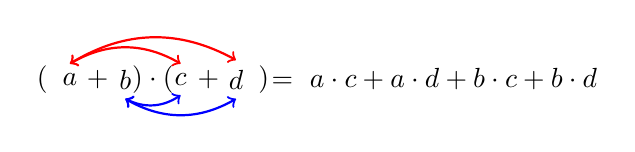
\begin{tikzpicture}[y=1em, x=1em,font=\sffamily]
    %% Draw the (a+b) part
    \node     at (0,0) {$($};
    \node (a) at (1,0) {$a$};
    \node     at (2,0) {$+$};
    \node (b) at (3,0) {$b$};
    \node     at (4,0) {$)\cdot($};

    %% Draw the *(c+d) part
    \node (c) at (5,0) {$c$};
    \node     at (6,0) {$+$};
    \node (d) at (7,0) {$d$};
    \node     at (8,0) {$)$};

    %% Draw the right hand side of the equation
    \node     at (14,0) {$~=~a\cdot c + a\cdot d + b\cdot c + b\cdot d$};

    %% Now make the pretty lines between the parts to FOIL
    \path[red,<->,thick] (a.north) edge[bend left] node {} (c.north);
    \path[red,<->,thick] (a.north) edge[bend left] node {} (d.north);

    \path[blue,<->,thick] (b.south) edge[bend right] node {} (c.south);
    \path[blue,<->,thick] (b.south) edge[bend right] node {} (d.south);

  \end{tikzpicture}

  \begin{subproblem}
  \item ${\displaystyle (x-3)^2}$
    \begin{eqnarray*}
      (x-3)^2 & = & (x-3)\cdot(x-3), \\
              & = & x\cdot x - 3\cdot x - 3\cdot x + (-3)\cdot(-3), \\
              & = & x^2 - 3x - 3x + 9, \\
              & = & x^2 - 6x + 9.
    \end{eqnarray*}
  \item ${\displaystyle (x+4)^2}$
    \vfill
  \item ${\displaystyle (y-5)^2}$
    \vfill
  \item ${\displaystyle (y+a)^2}$ where $a$ is a constant.
    \vfill
  \end{subproblem}
\item if $(x-a)^2=x^2+10x+25$ what is the value of $a$?
  \vfill
\end{problem}


\actTitle{Graphs of Equations}
\begin{problem}

\item Sketch the set of all points that are a distance of two from the
  point $Q(1,-3)$. What kind of figure do the points represent?

  \begin{tikzpicture}[y=1cm, x=1cm,font=\sffamily]
      % bounds
      \def\lowX{-5.5}
      \pgfmathtruncatemacro\startX{round(0.5+\lowX)}
      \pgfmathsetmacro\nextXValue{int(\startX+1)}
      \def\highX{5.5}
      \def\lowY{-5.5}
      \def\highY{5.5}
      \pgfmathsetmacro\nextYValue{int(\lowY+1)}
      % ticks
      \draw[step = 1, gray, very thin,dashed,opacity=0.85] (\lowX, \lowY) grid ( \highX,\highY);
   	% axis
  	\draw[thick,->] (\lowX,0) -- coordinate (x axis mid) (\highX,0) node[anchor = north west] {$x$};
      \draw[thick,->] (0,\lowY) -- coordinate (y axis mid) (0,\highY) node[anchor = south east] {$y$};
      \foreach \y in {-5,-4,...,-1,1,2,...,\highY} {
        \draw (1pt, \y) -- (-1pt, \y) node[yshift=-6,xshift=-1,anchor=east] {$\y$};
      }
      \foreach \x in {-5,-4,...,-1,1,2,...,\highX} {
        \draw (\x,1pt) -- (\x,-1pt) node[yshift=-5,xshift=-1,anchor=east] {$\x$};
      }
    \end{tikzpicture}


\item Suppose a point, $P(x,y)$ is a distance of $R$ units from the
  point $C(x_0,y_0)$.
  \sideNote{The values, $x_0$ and $y_0$, are constants. The notation
    is awkward, but this is a convention that we have to adapt to.}
  \begin{subproblem}
  \item Use the distance formula to express the distance relationship
    between $P$ and $C$.
    \vfill
  \item Square both sides of the previous equation.
    \vfill
  \end{subproblem}


\clearpage

\item Make a sketch of the circle with a radius of two centered at the
  point $P(-2,3)$. Determine a formula for the circle.

  \begin{tikzpicture}[y=1cm, x=1cm,font=\sffamily]
    % bounds
    \def\lowX{-5.5}
    \pgfmathtruncatemacro\startX{round(0.5+\lowX)}
    \pgfmathsetmacro\nextXValue{int(\startX+1)}
    \def\highX{5.5}
    \def\lowY{-5.5}
    \def\highY{5.5}
    \pgfmathsetmacro\nextYValue{int(\lowY+1)}
    % ticks
    \draw[step = 1, gray, very thin,dashed,opacity=0.85] (\lowX, \lowY) grid ( \highX,\highY);
 	% axis
	\draw[thick,->] (\lowX,0) -- coordinate (x axis mid) (\highX,0) node[anchor = north west] {$x$};
    \draw[thick,->] (0,\lowY) -- coordinate (y axis mid) (0,\highY) node[anchor = south east] {$y$};
    \foreach \y in {-5,-4,...,-1,1,2,...,\highY} {
      \draw (1pt, \y) -- (-1pt, \y) node[yshift=-6,xshift=-1,anchor=east] {$\y$};
    }
    \foreach \x in {-5,-4,...,-1,1,2,...,\highX} {
      \draw (\x,1pt) -- (\x,-1pt) node[yshift=-5,xshift=-1,anchor=east] {$\x$};
    }
  \end{tikzpicture}

  \clearpage

\item Sketch a graph of the relationship given by
  \begin{eqnarray*}
    x^2 + 2x + y^2 - 8y & = & 8.
  \end{eqnarray*}
  Determine the center and the radius of the circle.  Make a sketch of
  the circle. (Include the axes and label the axes.)  

  \vfill

  \clearpage

  In mathematics the idea of proportionality has a specific
  definition. The idea is that when two things are proportional then
  any changes in one yield a similar change in the other. For example,
  suppose we have two quantities. The first we call $x$, and the other
  we call $y$. If $y$ is proportional to $x$, then if we double $x$
  then $y$ will double. Likewise, if we triple $x$ then $y$ will
  triple.

  We express this mathematically by noting that if $y$ is proportional
  to $x$ then the ratio of $y$ to $x$ must be a constant,
  \begin{eqnarray*}
    \frac{y}{x} & = & \mathrm{constant}.
  \end{eqnarray*}
  If we multiply both sides by $x$ then
  \begin{eqnarray*}
    y & = & x \cdot \mathrm{constant}.
  \end{eqnarray*}

  As an example, it is estimated that the length of a person's femur
  is proportional to the person's total height. This implies that
  \begin{eqnarray*}
    \frac{\mathrm{height}}{\mathrm{femur ~ length}} & = & \mathrm{constant}.
  \end{eqnarray*}
  In a paper by Obialor \textit{et al}\footnote{Ambrose Obialor,
    Churchill Ihentuge and Frank Akpuaka, \textbf{Determination of
      Height Using Femur Length in Adult Population of Oguta Local
      Government Area of Imo State Nigeria}, The FASEB Journal, April
    2015, vol. 29 no. 1 Supplement LB19}, it is estimated that in a
  specific area in Nigeria the mean height of women is 161.90 cm and
  the mean femur length of women is 40.82 cm. If a woman's femur has a
  length of 42.00 cm, what is her expected height?

  First, we have to estimate the value of the constant. Assuming that
  the means are consistent then 
  \begin{eqnarray*}
    \frac{161.90}{40.82} & = & \mathrm{constant.}
  \end{eqnarray*}
  Now we look at the expression for the unidentified woman,
  \begin{eqnarray*}
    \frac{\mathrm{height}}{42.00} & = & \frac{161.90}{40.82}.
  \end{eqnarray*}
  Solving for the height we get
  \begin{eqnarray*}
    \mathrm{height} & = & 42.00\cdot\frac{161.90}{40.82} \mathrm{cm}.
  \end{eqnarray*}

  \clearpage

\item Windows are constructed, and their width is proportional to
  their height. One window is measured, and its width is 100cm, and its
  height is 200cm. 

  \begin{subproblem}

  \item Another window has a width of 75cm. What is its height?

    \vfill

  \item Make a sketch of the relationship of the height of a window
    given its width. First, express the relationship as a mathematical
    formula. Second, sketch the graph of the relationship. Briefly
    discuss the relationship. How does the height change as the width
    changes?  \sideNote{Annotate your plot and label your axes!}

    \vfill
    
  \end{subproblem}

  \clearpage

\item The surface area of a sparrow's wing is proportional to the
  square of the length of its wing. A sparrow is measured, and it has
  a wing length of 9cm and an area of 45cm\textsuperscript{2}. 

  \begin{subproblem}

  \item Another sparrow is measured, and the length of its wing is
    8cm. What is the area of its wing?

    \vfill

  \item Make a sketch of the relationship of the area of a sparrow's
    wing given the length. Briefly discuss the relationship. How does
    the area change as the length changes?  \sideNote{Annotate your
      plot and label your axes!}

    \vfill

  \end{subproblem}

  \vfill



\end{problem}

\postClass

\begin{problem}
\item Briefly state two ideas from today's class.
  \begin{itemize}
  \item
  \item
  \end{itemize}
\item A square is circumscribed within a circle of radius $R$ so it
  just touches the circle on each of the four corners of the square.

  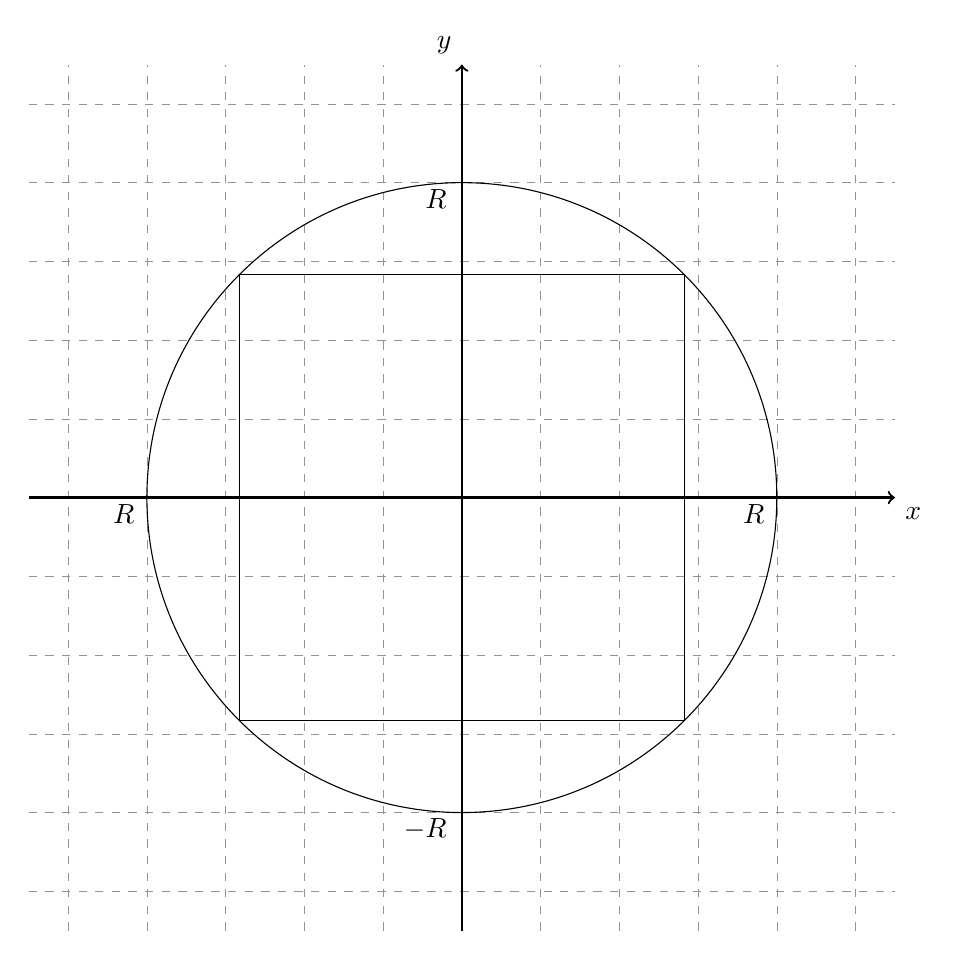
\begin{tikzpicture}[y=1cm, x=1cm,font=\sffamily]
    % bounds
    \def\lowX{-5.5}
    \pgfmathtruncatemacro\startX{round(0.5+\lowX)}
    \pgfmathsetmacro\nextXValue{int(\startX+1)}
    \def\highX{5.5}
    \def\lowY{-5.5}
    \def\highY{5.5}
    \pgfmathsetmacro\nextYValue{int(\lowY+1)}
    % ticks
    \draw[step = 1, gray, very thin,dashed,opacity=0.85] (\lowX, \lowY) grid ( \highX,\highY);
 	% axis
	\draw[thick,->] (\lowX,0) -- coordinate (x axis mid) (\highX,0) node[anchor = north west] {$x$};
    \draw[thick,->] (0,\lowY) -- coordinate (y axis mid) (0,\highY) node[anchor = south east] {$y$};

    \draw[black] (0:4) arc (0:360:4);
    \draw[black] (45:4) -- (135:4) -- (225:4) -- (315:4) -- (45:4);
    %\draw[black] (0:0) arc (0:30:0.2) node[midway,anchor=west] {$\theta$};

    \draw (1pt,  4) -- (-1pt,  4) node[yshift=-6,xshift=-1,anchor=east] {$R$};
    \draw (1pt, -4) -- (-1pt, -4) node[yshift=-6,xshift=-1,anchor=east] {$-R$};

    \draw ( 4,1pt) -- ( 4,-1pt) node[yshift=-5,xshift=-1,anchor=east] {$R$};
    \draw (-4,1pt) -- (-4,-1pt) node[yshift=-5,xshift=-1,anchor=east] {$R$};

  \end{tikzpicture}

  \begin{subproblem}
    \item Sketch the radius of the circle at one of the points where the square touches the circle.
    \item Find a convenient right triangle in the new diagram using
      the radius that you drew, and use the triangle to determine the
      length of one of the sides of the square. (You may have to
      double the length of the triangle to get the length of the
      side.)
    \item Determine the area of the square.
  \end{subproblem}

\item A triangle with three equal sides is circumscribed within a
  circle of radius $R$ so it just touches the circle on each of the
  three corners of the triangle.

  \begin{subproblem}
  \item Make a sketch of the situation. (Label your axes and label the
    length of the sides of the triangle.)
  \item Sketch the radius of the circle at one of the points where the
    triangle touches the circle.
  \item Find a convenient right triangle in the new diagram, and use
    the triangle to determine the length of one of the sides of the
    triangle. (You may have to double the length of the triangle to
    get the length of the side.)
  \end{subproblem}


\end{problem}



%%% Local Variables:
%%% mode: latex
%%% TeX-master: "functions"
%%% End:


%=========================================================================
% Start of 
%=========================================================================
\preClass{Introduction to Functions}

\begin{problem}
\item A biologist grows four different colonies of bacteria. The
  number of bacteria in the colonies is estimated to be 10,000,
  20,000, 30,000, and 40,000. The mass for each colony is measured and
  is estimated to be $2.61\times 10^{-6}$, $6.73\times 10^{-6}$,
  $8.24\times 10^{-6}$ and $1.12\times 10^{-7}$ grams respectively.

  Organize the information above into a table so that the mass can be
  more easily determined given the number of bacteria in the
  colony. Also, graph each point as a coordinate where the number of
  bacteria is on the horizontal axis, and the mass is on the vertical
  axis. 

  \vfill

\item Make rough estimate for a relationship that will provide a
  prediction for the mass of a colony given the number of bacteria
  within it.

  \vfill

\item Each time the number of bacteria increase by 10,000 what is the
  change in the mass?

  \vspace{5em}


\end{problem}


\actTitle{Functions}
\begin{problem}
\item A balloon has a tether to the ground, and it can be extended or
  retracted as the balloon is raised or lowered. One end of the tether
  is attached to the ground 20m away from a point directly below the
  balloon. If the balloon is $x$ meters high in the air what is the
  length of the tether?
  \begin{subproblem}
    \item Sketch a diagram of the situation. Label the known and
      unknown quantities.
      \sideNote{Assume that the balloon only moves up and down with no
        lateral motion.}
      \vfill
      \vfill
    \item Determine the important relationships between the known and
      unknown quantities.
      \vfill
    \item Determine the length of the tether given the height.
      \vfill
    \item Determine the domain and range of the function.
      \vfill
  \end{subproblem}

  \clearpage

\item A park has two distinct areas separated by a river, and each
  area has its own population of mice.  The population East of the
  river is estimated to have 10,000 individuals at the beginning of
  the year, and each week it grows by a constant 200 individuals. The
  population West of the river is estimated to have 8,000 individuals
  at the beginning of the year, and each week it grows by a constant
  250 individuals.

  \begin{subproblem}
  \item Make a rough sketch of the number of mice in the two
    populations on the same graph. The horizontal axis should be the
    time from the beginning of the year in weeks.
    \vfill

  \item Describe what is happening to the two populations. Is there a
    time when the two populations are equal? If so when is it?
    \vfill

  \item Determine a formula for the total number of mice in the park
    at any week after the beginning of the year.
    \vfill
  \end{subproblem}

  
\end{problem}

\postClass

\begin{problem}
\item Briefly state two ideas from today's class.
  \begin{itemize}
  \item 
  \item 
  \end{itemize}
\item 
  \begin{subproblem}
    \item
  \end{subproblem}
\end{problem}


%%% Local Variables:
%%% mode: latex
%%% TeX-master: "../labManual"
%%% End:



%=========================================================================
% Start of
%=========================================================================
\preClass{Linear Functions}

\begin{problem}
\item A tortoise and a hare move in a straight line, and the both
  start at $x=0$. The tortoise's position is given by
  \begin{eqnarray*}
    x_T & = & \frac{1}{2} t,
  \end{eqnarray*}
  where $t$ is in minutes and $x$ is in meters.  The hare's position
  is given by
  \begin{eqnarray*}
    x_H & = & 2 t,
  \end{eqnarray*}
  where $t$ is in minutes and $x$ is in meters.

  Determine the relationship between the hare's and the tortoise's
  position. That is, given the hare's position determine the
  tortoise's position. Make a sketch of the graph of the relationship using the axes below.

  \begin{tikzpicture}[y=1.1cm, x=1.1cm,font=\sffamily]
      % bounds
      \def\lowX{-5.5}
      \pgfmathtruncatemacro\startX{round(0.5+\lowX)}
      \pgfmathsetmacro\nextXValue{int(\startX+1)}
      \def\highX{5.5}
      \def\lowY{-5.5}
      \def\highY{5.5}
      \pgfmathsetmacro\nextYValue{int(\lowY+1)}
      % ticks
      \draw[step = 1, gray, very thin,dashed,opacity=0.85] (\lowX, \lowY) grid ( \highX,\highY);
    % axis
    \draw[thick,->] (\lowX,0) -- coordinate (x axis mid) (\highX,0) node[anchor = north west] {Hare};
      \draw[thick,->] (0,\lowY) -- coordinate (y axis mid) (0,\highY) node[anchor = north east] {Tortoise};
      \foreach \y in {-5,-4,...,-1,1,2,...,\highY} {
        \draw (1pt, \y) -- (-1pt, \y) node[yshift=-6,xshift=-1,anchor=east] {$\y$};
      }
      \foreach \x in {-5,-4,...,-1,1,2,...,\highX} {
        \draw (\x,1pt) -- (\x,-1pt) node[yshift=-5,xshift=-1,anchor=east] {$\x$};
      }
      \draw (0,5.5) node [anchor=south] {Hare vs. Tortoise};
    \end{tikzpicture}


    What is the tortoise's position when the hare's position is 15
    meters? (Mark the associated coordinate on the plot above.)


\end{problem}


\actTitle{Linear Equations}
\begin{problem}
\item In each case below determine the formulas for the lines that
  satisfy the given requirements. In each case make a rough sketch of
  the line.

  \begin{subproblem}
  \item Goes through the point $P(-2,5)$ and has a slope of -3.
    \vfill
  \item Goes through the points $P_1(-3,-4)$ and $P_2(4,1)$.
    \vfill
  \end{subproblem}

  \clearpage

\item Birds near a park are studied by a group of researchers. The
  birds tend to use cigarette butts in their nests, and it is believed
  to help reduce the number of parasitic insects. It is estimated that
  the number of cigarette butts used for nesting materials varies
  linearly with the distance from the nest to a nearby open air
  theater. A nest that is a distance of 30 meters appears to have 10
  cigarette butts, and a nest that is a distance of 40 meters appears
  to have 8 cigarette butts.
  \begin{subproblem}
  \item Determine the relationship that will predict the number of
    cigarette butts in a nest given its distance from the theater.
    Use it to predict the number of cigarette butts in a nest 50
    meters from the theater. Also, make a sketch of the relationship.
    \sideNote{Be sure to label your axes and annotate your plot.}

    \vfill
    \vfill
    \vfill

  \item What is the domain for the relationship?
    \vfill
  \item A nest is found that has 4 cigarette butts. What is the
    prediction for the distance the nest is from the theater.
    \vfill
  \item If the conjecture for the reason why birds use cigarette butts
    in their nests is true what would you expect is the general
    relationship between the fledgling success rate for birds and the
    location of their nests?
  \end{subproblem}


\end{problem}

\postClass

\begin{problem}
\item Briefly state two ideas from today's class.
  \begin{itemize}
  \item
  \item
  \end{itemize}
\item The growth rate for a population is the change in the number of individuals
  in a unit time. The per-capita growth rate is the growth rate divided by
  the total number of individuals.
  The per-capita growth rate for a species is approximated as a
  linear function. It is estimated that when the population is near
  zero the per-capita growth rate is highest due to a lack of
  competition and approaches 0.5 (the time units are hours). When the
  population approaches 1,000 the per-capita growth rate is estimated
  to be zero.
  \begin{subproblem}
    \item What are the units for the per capita growth rate?
    \item Determine the relationship that gives the per-capita growth
      rate as a function of the population, $p$.
    \item Make a sketch of the graph of the per-capita growth
      rate. (Make sure to annotate your graph and label your axes.)
    \item What happens to the per-capita growth rate as the population
      increases? Why might this happen?
    \item Determine the values where the per-capita growth rate is
      negative. Why would the per-capita growth rate be negative?
  \end{subproblem}
\end{problem}


%%% Local Variables:
%%% mode: latex
%%% TeX-master: "../labManual"
%%% End:


%=========================================================================
% Start of activity on linear models
%=========================================================================
\preClass{Linear Models}

\begin{problem}
\item A chemical reaction has a reactant that is broken down by
  itself, and the resulting reaction produces two different
  products. It is estimated that for each gram of the reactant that
  $\frac{1}{3}$g of the first product is produced and $\frac{1}{6}$g
  of the original reactant remains. Everything else that remains is
  the second product.
  \begin{subproblem}
  \item If you start with four grams of reactant how many grams of the
    products and the reactants will you get?
    \vfill
  \item Determine the number of grams of the products and reactants
    will result when you start with  $x$ grams of reactant.
    \vfill
  \end{subproblem}
\end{problem}


\actTitle{Modeling With Linear Functions}
\begin{problem}
\item 
  \begin{subproblem}
    \item
  \end{subproblem}
\end{problem}

\postClass

\begin{problem}
\item Briefly state two ideas from today's class.
  \begin{itemize}
  \item 
  \item 
  \end{itemize}
\item 
  \begin{subproblem}
    \item
  \end{subproblem}
\end{problem}



%=========================================================================
% Start of 
%=========================================================================
\preClass{Graphs of Functions}

\begin{problem}
\item Two populations of different species of bacteria interact. The
  number of bacteria (in millions) in the first population is given by
  \begin{eqnarray*}
    B(t) & = & 10 + t^2,
  \end{eqnarray*}
  where $t$ is the time in days since the beginning of the year.  The
  number of bacteria (in millions) in the second population is given by
  \begin{eqnarray*}
    C(t) & = & 10+(t-2)^2,
  \end{eqnarray*}
  where $t$ is the time in days since the beginning of the year.
  \begin{subproblem}
  \item Make a sketch of the two functions below.
    \vfill
  \item A researcher decides to alter the situation and adds 5 million
    bacteria to the first population given by $B(t)$. Determine a
    formula for the altered population. Make a sketch of the original
    and altered populations below.
    \vfill
  \end{subproblem}

\end{problem}


\actTitle{Graphs of Functions}
\begin{problem}
\item The height, in meters, of a certain tree changes by the
  relationship
  \begin{eqnarray*}
    h(t) & = & \sqrt{\frac{t}{3}},
  \end{eqnarray*}
  where $t$ is the time in years from when the seed was germinated. 
  \begin{subproblem}
  \item Make a sketch of the height of a tree as a function of time.
    \vfill
  \item Two seeds are planted, and the second seed germinates one year
    after the first is germinated. Determine the formulas for the
    height of the two trees with respect to the time that the first
    seed is germinated. Make a sketch of the two functions on the same
    graph.
    \vfill
  \item A new strain of the tree is developed that grows twice as fast
    as the original. Determine the formula that will give the height
    of the new strain. Make a sketch comparing the height of the
    original and the new strains.
    \vfill
  \end{subproblem}

  \clearpage

\item A function is defined to be
  \begin{eqnarray*}
    f(x) & = & |x|.
  \end{eqnarray*}
  \begin{subproblem}
  \item Make a sketch of the function on the axes below.
  \item Make a sketch of the following new functions on the graph as
    well with clear annotations:
    \begin{eqnarray*}
      g(x) & = & f(3x), \\
      h(x) & = & f(x)+2, \\
      p(x) & = & f(x+2), \\
      q(x) & = & 3f(x).
    \end{eqnarray*}

    \hspace*{-6em}
    \scalebox{0.95}{%% Creator: Matplotlib, PGF backend
%%
%% To include the figure in your LaTeX document, write
%%   \input{<filename>.pgf}
%%
%% Make sure the required packages are loaded in your preamble
%%   \usepackage{pgf}
%%
%% Figures using additional raster images can only be included by \input if
%% they are in the same directory as the main LaTeX file. For loading figures
%% from other directories you can use the `import` package
%%   \usepackage{import}
%% and then include the figures with
%%   \import{<path to file>}{<filename>.pgf}
%%
%% Matplotlib used the following preamble
%%   \usepackage{fontspec}
%%   \setmainfont{Bitstream Vera Serif}
%%   \setsansfont{Bitstream Vera Sans}
%%   \setmonofont{Bitstream Vera Sans Mono}
%%
\begingroup%
\makeatletter%
\begin{pgfpicture}%
\pgfpathrectangle{\pgfpointorigin}{\pgfqpoint{8.000000in}{6.000000in}}%
\pgfusepath{use as bounding box, clip}%
\begin{pgfscope}%
\pgfsetbuttcap%
\pgfsetmiterjoin%
\definecolor{currentfill}{rgb}{1.000000,1.000000,1.000000}%
\pgfsetfillcolor{currentfill}%
\pgfsetlinewidth{0.000000pt}%
\definecolor{currentstroke}{rgb}{1.000000,1.000000,1.000000}%
\pgfsetstrokecolor{currentstroke}%
\pgfsetdash{}{0pt}%
\pgfpathmoveto{\pgfqpoint{0.000000in}{0.000000in}}%
\pgfpathlineto{\pgfqpoint{8.000000in}{0.000000in}}%
\pgfpathlineto{\pgfqpoint{8.000000in}{6.000000in}}%
\pgfpathlineto{\pgfqpoint{0.000000in}{6.000000in}}%
\pgfpathclose%
\pgfusepath{fill}%
\end{pgfscope}%
\begin{pgfscope}%
\pgfsetbuttcap%
\pgfsetmiterjoin%
\definecolor{currentfill}{rgb}{1.000000,1.000000,1.000000}%
\pgfsetfillcolor{currentfill}%
\pgfsetlinewidth{0.000000pt}%
\definecolor{currentstroke}{rgb}{0.000000,0.000000,0.000000}%
\pgfsetstrokecolor{currentstroke}%
\pgfsetstrokeopacity{0.000000}%
\pgfsetdash{}{0pt}%
\pgfpathmoveto{\pgfqpoint{1.000000in}{0.600000in}}%
\pgfpathlineto{\pgfqpoint{7.200000in}{0.600000in}}%
\pgfpathlineto{\pgfqpoint{7.200000in}{5.400000in}}%
\pgfpathlineto{\pgfqpoint{1.000000in}{5.400000in}}%
\pgfpathclose%
\pgfusepath{fill}%
\end{pgfscope}%
\begin{pgfscope}%
\pgfsetrectcap%
\pgfsetmiterjoin%
\pgfsetlinewidth{0.000000pt}%
\definecolor{currentstroke}{rgb}{0.000000,0.000000,0.000000}%
\pgfsetstrokecolor{currentstroke}%
\pgfsetstrokeopacity{0.000000}%
\pgfsetdash{}{0pt}%
\pgfpathmoveto{\pgfqpoint{1.000000in}{5.400000in}}%
\pgfpathlineto{\pgfqpoint{7.200000in}{5.400000in}}%
\pgfusepath{}%
\end{pgfscope}%
\begin{pgfscope}%
\pgfsetrectcap%
\pgfsetmiterjoin%
\pgfsetlinewidth{0.000000pt}%
\definecolor{currentstroke}{rgb}{0.000000,0.000000,0.000000}%
\pgfsetstrokecolor{currentstroke}%
\pgfsetstrokeopacity{0.000000}%
\pgfsetdash{}{0pt}%
\pgfpathmoveto{\pgfqpoint{7.200000in}{0.600000in}}%
\pgfpathlineto{\pgfqpoint{7.200000in}{5.400000in}}%
\pgfusepath{}%
\end{pgfscope}%
\begin{pgfscope}%
\pgfsetrectcap%
\pgfsetmiterjoin%
\pgfsetlinewidth{1.003750pt}%
\definecolor{currentstroke}{rgb}{0.000000,0.000000,0.000000}%
\pgfsetstrokecolor{currentstroke}%
\pgfsetdash{}{0pt}%
\pgfpathmoveto{\pgfqpoint{1.000000in}{3.000000in}}%
\pgfpathlineto{\pgfqpoint{7.200000in}{3.000000in}}%
\pgfusepath{stroke}%
\end{pgfscope}%
\begin{pgfscope}%
\pgfsetrectcap%
\pgfsetmiterjoin%
\pgfsetlinewidth{1.003750pt}%
\definecolor{currentstroke}{rgb}{0.000000,0.000000,0.000000}%
\pgfsetstrokecolor{currentstroke}%
\pgfsetdash{}{0pt}%
\pgfpathmoveto{\pgfqpoint{4.100000in}{0.600000in}}%
\pgfpathlineto{\pgfqpoint{4.100000in}{5.400000in}}%
\pgfusepath{stroke}%
\end{pgfscope}%
\begin{pgfscope}%
\pgfsetbuttcap%
\pgfsetroundjoin%
\pgfsetlinewidth{0.501875pt}%
\definecolor{currentstroke}{rgb}{0.000000,0.000000,0.000000}%
\pgfsetstrokecolor{currentstroke}%
\pgfsetdash{{1.000000pt}{3.000000pt}}{0.000000pt}%
\pgfpathmoveto{\pgfqpoint{1.060784in}{0.600000in}}%
\pgfpathlineto{\pgfqpoint{1.060784in}{5.400000in}}%
\pgfusepath{stroke}%
\end{pgfscope}%
\begin{pgfscope}%
\pgfsetbuttcap%
\pgfsetroundjoin%
\definecolor{currentfill}{rgb}{0.000000,0.000000,0.000000}%
\pgfsetfillcolor{currentfill}%
\pgfsetlinewidth{0.501875pt}%
\definecolor{currentstroke}{rgb}{0.000000,0.000000,0.000000}%
\pgfsetstrokecolor{currentstroke}%
\pgfsetdash{}{0pt}%
\pgfsys@defobject{currentmarker}{\pgfqpoint{0.000000in}{0.000000in}}{\pgfqpoint{0.000000in}{0.055556in}}{%
\pgfpathmoveto{\pgfqpoint{0.000000in}{0.000000in}}%
\pgfpathlineto{\pgfqpoint{0.000000in}{0.055556in}}%
\pgfusepath{stroke,fill}%
}%
\begin{pgfscope}%
\pgfsys@transformshift{1.060784in}{3.000000in}%
\pgfsys@useobject{currentmarker}{}%
\end{pgfscope}%
\end{pgfscope}%
\begin{pgfscope}%
\pgftext[x=1.060784in,y=2.944444in,,top]{\sffamily\fontsize{12.000000}{14.400000}\selectfont -5}%
\end{pgfscope}%
\begin{pgfscope}%
\pgfsetbuttcap%
\pgfsetroundjoin%
\pgfsetlinewidth{0.501875pt}%
\definecolor{currentstroke}{rgb}{0.000000,0.000000,0.000000}%
\pgfsetstrokecolor{currentstroke}%
\pgfsetdash{{1.000000pt}{3.000000pt}}{0.000000pt}%
\pgfpathmoveto{\pgfqpoint{1.668627in}{0.600000in}}%
\pgfpathlineto{\pgfqpoint{1.668627in}{5.400000in}}%
\pgfusepath{stroke}%
\end{pgfscope}%
\begin{pgfscope}%
\pgfsetbuttcap%
\pgfsetroundjoin%
\definecolor{currentfill}{rgb}{0.000000,0.000000,0.000000}%
\pgfsetfillcolor{currentfill}%
\pgfsetlinewidth{0.501875pt}%
\definecolor{currentstroke}{rgb}{0.000000,0.000000,0.000000}%
\pgfsetstrokecolor{currentstroke}%
\pgfsetdash{}{0pt}%
\pgfsys@defobject{currentmarker}{\pgfqpoint{0.000000in}{0.000000in}}{\pgfqpoint{0.000000in}{0.055556in}}{%
\pgfpathmoveto{\pgfqpoint{0.000000in}{0.000000in}}%
\pgfpathlineto{\pgfqpoint{0.000000in}{0.055556in}}%
\pgfusepath{stroke,fill}%
}%
\begin{pgfscope}%
\pgfsys@transformshift{1.668627in}{3.000000in}%
\pgfsys@useobject{currentmarker}{}%
\end{pgfscope}%
\end{pgfscope}%
\begin{pgfscope}%
\pgftext[x=1.668627in,y=2.944444in,,top]{\sffamily\fontsize{12.000000}{14.400000}\selectfont -4}%
\end{pgfscope}%
\begin{pgfscope}%
\pgfsetbuttcap%
\pgfsetroundjoin%
\pgfsetlinewidth{0.501875pt}%
\definecolor{currentstroke}{rgb}{0.000000,0.000000,0.000000}%
\pgfsetstrokecolor{currentstroke}%
\pgfsetdash{{1.000000pt}{3.000000pt}}{0.000000pt}%
\pgfpathmoveto{\pgfqpoint{2.276471in}{0.600000in}}%
\pgfpathlineto{\pgfqpoint{2.276471in}{5.400000in}}%
\pgfusepath{stroke}%
\end{pgfscope}%
\begin{pgfscope}%
\pgfsetbuttcap%
\pgfsetroundjoin%
\definecolor{currentfill}{rgb}{0.000000,0.000000,0.000000}%
\pgfsetfillcolor{currentfill}%
\pgfsetlinewidth{0.501875pt}%
\definecolor{currentstroke}{rgb}{0.000000,0.000000,0.000000}%
\pgfsetstrokecolor{currentstroke}%
\pgfsetdash{}{0pt}%
\pgfsys@defobject{currentmarker}{\pgfqpoint{0.000000in}{0.000000in}}{\pgfqpoint{0.000000in}{0.055556in}}{%
\pgfpathmoveto{\pgfqpoint{0.000000in}{0.000000in}}%
\pgfpathlineto{\pgfqpoint{0.000000in}{0.055556in}}%
\pgfusepath{stroke,fill}%
}%
\begin{pgfscope}%
\pgfsys@transformshift{2.276471in}{3.000000in}%
\pgfsys@useobject{currentmarker}{}%
\end{pgfscope}%
\end{pgfscope}%
\begin{pgfscope}%
\pgftext[x=2.276471in,y=2.944444in,,top]{\sffamily\fontsize{12.000000}{14.400000}\selectfont -3}%
\end{pgfscope}%
\begin{pgfscope}%
\pgfsetbuttcap%
\pgfsetroundjoin%
\pgfsetlinewidth{0.501875pt}%
\definecolor{currentstroke}{rgb}{0.000000,0.000000,0.000000}%
\pgfsetstrokecolor{currentstroke}%
\pgfsetdash{{1.000000pt}{3.000000pt}}{0.000000pt}%
\pgfpathmoveto{\pgfqpoint{2.884314in}{0.600000in}}%
\pgfpathlineto{\pgfqpoint{2.884314in}{5.400000in}}%
\pgfusepath{stroke}%
\end{pgfscope}%
\begin{pgfscope}%
\pgfsetbuttcap%
\pgfsetroundjoin%
\definecolor{currentfill}{rgb}{0.000000,0.000000,0.000000}%
\pgfsetfillcolor{currentfill}%
\pgfsetlinewidth{0.501875pt}%
\definecolor{currentstroke}{rgb}{0.000000,0.000000,0.000000}%
\pgfsetstrokecolor{currentstroke}%
\pgfsetdash{}{0pt}%
\pgfsys@defobject{currentmarker}{\pgfqpoint{0.000000in}{0.000000in}}{\pgfqpoint{0.000000in}{0.055556in}}{%
\pgfpathmoveto{\pgfqpoint{0.000000in}{0.000000in}}%
\pgfpathlineto{\pgfqpoint{0.000000in}{0.055556in}}%
\pgfusepath{stroke,fill}%
}%
\begin{pgfscope}%
\pgfsys@transformshift{2.884314in}{3.000000in}%
\pgfsys@useobject{currentmarker}{}%
\end{pgfscope}%
\end{pgfscope}%
\begin{pgfscope}%
\pgftext[x=2.884314in,y=2.944444in,,top]{\sffamily\fontsize{12.000000}{14.400000}\selectfont -2}%
\end{pgfscope}%
\begin{pgfscope}%
\pgfsetbuttcap%
\pgfsetroundjoin%
\pgfsetlinewidth{0.501875pt}%
\definecolor{currentstroke}{rgb}{0.000000,0.000000,0.000000}%
\pgfsetstrokecolor{currentstroke}%
\pgfsetdash{{1.000000pt}{3.000000pt}}{0.000000pt}%
\pgfpathmoveto{\pgfqpoint{3.492157in}{0.600000in}}%
\pgfpathlineto{\pgfqpoint{3.492157in}{5.400000in}}%
\pgfusepath{stroke}%
\end{pgfscope}%
\begin{pgfscope}%
\pgfsetbuttcap%
\pgfsetroundjoin%
\definecolor{currentfill}{rgb}{0.000000,0.000000,0.000000}%
\pgfsetfillcolor{currentfill}%
\pgfsetlinewidth{0.501875pt}%
\definecolor{currentstroke}{rgb}{0.000000,0.000000,0.000000}%
\pgfsetstrokecolor{currentstroke}%
\pgfsetdash{}{0pt}%
\pgfsys@defobject{currentmarker}{\pgfqpoint{0.000000in}{0.000000in}}{\pgfqpoint{0.000000in}{0.055556in}}{%
\pgfpathmoveto{\pgfqpoint{0.000000in}{0.000000in}}%
\pgfpathlineto{\pgfqpoint{0.000000in}{0.055556in}}%
\pgfusepath{stroke,fill}%
}%
\begin{pgfscope}%
\pgfsys@transformshift{3.492157in}{3.000000in}%
\pgfsys@useobject{currentmarker}{}%
\end{pgfscope}%
\end{pgfscope}%
\begin{pgfscope}%
\pgftext[x=3.492157in,y=2.944444in,,top]{\sffamily\fontsize{12.000000}{14.400000}\selectfont -1}%
\end{pgfscope}%
\begin{pgfscope}%
\pgfsetbuttcap%
\pgfsetroundjoin%
\pgfsetlinewidth{0.501875pt}%
\definecolor{currentstroke}{rgb}{0.000000,0.000000,0.000000}%
\pgfsetstrokecolor{currentstroke}%
\pgfsetdash{{1.000000pt}{3.000000pt}}{0.000000pt}%
\pgfpathmoveto{\pgfqpoint{4.100000in}{0.600000in}}%
\pgfpathlineto{\pgfqpoint{4.100000in}{5.400000in}}%
\pgfusepath{stroke}%
\end{pgfscope}%
\begin{pgfscope}%
\pgfsetbuttcap%
\pgfsetroundjoin%
\definecolor{currentfill}{rgb}{0.000000,0.000000,0.000000}%
\pgfsetfillcolor{currentfill}%
\pgfsetlinewidth{0.501875pt}%
\definecolor{currentstroke}{rgb}{0.000000,0.000000,0.000000}%
\pgfsetstrokecolor{currentstroke}%
\pgfsetdash{}{0pt}%
\pgfsys@defobject{currentmarker}{\pgfqpoint{0.000000in}{0.000000in}}{\pgfqpoint{0.000000in}{0.055556in}}{%
\pgfpathmoveto{\pgfqpoint{0.000000in}{0.000000in}}%
\pgfpathlineto{\pgfqpoint{0.000000in}{0.055556in}}%
\pgfusepath{stroke,fill}%
}%
\begin{pgfscope}%
\pgfsys@transformshift{4.100000in}{3.000000in}%
\pgfsys@useobject{currentmarker}{}%
\end{pgfscope}%
\end{pgfscope}%
\begin{pgfscope}%
\pgftext[x=4.100000in,y=2.944444in,,top]{\sffamily\fontsize{12.000000}{14.400000}\selectfont 0}%
\end{pgfscope}%
\begin{pgfscope}%
\pgfsetbuttcap%
\pgfsetroundjoin%
\pgfsetlinewidth{0.501875pt}%
\definecolor{currentstroke}{rgb}{0.000000,0.000000,0.000000}%
\pgfsetstrokecolor{currentstroke}%
\pgfsetdash{{1.000000pt}{3.000000pt}}{0.000000pt}%
\pgfpathmoveto{\pgfqpoint{4.707843in}{0.600000in}}%
\pgfpathlineto{\pgfqpoint{4.707843in}{5.400000in}}%
\pgfusepath{stroke}%
\end{pgfscope}%
\begin{pgfscope}%
\pgfsetbuttcap%
\pgfsetroundjoin%
\definecolor{currentfill}{rgb}{0.000000,0.000000,0.000000}%
\pgfsetfillcolor{currentfill}%
\pgfsetlinewidth{0.501875pt}%
\definecolor{currentstroke}{rgb}{0.000000,0.000000,0.000000}%
\pgfsetstrokecolor{currentstroke}%
\pgfsetdash{}{0pt}%
\pgfsys@defobject{currentmarker}{\pgfqpoint{0.000000in}{0.000000in}}{\pgfqpoint{0.000000in}{0.055556in}}{%
\pgfpathmoveto{\pgfqpoint{0.000000in}{0.000000in}}%
\pgfpathlineto{\pgfqpoint{0.000000in}{0.055556in}}%
\pgfusepath{stroke,fill}%
}%
\begin{pgfscope}%
\pgfsys@transformshift{4.707843in}{3.000000in}%
\pgfsys@useobject{currentmarker}{}%
\end{pgfscope}%
\end{pgfscope}%
\begin{pgfscope}%
\pgftext[x=4.707843in,y=2.944444in,,top]{\sffamily\fontsize{12.000000}{14.400000}\selectfont 1}%
\end{pgfscope}%
\begin{pgfscope}%
\pgfsetbuttcap%
\pgfsetroundjoin%
\pgfsetlinewidth{0.501875pt}%
\definecolor{currentstroke}{rgb}{0.000000,0.000000,0.000000}%
\pgfsetstrokecolor{currentstroke}%
\pgfsetdash{{1.000000pt}{3.000000pt}}{0.000000pt}%
\pgfpathmoveto{\pgfqpoint{5.315686in}{0.600000in}}%
\pgfpathlineto{\pgfqpoint{5.315686in}{5.400000in}}%
\pgfusepath{stroke}%
\end{pgfscope}%
\begin{pgfscope}%
\pgfsetbuttcap%
\pgfsetroundjoin%
\definecolor{currentfill}{rgb}{0.000000,0.000000,0.000000}%
\pgfsetfillcolor{currentfill}%
\pgfsetlinewidth{0.501875pt}%
\definecolor{currentstroke}{rgb}{0.000000,0.000000,0.000000}%
\pgfsetstrokecolor{currentstroke}%
\pgfsetdash{}{0pt}%
\pgfsys@defobject{currentmarker}{\pgfqpoint{0.000000in}{0.000000in}}{\pgfqpoint{0.000000in}{0.055556in}}{%
\pgfpathmoveto{\pgfqpoint{0.000000in}{0.000000in}}%
\pgfpathlineto{\pgfqpoint{0.000000in}{0.055556in}}%
\pgfusepath{stroke,fill}%
}%
\begin{pgfscope}%
\pgfsys@transformshift{5.315686in}{3.000000in}%
\pgfsys@useobject{currentmarker}{}%
\end{pgfscope}%
\end{pgfscope}%
\begin{pgfscope}%
\pgftext[x=5.315686in,y=2.944444in,,top]{\sffamily\fontsize{12.000000}{14.400000}\selectfont 2}%
\end{pgfscope}%
\begin{pgfscope}%
\pgfsetbuttcap%
\pgfsetroundjoin%
\pgfsetlinewidth{0.501875pt}%
\definecolor{currentstroke}{rgb}{0.000000,0.000000,0.000000}%
\pgfsetstrokecolor{currentstroke}%
\pgfsetdash{{1.000000pt}{3.000000pt}}{0.000000pt}%
\pgfpathmoveto{\pgfqpoint{5.923529in}{0.600000in}}%
\pgfpathlineto{\pgfqpoint{5.923529in}{5.400000in}}%
\pgfusepath{stroke}%
\end{pgfscope}%
\begin{pgfscope}%
\pgfsetbuttcap%
\pgfsetroundjoin%
\definecolor{currentfill}{rgb}{0.000000,0.000000,0.000000}%
\pgfsetfillcolor{currentfill}%
\pgfsetlinewidth{0.501875pt}%
\definecolor{currentstroke}{rgb}{0.000000,0.000000,0.000000}%
\pgfsetstrokecolor{currentstroke}%
\pgfsetdash{}{0pt}%
\pgfsys@defobject{currentmarker}{\pgfqpoint{0.000000in}{0.000000in}}{\pgfqpoint{0.000000in}{0.055556in}}{%
\pgfpathmoveto{\pgfqpoint{0.000000in}{0.000000in}}%
\pgfpathlineto{\pgfqpoint{0.000000in}{0.055556in}}%
\pgfusepath{stroke,fill}%
}%
\begin{pgfscope}%
\pgfsys@transformshift{5.923529in}{3.000000in}%
\pgfsys@useobject{currentmarker}{}%
\end{pgfscope}%
\end{pgfscope}%
\begin{pgfscope}%
\pgftext[x=5.923529in,y=2.944444in,,top]{\sffamily\fontsize{12.000000}{14.400000}\selectfont 3}%
\end{pgfscope}%
\begin{pgfscope}%
\pgfsetbuttcap%
\pgfsetroundjoin%
\pgfsetlinewidth{0.501875pt}%
\definecolor{currentstroke}{rgb}{0.000000,0.000000,0.000000}%
\pgfsetstrokecolor{currentstroke}%
\pgfsetdash{{1.000000pt}{3.000000pt}}{0.000000pt}%
\pgfpathmoveto{\pgfqpoint{6.531373in}{0.600000in}}%
\pgfpathlineto{\pgfqpoint{6.531373in}{5.400000in}}%
\pgfusepath{stroke}%
\end{pgfscope}%
\begin{pgfscope}%
\pgfsetbuttcap%
\pgfsetroundjoin%
\definecolor{currentfill}{rgb}{0.000000,0.000000,0.000000}%
\pgfsetfillcolor{currentfill}%
\pgfsetlinewidth{0.501875pt}%
\definecolor{currentstroke}{rgb}{0.000000,0.000000,0.000000}%
\pgfsetstrokecolor{currentstroke}%
\pgfsetdash{}{0pt}%
\pgfsys@defobject{currentmarker}{\pgfqpoint{0.000000in}{0.000000in}}{\pgfqpoint{0.000000in}{0.055556in}}{%
\pgfpathmoveto{\pgfqpoint{0.000000in}{0.000000in}}%
\pgfpathlineto{\pgfqpoint{0.000000in}{0.055556in}}%
\pgfusepath{stroke,fill}%
}%
\begin{pgfscope}%
\pgfsys@transformshift{6.531373in}{3.000000in}%
\pgfsys@useobject{currentmarker}{}%
\end{pgfscope}%
\end{pgfscope}%
\begin{pgfscope}%
\pgftext[x=6.531373in,y=2.944444in,,top]{\sffamily\fontsize{12.000000}{14.400000}\selectfont 4}%
\end{pgfscope}%
\begin{pgfscope}%
\pgfsetbuttcap%
\pgfsetroundjoin%
\pgfsetlinewidth{0.501875pt}%
\definecolor{currentstroke}{rgb}{0.000000,0.000000,0.000000}%
\pgfsetstrokecolor{currentstroke}%
\pgfsetdash{{1.000000pt}{3.000000pt}}{0.000000pt}%
\pgfpathmoveto{\pgfqpoint{7.139216in}{0.600000in}}%
\pgfpathlineto{\pgfqpoint{7.139216in}{5.400000in}}%
\pgfusepath{stroke}%
\end{pgfscope}%
\begin{pgfscope}%
\pgfsetbuttcap%
\pgfsetroundjoin%
\definecolor{currentfill}{rgb}{0.000000,0.000000,0.000000}%
\pgfsetfillcolor{currentfill}%
\pgfsetlinewidth{0.501875pt}%
\definecolor{currentstroke}{rgb}{0.000000,0.000000,0.000000}%
\pgfsetstrokecolor{currentstroke}%
\pgfsetdash{}{0pt}%
\pgfsys@defobject{currentmarker}{\pgfqpoint{0.000000in}{0.000000in}}{\pgfqpoint{0.000000in}{0.055556in}}{%
\pgfpathmoveto{\pgfqpoint{0.000000in}{0.000000in}}%
\pgfpathlineto{\pgfqpoint{0.000000in}{0.055556in}}%
\pgfusepath{stroke,fill}%
}%
\begin{pgfscope}%
\pgfsys@transformshift{7.139216in}{3.000000in}%
\pgfsys@useobject{currentmarker}{}%
\end{pgfscope}%
\end{pgfscope}%
\begin{pgfscope}%
\pgftext[x=7.139216in,y=2.944444in,,top]{\sffamily\fontsize{12.000000}{14.400000}\selectfont 5}%
\end{pgfscope}%
\begin{pgfscope}%
\pgftext[x=4.100000in,y=2.713705in,,top]{\sffamily\fontsize{12.000000}{14.400000}\selectfont x}%
\end{pgfscope}%
\begin{pgfscope}%
\pgfsetbuttcap%
\pgfsetroundjoin%
\pgfsetlinewidth{0.501875pt}%
\definecolor{currentstroke}{rgb}{0.000000,0.000000,0.000000}%
\pgfsetstrokecolor{currentstroke}%
\pgfsetdash{{1.000000pt}{3.000000pt}}{0.000000pt}%
\pgfpathmoveto{\pgfqpoint{1.000000in}{0.647059in}}%
\pgfpathlineto{\pgfqpoint{7.200000in}{0.647059in}}%
\pgfusepath{stroke}%
\end{pgfscope}%
\begin{pgfscope}%
\pgfsetbuttcap%
\pgfsetroundjoin%
\definecolor{currentfill}{rgb}{0.000000,0.000000,0.000000}%
\pgfsetfillcolor{currentfill}%
\pgfsetlinewidth{0.501875pt}%
\definecolor{currentstroke}{rgb}{0.000000,0.000000,0.000000}%
\pgfsetstrokecolor{currentstroke}%
\pgfsetdash{}{0pt}%
\pgfsys@defobject{currentmarker}{\pgfqpoint{0.000000in}{0.000000in}}{\pgfqpoint{0.055556in}{0.000000in}}{%
\pgfpathmoveto{\pgfqpoint{0.000000in}{0.000000in}}%
\pgfpathlineto{\pgfqpoint{0.055556in}{0.000000in}}%
\pgfusepath{stroke,fill}%
}%
\begin{pgfscope}%
\pgfsys@transformshift{4.100000in}{0.647059in}%
\pgfsys@useobject{currentmarker}{}%
\end{pgfscope}%
\end{pgfscope}%
\begin{pgfscope}%
\pgftext[x=4.044444in,y=0.647059in,right,]{\sffamily\fontsize{12.000000}{14.400000}\selectfont -5}%
\end{pgfscope}%
\begin{pgfscope}%
\pgfsetbuttcap%
\pgfsetroundjoin%
\pgfsetlinewidth{0.501875pt}%
\definecolor{currentstroke}{rgb}{0.000000,0.000000,0.000000}%
\pgfsetstrokecolor{currentstroke}%
\pgfsetdash{{1.000000pt}{3.000000pt}}{0.000000pt}%
\pgfpathmoveto{\pgfqpoint{1.000000in}{1.117647in}}%
\pgfpathlineto{\pgfqpoint{7.200000in}{1.117647in}}%
\pgfusepath{stroke}%
\end{pgfscope}%
\begin{pgfscope}%
\pgfsetbuttcap%
\pgfsetroundjoin%
\definecolor{currentfill}{rgb}{0.000000,0.000000,0.000000}%
\pgfsetfillcolor{currentfill}%
\pgfsetlinewidth{0.501875pt}%
\definecolor{currentstroke}{rgb}{0.000000,0.000000,0.000000}%
\pgfsetstrokecolor{currentstroke}%
\pgfsetdash{}{0pt}%
\pgfsys@defobject{currentmarker}{\pgfqpoint{0.000000in}{0.000000in}}{\pgfqpoint{0.055556in}{0.000000in}}{%
\pgfpathmoveto{\pgfqpoint{0.000000in}{0.000000in}}%
\pgfpathlineto{\pgfqpoint{0.055556in}{0.000000in}}%
\pgfusepath{stroke,fill}%
}%
\begin{pgfscope}%
\pgfsys@transformshift{4.100000in}{1.117647in}%
\pgfsys@useobject{currentmarker}{}%
\end{pgfscope}%
\end{pgfscope}%
\begin{pgfscope}%
\pgftext[x=4.044444in,y=1.117647in,right,]{\sffamily\fontsize{12.000000}{14.400000}\selectfont -4}%
\end{pgfscope}%
\begin{pgfscope}%
\pgfsetbuttcap%
\pgfsetroundjoin%
\pgfsetlinewidth{0.501875pt}%
\definecolor{currentstroke}{rgb}{0.000000,0.000000,0.000000}%
\pgfsetstrokecolor{currentstroke}%
\pgfsetdash{{1.000000pt}{3.000000pt}}{0.000000pt}%
\pgfpathmoveto{\pgfqpoint{1.000000in}{1.588235in}}%
\pgfpathlineto{\pgfqpoint{7.200000in}{1.588235in}}%
\pgfusepath{stroke}%
\end{pgfscope}%
\begin{pgfscope}%
\pgfsetbuttcap%
\pgfsetroundjoin%
\definecolor{currentfill}{rgb}{0.000000,0.000000,0.000000}%
\pgfsetfillcolor{currentfill}%
\pgfsetlinewidth{0.501875pt}%
\definecolor{currentstroke}{rgb}{0.000000,0.000000,0.000000}%
\pgfsetstrokecolor{currentstroke}%
\pgfsetdash{}{0pt}%
\pgfsys@defobject{currentmarker}{\pgfqpoint{0.000000in}{0.000000in}}{\pgfqpoint{0.055556in}{0.000000in}}{%
\pgfpathmoveto{\pgfqpoint{0.000000in}{0.000000in}}%
\pgfpathlineto{\pgfqpoint{0.055556in}{0.000000in}}%
\pgfusepath{stroke,fill}%
}%
\begin{pgfscope}%
\pgfsys@transformshift{4.100000in}{1.588235in}%
\pgfsys@useobject{currentmarker}{}%
\end{pgfscope}%
\end{pgfscope}%
\begin{pgfscope}%
\pgftext[x=4.044444in,y=1.588235in,right,]{\sffamily\fontsize{12.000000}{14.400000}\selectfont -3}%
\end{pgfscope}%
\begin{pgfscope}%
\pgfsetbuttcap%
\pgfsetroundjoin%
\pgfsetlinewidth{0.501875pt}%
\definecolor{currentstroke}{rgb}{0.000000,0.000000,0.000000}%
\pgfsetstrokecolor{currentstroke}%
\pgfsetdash{{1.000000pt}{3.000000pt}}{0.000000pt}%
\pgfpathmoveto{\pgfqpoint{1.000000in}{2.058824in}}%
\pgfpathlineto{\pgfqpoint{7.200000in}{2.058824in}}%
\pgfusepath{stroke}%
\end{pgfscope}%
\begin{pgfscope}%
\pgfsetbuttcap%
\pgfsetroundjoin%
\definecolor{currentfill}{rgb}{0.000000,0.000000,0.000000}%
\pgfsetfillcolor{currentfill}%
\pgfsetlinewidth{0.501875pt}%
\definecolor{currentstroke}{rgb}{0.000000,0.000000,0.000000}%
\pgfsetstrokecolor{currentstroke}%
\pgfsetdash{}{0pt}%
\pgfsys@defobject{currentmarker}{\pgfqpoint{0.000000in}{0.000000in}}{\pgfqpoint{0.055556in}{0.000000in}}{%
\pgfpathmoveto{\pgfqpoint{0.000000in}{0.000000in}}%
\pgfpathlineto{\pgfqpoint{0.055556in}{0.000000in}}%
\pgfusepath{stroke,fill}%
}%
\begin{pgfscope}%
\pgfsys@transformshift{4.100000in}{2.058824in}%
\pgfsys@useobject{currentmarker}{}%
\end{pgfscope}%
\end{pgfscope}%
\begin{pgfscope}%
\pgftext[x=4.044444in,y=2.058824in,right,]{\sffamily\fontsize{12.000000}{14.400000}\selectfont -2}%
\end{pgfscope}%
\begin{pgfscope}%
\pgfsetbuttcap%
\pgfsetroundjoin%
\pgfsetlinewidth{0.501875pt}%
\definecolor{currentstroke}{rgb}{0.000000,0.000000,0.000000}%
\pgfsetstrokecolor{currentstroke}%
\pgfsetdash{{1.000000pt}{3.000000pt}}{0.000000pt}%
\pgfpathmoveto{\pgfqpoint{1.000000in}{2.529412in}}%
\pgfpathlineto{\pgfqpoint{7.200000in}{2.529412in}}%
\pgfusepath{stroke}%
\end{pgfscope}%
\begin{pgfscope}%
\pgfsetbuttcap%
\pgfsetroundjoin%
\definecolor{currentfill}{rgb}{0.000000,0.000000,0.000000}%
\pgfsetfillcolor{currentfill}%
\pgfsetlinewidth{0.501875pt}%
\definecolor{currentstroke}{rgb}{0.000000,0.000000,0.000000}%
\pgfsetstrokecolor{currentstroke}%
\pgfsetdash{}{0pt}%
\pgfsys@defobject{currentmarker}{\pgfqpoint{0.000000in}{0.000000in}}{\pgfqpoint{0.055556in}{0.000000in}}{%
\pgfpathmoveto{\pgfqpoint{0.000000in}{0.000000in}}%
\pgfpathlineto{\pgfqpoint{0.055556in}{0.000000in}}%
\pgfusepath{stroke,fill}%
}%
\begin{pgfscope}%
\pgfsys@transformshift{4.100000in}{2.529412in}%
\pgfsys@useobject{currentmarker}{}%
\end{pgfscope}%
\end{pgfscope}%
\begin{pgfscope}%
\pgftext[x=4.044444in,y=2.529412in,right,]{\sffamily\fontsize{12.000000}{14.400000}\selectfont -1}%
\end{pgfscope}%
\begin{pgfscope}%
\pgfsetbuttcap%
\pgfsetroundjoin%
\pgfsetlinewidth{0.501875pt}%
\definecolor{currentstroke}{rgb}{0.000000,0.000000,0.000000}%
\pgfsetstrokecolor{currentstroke}%
\pgfsetdash{{1.000000pt}{3.000000pt}}{0.000000pt}%
\pgfpathmoveto{\pgfqpoint{1.000000in}{3.000000in}}%
\pgfpathlineto{\pgfqpoint{7.200000in}{3.000000in}}%
\pgfusepath{stroke}%
\end{pgfscope}%
\begin{pgfscope}%
\pgfsetbuttcap%
\pgfsetroundjoin%
\definecolor{currentfill}{rgb}{0.000000,0.000000,0.000000}%
\pgfsetfillcolor{currentfill}%
\pgfsetlinewidth{0.501875pt}%
\definecolor{currentstroke}{rgb}{0.000000,0.000000,0.000000}%
\pgfsetstrokecolor{currentstroke}%
\pgfsetdash{}{0pt}%
\pgfsys@defobject{currentmarker}{\pgfqpoint{0.000000in}{0.000000in}}{\pgfqpoint{0.055556in}{0.000000in}}{%
\pgfpathmoveto{\pgfqpoint{0.000000in}{0.000000in}}%
\pgfpathlineto{\pgfqpoint{0.055556in}{0.000000in}}%
\pgfusepath{stroke,fill}%
}%
\begin{pgfscope}%
\pgfsys@transformshift{4.100000in}{3.000000in}%
\pgfsys@useobject{currentmarker}{}%
\end{pgfscope}%
\end{pgfscope}%
\begin{pgfscope}%
\pgftext[x=4.044444in,y=3.000000in,right,]{\sffamily\fontsize{12.000000}{14.400000}\selectfont 0}%
\end{pgfscope}%
\begin{pgfscope}%
\pgfsetbuttcap%
\pgfsetroundjoin%
\pgfsetlinewidth{0.501875pt}%
\definecolor{currentstroke}{rgb}{0.000000,0.000000,0.000000}%
\pgfsetstrokecolor{currentstroke}%
\pgfsetdash{{1.000000pt}{3.000000pt}}{0.000000pt}%
\pgfpathmoveto{\pgfqpoint{1.000000in}{3.470588in}}%
\pgfpathlineto{\pgfqpoint{7.200000in}{3.470588in}}%
\pgfusepath{stroke}%
\end{pgfscope}%
\begin{pgfscope}%
\pgfsetbuttcap%
\pgfsetroundjoin%
\definecolor{currentfill}{rgb}{0.000000,0.000000,0.000000}%
\pgfsetfillcolor{currentfill}%
\pgfsetlinewidth{0.501875pt}%
\definecolor{currentstroke}{rgb}{0.000000,0.000000,0.000000}%
\pgfsetstrokecolor{currentstroke}%
\pgfsetdash{}{0pt}%
\pgfsys@defobject{currentmarker}{\pgfqpoint{0.000000in}{0.000000in}}{\pgfqpoint{0.055556in}{0.000000in}}{%
\pgfpathmoveto{\pgfqpoint{0.000000in}{0.000000in}}%
\pgfpathlineto{\pgfqpoint{0.055556in}{0.000000in}}%
\pgfusepath{stroke,fill}%
}%
\begin{pgfscope}%
\pgfsys@transformshift{4.100000in}{3.470588in}%
\pgfsys@useobject{currentmarker}{}%
\end{pgfscope}%
\end{pgfscope}%
\begin{pgfscope}%
\pgftext[x=4.044444in,y=3.470588in,right,]{\sffamily\fontsize{12.000000}{14.400000}\selectfont 1}%
\end{pgfscope}%
\begin{pgfscope}%
\pgfsetbuttcap%
\pgfsetroundjoin%
\pgfsetlinewidth{0.501875pt}%
\definecolor{currentstroke}{rgb}{0.000000,0.000000,0.000000}%
\pgfsetstrokecolor{currentstroke}%
\pgfsetdash{{1.000000pt}{3.000000pt}}{0.000000pt}%
\pgfpathmoveto{\pgfqpoint{1.000000in}{3.941176in}}%
\pgfpathlineto{\pgfqpoint{7.200000in}{3.941176in}}%
\pgfusepath{stroke}%
\end{pgfscope}%
\begin{pgfscope}%
\pgfsetbuttcap%
\pgfsetroundjoin%
\definecolor{currentfill}{rgb}{0.000000,0.000000,0.000000}%
\pgfsetfillcolor{currentfill}%
\pgfsetlinewidth{0.501875pt}%
\definecolor{currentstroke}{rgb}{0.000000,0.000000,0.000000}%
\pgfsetstrokecolor{currentstroke}%
\pgfsetdash{}{0pt}%
\pgfsys@defobject{currentmarker}{\pgfqpoint{0.000000in}{0.000000in}}{\pgfqpoint{0.055556in}{0.000000in}}{%
\pgfpathmoveto{\pgfqpoint{0.000000in}{0.000000in}}%
\pgfpathlineto{\pgfqpoint{0.055556in}{0.000000in}}%
\pgfusepath{stroke,fill}%
}%
\begin{pgfscope}%
\pgfsys@transformshift{4.100000in}{3.941176in}%
\pgfsys@useobject{currentmarker}{}%
\end{pgfscope}%
\end{pgfscope}%
\begin{pgfscope}%
\pgftext[x=4.044444in,y=3.941176in,right,]{\sffamily\fontsize{12.000000}{14.400000}\selectfont 2}%
\end{pgfscope}%
\begin{pgfscope}%
\pgfsetbuttcap%
\pgfsetroundjoin%
\pgfsetlinewidth{0.501875pt}%
\definecolor{currentstroke}{rgb}{0.000000,0.000000,0.000000}%
\pgfsetstrokecolor{currentstroke}%
\pgfsetdash{{1.000000pt}{3.000000pt}}{0.000000pt}%
\pgfpathmoveto{\pgfqpoint{1.000000in}{4.411765in}}%
\pgfpathlineto{\pgfqpoint{7.200000in}{4.411765in}}%
\pgfusepath{stroke}%
\end{pgfscope}%
\begin{pgfscope}%
\pgfsetbuttcap%
\pgfsetroundjoin%
\definecolor{currentfill}{rgb}{0.000000,0.000000,0.000000}%
\pgfsetfillcolor{currentfill}%
\pgfsetlinewidth{0.501875pt}%
\definecolor{currentstroke}{rgb}{0.000000,0.000000,0.000000}%
\pgfsetstrokecolor{currentstroke}%
\pgfsetdash{}{0pt}%
\pgfsys@defobject{currentmarker}{\pgfqpoint{0.000000in}{0.000000in}}{\pgfqpoint{0.055556in}{0.000000in}}{%
\pgfpathmoveto{\pgfqpoint{0.000000in}{0.000000in}}%
\pgfpathlineto{\pgfqpoint{0.055556in}{0.000000in}}%
\pgfusepath{stroke,fill}%
}%
\begin{pgfscope}%
\pgfsys@transformshift{4.100000in}{4.411765in}%
\pgfsys@useobject{currentmarker}{}%
\end{pgfscope}%
\end{pgfscope}%
\begin{pgfscope}%
\pgftext[x=4.044444in,y=4.411765in,right,]{\sffamily\fontsize{12.000000}{14.400000}\selectfont 3}%
\end{pgfscope}%
\begin{pgfscope}%
\pgfsetbuttcap%
\pgfsetroundjoin%
\pgfsetlinewidth{0.501875pt}%
\definecolor{currentstroke}{rgb}{0.000000,0.000000,0.000000}%
\pgfsetstrokecolor{currentstroke}%
\pgfsetdash{{1.000000pt}{3.000000pt}}{0.000000pt}%
\pgfpathmoveto{\pgfqpoint{1.000000in}{4.882353in}}%
\pgfpathlineto{\pgfqpoint{7.200000in}{4.882353in}}%
\pgfusepath{stroke}%
\end{pgfscope}%
\begin{pgfscope}%
\pgfsetbuttcap%
\pgfsetroundjoin%
\definecolor{currentfill}{rgb}{0.000000,0.000000,0.000000}%
\pgfsetfillcolor{currentfill}%
\pgfsetlinewidth{0.501875pt}%
\definecolor{currentstroke}{rgb}{0.000000,0.000000,0.000000}%
\pgfsetstrokecolor{currentstroke}%
\pgfsetdash{}{0pt}%
\pgfsys@defobject{currentmarker}{\pgfqpoint{0.000000in}{0.000000in}}{\pgfqpoint{0.055556in}{0.000000in}}{%
\pgfpathmoveto{\pgfqpoint{0.000000in}{0.000000in}}%
\pgfpathlineto{\pgfqpoint{0.055556in}{0.000000in}}%
\pgfusepath{stroke,fill}%
}%
\begin{pgfscope}%
\pgfsys@transformshift{4.100000in}{4.882353in}%
\pgfsys@useobject{currentmarker}{}%
\end{pgfscope}%
\end{pgfscope}%
\begin{pgfscope}%
\pgftext[x=4.044444in,y=4.882353in,right,]{\sffamily\fontsize{12.000000}{14.400000}\selectfont 4}%
\end{pgfscope}%
\begin{pgfscope}%
\pgfsetbuttcap%
\pgfsetroundjoin%
\pgfsetlinewidth{0.501875pt}%
\definecolor{currentstroke}{rgb}{0.000000,0.000000,0.000000}%
\pgfsetstrokecolor{currentstroke}%
\pgfsetdash{{1.000000pt}{3.000000pt}}{0.000000pt}%
\pgfpathmoveto{\pgfqpoint{1.000000in}{5.352941in}}%
\pgfpathlineto{\pgfqpoint{7.200000in}{5.352941in}}%
\pgfusepath{stroke}%
\end{pgfscope}%
\begin{pgfscope}%
\pgfsetbuttcap%
\pgfsetroundjoin%
\definecolor{currentfill}{rgb}{0.000000,0.000000,0.000000}%
\pgfsetfillcolor{currentfill}%
\pgfsetlinewidth{0.501875pt}%
\definecolor{currentstroke}{rgb}{0.000000,0.000000,0.000000}%
\pgfsetstrokecolor{currentstroke}%
\pgfsetdash{}{0pt}%
\pgfsys@defobject{currentmarker}{\pgfqpoint{0.000000in}{0.000000in}}{\pgfqpoint{0.055556in}{0.000000in}}{%
\pgfpathmoveto{\pgfqpoint{0.000000in}{0.000000in}}%
\pgfpathlineto{\pgfqpoint{0.055556in}{0.000000in}}%
\pgfusepath{stroke,fill}%
}%
\begin{pgfscope}%
\pgfsys@transformshift{4.100000in}{5.352941in}%
\pgfsys@useobject{currentmarker}{}%
\end{pgfscope}%
\end{pgfscope}%
\begin{pgfscope}%
\pgftext[x=4.044444in,y=5.352941in,right,]{\sffamily\fontsize{12.000000}{14.400000}\selectfont 5}%
\end{pgfscope}%
\begin{pgfscope}%
\pgftext[x=3.808822in,y=3.000000in,,bottom,rotate=90.000000]{\sffamily\fontsize{12.000000}{14.400000}\selectfont y}%
\end{pgfscope}%
\begin{pgfscope}%
\pgftext[x=4.100000in,y=5.469444in,,base]{\sffamily\fontsize{14.400000}{17.280000}\selectfont Comparing Shifted Functions}%
\end{pgfscope}%
\end{pgfpicture}%
\makeatother%
\endgroup%
}

  \end{subproblem}
\end{problem}

\postClass

\begin{problem}
\item Briefly state two ideas from today's class.
  \begin{itemize}
  \item 
  \item 
  \end{itemize}
\item 
  \begin{subproblem}
    \item
  \end{subproblem}
\end{problem}


%%% Local Variables:
%%% mode: latex
%%% TeX-master: "../labManual"
%%% End:



%=========================================================================
% Start of 
%=========================================================================
\preClass{Parabolas}

\begin{problem}
\item A function is defined to be
  \begin{eqnarray*}
    f(x) & = & x^2.
  \end{eqnarray*}
  \begin{subproblem}
  \item Make a sketch of the function on the axes below.
  \item Make a sketch of the following new functions on the graph as
    well with clear annotations:
    \begin{eqnarray*}
      g(x) & = & f(3x), \\
      h(x) & = & f(x)+2, \\
      p(x) & = & f(x+2), \\
      q(x) & = & -f(x), \\
      r(x) & = & -f(x-2).
    \end{eqnarray*}

    \hspace*{-6em}
    \scalebox{0.95}{%% Creator: Matplotlib, PGF backend
%%
%% To include the figure in your LaTeX document, write
%%   \input{<filename>.pgf}
%%
%% Make sure the required packages are loaded in your preamble
%%   \usepackage{pgf}
%%
%% Figures using additional raster images can only be included by \input if
%% they are in the same directory as the main LaTeX file. For loading figures
%% from other directories you can use the `import` package
%%   \usepackage{import}
%% and then include the figures with
%%   \import{<path to file>}{<filename>.pgf}
%%
%% Matplotlib used the following preamble
%%   \usepackage{fontspec}
%%   \setmainfont{Bitstream Vera Serif}
%%   \setsansfont{Bitstream Vera Sans}
%%   \setmonofont{Bitstream Vera Sans Mono}
%%
\begingroup%
\makeatletter%
\begin{pgfpicture}%
\pgfpathrectangle{\pgfpointorigin}{\pgfqpoint{8.000000in}{6.000000in}}%
\pgfusepath{use as bounding box, clip}%
\begin{pgfscope}%
\pgfsetbuttcap%
\pgfsetmiterjoin%
\definecolor{currentfill}{rgb}{1.000000,1.000000,1.000000}%
\pgfsetfillcolor{currentfill}%
\pgfsetlinewidth{0.000000pt}%
\definecolor{currentstroke}{rgb}{1.000000,1.000000,1.000000}%
\pgfsetstrokecolor{currentstroke}%
\pgfsetdash{}{0pt}%
\pgfpathmoveto{\pgfqpoint{0.000000in}{0.000000in}}%
\pgfpathlineto{\pgfqpoint{8.000000in}{0.000000in}}%
\pgfpathlineto{\pgfqpoint{8.000000in}{6.000000in}}%
\pgfpathlineto{\pgfqpoint{0.000000in}{6.000000in}}%
\pgfpathclose%
\pgfusepath{fill}%
\end{pgfscope}%
\begin{pgfscope}%
\pgfsetbuttcap%
\pgfsetmiterjoin%
\definecolor{currentfill}{rgb}{1.000000,1.000000,1.000000}%
\pgfsetfillcolor{currentfill}%
\pgfsetlinewidth{0.000000pt}%
\definecolor{currentstroke}{rgb}{0.000000,0.000000,0.000000}%
\pgfsetstrokecolor{currentstroke}%
\pgfsetstrokeopacity{0.000000}%
\pgfsetdash{}{0pt}%
\pgfpathmoveto{\pgfqpoint{1.000000in}{0.600000in}}%
\pgfpathlineto{\pgfqpoint{7.200000in}{0.600000in}}%
\pgfpathlineto{\pgfqpoint{7.200000in}{5.400000in}}%
\pgfpathlineto{\pgfqpoint{1.000000in}{5.400000in}}%
\pgfpathclose%
\pgfusepath{fill}%
\end{pgfscope}%
\begin{pgfscope}%
\pgfsetrectcap%
\pgfsetmiterjoin%
\pgfsetlinewidth{0.000000pt}%
\definecolor{currentstroke}{rgb}{0.000000,0.000000,0.000000}%
\pgfsetstrokecolor{currentstroke}%
\pgfsetstrokeopacity{0.000000}%
\pgfsetdash{}{0pt}%
\pgfpathmoveto{\pgfqpoint{1.000000in}{5.400000in}}%
\pgfpathlineto{\pgfqpoint{7.200000in}{5.400000in}}%
\pgfusepath{}%
\end{pgfscope}%
\begin{pgfscope}%
\pgfsetrectcap%
\pgfsetmiterjoin%
\pgfsetlinewidth{0.000000pt}%
\definecolor{currentstroke}{rgb}{0.000000,0.000000,0.000000}%
\pgfsetstrokecolor{currentstroke}%
\pgfsetstrokeopacity{0.000000}%
\pgfsetdash{}{0pt}%
\pgfpathmoveto{\pgfqpoint{7.200000in}{0.600000in}}%
\pgfpathlineto{\pgfqpoint{7.200000in}{5.400000in}}%
\pgfusepath{}%
\end{pgfscope}%
\begin{pgfscope}%
\pgfsetrectcap%
\pgfsetmiterjoin%
\pgfsetlinewidth{1.003750pt}%
\definecolor{currentstroke}{rgb}{0.000000,0.000000,0.000000}%
\pgfsetstrokecolor{currentstroke}%
\pgfsetdash{}{0pt}%
\pgfpathmoveto{\pgfqpoint{1.000000in}{3.000000in}}%
\pgfpathlineto{\pgfqpoint{7.200000in}{3.000000in}}%
\pgfusepath{stroke}%
\end{pgfscope}%
\begin{pgfscope}%
\pgfsetrectcap%
\pgfsetmiterjoin%
\pgfsetlinewidth{1.003750pt}%
\definecolor{currentstroke}{rgb}{0.000000,0.000000,0.000000}%
\pgfsetstrokecolor{currentstroke}%
\pgfsetdash{}{0pt}%
\pgfpathmoveto{\pgfqpoint{4.100000in}{0.600000in}}%
\pgfpathlineto{\pgfqpoint{4.100000in}{5.400000in}}%
\pgfusepath{stroke}%
\end{pgfscope}%
\begin{pgfscope}%
\pgfsetbuttcap%
\pgfsetroundjoin%
\pgfsetlinewidth{0.501875pt}%
\definecolor{currentstroke}{rgb}{0.000000,0.000000,0.000000}%
\pgfsetstrokecolor{currentstroke}%
\pgfsetdash{{1.000000pt}{3.000000pt}}{0.000000pt}%
\pgfpathmoveto{\pgfqpoint{1.060784in}{0.600000in}}%
\pgfpathlineto{\pgfqpoint{1.060784in}{5.400000in}}%
\pgfusepath{stroke}%
\end{pgfscope}%
\begin{pgfscope}%
\pgfsetbuttcap%
\pgfsetroundjoin%
\definecolor{currentfill}{rgb}{0.000000,0.000000,0.000000}%
\pgfsetfillcolor{currentfill}%
\pgfsetlinewidth{0.501875pt}%
\definecolor{currentstroke}{rgb}{0.000000,0.000000,0.000000}%
\pgfsetstrokecolor{currentstroke}%
\pgfsetdash{}{0pt}%
\pgfsys@defobject{currentmarker}{\pgfqpoint{0.000000in}{0.000000in}}{\pgfqpoint{0.000000in}{0.055556in}}{%
\pgfpathmoveto{\pgfqpoint{0.000000in}{0.000000in}}%
\pgfpathlineto{\pgfqpoint{0.000000in}{0.055556in}}%
\pgfusepath{stroke,fill}%
}%
\begin{pgfscope}%
\pgfsys@transformshift{1.060784in}{3.000000in}%
\pgfsys@useobject{currentmarker}{}%
\end{pgfscope}%
\end{pgfscope}%
\begin{pgfscope}%
\pgftext[x=1.060784in,y=2.944444in,,top]{\sffamily\fontsize{12.000000}{14.400000}\selectfont -5}%
\end{pgfscope}%
\begin{pgfscope}%
\pgfsetbuttcap%
\pgfsetroundjoin%
\pgfsetlinewidth{0.501875pt}%
\definecolor{currentstroke}{rgb}{0.000000,0.000000,0.000000}%
\pgfsetstrokecolor{currentstroke}%
\pgfsetdash{{1.000000pt}{3.000000pt}}{0.000000pt}%
\pgfpathmoveto{\pgfqpoint{1.668627in}{0.600000in}}%
\pgfpathlineto{\pgfqpoint{1.668627in}{5.400000in}}%
\pgfusepath{stroke}%
\end{pgfscope}%
\begin{pgfscope}%
\pgfsetbuttcap%
\pgfsetroundjoin%
\definecolor{currentfill}{rgb}{0.000000,0.000000,0.000000}%
\pgfsetfillcolor{currentfill}%
\pgfsetlinewidth{0.501875pt}%
\definecolor{currentstroke}{rgb}{0.000000,0.000000,0.000000}%
\pgfsetstrokecolor{currentstroke}%
\pgfsetdash{}{0pt}%
\pgfsys@defobject{currentmarker}{\pgfqpoint{0.000000in}{0.000000in}}{\pgfqpoint{0.000000in}{0.055556in}}{%
\pgfpathmoveto{\pgfqpoint{0.000000in}{0.000000in}}%
\pgfpathlineto{\pgfqpoint{0.000000in}{0.055556in}}%
\pgfusepath{stroke,fill}%
}%
\begin{pgfscope}%
\pgfsys@transformshift{1.668627in}{3.000000in}%
\pgfsys@useobject{currentmarker}{}%
\end{pgfscope}%
\end{pgfscope}%
\begin{pgfscope}%
\pgftext[x=1.668627in,y=2.944444in,,top]{\sffamily\fontsize{12.000000}{14.400000}\selectfont -4}%
\end{pgfscope}%
\begin{pgfscope}%
\pgfsetbuttcap%
\pgfsetroundjoin%
\pgfsetlinewidth{0.501875pt}%
\definecolor{currentstroke}{rgb}{0.000000,0.000000,0.000000}%
\pgfsetstrokecolor{currentstroke}%
\pgfsetdash{{1.000000pt}{3.000000pt}}{0.000000pt}%
\pgfpathmoveto{\pgfqpoint{2.276471in}{0.600000in}}%
\pgfpathlineto{\pgfqpoint{2.276471in}{5.400000in}}%
\pgfusepath{stroke}%
\end{pgfscope}%
\begin{pgfscope}%
\pgfsetbuttcap%
\pgfsetroundjoin%
\definecolor{currentfill}{rgb}{0.000000,0.000000,0.000000}%
\pgfsetfillcolor{currentfill}%
\pgfsetlinewidth{0.501875pt}%
\definecolor{currentstroke}{rgb}{0.000000,0.000000,0.000000}%
\pgfsetstrokecolor{currentstroke}%
\pgfsetdash{}{0pt}%
\pgfsys@defobject{currentmarker}{\pgfqpoint{0.000000in}{0.000000in}}{\pgfqpoint{0.000000in}{0.055556in}}{%
\pgfpathmoveto{\pgfqpoint{0.000000in}{0.000000in}}%
\pgfpathlineto{\pgfqpoint{0.000000in}{0.055556in}}%
\pgfusepath{stroke,fill}%
}%
\begin{pgfscope}%
\pgfsys@transformshift{2.276471in}{3.000000in}%
\pgfsys@useobject{currentmarker}{}%
\end{pgfscope}%
\end{pgfscope}%
\begin{pgfscope}%
\pgftext[x=2.276471in,y=2.944444in,,top]{\sffamily\fontsize{12.000000}{14.400000}\selectfont -3}%
\end{pgfscope}%
\begin{pgfscope}%
\pgfsetbuttcap%
\pgfsetroundjoin%
\pgfsetlinewidth{0.501875pt}%
\definecolor{currentstroke}{rgb}{0.000000,0.000000,0.000000}%
\pgfsetstrokecolor{currentstroke}%
\pgfsetdash{{1.000000pt}{3.000000pt}}{0.000000pt}%
\pgfpathmoveto{\pgfqpoint{2.884314in}{0.600000in}}%
\pgfpathlineto{\pgfqpoint{2.884314in}{5.400000in}}%
\pgfusepath{stroke}%
\end{pgfscope}%
\begin{pgfscope}%
\pgfsetbuttcap%
\pgfsetroundjoin%
\definecolor{currentfill}{rgb}{0.000000,0.000000,0.000000}%
\pgfsetfillcolor{currentfill}%
\pgfsetlinewidth{0.501875pt}%
\definecolor{currentstroke}{rgb}{0.000000,0.000000,0.000000}%
\pgfsetstrokecolor{currentstroke}%
\pgfsetdash{}{0pt}%
\pgfsys@defobject{currentmarker}{\pgfqpoint{0.000000in}{0.000000in}}{\pgfqpoint{0.000000in}{0.055556in}}{%
\pgfpathmoveto{\pgfqpoint{0.000000in}{0.000000in}}%
\pgfpathlineto{\pgfqpoint{0.000000in}{0.055556in}}%
\pgfusepath{stroke,fill}%
}%
\begin{pgfscope}%
\pgfsys@transformshift{2.884314in}{3.000000in}%
\pgfsys@useobject{currentmarker}{}%
\end{pgfscope}%
\end{pgfscope}%
\begin{pgfscope}%
\pgftext[x=2.884314in,y=2.944444in,,top]{\sffamily\fontsize{12.000000}{14.400000}\selectfont -2}%
\end{pgfscope}%
\begin{pgfscope}%
\pgfsetbuttcap%
\pgfsetroundjoin%
\pgfsetlinewidth{0.501875pt}%
\definecolor{currentstroke}{rgb}{0.000000,0.000000,0.000000}%
\pgfsetstrokecolor{currentstroke}%
\pgfsetdash{{1.000000pt}{3.000000pt}}{0.000000pt}%
\pgfpathmoveto{\pgfqpoint{3.492157in}{0.600000in}}%
\pgfpathlineto{\pgfqpoint{3.492157in}{5.400000in}}%
\pgfusepath{stroke}%
\end{pgfscope}%
\begin{pgfscope}%
\pgfsetbuttcap%
\pgfsetroundjoin%
\definecolor{currentfill}{rgb}{0.000000,0.000000,0.000000}%
\pgfsetfillcolor{currentfill}%
\pgfsetlinewidth{0.501875pt}%
\definecolor{currentstroke}{rgb}{0.000000,0.000000,0.000000}%
\pgfsetstrokecolor{currentstroke}%
\pgfsetdash{}{0pt}%
\pgfsys@defobject{currentmarker}{\pgfqpoint{0.000000in}{0.000000in}}{\pgfqpoint{0.000000in}{0.055556in}}{%
\pgfpathmoveto{\pgfqpoint{0.000000in}{0.000000in}}%
\pgfpathlineto{\pgfqpoint{0.000000in}{0.055556in}}%
\pgfusepath{stroke,fill}%
}%
\begin{pgfscope}%
\pgfsys@transformshift{3.492157in}{3.000000in}%
\pgfsys@useobject{currentmarker}{}%
\end{pgfscope}%
\end{pgfscope}%
\begin{pgfscope}%
\pgftext[x=3.492157in,y=2.944444in,,top]{\sffamily\fontsize{12.000000}{14.400000}\selectfont -1}%
\end{pgfscope}%
\begin{pgfscope}%
\pgfsetbuttcap%
\pgfsetroundjoin%
\pgfsetlinewidth{0.501875pt}%
\definecolor{currentstroke}{rgb}{0.000000,0.000000,0.000000}%
\pgfsetstrokecolor{currentstroke}%
\pgfsetdash{{1.000000pt}{3.000000pt}}{0.000000pt}%
\pgfpathmoveto{\pgfqpoint{4.100000in}{0.600000in}}%
\pgfpathlineto{\pgfqpoint{4.100000in}{5.400000in}}%
\pgfusepath{stroke}%
\end{pgfscope}%
\begin{pgfscope}%
\pgfsetbuttcap%
\pgfsetroundjoin%
\definecolor{currentfill}{rgb}{0.000000,0.000000,0.000000}%
\pgfsetfillcolor{currentfill}%
\pgfsetlinewidth{0.501875pt}%
\definecolor{currentstroke}{rgb}{0.000000,0.000000,0.000000}%
\pgfsetstrokecolor{currentstroke}%
\pgfsetdash{}{0pt}%
\pgfsys@defobject{currentmarker}{\pgfqpoint{0.000000in}{0.000000in}}{\pgfqpoint{0.000000in}{0.055556in}}{%
\pgfpathmoveto{\pgfqpoint{0.000000in}{0.000000in}}%
\pgfpathlineto{\pgfqpoint{0.000000in}{0.055556in}}%
\pgfusepath{stroke,fill}%
}%
\begin{pgfscope}%
\pgfsys@transformshift{4.100000in}{3.000000in}%
\pgfsys@useobject{currentmarker}{}%
\end{pgfscope}%
\end{pgfscope}%
\begin{pgfscope}%
\pgftext[x=4.100000in,y=2.944444in,,top]{\sffamily\fontsize{12.000000}{14.400000}\selectfont 0}%
\end{pgfscope}%
\begin{pgfscope}%
\pgfsetbuttcap%
\pgfsetroundjoin%
\pgfsetlinewidth{0.501875pt}%
\definecolor{currentstroke}{rgb}{0.000000,0.000000,0.000000}%
\pgfsetstrokecolor{currentstroke}%
\pgfsetdash{{1.000000pt}{3.000000pt}}{0.000000pt}%
\pgfpathmoveto{\pgfqpoint{4.707843in}{0.600000in}}%
\pgfpathlineto{\pgfqpoint{4.707843in}{5.400000in}}%
\pgfusepath{stroke}%
\end{pgfscope}%
\begin{pgfscope}%
\pgfsetbuttcap%
\pgfsetroundjoin%
\definecolor{currentfill}{rgb}{0.000000,0.000000,0.000000}%
\pgfsetfillcolor{currentfill}%
\pgfsetlinewidth{0.501875pt}%
\definecolor{currentstroke}{rgb}{0.000000,0.000000,0.000000}%
\pgfsetstrokecolor{currentstroke}%
\pgfsetdash{}{0pt}%
\pgfsys@defobject{currentmarker}{\pgfqpoint{0.000000in}{0.000000in}}{\pgfqpoint{0.000000in}{0.055556in}}{%
\pgfpathmoveto{\pgfqpoint{0.000000in}{0.000000in}}%
\pgfpathlineto{\pgfqpoint{0.000000in}{0.055556in}}%
\pgfusepath{stroke,fill}%
}%
\begin{pgfscope}%
\pgfsys@transformshift{4.707843in}{3.000000in}%
\pgfsys@useobject{currentmarker}{}%
\end{pgfscope}%
\end{pgfscope}%
\begin{pgfscope}%
\pgftext[x=4.707843in,y=2.944444in,,top]{\sffamily\fontsize{12.000000}{14.400000}\selectfont 1}%
\end{pgfscope}%
\begin{pgfscope}%
\pgfsetbuttcap%
\pgfsetroundjoin%
\pgfsetlinewidth{0.501875pt}%
\definecolor{currentstroke}{rgb}{0.000000,0.000000,0.000000}%
\pgfsetstrokecolor{currentstroke}%
\pgfsetdash{{1.000000pt}{3.000000pt}}{0.000000pt}%
\pgfpathmoveto{\pgfqpoint{5.315686in}{0.600000in}}%
\pgfpathlineto{\pgfqpoint{5.315686in}{5.400000in}}%
\pgfusepath{stroke}%
\end{pgfscope}%
\begin{pgfscope}%
\pgfsetbuttcap%
\pgfsetroundjoin%
\definecolor{currentfill}{rgb}{0.000000,0.000000,0.000000}%
\pgfsetfillcolor{currentfill}%
\pgfsetlinewidth{0.501875pt}%
\definecolor{currentstroke}{rgb}{0.000000,0.000000,0.000000}%
\pgfsetstrokecolor{currentstroke}%
\pgfsetdash{}{0pt}%
\pgfsys@defobject{currentmarker}{\pgfqpoint{0.000000in}{0.000000in}}{\pgfqpoint{0.000000in}{0.055556in}}{%
\pgfpathmoveto{\pgfqpoint{0.000000in}{0.000000in}}%
\pgfpathlineto{\pgfqpoint{0.000000in}{0.055556in}}%
\pgfusepath{stroke,fill}%
}%
\begin{pgfscope}%
\pgfsys@transformshift{5.315686in}{3.000000in}%
\pgfsys@useobject{currentmarker}{}%
\end{pgfscope}%
\end{pgfscope}%
\begin{pgfscope}%
\pgftext[x=5.315686in,y=2.944444in,,top]{\sffamily\fontsize{12.000000}{14.400000}\selectfont 2}%
\end{pgfscope}%
\begin{pgfscope}%
\pgfsetbuttcap%
\pgfsetroundjoin%
\pgfsetlinewidth{0.501875pt}%
\definecolor{currentstroke}{rgb}{0.000000,0.000000,0.000000}%
\pgfsetstrokecolor{currentstroke}%
\pgfsetdash{{1.000000pt}{3.000000pt}}{0.000000pt}%
\pgfpathmoveto{\pgfqpoint{5.923529in}{0.600000in}}%
\pgfpathlineto{\pgfqpoint{5.923529in}{5.400000in}}%
\pgfusepath{stroke}%
\end{pgfscope}%
\begin{pgfscope}%
\pgfsetbuttcap%
\pgfsetroundjoin%
\definecolor{currentfill}{rgb}{0.000000,0.000000,0.000000}%
\pgfsetfillcolor{currentfill}%
\pgfsetlinewidth{0.501875pt}%
\definecolor{currentstroke}{rgb}{0.000000,0.000000,0.000000}%
\pgfsetstrokecolor{currentstroke}%
\pgfsetdash{}{0pt}%
\pgfsys@defobject{currentmarker}{\pgfqpoint{0.000000in}{0.000000in}}{\pgfqpoint{0.000000in}{0.055556in}}{%
\pgfpathmoveto{\pgfqpoint{0.000000in}{0.000000in}}%
\pgfpathlineto{\pgfqpoint{0.000000in}{0.055556in}}%
\pgfusepath{stroke,fill}%
}%
\begin{pgfscope}%
\pgfsys@transformshift{5.923529in}{3.000000in}%
\pgfsys@useobject{currentmarker}{}%
\end{pgfscope}%
\end{pgfscope}%
\begin{pgfscope}%
\pgftext[x=5.923529in,y=2.944444in,,top]{\sffamily\fontsize{12.000000}{14.400000}\selectfont 3}%
\end{pgfscope}%
\begin{pgfscope}%
\pgfsetbuttcap%
\pgfsetroundjoin%
\pgfsetlinewidth{0.501875pt}%
\definecolor{currentstroke}{rgb}{0.000000,0.000000,0.000000}%
\pgfsetstrokecolor{currentstroke}%
\pgfsetdash{{1.000000pt}{3.000000pt}}{0.000000pt}%
\pgfpathmoveto{\pgfqpoint{6.531373in}{0.600000in}}%
\pgfpathlineto{\pgfqpoint{6.531373in}{5.400000in}}%
\pgfusepath{stroke}%
\end{pgfscope}%
\begin{pgfscope}%
\pgfsetbuttcap%
\pgfsetroundjoin%
\definecolor{currentfill}{rgb}{0.000000,0.000000,0.000000}%
\pgfsetfillcolor{currentfill}%
\pgfsetlinewidth{0.501875pt}%
\definecolor{currentstroke}{rgb}{0.000000,0.000000,0.000000}%
\pgfsetstrokecolor{currentstroke}%
\pgfsetdash{}{0pt}%
\pgfsys@defobject{currentmarker}{\pgfqpoint{0.000000in}{0.000000in}}{\pgfqpoint{0.000000in}{0.055556in}}{%
\pgfpathmoveto{\pgfqpoint{0.000000in}{0.000000in}}%
\pgfpathlineto{\pgfqpoint{0.000000in}{0.055556in}}%
\pgfusepath{stroke,fill}%
}%
\begin{pgfscope}%
\pgfsys@transformshift{6.531373in}{3.000000in}%
\pgfsys@useobject{currentmarker}{}%
\end{pgfscope}%
\end{pgfscope}%
\begin{pgfscope}%
\pgftext[x=6.531373in,y=2.944444in,,top]{\sffamily\fontsize{12.000000}{14.400000}\selectfont 4}%
\end{pgfscope}%
\begin{pgfscope}%
\pgfsetbuttcap%
\pgfsetroundjoin%
\pgfsetlinewidth{0.501875pt}%
\definecolor{currentstroke}{rgb}{0.000000,0.000000,0.000000}%
\pgfsetstrokecolor{currentstroke}%
\pgfsetdash{{1.000000pt}{3.000000pt}}{0.000000pt}%
\pgfpathmoveto{\pgfqpoint{7.139216in}{0.600000in}}%
\pgfpathlineto{\pgfqpoint{7.139216in}{5.400000in}}%
\pgfusepath{stroke}%
\end{pgfscope}%
\begin{pgfscope}%
\pgfsetbuttcap%
\pgfsetroundjoin%
\definecolor{currentfill}{rgb}{0.000000,0.000000,0.000000}%
\pgfsetfillcolor{currentfill}%
\pgfsetlinewidth{0.501875pt}%
\definecolor{currentstroke}{rgb}{0.000000,0.000000,0.000000}%
\pgfsetstrokecolor{currentstroke}%
\pgfsetdash{}{0pt}%
\pgfsys@defobject{currentmarker}{\pgfqpoint{0.000000in}{0.000000in}}{\pgfqpoint{0.000000in}{0.055556in}}{%
\pgfpathmoveto{\pgfqpoint{0.000000in}{0.000000in}}%
\pgfpathlineto{\pgfqpoint{0.000000in}{0.055556in}}%
\pgfusepath{stroke,fill}%
}%
\begin{pgfscope}%
\pgfsys@transformshift{7.139216in}{3.000000in}%
\pgfsys@useobject{currentmarker}{}%
\end{pgfscope}%
\end{pgfscope}%
\begin{pgfscope}%
\pgftext[x=7.139216in,y=2.944444in,,top]{\sffamily\fontsize{12.000000}{14.400000}\selectfont 5}%
\end{pgfscope}%
\begin{pgfscope}%
\pgftext[x=4.100000in,y=2.713705in,,top]{\sffamily\fontsize{12.000000}{14.400000}\selectfont x}%
\end{pgfscope}%
\begin{pgfscope}%
\pgfsetbuttcap%
\pgfsetroundjoin%
\pgfsetlinewidth{0.501875pt}%
\definecolor{currentstroke}{rgb}{0.000000,0.000000,0.000000}%
\pgfsetstrokecolor{currentstroke}%
\pgfsetdash{{1.000000pt}{3.000000pt}}{0.000000pt}%
\pgfpathmoveto{\pgfqpoint{1.000000in}{0.647059in}}%
\pgfpathlineto{\pgfqpoint{7.200000in}{0.647059in}}%
\pgfusepath{stroke}%
\end{pgfscope}%
\begin{pgfscope}%
\pgfsetbuttcap%
\pgfsetroundjoin%
\definecolor{currentfill}{rgb}{0.000000,0.000000,0.000000}%
\pgfsetfillcolor{currentfill}%
\pgfsetlinewidth{0.501875pt}%
\definecolor{currentstroke}{rgb}{0.000000,0.000000,0.000000}%
\pgfsetstrokecolor{currentstroke}%
\pgfsetdash{}{0pt}%
\pgfsys@defobject{currentmarker}{\pgfqpoint{0.000000in}{0.000000in}}{\pgfqpoint{0.055556in}{0.000000in}}{%
\pgfpathmoveto{\pgfqpoint{0.000000in}{0.000000in}}%
\pgfpathlineto{\pgfqpoint{0.055556in}{0.000000in}}%
\pgfusepath{stroke,fill}%
}%
\begin{pgfscope}%
\pgfsys@transformshift{4.100000in}{0.647059in}%
\pgfsys@useobject{currentmarker}{}%
\end{pgfscope}%
\end{pgfscope}%
\begin{pgfscope}%
\pgftext[x=4.044444in,y=0.647059in,right,]{\sffamily\fontsize{12.000000}{14.400000}\selectfont -5}%
\end{pgfscope}%
\begin{pgfscope}%
\pgfsetbuttcap%
\pgfsetroundjoin%
\pgfsetlinewidth{0.501875pt}%
\definecolor{currentstroke}{rgb}{0.000000,0.000000,0.000000}%
\pgfsetstrokecolor{currentstroke}%
\pgfsetdash{{1.000000pt}{3.000000pt}}{0.000000pt}%
\pgfpathmoveto{\pgfqpoint{1.000000in}{1.117647in}}%
\pgfpathlineto{\pgfqpoint{7.200000in}{1.117647in}}%
\pgfusepath{stroke}%
\end{pgfscope}%
\begin{pgfscope}%
\pgfsetbuttcap%
\pgfsetroundjoin%
\definecolor{currentfill}{rgb}{0.000000,0.000000,0.000000}%
\pgfsetfillcolor{currentfill}%
\pgfsetlinewidth{0.501875pt}%
\definecolor{currentstroke}{rgb}{0.000000,0.000000,0.000000}%
\pgfsetstrokecolor{currentstroke}%
\pgfsetdash{}{0pt}%
\pgfsys@defobject{currentmarker}{\pgfqpoint{0.000000in}{0.000000in}}{\pgfqpoint{0.055556in}{0.000000in}}{%
\pgfpathmoveto{\pgfqpoint{0.000000in}{0.000000in}}%
\pgfpathlineto{\pgfqpoint{0.055556in}{0.000000in}}%
\pgfusepath{stroke,fill}%
}%
\begin{pgfscope}%
\pgfsys@transformshift{4.100000in}{1.117647in}%
\pgfsys@useobject{currentmarker}{}%
\end{pgfscope}%
\end{pgfscope}%
\begin{pgfscope}%
\pgftext[x=4.044444in,y=1.117647in,right,]{\sffamily\fontsize{12.000000}{14.400000}\selectfont -4}%
\end{pgfscope}%
\begin{pgfscope}%
\pgfsetbuttcap%
\pgfsetroundjoin%
\pgfsetlinewidth{0.501875pt}%
\definecolor{currentstroke}{rgb}{0.000000,0.000000,0.000000}%
\pgfsetstrokecolor{currentstroke}%
\pgfsetdash{{1.000000pt}{3.000000pt}}{0.000000pt}%
\pgfpathmoveto{\pgfqpoint{1.000000in}{1.588235in}}%
\pgfpathlineto{\pgfqpoint{7.200000in}{1.588235in}}%
\pgfusepath{stroke}%
\end{pgfscope}%
\begin{pgfscope}%
\pgfsetbuttcap%
\pgfsetroundjoin%
\definecolor{currentfill}{rgb}{0.000000,0.000000,0.000000}%
\pgfsetfillcolor{currentfill}%
\pgfsetlinewidth{0.501875pt}%
\definecolor{currentstroke}{rgb}{0.000000,0.000000,0.000000}%
\pgfsetstrokecolor{currentstroke}%
\pgfsetdash{}{0pt}%
\pgfsys@defobject{currentmarker}{\pgfqpoint{0.000000in}{0.000000in}}{\pgfqpoint{0.055556in}{0.000000in}}{%
\pgfpathmoveto{\pgfqpoint{0.000000in}{0.000000in}}%
\pgfpathlineto{\pgfqpoint{0.055556in}{0.000000in}}%
\pgfusepath{stroke,fill}%
}%
\begin{pgfscope}%
\pgfsys@transformshift{4.100000in}{1.588235in}%
\pgfsys@useobject{currentmarker}{}%
\end{pgfscope}%
\end{pgfscope}%
\begin{pgfscope}%
\pgftext[x=4.044444in,y=1.588235in,right,]{\sffamily\fontsize{12.000000}{14.400000}\selectfont -3}%
\end{pgfscope}%
\begin{pgfscope}%
\pgfsetbuttcap%
\pgfsetroundjoin%
\pgfsetlinewidth{0.501875pt}%
\definecolor{currentstroke}{rgb}{0.000000,0.000000,0.000000}%
\pgfsetstrokecolor{currentstroke}%
\pgfsetdash{{1.000000pt}{3.000000pt}}{0.000000pt}%
\pgfpathmoveto{\pgfqpoint{1.000000in}{2.058824in}}%
\pgfpathlineto{\pgfqpoint{7.200000in}{2.058824in}}%
\pgfusepath{stroke}%
\end{pgfscope}%
\begin{pgfscope}%
\pgfsetbuttcap%
\pgfsetroundjoin%
\definecolor{currentfill}{rgb}{0.000000,0.000000,0.000000}%
\pgfsetfillcolor{currentfill}%
\pgfsetlinewidth{0.501875pt}%
\definecolor{currentstroke}{rgb}{0.000000,0.000000,0.000000}%
\pgfsetstrokecolor{currentstroke}%
\pgfsetdash{}{0pt}%
\pgfsys@defobject{currentmarker}{\pgfqpoint{0.000000in}{0.000000in}}{\pgfqpoint{0.055556in}{0.000000in}}{%
\pgfpathmoveto{\pgfqpoint{0.000000in}{0.000000in}}%
\pgfpathlineto{\pgfqpoint{0.055556in}{0.000000in}}%
\pgfusepath{stroke,fill}%
}%
\begin{pgfscope}%
\pgfsys@transformshift{4.100000in}{2.058824in}%
\pgfsys@useobject{currentmarker}{}%
\end{pgfscope}%
\end{pgfscope}%
\begin{pgfscope}%
\pgftext[x=4.044444in,y=2.058824in,right,]{\sffamily\fontsize{12.000000}{14.400000}\selectfont -2}%
\end{pgfscope}%
\begin{pgfscope}%
\pgfsetbuttcap%
\pgfsetroundjoin%
\pgfsetlinewidth{0.501875pt}%
\definecolor{currentstroke}{rgb}{0.000000,0.000000,0.000000}%
\pgfsetstrokecolor{currentstroke}%
\pgfsetdash{{1.000000pt}{3.000000pt}}{0.000000pt}%
\pgfpathmoveto{\pgfqpoint{1.000000in}{2.529412in}}%
\pgfpathlineto{\pgfqpoint{7.200000in}{2.529412in}}%
\pgfusepath{stroke}%
\end{pgfscope}%
\begin{pgfscope}%
\pgfsetbuttcap%
\pgfsetroundjoin%
\definecolor{currentfill}{rgb}{0.000000,0.000000,0.000000}%
\pgfsetfillcolor{currentfill}%
\pgfsetlinewidth{0.501875pt}%
\definecolor{currentstroke}{rgb}{0.000000,0.000000,0.000000}%
\pgfsetstrokecolor{currentstroke}%
\pgfsetdash{}{0pt}%
\pgfsys@defobject{currentmarker}{\pgfqpoint{0.000000in}{0.000000in}}{\pgfqpoint{0.055556in}{0.000000in}}{%
\pgfpathmoveto{\pgfqpoint{0.000000in}{0.000000in}}%
\pgfpathlineto{\pgfqpoint{0.055556in}{0.000000in}}%
\pgfusepath{stroke,fill}%
}%
\begin{pgfscope}%
\pgfsys@transformshift{4.100000in}{2.529412in}%
\pgfsys@useobject{currentmarker}{}%
\end{pgfscope}%
\end{pgfscope}%
\begin{pgfscope}%
\pgftext[x=4.044444in,y=2.529412in,right,]{\sffamily\fontsize{12.000000}{14.400000}\selectfont -1}%
\end{pgfscope}%
\begin{pgfscope}%
\pgfsetbuttcap%
\pgfsetroundjoin%
\pgfsetlinewidth{0.501875pt}%
\definecolor{currentstroke}{rgb}{0.000000,0.000000,0.000000}%
\pgfsetstrokecolor{currentstroke}%
\pgfsetdash{{1.000000pt}{3.000000pt}}{0.000000pt}%
\pgfpathmoveto{\pgfqpoint{1.000000in}{3.000000in}}%
\pgfpathlineto{\pgfqpoint{7.200000in}{3.000000in}}%
\pgfusepath{stroke}%
\end{pgfscope}%
\begin{pgfscope}%
\pgfsetbuttcap%
\pgfsetroundjoin%
\definecolor{currentfill}{rgb}{0.000000,0.000000,0.000000}%
\pgfsetfillcolor{currentfill}%
\pgfsetlinewidth{0.501875pt}%
\definecolor{currentstroke}{rgb}{0.000000,0.000000,0.000000}%
\pgfsetstrokecolor{currentstroke}%
\pgfsetdash{}{0pt}%
\pgfsys@defobject{currentmarker}{\pgfqpoint{0.000000in}{0.000000in}}{\pgfqpoint{0.055556in}{0.000000in}}{%
\pgfpathmoveto{\pgfqpoint{0.000000in}{0.000000in}}%
\pgfpathlineto{\pgfqpoint{0.055556in}{0.000000in}}%
\pgfusepath{stroke,fill}%
}%
\begin{pgfscope}%
\pgfsys@transformshift{4.100000in}{3.000000in}%
\pgfsys@useobject{currentmarker}{}%
\end{pgfscope}%
\end{pgfscope}%
\begin{pgfscope}%
\pgftext[x=4.044444in,y=3.000000in,right,]{\sffamily\fontsize{12.000000}{14.400000}\selectfont 0}%
\end{pgfscope}%
\begin{pgfscope}%
\pgfsetbuttcap%
\pgfsetroundjoin%
\pgfsetlinewidth{0.501875pt}%
\definecolor{currentstroke}{rgb}{0.000000,0.000000,0.000000}%
\pgfsetstrokecolor{currentstroke}%
\pgfsetdash{{1.000000pt}{3.000000pt}}{0.000000pt}%
\pgfpathmoveto{\pgfqpoint{1.000000in}{3.470588in}}%
\pgfpathlineto{\pgfqpoint{7.200000in}{3.470588in}}%
\pgfusepath{stroke}%
\end{pgfscope}%
\begin{pgfscope}%
\pgfsetbuttcap%
\pgfsetroundjoin%
\definecolor{currentfill}{rgb}{0.000000,0.000000,0.000000}%
\pgfsetfillcolor{currentfill}%
\pgfsetlinewidth{0.501875pt}%
\definecolor{currentstroke}{rgb}{0.000000,0.000000,0.000000}%
\pgfsetstrokecolor{currentstroke}%
\pgfsetdash{}{0pt}%
\pgfsys@defobject{currentmarker}{\pgfqpoint{0.000000in}{0.000000in}}{\pgfqpoint{0.055556in}{0.000000in}}{%
\pgfpathmoveto{\pgfqpoint{0.000000in}{0.000000in}}%
\pgfpathlineto{\pgfqpoint{0.055556in}{0.000000in}}%
\pgfusepath{stroke,fill}%
}%
\begin{pgfscope}%
\pgfsys@transformshift{4.100000in}{3.470588in}%
\pgfsys@useobject{currentmarker}{}%
\end{pgfscope}%
\end{pgfscope}%
\begin{pgfscope}%
\pgftext[x=4.044444in,y=3.470588in,right,]{\sffamily\fontsize{12.000000}{14.400000}\selectfont 1}%
\end{pgfscope}%
\begin{pgfscope}%
\pgfsetbuttcap%
\pgfsetroundjoin%
\pgfsetlinewidth{0.501875pt}%
\definecolor{currentstroke}{rgb}{0.000000,0.000000,0.000000}%
\pgfsetstrokecolor{currentstroke}%
\pgfsetdash{{1.000000pt}{3.000000pt}}{0.000000pt}%
\pgfpathmoveto{\pgfqpoint{1.000000in}{3.941176in}}%
\pgfpathlineto{\pgfqpoint{7.200000in}{3.941176in}}%
\pgfusepath{stroke}%
\end{pgfscope}%
\begin{pgfscope}%
\pgfsetbuttcap%
\pgfsetroundjoin%
\definecolor{currentfill}{rgb}{0.000000,0.000000,0.000000}%
\pgfsetfillcolor{currentfill}%
\pgfsetlinewidth{0.501875pt}%
\definecolor{currentstroke}{rgb}{0.000000,0.000000,0.000000}%
\pgfsetstrokecolor{currentstroke}%
\pgfsetdash{}{0pt}%
\pgfsys@defobject{currentmarker}{\pgfqpoint{0.000000in}{0.000000in}}{\pgfqpoint{0.055556in}{0.000000in}}{%
\pgfpathmoveto{\pgfqpoint{0.000000in}{0.000000in}}%
\pgfpathlineto{\pgfqpoint{0.055556in}{0.000000in}}%
\pgfusepath{stroke,fill}%
}%
\begin{pgfscope}%
\pgfsys@transformshift{4.100000in}{3.941176in}%
\pgfsys@useobject{currentmarker}{}%
\end{pgfscope}%
\end{pgfscope}%
\begin{pgfscope}%
\pgftext[x=4.044444in,y=3.941176in,right,]{\sffamily\fontsize{12.000000}{14.400000}\selectfont 2}%
\end{pgfscope}%
\begin{pgfscope}%
\pgfsetbuttcap%
\pgfsetroundjoin%
\pgfsetlinewidth{0.501875pt}%
\definecolor{currentstroke}{rgb}{0.000000,0.000000,0.000000}%
\pgfsetstrokecolor{currentstroke}%
\pgfsetdash{{1.000000pt}{3.000000pt}}{0.000000pt}%
\pgfpathmoveto{\pgfqpoint{1.000000in}{4.411765in}}%
\pgfpathlineto{\pgfqpoint{7.200000in}{4.411765in}}%
\pgfusepath{stroke}%
\end{pgfscope}%
\begin{pgfscope}%
\pgfsetbuttcap%
\pgfsetroundjoin%
\definecolor{currentfill}{rgb}{0.000000,0.000000,0.000000}%
\pgfsetfillcolor{currentfill}%
\pgfsetlinewidth{0.501875pt}%
\definecolor{currentstroke}{rgb}{0.000000,0.000000,0.000000}%
\pgfsetstrokecolor{currentstroke}%
\pgfsetdash{}{0pt}%
\pgfsys@defobject{currentmarker}{\pgfqpoint{0.000000in}{0.000000in}}{\pgfqpoint{0.055556in}{0.000000in}}{%
\pgfpathmoveto{\pgfqpoint{0.000000in}{0.000000in}}%
\pgfpathlineto{\pgfqpoint{0.055556in}{0.000000in}}%
\pgfusepath{stroke,fill}%
}%
\begin{pgfscope}%
\pgfsys@transformshift{4.100000in}{4.411765in}%
\pgfsys@useobject{currentmarker}{}%
\end{pgfscope}%
\end{pgfscope}%
\begin{pgfscope}%
\pgftext[x=4.044444in,y=4.411765in,right,]{\sffamily\fontsize{12.000000}{14.400000}\selectfont 3}%
\end{pgfscope}%
\begin{pgfscope}%
\pgfsetbuttcap%
\pgfsetroundjoin%
\pgfsetlinewidth{0.501875pt}%
\definecolor{currentstroke}{rgb}{0.000000,0.000000,0.000000}%
\pgfsetstrokecolor{currentstroke}%
\pgfsetdash{{1.000000pt}{3.000000pt}}{0.000000pt}%
\pgfpathmoveto{\pgfqpoint{1.000000in}{4.882353in}}%
\pgfpathlineto{\pgfqpoint{7.200000in}{4.882353in}}%
\pgfusepath{stroke}%
\end{pgfscope}%
\begin{pgfscope}%
\pgfsetbuttcap%
\pgfsetroundjoin%
\definecolor{currentfill}{rgb}{0.000000,0.000000,0.000000}%
\pgfsetfillcolor{currentfill}%
\pgfsetlinewidth{0.501875pt}%
\definecolor{currentstroke}{rgb}{0.000000,0.000000,0.000000}%
\pgfsetstrokecolor{currentstroke}%
\pgfsetdash{}{0pt}%
\pgfsys@defobject{currentmarker}{\pgfqpoint{0.000000in}{0.000000in}}{\pgfqpoint{0.055556in}{0.000000in}}{%
\pgfpathmoveto{\pgfqpoint{0.000000in}{0.000000in}}%
\pgfpathlineto{\pgfqpoint{0.055556in}{0.000000in}}%
\pgfusepath{stroke,fill}%
}%
\begin{pgfscope}%
\pgfsys@transformshift{4.100000in}{4.882353in}%
\pgfsys@useobject{currentmarker}{}%
\end{pgfscope}%
\end{pgfscope}%
\begin{pgfscope}%
\pgftext[x=4.044444in,y=4.882353in,right,]{\sffamily\fontsize{12.000000}{14.400000}\selectfont 4}%
\end{pgfscope}%
\begin{pgfscope}%
\pgfsetbuttcap%
\pgfsetroundjoin%
\pgfsetlinewidth{0.501875pt}%
\definecolor{currentstroke}{rgb}{0.000000,0.000000,0.000000}%
\pgfsetstrokecolor{currentstroke}%
\pgfsetdash{{1.000000pt}{3.000000pt}}{0.000000pt}%
\pgfpathmoveto{\pgfqpoint{1.000000in}{5.352941in}}%
\pgfpathlineto{\pgfqpoint{7.200000in}{5.352941in}}%
\pgfusepath{stroke}%
\end{pgfscope}%
\begin{pgfscope}%
\pgfsetbuttcap%
\pgfsetroundjoin%
\definecolor{currentfill}{rgb}{0.000000,0.000000,0.000000}%
\pgfsetfillcolor{currentfill}%
\pgfsetlinewidth{0.501875pt}%
\definecolor{currentstroke}{rgb}{0.000000,0.000000,0.000000}%
\pgfsetstrokecolor{currentstroke}%
\pgfsetdash{}{0pt}%
\pgfsys@defobject{currentmarker}{\pgfqpoint{0.000000in}{0.000000in}}{\pgfqpoint{0.055556in}{0.000000in}}{%
\pgfpathmoveto{\pgfqpoint{0.000000in}{0.000000in}}%
\pgfpathlineto{\pgfqpoint{0.055556in}{0.000000in}}%
\pgfusepath{stroke,fill}%
}%
\begin{pgfscope}%
\pgfsys@transformshift{4.100000in}{5.352941in}%
\pgfsys@useobject{currentmarker}{}%
\end{pgfscope}%
\end{pgfscope}%
\begin{pgfscope}%
\pgftext[x=4.044444in,y=5.352941in,right,]{\sffamily\fontsize{12.000000}{14.400000}\selectfont 5}%
\end{pgfscope}%
\begin{pgfscope}%
\pgftext[x=3.808822in,y=3.000000in,,bottom,rotate=90.000000]{\sffamily\fontsize{12.000000}{14.400000}\selectfont y}%
\end{pgfscope}%
\begin{pgfscope}%
\pgftext[x=4.100000in,y=5.469444in,,base]{\sffamily\fontsize{14.400000}{17.280000}\selectfont Comparing Shifted Functions}%
\end{pgfscope}%
\end{pgfpicture}%
\makeatother%
\endgroup%
}

  \end{subproblem}
\end{problem}


\actTitle{Quadratic Functions}
\begin{problem}
\item A developer has a square plot of land that is 100 meters by 100
  meters that is next to a river. The land will be divided into two
  parts by making a rectangle in one corner of the large plot with its
  width along the river. The height of the rectangle will be ten
  meters shorter than its width. It is estimated that the rectangular
  plot of land will sell for \$2.00 per square meter plus 100\$/meter
  times the width, and the remaining land will sell for \$4.00 per
  square meter.  Determine the dimensions of the rectangular plot that
  will result in the highest profit.
  \begin{subproblem}
    \item Make a sketch of the situation.
      \vfill
    \item Within the sketch above, identify and label the variables
      that you will use.
    \item Determine any relevant relationships between your variables
      and the total cost of the land.
    \item How will you solve this problem?
      \vfill
    \item Determine the dimensions of the rectangular plot that will
      result in the highest profit.
      \sideNote{Check your work and make sure that you maximized the
        profit and did not minimize it.}
      \vfill
      \vfill
  \end{subproblem}
  \clearpage
\item A traffic engineer observes the movement of traffic on a busy
  street. She estimates that when the traffic density is 0 cars/meter
  that the rate of flow is 0 cars/minute. She notices that when the
  density is high, roughly 0.1 cars/meter or more, there is gridlock,
  and the rate of flow is 0 cars/minute. Finally, she notices that
  when there is 0.05 cars per meter the rate of flow is at a maximum
  of 20 cars per minute.
  \begin{subproblem}
  \item Assuming that the rate of flow is 0 if the density is greater
    than 0.1 make a rough sketch of the rate of flow as a function of
    the density below.  
    \vfill
  \item Assuming that the rate of flow is a quadratic function of the
    traffic density when the density is between 0 and 0.1 cars/meter
    inclusive, determine the formula for the traffic density.
    \vfill
  \end{subproblem}
\end{problem}

\postClass

\begin{problem}
\item Briefly state two ideas from today's class.
  \begin{itemize}
  \item 
  \item 
  \end{itemize}

\item Determine the vertex of the following parabolas.
  \begin{subproblem}
  \item $y=-x^2+10x-5$
  \item $y=2x^2-10x+18$
  \item $y=3x^2+4+1$
  \item $y=5x^2+2$
  \item $y=5x^2+x+2$
  \end{subproblem}

\item Two super hero capes will be sewn as part of a
  demonstration. One cape will be in the shape of a square. The other
  cape will be in the shape of a triangle, and the height is the same
  length as the base. They will be displayed together, and the sum of
  the two lengths must be 6 feet. What are the dimensions of the capes
  that will minimize the total area of the capes?
\end{problem}


%%% Local Variables:
%%% mode: latex
%%% TeX-master: "../labManual"
%%% End:



%=========================================================================
% Start of 
%=========================================================================
\preClass{Operations on Functions}

\begin{problem}
\item A restaurant would like to test a new menu item. They estimate
  that the cost for producing $x$ servings in market A is 12\$ per
  serving. They estimate that the cost for producing $y$ servings in
  market B is \$15 per serving.  They will allocate a total of
  \$36,000 for producing the total number of servings. Write out an
  expression that relates the cost to the number of servings produced
  in market A and market B.  
  \vfill
\item The number of mosquitoes per acre in an area is estimated to be
  600 times the area of open water measured in acres. The area of open
  water in a location is declining over time and is
  $A(t)=50-\frac{1}{3}t$, where $t$ is the number of years since
  January 1 of the current year. Determine the number of mosquitoes
  per acre in terms of $t$.
  \vfill
\item The delay time required for a neuron to recharge is estimate to
  be a function of the calcium concentration,
  \begin{eqnarray*}
    \mathrm{Recharge([Ca])} & = & 0.05-\mathrm{[Ca]}^2.
  \end{eqnarray*}
  The concentration of calcium in an experiment is changed over time
  and is estimated to be 
  \begin{eqnarray*}
    \mathrm{[Ca]}(t) & = & 0.01+\frac{1}{1+t}.
  \end{eqnarray*}
  Determine the formula used to estimate the recharge delay as a
  function of time, $t$. \textit{(Do not simplify the expression.)}
  \vfill
\end{problem}


\actTitle{Operations on Functions}
\begin{problem}
\item A function is defined to be
  \begin{eqnarray*}
    f(x) & = & x^2.
  \end{eqnarray*}
  Determine the value of $a$ and $b$ so that the function
  \begin{eqnarray*}
    g(x) & = & f(x-a)+b
  \end{eqnarray*}
  is the original function that is shifted up two units and left 3
  units. Plot $f(x)$ and $g(x)$ on the plot below.

  \scalebox{0.95}{%% Creator: Matplotlib, PGF backend
%%
%% To include the figure in your LaTeX document, write
%%   \input{<filename>.pgf}
%%
%% Make sure the required packages are loaded in your preamble
%%   \usepackage{pgf}
%%
%% Figures using additional raster images can only be included by \input if
%% they are in the same directory as the main LaTeX file. For loading figures
%% from other directories you can use the `import` package
%%   \usepackage{import}
%% and then include the figures with
%%   \import{<path to file>}{<filename>.pgf}
%%
%% Matplotlib used the following preamble
%%   \usepackage{fontspec}
%%   \setmainfont{Bitstream Vera Serif}
%%   \setsansfont{Bitstream Vera Sans}
%%   \setmonofont{Bitstream Vera Sans Mono}
%%
\begingroup%
\makeatletter%
\begin{pgfpicture}%
\pgfpathrectangle{\pgfpointorigin}{\pgfqpoint{8.000000in}{6.000000in}}%
\pgfusepath{use as bounding box, clip}%
\begin{pgfscope}%
\pgfsetbuttcap%
\pgfsetmiterjoin%
\definecolor{currentfill}{rgb}{1.000000,1.000000,1.000000}%
\pgfsetfillcolor{currentfill}%
\pgfsetlinewidth{0.000000pt}%
\definecolor{currentstroke}{rgb}{1.000000,1.000000,1.000000}%
\pgfsetstrokecolor{currentstroke}%
\pgfsetdash{}{0pt}%
\pgfpathmoveto{\pgfqpoint{0.000000in}{0.000000in}}%
\pgfpathlineto{\pgfqpoint{8.000000in}{0.000000in}}%
\pgfpathlineto{\pgfqpoint{8.000000in}{6.000000in}}%
\pgfpathlineto{\pgfqpoint{0.000000in}{6.000000in}}%
\pgfpathclose%
\pgfusepath{fill}%
\end{pgfscope}%
\begin{pgfscope}%
\pgfsetbuttcap%
\pgfsetmiterjoin%
\definecolor{currentfill}{rgb}{1.000000,1.000000,1.000000}%
\pgfsetfillcolor{currentfill}%
\pgfsetlinewidth{0.000000pt}%
\definecolor{currentstroke}{rgb}{0.000000,0.000000,0.000000}%
\pgfsetstrokecolor{currentstroke}%
\pgfsetstrokeopacity{0.000000}%
\pgfsetdash{}{0pt}%
\pgfpathmoveto{\pgfqpoint{1.000000in}{0.600000in}}%
\pgfpathlineto{\pgfqpoint{7.200000in}{0.600000in}}%
\pgfpathlineto{\pgfqpoint{7.200000in}{5.400000in}}%
\pgfpathlineto{\pgfqpoint{1.000000in}{5.400000in}}%
\pgfpathclose%
\pgfusepath{fill}%
\end{pgfscope}%
\begin{pgfscope}%
\pgfsetrectcap%
\pgfsetmiterjoin%
\pgfsetlinewidth{0.000000pt}%
\definecolor{currentstroke}{rgb}{0.000000,0.000000,0.000000}%
\pgfsetstrokecolor{currentstroke}%
\pgfsetstrokeopacity{0.000000}%
\pgfsetdash{}{0pt}%
\pgfpathmoveto{\pgfqpoint{1.000000in}{5.400000in}}%
\pgfpathlineto{\pgfqpoint{7.200000in}{5.400000in}}%
\pgfusepath{}%
\end{pgfscope}%
\begin{pgfscope}%
\pgfsetrectcap%
\pgfsetmiterjoin%
\pgfsetlinewidth{0.000000pt}%
\definecolor{currentstroke}{rgb}{0.000000,0.000000,0.000000}%
\pgfsetstrokecolor{currentstroke}%
\pgfsetstrokeopacity{0.000000}%
\pgfsetdash{}{0pt}%
\pgfpathmoveto{\pgfqpoint{7.200000in}{0.600000in}}%
\pgfpathlineto{\pgfqpoint{7.200000in}{5.400000in}}%
\pgfusepath{}%
\end{pgfscope}%
\begin{pgfscope}%
\pgfsetrectcap%
\pgfsetmiterjoin%
\pgfsetlinewidth{1.003750pt}%
\definecolor{currentstroke}{rgb}{0.000000,0.000000,0.000000}%
\pgfsetstrokecolor{currentstroke}%
\pgfsetdash{}{0pt}%
\pgfpathmoveto{\pgfqpoint{1.000000in}{3.000000in}}%
\pgfpathlineto{\pgfqpoint{7.200000in}{3.000000in}}%
\pgfusepath{stroke}%
\end{pgfscope}%
\begin{pgfscope}%
\pgfsetrectcap%
\pgfsetmiterjoin%
\pgfsetlinewidth{1.003750pt}%
\definecolor{currentstroke}{rgb}{0.000000,0.000000,0.000000}%
\pgfsetstrokecolor{currentstroke}%
\pgfsetdash{}{0pt}%
\pgfpathmoveto{\pgfqpoint{4.100000in}{0.600000in}}%
\pgfpathlineto{\pgfqpoint{4.100000in}{5.400000in}}%
\pgfusepath{stroke}%
\end{pgfscope}%
\begin{pgfscope}%
\pgfsetbuttcap%
\pgfsetroundjoin%
\pgfsetlinewidth{0.501875pt}%
\definecolor{currentstroke}{rgb}{0.000000,0.000000,0.000000}%
\pgfsetstrokecolor{currentstroke}%
\pgfsetdash{{1.000000pt}{3.000000pt}}{0.000000pt}%
\pgfpathmoveto{\pgfqpoint{1.060784in}{0.600000in}}%
\pgfpathlineto{\pgfqpoint{1.060784in}{5.400000in}}%
\pgfusepath{stroke}%
\end{pgfscope}%
\begin{pgfscope}%
\pgfsetbuttcap%
\pgfsetroundjoin%
\definecolor{currentfill}{rgb}{0.000000,0.000000,0.000000}%
\pgfsetfillcolor{currentfill}%
\pgfsetlinewidth{0.501875pt}%
\definecolor{currentstroke}{rgb}{0.000000,0.000000,0.000000}%
\pgfsetstrokecolor{currentstroke}%
\pgfsetdash{}{0pt}%
\pgfsys@defobject{currentmarker}{\pgfqpoint{0.000000in}{0.000000in}}{\pgfqpoint{0.000000in}{0.055556in}}{%
\pgfpathmoveto{\pgfqpoint{0.000000in}{0.000000in}}%
\pgfpathlineto{\pgfqpoint{0.000000in}{0.055556in}}%
\pgfusepath{stroke,fill}%
}%
\begin{pgfscope}%
\pgfsys@transformshift{1.060784in}{3.000000in}%
\pgfsys@useobject{currentmarker}{}%
\end{pgfscope}%
\end{pgfscope}%
\begin{pgfscope}%
\pgftext[x=1.060784in,y=2.944444in,,top]{\sffamily\fontsize{12.000000}{14.400000}\selectfont -5}%
\end{pgfscope}%
\begin{pgfscope}%
\pgfsetbuttcap%
\pgfsetroundjoin%
\pgfsetlinewidth{0.501875pt}%
\definecolor{currentstroke}{rgb}{0.000000,0.000000,0.000000}%
\pgfsetstrokecolor{currentstroke}%
\pgfsetdash{{1.000000pt}{3.000000pt}}{0.000000pt}%
\pgfpathmoveto{\pgfqpoint{1.668627in}{0.600000in}}%
\pgfpathlineto{\pgfqpoint{1.668627in}{5.400000in}}%
\pgfusepath{stroke}%
\end{pgfscope}%
\begin{pgfscope}%
\pgfsetbuttcap%
\pgfsetroundjoin%
\definecolor{currentfill}{rgb}{0.000000,0.000000,0.000000}%
\pgfsetfillcolor{currentfill}%
\pgfsetlinewidth{0.501875pt}%
\definecolor{currentstroke}{rgb}{0.000000,0.000000,0.000000}%
\pgfsetstrokecolor{currentstroke}%
\pgfsetdash{}{0pt}%
\pgfsys@defobject{currentmarker}{\pgfqpoint{0.000000in}{0.000000in}}{\pgfqpoint{0.000000in}{0.055556in}}{%
\pgfpathmoveto{\pgfqpoint{0.000000in}{0.000000in}}%
\pgfpathlineto{\pgfqpoint{0.000000in}{0.055556in}}%
\pgfusepath{stroke,fill}%
}%
\begin{pgfscope}%
\pgfsys@transformshift{1.668627in}{3.000000in}%
\pgfsys@useobject{currentmarker}{}%
\end{pgfscope}%
\end{pgfscope}%
\begin{pgfscope}%
\pgftext[x=1.668627in,y=2.944444in,,top]{\sffamily\fontsize{12.000000}{14.400000}\selectfont -4}%
\end{pgfscope}%
\begin{pgfscope}%
\pgfsetbuttcap%
\pgfsetroundjoin%
\pgfsetlinewidth{0.501875pt}%
\definecolor{currentstroke}{rgb}{0.000000,0.000000,0.000000}%
\pgfsetstrokecolor{currentstroke}%
\pgfsetdash{{1.000000pt}{3.000000pt}}{0.000000pt}%
\pgfpathmoveto{\pgfqpoint{2.276471in}{0.600000in}}%
\pgfpathlineto{\pgfqpoint{2.276471in}{5.400000in}}%
\pgfusepath{stroke}%
\end{pgfscope}%
\begin{pgfscope}%
\pgfsetbuttcap%
\pgfsetroundjoin%
\definecolor{currentfill}{rgb}{0.000000,0.000000,0.000000}%
\pgfsetfillcolor{currentfill}%
\pgfsetlinewidth{0.501875pt}%
\definecolor{currentstroke}{rgb}{0.000000,0.000000,0.000000}%
\pgfsetstrokecolor{currentstroke}%
\pgfsetdash{}{0pt}%
\pgfsys@defobject{currentmarker}{\pgfqpoint{0.000000in}{0.000000in}}{\pgfqpoint{0.000000in}{0.055556in}}{%
\pgfpathmoveto{\pgfqpoint{0.000000in}{0.000000in}}%
\pgfpathlineto{\pgfqpoint{0.000000in}{0.055556in}}%
\pgfusepath{stroke,fill}%
}%
\begin{pgfscope}%
\pgfsys@transformshift{2.276471in}{3.000000in}%
\pgfsys@useobject{currentmarker}{}%
\end{pgfscope}%
\end{pgfscope}%
\begin{pgfscope}%
\pgftext[x=2.276471in,y=2.944444in,,top]{\sffamily\fontsize{12.000000}{14.400000}\selectfont -3}%
\end{pgfscope}%
\begin{pgfscope}%
\pgfsetbuttcap%
\pgfsetroundjoin%
\pgfsetlinewidth{0.501875pt}%
\definecolor{currentstroke}{rgb}{0.000000,0.000000,0.000000}%
\pgfsetstrokecolor{currentstroke}%
\pgfsetdash{{1.000000pt}{3.000000pt}}{0.000000pt}%
\pgfpathmoveto{\pgfqpoint{2.884314in}{0.600000in}}%
\pgfpathlineto{\pgfqpoint{2.884314in}{5.400000in}}%
\pgfusepath{stroke}%
\end{pgfscope}%
\begin{pgfscope}%
\pgfsetbuttcap%
\pgfsetroundjoin%
\definecolor{currentfill}{rgb}{0.000000,0.000000,0.000000}%
\pgfsetfillcolor{currentfill}%
\pgfsetlinewidth{0.501875pt}%
\definecolor{currentstroke}{rgb}{0.000000,0.000000,0.000000}%
\pgfsetstrokecolor{currentstroke}%
\pgfsetdash{}{0pt}%
\pgfsys@defobject{currentmarker}{\pgfqpoint{0.000000in}{0.000000in}}{\pgfqpoint{0.000000in}{0.055556in}}{%
\pgfpathmoveto{\pgfqpoint{0.000000in}{0.000000in}}%
\pgfpathlineto{\pgfqpoint{0.000000in}{0.055556in}}%
\pgfusepath{stroke,fill}%
}%
\begin{pgfscope}%
\pgfsys@transformshift{2.884314in}{3.000000in}%
\pgfsys@useobject{currentmarker}{}%
\end{pgfscope}%
\end{pgfscope}%
\begin{pgfscope}%
\pgftext[x=2.884314in,y=2.944444in,,top]{\sffamily\fontsize{12.000000}{14.400000}\selectfont -2}%
\end{pgfscope}%
\begin{pgfscope}%
\pgfsetbuttcap%
\pgfsetroundjoin%
\pgfsetlinewidth{0.501875pt}%
\definecolor{currentstroke}{rgb}{0.000000,0.000000,0.000000}%
\pgfsetstrokecolor{currentstroke}%
\pgfsetdash{{1.000000pt}{3.000000pt}}{0.000000pt}%
\pgfpathmoveto{\pgfqpoint{3.492157in}{0.600000in}}%
\pgfpathlineto{\pgfqpoint{3.492157in}{5.400000in}}%
\pgfusepath{stroke}%
\end{pgfscope}%
\begin{pgfscope}%
\pgfsetbuttcap%
\pgfsetroundjoin%
\definecolor{currentfill}{rgb}{0.000000,0.000000,0.000000}%
\pgfsetfillcolor{currentfill}%
\pgfsetlinewidth{0.501875pt}%
\definecolor{currentstroke}{rgb}{0.000000,0.000000,0.000000}%
\pgfsetstrokecolor{currentstroke}%
\pgfsetdash{}{0pt}%
\pgfsys@defobject{currentmarker}{\pgfqpoint{0.000000in}{0.000000in}}{\pgfqpoint{0.000000in}{0.055556in}}{%
\pgfpathmoveto{\pgfqpoint{0.000000in}{0.000000in}}%
\pgfpathlineto{\pgfqpoint{0.000000in}{0.055556in}}%
\pgfusepath{stroke,fill}%
}%
\begin{pgfscope}%
\pgfsys@transformshift{3.492157in}{3.000000in}%
\pgfsys@useobject{currentmarker}{}%
\end{pgfscope}%
\end{pgfscope}%
\begin{pgfscope}%
\pgftext[x=3.492157in,y=2.944444in,,top]{\sffamily\fontsize{12.000000}{14.400000}\selectfont -1}%
\end{pgfscope}%
\begin{pgfscope}%
\pgfsetbuttcap%
\pgfsetroundjoin%
\pgfsetlinewidth{0.501875pt}%
\definecolor{currentstroke}{rgb}{0.000000,0.000000,0.000000}%
\pgfsetstrokecolor{currentstroke}%
\pgfsetdash{{1.000000pt}{3.000000pt}}{0.000000pt}%
\pgfpathmoveto{\pgfqpoint{4.100000in}{0.600000in}}%
\pgfpathlineto{\pgfqpoint{4.100000in}{5.400000in}}%
\pgfusepath{stroke}%
\end{pgfscope}%
\begin{pgfscope}%
\pgfsetbuttcap%
\pgfsetroundjoin%
\definecolor{currentfill}{rgb}{0.000000,0.000000,0.000000}%
\pgfsetfillcolor{currentfill}%
\pgfsetlinewidth{0.501875pt}%
\definecolor{currentstroke}{rgb}{0.000000,0.000000,0.000000}%
\pgfsetstrokecolor{currentstroke}%
\pgfsetdash{}{0pt}%
\pgfsys@defobject{currentmarker}{\pgfqpoint{0.000000in}{0.000000in}}{\pgfqpoint{0.000000in}{0.055556in}}{%
\pgfpathmoveto{\pgfqpoint{0.000000in}{0.000000in}}%
\pgfpathlineto{\pgfqpoint{0.000000in}{0.055556in}}%
\pgfusepath{stroke,fill}%
}%
\begin{pgfscope}%
\pgfsys@transformshift{4.100000in}{3.000000in}%
\pgfsys@useobject{currentmarker}{}%
\end{pgfscope}%
\end{pgfscope}%
\begin{pgfscope}%
\pgftext[x=4.100000in,y=2.944444in,,top]{\sffamily\fontsize{12.000000}{14.400000}\selectfont 0}%
\end{pgfscope}%
\begin{pgfscope}%
\pgfsetbuttcap%
\pgfsetroundjoin%
\pgfsetlinewidth{0.501875pt}%
\definecolor{currentstroke}{rgb}{0.000000,0.000000,0.000000}%
\pgfsetstrokecolor{currentstroke}%
\pgfsetdash{{1.000000pt}{3.000000pt}}{0.000000pt}%
\pgfpathmoveto{\pgfqpoint{4.707843in}{0.600000in}}%
\pgfpathlineto{\pgfqpoint{4.707843in}{5.400000in}}%
\pgfusepath{stroke}%
\end{pgfscope}%
\begin{pgfscope}%
\pgfsetbuttcap%
\pgfsetroundjoin%
\definecolor{currentfill}{rgb}{0.000000,0.000000,0.000000}%
\pgfsetfillcolor{currentfill}%
\pgfsetlinewidth{0.501875pt}%
\definecolor{currentstroke}{rgb}{0.000000,0.000000,0.000000}%
\pgfsetstrokecolor{currentstroke}%
\pgfsetdash{}{0pt}%
\pgfsys@defobject{currentmarker}{\pgfqpoint{0.000000in}{0.000000in}}{\pgfqpoint{0.000000in}{0.055556in}}{%
\pgfpathmoveto{\pgfqpoint{0.000000in}{0.000000in}}%
\pgfpathlineto{\pgfqpoint{0.000000in}{0.055556in}}%
\pgfusepath{stroke,fill}%
}%
\begin{pgfscope}%
\pgfsys@transformshift{4.707843in}{3.000000in}%
\pgfsys@useobject{currentmarker}{}%
\end{pgfscope}%
\end{pgfscope}%
\begin{pgfscope}%
\pgftext[x=4.707843in,y=2.944444in,,top]{\sffamily\fontsize{12.000000}{14.400000}\selectfont 1}%
\end{pgfscope}%
\begin{pgfscope}%
\pgfsetbuttcap%
\pgfsetroundjoin%
\pgfsetlinewidth{0.501875pt}%
\definecolor{currentstroke}{rgb}{0.000000,0.000000,0.000000}%
\pgfsetstrokecolor{currentstroke}%
\pgfsetdash{{1.000000pt}{3.000000pt}}{0.000000pt}%
\pgfpathmoveto{\pgfqpoint{5.315686in}{0.600000in}}%
\pgfpathlineto{\pgfqpoint{5.315686in}{5.400000in}}%
\pgfusepath{stroke}%
\end{pgfscope}%
\begin{pgfscope}%
\pgfsetbuttcap%
\pgfsetroundjoin%
\definecolor{currentfill}{rgb}{0.000000,0.000000,0.000000}%
\pgfsetfillcolor{currentfill}%
\pgfsetlinewidth{0.501875pt}%
\definecolor{currentstroke}{rgb}{0.000000,0.000000,0.000000}%
\pgfsetstrokecolor{currentstroke}%
\pgfsetdash{}{0pt}%
\pgfsys@defobject{currentmarker}{\pgfqpoint{0.000000in}{0.000000in}}{\pgfqpoint{0.000000in}{0.055556in}}{%
\pgfpathmoveto{\pgfqpoint{0.000000in}{0.000000in}}%
\pgfpathlineto{\pgfqpoint{0.000000in}{0.055556in}}%
\pgfusepath{stroke,fill}%
}%
\begin{pgfscope}%
\pgfsys@transformshift{5.315686in}{3.000000in}%
\pgfsys@useobject{currentmarker}{}%
\end{pgfscope}%
\end{pgfscope}%
\begin{pgfscope}%
\pgftext[x=5.315686in,y=2.944444in,,top]{\sffamily\fontsize{12.000000}{14.400000}\selectfont 2}%
\end{pgfscope}%
\begin{pgfscope}%
\pgfsetbuttcap%
\pgfsetroundjoin%
\pgfsetlinewidth{0.501875pt}%
\definecolor{currentstroke}{rgb}{0.000000,0.000000,0.000000}%
\pgfsetstrokecolor{currentstroke}%
\pgfsetdash{{1.000000pt}{3.000000pt}}{0.000000pt}%
\pgfpathmoveto{\pgfqpoint{5.923529in}{0.600000in}}%
\pgfpathlineto{\pgfqpoint{5.923529in}{5.400000in}}%
\pgfusepath{stroke}%
\end{pgfscope}%
\begin{pgfscope}%
\pgfsetbuttcap%
\pgfsetroundjoin%
\definecolor{currentfill}{rgb}{0.000000,0.000000,0.000000}%
\pgfsetfillcolor{currentfill}%
\pgfsetlinewidth{0.501875pt}%
\definecolor{currentstroke}{rgb}{0.000000,0.000000,0.000000}%
\pgfsetstrokecolor{currentstroke}%
\pgfsetdash{}{0pt}%
\pgfsys@defobject{currentmarker}{\pgfqpoint{0.000000in}{0.000000in}}{\pgfqpoint{0.000000in}{0.055556in}}{%
\pgfpathmoveto{\pgfqpoint{0.000000in}{0.000000in}}%
\pgfpathlineto{\pgfqpoint{0.000000in}{0.055556in}}%
\pgfusepath{stroke,fill}%
}%
\begin{pgfscope}%
\pgfsys@transformshift{5.923529in}{3.000000in}%
\pgfsys@useobject{currentmarker}{}%
\end{pgfscope}%
\end{pgfscope}%
\begin{pgfscope}%
\pgftext[x=5.923529in,y=2.944444in,,top]{\sffamily\fontsize{12.000000}{14.400000}\selectfont 3}%
\end{pgfscope}%
\begin{pgfscope}%
\pgfsetbuttcap%
\pgfsetroundjoin%
\pgfsetlinewidth{0.501875pt}%
\definecolor{currentstroke}{rgb}{0.000000,0.000000,0.000000}%
\pgfsetstrokecolor{currentstroke}%
\pgfsetdash{{1.000000pt}{3.000000pt}}{0.000000pt}%
\pgfpathmoveto{\pgfqpoint{6.531373in}{0.600000in}}%
\pgfpathlineto{\pgfqpoint{6.531373in}{5.400000in}}%
\pgfusepath{stroke}%
\end{pgfscope}%
\begin{pgfscope}%
\pgfsetbuttcap%
\pgfsetroundjoin%
\definecolor{currentfill}{rgb}{0.000000,0.000000,0.000000}%
\pgfsetfillcolor{currentfill}%
\pgfsetlinewidth{0.501875pt}%
\definecolor{currentstroke}{rgb}{0.000000,0.000000,0.000000}%
\pgfsetstrokecolor{currentstroke}%
\pgfsetdash{}{0pt}%
\pgfsys@defobject{currentmarker}{\pgfqpoint{0.000000in}{0.000000in}}{\pgfqpoint{0.000000in}{0.055556in}}{%
\pgfpathmoveto{\pgfqpoint{0.000000in}{0.000000in}}%
\pgfpathlineto{\pgfqpoint{0.000000in}{0.055556in}}%
\pgfusepath{stroke,fill}%
}%
\begin{pgfscope}%
\pgfsys@transformshift{6.531373in}{3.000000in}%
\pgfsys@useobject{currentmarker}{}%
\end{pgfscope}%
\end{pgfscope}%
\begin{pgfscope}%
\pgftext[x=6.531373in,y=2.944444in,,top]{\sffamily\fontsize{12.000000}{14.400000}\selectfont 4}%
\end{pgfscope}%
\begin{pgfscope}%
\pgfsetbuttcap%
\pgfsetroundjoin%
\pgfsetlinewidth{0.501875pt}%
\definecolor{currentstroke}{rgb}{0.000000,0.000000,0.000000}%
\pgfsetstrokecolor{currentstroke}%
\pgfsetdash{{1.000000pt}{3.000000pt}}{0.000000pt}%
\pgfpathmoveto{\pgfqpoint{7.139216in}{0.600000in}}%
\pgfpathlineto{\pgfqpoint{7.139216in}{5.400000in}}%
\pgfusepath{stroke}%
\end{pgfscope}%
\begin{pgfscope}%
\pgfsetbuttcap%
\pgfsetroundjoin%
\definecolor{currentfill}{rgb}{0.000000,0.000000,0.000000}%
\pgfsetfillcolor{currentfill}%
\pgfsetlinewidth{0.501875pt}%
\definecolor{currentstroke}{rgb}{0.000000,0.000000,0.000000}%
\pgfsetstrokecolor{currentstroke}%
\pgfsetdash{}{0pt}%
\pgfsys@defobject{currentmarker}{\pgfqpoint{0.000000in}{0.000000in}}{\pgfqpoint{0.000000in}{0.055556in}}{%
\pgfpathmoveto{\pgfqpoint{0.000000in}{0.000000in}}%
\pgfpathlineto{\pgfqpoint{0.000000in}{0.055556in}}%
\pgfusepath{stroke,fill}%
}%
\begin{pgfscope}%
\pgfsys@transformshift{7.139216in}{3.000000in}%
\pgfsys@useobject{currentmarker}{}%
\end{pgfscope}%
\end{pgfscope}%
\begin{pgfscope}%
\pgftext[x=7.139216in,y=2.944444in,,top]{\sffamily\fontsize{12.000000}{14.400000}\selectfont 5}%
\end{pgfscope}%
\begin{pgfscope}%
\pgftext[x=4.100000in,y=2.713705in,,top]{\sffamily\fontsize{12.000000}{14.400000}\selectfont x}%
\end{pgfscope}%
\begin{pgfscope}%
\pgfsetbuttcap%
\pgfsetroundjoin%
\pgfsetlinewidth{0.501875pt}%
\definecolor{currentstroke}{rgb}{0.000000,0.000000,0.000000}%
\pgfsetstrokecolor{currentstroke}%
\pgfsetdash{{1.000000pt}{3.000000pt}}{0.000000pt}%
\pgfpathmoveto{\pgfqpoint{1.000000in}{0.647059in}}%
\pgfpathlineto{\pgfqpoint{7.200000in}{0.647059in}}%
\pgfusepath{stroke}%
\end{pgfscope}%
\begin{pgfscope}%
\pgfsetbuttcap%
\pgfsetroundjoin%
\definecolor{currentfill}{rgb}{0.000000,0.000000,0.000000}%
\pgfsetfillcolor{currentfill}%
\pgfsetlinewidth{0.501875pt}%
\definecolor{currentstroke}{rgb}{0.000000,0.000000,0.000000}%
\pgfsetstrokecolor{currentstroke}%
\pgfsetdash{}{0pt}%
\pgfsys@defobject{currentmarker}{\pgfqpoint{0.000000in}{0.000000in}}{\pgfqpoint{0.055556in}{0.000000in}}{%
\pgfpathmoveto{\pgfqpoint{0.000000in}{0.000000in}}%
\pgfpathlineto{\pgfqpoint{0.055556in}{0.000000in}}%
\pgfusepath{stroke,fill}%
}%
\begin{pgfscope}%
\pgfsys@transformshift{4.100000in}{0.647059in}%
\pgfsys@useobject{currentmarker}{}%
\end{pgfscope}%
\end{pgfscope}%
\begin{pgfscope}%
\pgftext[x=4.044444in,y=0.647059in,right,]{\sffamily\fontsize{12.000000}{14.400000}\selectfont -5}%
\end{pgfscope}%
\begin{pgfscope}%
\pgfsetbuttcap%
\pgfsetroundjoin%
\pgfsetlinewidth{0.501875pt}%
\definecolor{currentstroke}{rgb}{0.000000,0.000000,0.000000}%
\pgfsetstrokecolor{currentstroke}%
\pgfsetdash{{1.000000pt}{3.000000pt}}{0.000000pt}%
\pgfpathmoveto{\pgfqpoint{1.000000in}{1.117647in}}%
\pgfpathlineto{\pgfqpoint{7.200000in}{1.117647in}}%
\pgfusepath{stroke}%
\end{pgfscope}%
\begin{pgfscope}%
\pgfsetbuttcap%
\pgfsetroundjoin%
\definecolor{currentfill}{rgb}{0.000000,0.000000,0.000000}%
\pgfsetfillcolor{currentfill}%
\pgfsetlinewidth{0.501875pt}%
\definecolor{currentstroke}{rgb}{0.000000,0.000000,0.000000}%
\pgfsetstrokecolor{currentstroke}%
\pgfsetdash{}{0pt}%
\pgfsys@defobject{currentmarker}{\pgfqpoint{0.000000in}{0.000000in}}{\pgfqpoint{0.055556in}{0.000000in}}{%
\pgfpathmoveto{\pgfqpoint{0.000000in}{0.000000in}}%
\pgfpathlineto{\pgfqpoint{0.055556in}{0.000000in}}%
\pgfusepath{stroke,fill}%
}%
\begin{pgfscope}%
\pgfsys@transformshift{4.100000in}{1.117647in}%
\pgfsys@useobject{currentmarker}{}%
\end{pgfscope}%
\end{pgfscope}%
\begin{pgfscope}%
\pgftext[x=4.044444in,y=1.117647in,right,]{\sffamily\fontsize{12.000000}{14.400000}\selectfont -4}%
\end{pgfscope}%
\begin{pgfscope}%
\pgfsetbuttcap%
\pgfsetroundjoin%
\pgfsetlinewidth{0.501875pt}%
\definecolor{currentstroke}{rgb}{0.000000,0.000000,0.000000}%
\pgfsetstrokecolor{currentstroke}%
\pgfsetdash{{1.000000pt}{3.000000pt}}{0.000000pt}%
\pgfpathmoveto{\pgfqpoint{1.000000in}{1.588235in}}%
\pgfpathlineto{\pgfqpoint{7.200000in}{1.588235in}}%
\pgfusepath{stroke}%
\end{pgfscope}%
\begin{pgfscope}%
\pgfsetbuttcap%
\pgfsetroundjoin%
\definecolor{currentfill}{rgb}{0.000000,0.000000,0.000000}%
\pgfsetfillcolor{currentfill}%
\pgfsetlinewidth{0.501875pt}%
\definecolor{currentstroke}{rgb}{0.000000,0.000000,0.000000}%
\pgfsetstrokecolor{currentstroke}%
\pgfsetdash{}{0pt}%
\pgfsys@defobject{currentmarker}{\pgfqpoint{0.000000in}{0.000000in}}{\pgfqpoint{0.055556in}{0.000000in}}{%
\pgfpathmoveto{\pgfqpoint{0.000000in}{0.000000in}}%
\pgfpathlineto{\pgfqpoint{0.055556in}{0.000000in}}%
\pgfusepath{stroke,fill}%
}%
\begin{pgfscope}%
\pgfsys@transformshift{4.100000in}{1.588235in}%
\pgfsys@useobject{currentmarker}{}%
\end{pgfscope}%
\end{pgfscope}%
\begin{pgfscope}%
\pgftext[x=4.044444in,y=1.588235in,right,]{\sffamily\fontsize{12.000000}{14.400000}\selectfont -3}%
\end{pgfscope}%
\begin{pgfscope}%
\pgfsetbuttcap%
\pgfsetroundjoin%
\pgfsetlinewidth{0.501875pt}%
\definecolor{currentstroke}{rgb}{0.000000,0.000000,0.000000}%
\pgfsetstrokecolor{currentstroke}%
\pgfsetdash{{1.000000pt}{3.000000pt}}{0.000000pt}%
\pgfpathmoveto{\pgfqpoint{1.000000in}{2.058824in}}%
\pgfpathlineto{\pgfqpoint{7.200000in}{2.058824in}}%
\pgfusepath{stroke}%
\end{pgfscope}%
\begin{pgfscope}%
\pgfsetbuttcap%
\pgfsetroundjoin%
\definecolor{currentfill}{rgb}{0.000000,0.000000,0.000000}%
\pgfsetfillcolor{currentfill}%
\pgfsetlinewidth{0.501875pt}%
\definecolor{currentstroke}{rgb}{0.000000,0.000000,0.000000}%
\pgfsetstrokecolor{currentstroke}%
\pgfsetdash{}{0pt}%
\pgfsys@defobject{currentmarker}{\pgfqpoint{0.000000in}{0.000000in}}{\pgfqpoint{0.055556in}{0.000000in}}{%
\pgfpathmoveto{\pgfqpoint{0.000000in}{0.000000in}}%
\pgfpathlineto{\pgfqpoint{0.055556in}{0.000000in}}%
\pgfusepath{stroke,fill}%
}%
\begin{pgfscope}%
\pgfsys@transformshift{4.100000in}{2.058824in}%
\pgfsys@useobject{currentmarker}{}%
\end{pgfscope}%
\end{pgfscope}%
\begin{pgfscope}%
\pgftext[x=4.044444in,y=2.058824in,right,]{\sffamily\fontsize{12.000000}{14.400000}\selectfont -2}%
\end{pgfscope}%
\begin{pgfscope}%
\pgfsetbuttcap%
\pgfsetroundjoin%
\pgfsetlinewidth{0.501875pt}%
\definecolor{currentstroke}{rgb}{0.000000,0.000000,0.000000}%
\pgfsetstrokecolor{currentstroke}%
\pgfsetdash{{1.000000pt}{3.000000pt}}{0.000000pt}%
\pgfpathmoveto{\pgfqpoint{1.000000in}{2.529412in}}%
\pgfpathlineto{\pgfqpoint{7.200000in}{2.529412in}}%
\pgfusepath{stroke}%
\end{pgfscope}%
\begin{pgfscope}%
\pgfsetbuttcap%
\pgfsetroundjoin%
\definecolor{currentfill}{rgb}{0.000000,0.000000,0.000000}%
\pgfsetfillcolor{currentfill}%
\pgfsetlinewidth{0.501875pt}%
\definecolor{currentstroke}{rgb}{0.000000,0.000000,0.000000}%
\pgfsetstrokecolor{currentstroke}%
\pgfsetdash{}{0pt}%
\pgfsys@defobject{currentmarker}{\pgfqpoint{0.000000in}{0.000000in}}{\pgfqpoint{0.055556in}{0.000000in}}{%
\pgfpathmoveto{\pgfqpoint{0.000000in}{0.000000in}}%
\pgfpathlineto{\pgfqpoint{0.055556in}{0.000000in}}%
\pgfusepath{stroke,fill}%
}%
\begin{pgfscope}%
\pgfsys@transformshift{4.100000in}{2.529412in}%
\pgfsys@useobject{currentmarker}{}%
\end{pgfscope}%
\end{pgfscope}%
\begin{pgfscope}%
\pgftext[x=4.044444in,y=2.529412in,right,]{\sffamily\fontsize{12.000000}{14.400000}\selectfont -1}%
\end{pgfscope}%
\begin{pgfscope}%
\pgfsetbuttcap%
\pgfsetroundjoin%
\pgfsetlinewidth{0.501875pt}%
\definecolor{currentstroke}{rgb}{0.000000,0.000000,0.000000}%
\pgfsetstrokecolor{currentstroke}%
\pgfsetdash{{1.000000pt}{3.000000pt}}{0.000000pt}%
\pgfpathmoveto{\pgfqpoint{1.000000in}{3.000000in}}%
\pgfpathlineto{\pgfqpoint{7.200000in}{3.000000in}}%
\pgfusepath{stroke}%
\end{pgfscope}%
\begin{pgfscope}%
\pgfsetbuttcap%
\pgfsetroundjoin%
\definecolor{currentfill}{rgb}{0.000000,0.000000,0.000000}%
\pgfsetfillcolor{currentfill}%
\pgfsetlinewidth{0.501875pt}%
\definecolor{currentstroke}{rgb}{0.000000,0.000000,0.000000}%
\pgfsetstrokecolor{currentstroke}%
\pgfsetdash{}{0pt}%
\pgfsys@defobject{currentmarker}{\pgfqpoint{0.000000in}{0.000000in}}{\pgfqpoint{0.055556in}{0.000000in}}{%
\pgfpathmoveto{\pgfqpoint{0.000000in}{0.000000in}}%
\pgfpathlineto{\pgfqpoint{0.055556in}{0.000000in}}%
\pgfusepath{stroke,fill}%
}%
\begin{pgfscope}%
\pgfsys@transformshift{4.100000in}{3.000000in}%
\pgfsys@useobject{currentmarker}{}%
\end{pgfscope}%
\end{pgfscope}%
\begin{pgfscope}%
\pgftext[x=4.044444in,y=3.000000in,right,]{\sffamily\fontsize{12.000000}{14.400000}\selectfont 0}%
\end{pgfscope}%
\begin{pgfscope}%
\pgfsetbuttcap%
\pgfsetroundjoin%
\pgfsetlinewidth{0.501875pt}%
\definecolor{currentstroke}{rgb}{0.000000,0.000000,0.000000}%
\pgfsetstrokecolor{currentstroke}%
\pgfsetdash{{1.000000pt}{3.000000pt}}{0.000000pt}%
\pgfpathmoveto{\pgfqpoint{1.000000in}{3.470588in}}%
\pgfpathlineto{\pgfqpoint{7.200000in}{3.470588in}}%
\pgfusepath{stroke}%
\end{pgfscope}%
\begin{pgfscope}%
\pgfsetbuttcap%
\pgfsetroundjoin%
\definecolor{currentfill}{rgb}{0.000000,0.000000,0.000000}%
\pgfsetfillcolor{currentfill}%
\pgfsetlinewidth{0.501875pt}%
\definecolor{currentstroke}{rgb}{0.000000,0.000000,0.000000}%
\pgfsetstrokecolor{currentstroke}%
\pgfsetdash{}{0pt}%
\pgfsys@defobject{currentmarker}{\pgfqpoint{0.000000in}{0.000000in}}{\pgfqpoint{0.055556in}{0.000000in}}{%
\pgfpathmoveto{\pgfqpoint{0.000000in}{0.000000in}}%
\pgfpathlineto{\pgfqpoint{0.055556in}{0.000000in}}%
\pgfusepath{stroke,fill}%
}%
\begin{pgfscope}%
\pgfsys@transformshift{4.100000in}{3.470588in}%
\pgfsys@useobject{currentmarker}{}%
\end{pgfscope}%
\end{pgfscope}%
\begin{pgfscope}%
\pgftext[x=4.044444in,y=3.470588in,right,]{\sffamily\fontsize{12.000000}{14.400000}\selectfont 1}%
\end{pgfscope}%
\begin{pgfscope}%
\pgfsetbuttcap%
\pgfsetroundjoin%
\pgfsetlinewidth{0.501875pt}%
\definecolor{currentstroke}{rgb}{0.000000,0.000000,0.000000}%
\pgfsetstrokecolor{currentstroke}%
\pgfsetdash{{1.000000pt}{3.000000pt}}{0.000000pt}%
\pgfpathmoveto{\pgfqpoint{1.000000in}{3.941176in}}%
\pgfpathlineto{\pgfqpoint{7.200000in}{3.941176in}}%
\pgfusepath{stroke}%
\end{pgfscope}%
\begin{pgfscope}%
\pgfsetbuttcap%
\pgfsetroundjoin%
\definecolor{currentfill}{rgb}{0.000000,0.000000,0.000000}%
\pgfsetfillcolor{currentfill}%
\pgfsetlinewidth{0.501875pt}%
\definecolor{currentstroke}{rgb}{0.000000,0.000000,0.000000}%
\pgfsetstrokecolor{currentstroke}%
\pgfsetdash{}{0pt}%
\pgfsys@defobject{currentmarker}{\pgfqpoint{0.000000in}{0.000000in}}{\pgfqpoint{0.055556in}{0.000000in}}{%
\pgfpathmoveto{\pgfqpoint{0.000000in}{0.000000in}}%
\pgfpathlineto{\pgfqpoint{0.055556in}{0.000000in}}%
\pgfusepath{stroke,fill}%
}%
\begin{pgfscope}%
\pgfsys@transformshift{4.100000in}{3.941176in}%
\pgfsys@useobject{currentmarker}{}%
\end{pgfscope}%
\end{pgfscope}%
\begin{pgfscope}%
\pgftext[x=4.044444in,y=3.941176in,right,]{\sffamily\fontsize{12.000000}{14.400000}\selectfont 2}%
\end{pgfscope}%
\begin{pgfscope}%
\pgfsetbuttcap%
\pgfsetroundjoin%
\pgfsetlinewidth{0.501875pt}%
\definecolor{currentstroke}{rgb}{0.000000,0.000000,0.000000}%
\pgfsetstrokecolor{currentstroke}%
\pgfsetdash{{1.000000pt}{3.000000pt}}{0.000000pt}%
\pgfpathmoveto{\pgfqpoint{1.000000in}{4.411765in}}%
\pgfpathlineto{\pgfqpoint{7.200000in}{4.411765in}}%
\pgfusepath{stroke}%
\end{pgfscope}%
\begin{pgfscope}%
\pgfsetbuttcap%
\pgfsetroundjoin%
\definecolor{currentfill}{rgb}{0.000000,0.000000,0.000000}%
\pgfsetfillcolor{currentfill}%
\pgfsetlinewidth{0.501875pt}%
\definecolor{currentstroke}{rgb}{0.000000,0.000000,0.000000}%
\pgfsetstrokecolor{currentstroke}%
\pgfsetdash{}{0pt}%
\pgfsys@defobject{currentmarker}{\pgfqpoint{0.000000in}{0.000000in}}{\pgfqpoint{0.055556in}{0.000000in}}{%
\pgfpathmoveto{\pgfqpoint{0.000000in}{0.000000in}}%
\pgfpathlineto{\pgfqpoint{0.055556in}{0.000000in}}%
\pgfusepath{stroke,fill}%
}%
\begin{pgfscope}%
\pgfsys@transformshift{4.100000in}{4.411765in}%
\pgfsys@useobject{currentmarker}{}%
\end{pgfscope}%
\end{pgfscope}%
\begin{pgfscope}%
\pgftext[x=4.044444in,y=4.411765in,right,]{\sffamily\fontsize{12.000000}{14.400000}\selectfont 3}%
\end{pgfscope}%
\begin{pgfscope}%
\pgfsetbuttcap%
\pgfsetroundjoin%
\pgfsetlinewidth{0.501875pt}%
\definecolor{currentstroke}{rgb}{0.000000,0.000000,0.000000}%
\pgfsetstrokecolor{currentstroke}%
\pgfsetdash{{1.000000pt}{3.000000pt}}{0.000000pt}%
\pgfpathmoveto{\pgfqpoint{1.000000in}{4.882353in}}%
\pgfpathlineto{\pgfqpoint{7.200000in}{4.882353in}}%
\pgfusepath{stroke}%
\end{pgfscope}%
\begin{pgfscope}%
\pgfsetbuttcap%
\pgfsetroundjoin%
\definecolor{currentfill}{rgb}{0.000000,0.000000,0.000000}%
\pgfsetfillcolor{currentfill}%
\pgfsetlinewidth{0.501875pt}%
\definecolor{currentstroke}{rgb}{0.000000,0.000000,0.000000}%
\pgfsetstrokecolor{currentstroke}%
\pgfsetdash{}{0pt}%
\pgfsys@defobject{currentmarker}{\pgfqpoint{0.000000in}{0.000000in}}{\pgfqpoint{0.055556in}{0.000000in}}{%
\pgfpathmoveto{\pgfqpoint{0.000000in}{0.000000in}}%
\pgfpathlineto{\pgfqpoint{0.055556in}{0.000000in}}%
\pgfusepath{stroke,fill}%
}%
\begin{pgfscope}%
\pgfsys@transformshift{4.100000in}{4.882353in}%
\pgfsys@useobject{currentmarker}{}%
\end{pgfscope}%
\end{pgfscope}%
\begin{pgfscope}%
\pgftext[x=4.044444in,y=4.882353in,right,]{\sffamily\fontsize{12.000000}{14.400000}\selectfont 4}%
\end{pgfscope}%
\begin{pgfscope}%
\pgfsetbuttcap%
\pgfsetroundjoin%
\pgfsetlinewidth{0.501875pt}%
\definecolor{currentstroke}{rgb}{0.000000,0.000000,0.000000}%
\pgfsetstrokecolor{currentstroke}%
\pgfsetdash{{1.000000pt}{3.000000pt}}{0.000000pt}%
\pgfpathmoveto{\pgfqpoint{1.000000in}{5.352941in}}%
\pgfpathlineto{\pgfqpoint{7.200000in}{5.352941in}}%
\pgfusepath{stroke}%
\end{pgfscope}%
\begin{pgfscope}%
\pgfsetbuttcap%
\pgfsetroundjoin%
\definecolor{currentfill}{rgb}{0.000000,0.000000,0.000000}%
\pgfsetfillcolor{currentfill}%
\pgfsetlinewidth{0.501875pt}%
\definecolor{currentstroke}{rgb}{0.000000,0.000000,0.000000}%
\pgfsetstrokecolor{currentstroke}%
\pgfsetdash{}{0pt}%
\pgfsys@defobject{currentmarker}{\pgfqpoint{0.000000in}{0.000000in}}{\pgfqpoint{0.055556in}{0.000000in}}{%
\pgfpathmoveto{\pgfqpoint{0.000000in}{0.000000in}}%
\pgfpathlineto{\pgfqpoint{0.055556in}{0.000000in}}%
\pgfusepath{stroke,fill}%
}%
\begin{pgfscope}%
\pgfsys@transformshift{4.100000in}{5.352941in}%
\pgfsys@useobject{currentmarker}{}%
\end{pgfscope}%
\end{pgfscope}%
\begin{pgfscope}%
\pgftext[x=4.044444in,y=5.352941in,right,]{\sffamily\fontsize{12.000000}{14.400000}\selectfont 5}%
\end{pgfscope}%
\begin{pgfscope}%
\pgftext[x=3.808822in,y=3.000000in,,bottom,rotate=90.000000]{\sffamily\fontsize{12.000000}{14.400000}\selectfont y}%
\end{pgfscope}%
\begin{pgfscope}%
\pgftext[x=4.100000in,y=5.469444in,,base]{\sffamily\fontsize{14.400000}{17.280000}\selectfont Comparing Shifted Functions}%
\end{pgfscope}%
\end{pgfpicture}%
\makeatother%
\endgroup%
}

  \clearpage

\item Two functions are given in the tables below.

  \begin{tabular}[h]{l||l|l|l|l|l}
    $x$    & 0 & 1 & 2 & 3 & 4 \\ \hline
    $f(x)$ & a & m & k & a & h \\
  \end{tabular}

  \begin{tabular}[h]{l||l|l|l|l|l}
    $x$    & a & c & h & j & m \\ \hline
    $g(x)$ & $\natural$ & $\Diamond$ & $\Box$ & $\heartsuit$ & $\Diamond$ \\
  \end{tabular}

  \begin{subproblem}
  \item Determine the range and domain of $f$.
    \vspace{2em}
  \item Determine the range and domain of $g$.
    \vspace{2em}
  \item Determine the values of each of the following expressions:
    \begin{eqnarray*}
      f(2) & = & \\
      f(4) & = & \\
      g(f(2)) & = & \\
      g(f(1)) & = & \\
      g(f(0))+g(f(3)) & = &
    \end{eqnarray*}
  \item If $f(x)=$h what is the value of $x$?
  \end{subproblem}

  \clearpage

\item Two functions are shown in the figure below. The function
  plotted with the dotted line is $f(x)$, and the function plotted
  with the solid line is $g(x)$. Express $g(x)$ in terms of $f(x)$,
  \begin{eqnarray*}
    g(x) & = & 
  \end{eqnarray*}

  \scalebox{0.95}{%% Creator: Matplotlib, PGF backend
%%
%% To include the figure in your LaTeX document, write
%%   \input{<filename>.pgf}
%%
%% Make sure the required packages are loaded in your preamble
%%   \usepackage{pgf}
%%
%% Figures using additional raster images can only be included by \input if
%% they are in the same directory as the main LaTeX file. For loading figures
%% from other directories you can use the `import` package
%%   \usepackage{import}
%% and then include the figures with
%%   \import{<path to file>}{<filename>.pgf}
%%
%% Matplotlib used the following preamble
%%   \usepackage{fontspec}
%%   \setmainfont{Bitstream Vera Serif}
%%   \setsansfont{Bitstream Vera Sans}
%%   \setmonofont{Bitstream Vera Sans Mono}
%%
\begingroup%
\makeatletter%
\begin{pgfpicture}%
\pgfpathrectangle{\pgfpointorigin}{\pgfqpoint{8.000000in}{6.000000in}}%
\pgfusepath{use as bounding box, clip}%
\begin{pgfscope}%
\pgfsetbuttcap%
\pgfsetmiterjoin%
\definecolor{currentfill}{rgb}{1.000000,1.000000,1.000000}%
\pgfsetfillcolor{currentfill}%
\pgfsetlinewidth{0.000000pt}%
\definecolor{currentstroke}{rgb}{1.000000,1.000000,1.000000}%
\pgfsetstrokecolor{currentstroke}%
\pgfsetdash{}{0pt}%
\pgfpathmoveto{\pgfqpoint{0.000000in}{0.000000in}}%
\pgfpathlineto{\pgfqpoint{8.000000in}{0.000000in}}%
\pgfpathlineto{\pgfqpoint{8.000000in}{6.000000in}}%
\pgfpathlineto{\pgfqpoint{0.000000in}{6.000000in}}%
\pgfpathclose%
\pgfusepath{fill}%
\end{pgfscope}%
\begin{pgfscope}%
\pgfsetbuttcap%
\pgfsetmiterjoin%
\definecolor{currentfill}{rgb}{1.000000,1.000000,1.000000}%
\pgfsetfillcolor{currentfill}%
\pgfsetlinewidth{0.000000pt}%
\definecolor{currentstroke}{rgb}{0.000000,0.000000,0.000000}%
\pgfsetstrokecolor{currentstroke}%
\pgfsetstrokeopacity{0.000000}%
\pgfsetdash{}{0pt}%
\pgfpathmoveto{\pgfqpoint{1.000000in}{0.600000in}}%
\pgfpathlineto{\pgfqpoint{7.200000in}{0.600000in}}%
\pgfpathlineto{\pgfqpoint{7.200000in}{5.400000in}}%
\pgfpathlineto{\pgfqpoint{1.000000in}{5.400000in}}%
\pgfpathclose%
\pgfusepath{fill}%
\end{pgfscope}%
\begin{pgfscope}%
\pgfpathrectangle{\pgfqpoint{1.000000in}{0.600000in}}{\pgfqpoint{6.200000in}{4.800000in}} %
\pgfusepath{clip}%
\pgfsetbuttcap%
\pgfsetroundjoin%
\pgfsetlinewidth{2.007500pt}%
\definecolor{currentstroke}{rgb}{0.000000,0.000000,0.000000}%
\pgfsetstrokecolor{currentstroke}%
\pgfsetdash{{6.000000pt}{6.000000pt}}{0.000000pt}%
\pgfpathmoveto{\pgfqpoint{1.038272in}{2.951033in}}%
\pgfpathlineto{\pgfqpoint{1.176049in}{3.117272in}}%
\pgfpathlineto{\pgfqpoint{1.214321in}{3.158914in}}%
\pgfpathlineto{\pgfqpoint{1.244938in}{3.189382in}}%
\pgfpathlineto{\pgfqpoint{1.275556in}{3.216784in}}%
\pgfpathlineto{\pgfqpoint{1.306173in}{3.240677in}}%
\pgfpathlineto{\pgfqpoint{1.329136in}{3.256058in}}%
\pgfpathlineto{\pgfqpoint{1.352099in}{3.269107in}}%
\pgfpathlineto{\pgfqpoint{1.375062in}{3.279703in}}%
\pgfpathlineto{\pgfqpoint{1.398025in}{3.287750in}}%
\pgfpathlineto{\pgfqpoint{1.420988in}{3.293175in}}%
\pgfpathlineto{\pgfqpoint{1.443951in}{3.295929in}}%
\pgfpathlineto{\pgfqpoint{1.466914in}{3.295987in}}%
\pgfpathlineto{\pgfqpoint{1.489877in}{3.293347in}}%
\pgfpathlineto{\pgfqpoint{1.512840in}{3.288035in}}%
\pgfpathlineto{\pgfqpoint{1.535802in}{3.280098in}}%
\pgfpathlineto{\pgfqpoint{1.558765in}{3.269608in}}%
\pgfpathlineto{\pgfqpoint{1.581728in}{3.256662in}}%
\pgfpathlineto{\pgfqpoint{1.604691in}{3.241378in}}%
\pgfpathlineto{\pgfqpoint{1.627654in}{3.223893in}}%
\pgfpathlineto{\pgfqpoint{1.658272in}{3.197438in}}%
\pgfpathlineto{\pgfqpoint{1.688889in}{3.167786in}}%
\pgfpathlineto{\pgfqpoint{1.727160in}{3.126962in}}%
\pgfpathlineto{\pgfqpoint{1.773086in}{3.073834in}}%
\pgfpathlineto{\pgfqpoint{1.841975in}{2.989739in}}%
\pgfpathlineto{\pgfqpoint{1.910864in}{2.906481in}}%
\pgfpathlineto{\pgfqpoint{1.949136in}{2.863106in}}%
\pgfpathlineto{\pgfqpoint{1.987407in}{2.823190in}}%
\pgfpathlineto{\pgfqpoint{2.018025in}{2.794430in}}%
\pgfpathlineto{\pgfqpoint{2.048642in}{2.768999in}}%
\pgfpathlineto{\pgfqpoint{2.071605in}{2.752359in}}%
\pgfpathlineto{\pgfqpoint{2.094568in}{2.737976in}}%
\pgfpathlineto{\pgfqpoint{2.117531in}{2.725980in}}%
\pgfpathlineto{\pgfqpoint{2.140494in}{2.716482in}}%
\pgfpathlineto{\pgfqpoint{2.163457in}{2.709566in}}%
\pgfpathlineto{\pgfqpoint{2.186420in}{2.705297in}}%
\pgfpathlineto{\pgfqpoint{2.209383in}{2.703714in}}%
\pgfpathlineto{\pgfqpoint{2.232346in}{2.704830in}}%
\pgfpathlineto{\pgfqpoint{2.255309in}{2.708636in}}%
\pgfpathlineto{\pgfqpoint{2.278272in}{2.715096in}}%
\pgfpathlineto{\pgfqpoint{2.301235in}{2.724153in}}%
\pgfpathlineto{\pgfqpoint{2.324198in}{2.735723in}}%
\pgfpathlineto{\pgfqpoint{2.347160in}{2.749702in}}%
\pgfpathlineto{\pgfqpoint{2.370123in}{2.765961in}}%
\pgfpathlineto{\pgfqpoint{2.400741in}{2.790928in}}%
\pgfpathlineto{\pgfqpoint{2.431358in}{2.819280in}}%
\pgfpathlineto{\pgfqpoint{2.461975in}{2.850559in}}%
\pgfpathlineto{\pgfqpoint{2.500247in}{2.892995in}}%
\pgfpathlineto{\pgfqpoint{2.546173in}{2.947390in}}%
\pgfpathlineto{\pgfqpoint{2.691605in}{3.122515in}}%
\pgfpathlineto{\pgfqpoint{2.729877in}{3.163723in}}%
\pgfpathlineto{\pgfqpoint{2.760494in}{3.193756in}}%
\pgfpathlineto{\pgfqpoint{2.791111in}{3.220652in}}%
\pgfpathlineto{\pgfqpoint{2.821728in}{3.243976in}}%
\pgfpathlineto{\pgfqpoint{2.844691in}{3.258895in}}%
\pgfpathlineto{\pgfqpoint{2.867654in}{3.271455in}}%
\pgfpathlineto{\pgfqpoint{2.890617in}{3.281542in}}%
\pgfpathlineto{\pgfqpoint{2.913580in}{3.289063in}}%
\pgfpathlineto{\pgfqpoint{2.936543in}{3.293950in}}%
\pgfpathlineto{\pgfqpoint{2.959506in}{3.296159in}}%
\pgfpathlineto{\pgfqpoint{2.982469in}{3.295669in}}%
\pgfpathlineto{\pgfqpoint{3.005432in}{3.292485in}}%
\pgfpathlineto{\pgfqpoint{3.028395in}{3.286636in}}%
\pgfpathlineto{\pgfqpoint{3.051358in}{3.278176in}}%
\pgfpathlineto{\pgfqpoint{3.074321in}{3.267180in}}%
\pgfpathlineto{\pgfqpoint{3.097284in}{3.253750in}}%
\pgfpathlineto{\pgfqpoint{3.120247in}{3.238007in}}%
\pgfpathlineto{\pgfqpoint{3.150864in}{3.213672in}}%
\pgfpathlineto{\pgfqpoint{3.181481in}{3.185877in}}%
\pgfpathlineto{\pgfqpoint{3.212099in}{3.155073in}}%
\pgfpathlineto{\pgfqpoint{3.250370in}{3.113100in}}%
\pgfpathlineto{\pgfqpoint{3.296296in}{3.059057in}}%
\pgfpathlineto{\pgfqpoint{3.449383in}{2.874880in}}%
\pgfpathlineto{\pgfqpoint{3.487654in}{2.833895in}}%
\pgfpathlineto{\pgfqpoint{3.518272in}{2.804084in}}%
\pgfpathlineto{\pgfqpoint{3.548889in}{2.777445in}}%
\pgfpathlineto{\pgfqpoint{3.579506in}{2.754409in}}%
\pgfpathlineto{\pgfqpoint{3.602469in}{2.739723in}}%
\pgfpathlineto{\pgfqpoint{3.625432in}{2.727408in}}%
\pgfpathlineto{\pgfqpoint{3.648395in}{2.717578in}}%
\pgfpathlineto{\pgfqpoint{3.671358in}{2.710321in}}%
\pgfpathlineto{\pgfqpoint{3.694321in}{2.705703in}}%
\pgfpathlineto{\pgfqpoint{3.717284in}{2.703768in}}%
\pgfpathlineto{\pgfqpoint{3.740247in}{2.704531in}}%
\pgfpathlineto{\pgfqpoint{3.763210in}{2.707987in}}%
\pgfpathlineto{\pgfqpoint{3.786173in}{2.714103in}}%
\pgfpathlineto{\pgfqpoint{3.809136in}{2.722825in}}%
\pgfpathlineto{\pgfqpoint{3.832099in}{2.734072in}}%
\pgfpathlineto{\pgfqpoint{3.855062in}{2.747742in}}%
\pgfpathlineto{\pgfqpoint{3.878025in}{2.763711in}}%
\pgfpathlineto{\pgfqpoint{3.908642in}{2.788324in}}%
\pgfpathlineto{\pgfqpoint{3.939259in}{2.816364in}}%
\pgfpathlineto{\pgfqpoint{3.969877in}{2.847377in}}%
\pgfpathlineto{\pgfqpoint{4.008148in}{2.889555in}}%
\pgfpathlineto{\pgfqpoint{4.054074in}{2.943755in}}%
\pgfpathlineto{\pgfqpoint{4.199506in}{3.119139in}}%
\pgfpathlineto{\pgfqpoint{4.237778in}{3.160628in}}%
\pgfpathlineto{\pgfqpoint{4.268395in}{3.190943in}}%
\pgfpathlineto{\pgfqpoint{4.299012in}{3.218167in}}%
\pgfpathlineto{\pgfqpoint{4.329630in}{3.241859in}}%
\pgfpathlineto{\pgfqpoint{4.352593in}{3.257077in}}%
\pgfpathlineto{\pgfqpoint{4.375556in}{3.269952in}}%
\pgfpathlineto{\pgfqpoint{4.398519in}{3.280368in}}%
\pgfpathlineto{\pgfqpoint{4.421481in}{3.288228in}}%
\pgfpathlineto{\pgfqpoint{4.444444in}{3.293463in}}%
\pgfpathlineto{\pgfqpoint{4.467407in}{3.296024in}}%
\pgfpathlineto{\pgfqpoint{4.490370in}{3.295887in}}%
\pgfpathlineto{\pgfqpoint{4.513333in}{3.293054in}}%
\pgfpathlineto{\pgfqpoint{4.536296in}{3.287551in}}%
\pgfpathlineto{\pgfqpoint{4.559259in}{3.279427in}}%
\pgfpathlineto{\pgfqpoint{4.582222in}{3.268758in}}%
\pgfpathlineto{\pgfqpoint{4.605185in}{3.255639in}}%
\pgfpathlineto{\pgfqpoint{4.628148in}{3.240191in}}%
\pgfpathlineto{\pgfqpoint{4.651111in}{3.222555in}}%
\pgfpathlineto{\pgfqpoint{4.681728in}{3.195916in}}%
\pgfpathlineto{\pgfqpoint{4.712346in}{3.166105in}}%
\pgfpathlineto{\pgfqpoint{4.750617in}{3.125120in}}%
\pgfpathlineto{\pgfqpoint{4.796543in}{3.071861in}}%
\pgfpathlineto{\pgfqpoint{4.873086in}{2.978290in}}%
\pgfpathlineto{\pgfqpoint{4.934321in}{2.904552in}}%
\pgfpathlineto{\pgfqpoint{4.972593in}{2.861304in}}%
\pgfpathlineto{\pgfqpoint{5.010864in}{2.821561in}}%
\pgfpathlineto{\pgfqpoint{5.041481in}{2.792969in}}%
\pgfpathlineto{\pgfqpoint{5.072099in}{2.767730in}}%
\pgfpathlineto{\pgfqpoint{5.095062in}{2.751247in}}%
\pgfpathlineto{\pgfqpoint{5.118025in}{2.737032in}}%
\pgfpathlineto{\pgfqpoint{5.140988in}{2.725213in}}%
\pgfpathlineto{\pgfqpoint{5.163951in}{2.715897in}}%
\pgfpathlineto{\pgfqpoint{5.186914in}{2.709170in}}%
\pgfpathlineto{\pgfqpoint{5.209877in}{2.705094in}}%
\pgfpathlineto{\pgfqpoint{5.232840in}{2.703704in}}%
\pgfpathlineto{\pgfqpoint{5.255802in}{2.705014in}}%
\pgfpathlineto{\pgfqpoint{5.278765in}{2.709012in}}%
\pgfpathlineto{\pgfqpoint{5.301728in}{2.715662in}}%
\pgfpathlineto{\pgfqpoint{5.324691in}{2.724903in}}%
\pgfpathlineto{\pgfqpoint{5.347654in}{2.736650in}}%
\pgfpathlineto{\pgfqpoint{5.370617in}{2.750797in}}%
\pgfpathlineto{\pgfqpoint{5.393580in}{2.767214in}}%
\pgfpathlineto{\pgfqpoint{5.424198in}{2.792375in}}%
\pgfpathlineto{\pgfqpoint{5.454815in}{2.820898in}}%
\pgfpathlineto{\pgfqpoint{5.485432in}{2.852320in}}%
\pgfpathlineto{\pgfqpoint{5.523704in}{2.894896in}}%
\pgfpathlineto{\pgfqpoint{5.569630in}{2.949394in}}%
\pgfpathlineto{\pgfqpoint{5.707407in}{3.115744in}}%
\pgfpathlineto{\pgfqpoint{5.745679in}{3.157508in}}%
\pgfpathlineto{\pgfqpoint{5.776296in}{3.188101in}}%
\pgfpathlineto{\pgfqpoint{5.806914in}{3.215648in}}%
\pgfpathlineto{\pgfqpoint{5.837531in}{3.239704in}}%
\pgfpathlineto{\pgfqpoint{5.860494in}{3.255218in}}%
\pgfpathlineto{\pgfqpoint{5.883457in}{3.268407in}}%
\pgfpathlineto{\pgfqpoint{5.906420in}{3.279150in}}%
\pgfpathlineto{\pgfqpoint{5.929383in}{3.287349in}}%
\pgfpathlineto{\pgfqpoint{5.952346in}{3.292930in}}%
\pgfpathlineto{\pgfqpoint{5.975309in}{3.295842in}}%
\pgfpathlineto{\pgfqpoint{5.998272in}{3.296058in}}%
\pgfpathlineto{\pgfqpoint{6.021235in}{3.293577in}}%
\pgfpathlineto{\pgfqpoint{6.044198in}{3.288420in}}%
\pgfpathlineto{\pgfqpoint{6.067160in}{3.280635in}}%
\pgfpathlineto{\pgfqpoint{6.090123in}{3.270294in}}%
\pgfpathlineto{\pgfqpoint{6.113086in}{3.257489in}}%
\pgfpathlineto{\pgfqpoint{6.136049in}{3.242338in}}%
\pgfpathlineto{\pgfqpoint{6.159012in}{3.224979in}}%
\pgfpathlineto{\pgfqpoint{6.189630in}{3.198674in}}%
\pgfpathlineto{\pgfqpoint{6.220247in}{3.169154in}}%
\pgfpathlineto{\pgfqpoint{6.258519in}{3.128462in}}%
\pgfpathlineto{\pgfqpoint{6.304444in}{3.075443in}}%
\pgfpathlineto{\pgfqpoint{6.373333in}{2.991401in}}%
\pgfpathlineto{\pgfqpoint{6.442222in}{2.908060in}}%
\pgfpathlineto{\pgfqpoint{6.480494in}{2.864582in}}%
\pgfpathlineto{\pgfqpoint{6.518765in}{2.824527in}}%
\pgfpathlineto{\pgfqpoint{6.549383in}{2.795631in}}%
\pgfpathlineto{\pgfqpoint{6.580000in}{2.770044in}}%
\pgfpathlineto{\pgfqpoint{6.602963in}{2.753276in}}%
\pgfpathlineto{\pgfqpoint{6.625926in}{2.738756in}}%
\pgfpathlineto{\pgfqpoint{6.648889in}{2.726617in}}%
\pgfpathlineto{\pgfqpoint{6.671852in}{2.716969in}}%
\pgfpathlineto{\pgfqpoint{6.694815in}{2.709900in}}%
\pgfpathlineto{\pgfqpoint{6.717778in}{2.705474in}}%
\pgfpathlineto{\pgfqpoint{6.740741in}{2.703732in}}%
\pgfpathlineto{\pgfqpoint{6.763704in}{2.704690in}}%
\pgfpathlineto{\pgfqpoint{6.786667in}{2.708338in}}%
\pgfpathlineto{\pgfqpoint{6.809630in}{2.714644in}}%
\pgfpathlineto{\pgfqpoint{6.832593in}{2.723551in}}%
\pgfpathlineto{\pgfqpoint{6.855556in}{2.734976in}}%
\pgfpathlineto{\pgfqpoint{6.878519in}{2.748816in}}%
\pgfpathlineto{\pgfqpoint{6.901481in}{2.764945in}}%
\pgfpathlineto{\pgfqpoint{6.932099in}{2.789753in}}%
\pgfpathlineto{\pgfqpoint{6.962716in}{2.817966in}}%
\pgfpathlineto{\pgfqpoint{6.993333in}{2.849125in}}%
\pgfpathlineto{\pgfqpoint{7.031605in}{2.891447in}}%
\pgfpathlineto{\pgfqpoint{7.077531in}{2.945755in}}%
\pgfpathlineto{\pgfqpoint{7.154074in}{3.039642in}}%
\pgfpathlineto{\pgfqpoint{7.154074in}{3.039642in}}%
\pgfusepath{stroke}%
\end{pgfscope}%
\begin{pgfscope}%
\pgfpathrectangle{\pgfqpoint{1.000000in}{0.600000in}}{\pgfqpoint{6.200000in}{4.800000in}} %
\pgfusepath{clip}%
\pgfsetrectcap%
\pgfsetroundjoin%
\pgfsetlinewidth{2.007500pt}%
\definecolor{currentstroke}{rgb}{0.000000,0.000000,0.000000}%
\pgfsetstrokecolor{currentstroke}%
\pgfsetdash{}{0pt}%
\pgfpathmoveto{\pgfqpoint{1.038272in}{3.790955in}}%
\pgfpathlineto{\pgfqpoint{1.168395in}{4.105996in}}%
\pgfpathlineto{\pgfqpoint{1.206667in}{4.190638in}}%
\pgfpathlineto{\pgfqpoint{1.237284in}{4.252957in}}%
\pgfpathlineto{\pgfqpoint{1.267901in}{4.309382in}}%
\pgfpathlineto{\pgfqpoint{1.290864in}{4.347279in}}%
\pgfpathlineto{\pgfqpoint{1.313827in}{4.380999in}}%
\pgfpathlineto{\pgfqpoint{1.336790in}{4.410236in}}%
\pgfpathlineto{\pgfqpoint{1.359753in}{4.434721in}}%
\pgfpathlineto{\pgfqpoint{1.375062in}{4.448294in}}%
\pgfpathlineto{\pgfqpoint{1.390370in}{4.459600in}}%
\pgfpathlineto{\pgfqpoint{1.405679in}{4.468594in}}%
\pgfpathlineto{\pgfqpoint{1.420988in}{4.475239in}}%
\pgfpathlineto{\pgfqpoint{1.436296in}{4.479509in}}%
\pgfpathlineto{\pgfqpoint{1.451605in}{4.481386in}}%
\pgfpathlineto{\pgfqpoint{1.466914in}{4.480862in}}%
\pgfpathlineto{\pgfqpoint{1.482222in}{4.477940in}}%
\pgfpathlineto{\pgfqpoint{1.497531in}{4.472632in}}%
\pgfpathlineto{\pgfqpoint{1.512840in}{4.464958in}}%
\pgfpathlineto{\pgfqpoint{1.528148in}{4.454951in}}%
\pgfpathlineto{\pgfqpoint{1.543457in}{4.442650in}}%
\pgfpathlineto{\pgfqpoint{1.558765in}{4.428105in}}%
\pgfpathlineto{\pgfqpoint{1.581728in}{4.402213in}}%
\pgfpathlineto{\pgfqpoint{1.604691in}{4.371644in}}%
\pgfpathlineto{\pgfqpoint{1.627654in}{4.336676in}}%
\pgfpathlineto{\pgfqpoint{1.650617in}{4.297627in}}%
\pgfpathlineto{\pgfqpoint{1.673580in}{4.254854in}}%
\pgfpathlineto{\pgfqpoint{1.704198in}{4.192708in}}%
\pgfpathlineto{\pgfqpoint{1.734815in}{4.125644in}}%
\pgfpathlineto{\pgfqpoint{1.773086in}{4.036556in}}%
\pgfpathlineto{\pgfqpoint{1.834321in}{3.887226in}}%
\pgfpathlineto{\pgfqpoint{1.903210in}{3.719842in}}%
\pgfpathlineto{\pgfqpoint{1.941481in}{3.631965in}}%
\pgfpathlineto{\pgfqpoint{1.972099in}{3.566237in}}%
\pgfpathlineto{\pgfqpoint{2.002716in}{3.505733in}}%
\pgfpathlineto{\pgfqpoint{2.025679in}{3.464376in}}%
\pgfpathlineto{\pgfqpoint{2.048642in}{3.426887in}}%
\pgfpathlineto{\pgfqpoint{2.071605in}{3.393607in}}%
\pgfpathlineto{\pgfqpoint{2.094568in}{3.364841in}}%
\pgfpathlineto{\pgfqpoint{2.117531in}{3.340850in}}%
\pgfpathlineto{\pgfqpoint{2.132840in}{3.327618in}}%
\pgfpathlineto{\pgfqpoint{2.148148in}{3.316661in}}%
\pgfpathlineto{\pgfqpoint{2.163457in}{3.308022in}}%
\pgfpathlineto{\pgfqpoint{2.178765in}{3.301736in}}%
\pgfpathlineto{\pgfqpoint{2.194074in}{3.297829in}}%
\pgfpathlineto{\pgfqpoint{2.209383in}{3.296317in}}%
\pgfpathlineto{\pgfqpoint{2.224691in}{3.297205in}}%
\pgfpathlineto{\pgfqpoint{2.240000in}{3.300491in}}%
\pgfpathlineto{\pgfqpoint{2.255309in}{3.306160in}}%
\pgfpathlineto{\pgfqpoint{2.270617in}{3.314191in}}%
\pgfpathlineto{\pgfqpoint{2.285926in}{3.324550in}}%
\pgfpathlineto{\pgfqpoint{2.301235in}{3.337195in}}%
\pgfpathlineto{\pgfqpoint{2.316543in}{3.352076in}}%
\pgfpathlineto{\pgfqpoint{2.339506in}{3.378453in}}%
\pgfpathlineto{\pgfqpoint{2.362469in}{3.409481in}}%
\pgfpathlineto{\pgfqpoint{2.385432in}{3.444878in}}%
\pgfpathlineto{\pgfqpoint{2.408395in}{3.484321in}}%
\pgfpathlineto{\pgfqpoint{2.431358in}{3.527450in}}%
\pgfpathlineto{\pgfqpoint{2.461975in}{3.590006in}}%
\pgfpathlineto{\pgfqpoint{2.492593in}{3.657401in}}%
\pgfpathlineto{\pgfqpoint{2.530864in}{3.746781in}}%
\pgfpathlineto{\pgfqpoint{2.592099in}{3.896285in}}%
\pgfpathlineto{\pgfqpoint{2.660988in}{4.063423in}}%
\pgfpathlineto{\pgfqpoint{2.699259in}{4.150968in}}%
\pgfpathlineto{\pgfqpoint{2.729877in}{4.216335in}}%
\pgfpathlineto{\pgfqpoint{2.760494in}{4.276401in}}%
\pgfpathlineto{\pgfqpoint{2.783457in}{4.317383in}}%
\pgfpathlineto{\pgfqpoint{2.806420in}{4.354460in}}%
\pgfpathlineto{\pgfqpoint{2.829383in}{4.387295in}}%
\pgfpathlineto{\pgfqpoint{2.852346in}{4.415589in}}%
\pgfpathlineto{\pgfqpoint{2.875309in}{4.439083in}}%
\pgfpathlineto{\pgfqpoint{2.890617in}{4.451973in}}%
\pgfpathlineto{\pgfqpoint{2.905926in}{4.462580in}}%
\pgfpathlineto{\pgfqpoint{2.921235in}{4.470864in}}%
\pgfpathlineto{\pgfqpoint{2.936543in}{4.476790in}}%
\pgfpathlineto{\pgfqpoint{2.951852in}{4.480333in}}%
\pgfpathlineto{\pgfqpoint{2.967160in}{4.481481in}}%
\pgfpathlineto{\pgfqpoint{2.982469in}{4.480228in}}%
\pgfpathlineto{\pgfqpoint{2.997778in}{4.476578in}}%
\pgfpathlineto{\pgfqpoint{3.013086in}{4.470548in}}%
\pgfpathlineto{\pgfqpoint{3.028395in}{4.462162in}}%
\pgfpathlineto{\pgfqpoint{3.043704in}{4.451452in}}%
\pgfpathlineto{\pgfqpoint{3.059012in}{4.438464in}}%
\pgfpathlineto{\pgfqpoint{3.074321in}{4.423249in}}%
\pgfpathlineto{\pgfqpoint{3.097284in}{4.396388in}}%
\pgfpathlineto{\pgfqpoint{3.120247in}{4.364904in}}%
\pgfpathlineto{\pgfqpoint{3.143210in}{4.329082in}}%
\pgfpathlineto{\pgfqpoint{3.166173in}{4.289249in}}%
\pgfpathlineto{\pgfqpoint{3.196790in}{4.230531in}}%
\pgfpathlineto{\pgfqpoint{3.227407in}{4.166282in}}%
\pgfpathlineto{\pgfqpoint{3.265679in}{4.079784in}}%
\pgfpathlineto{\pgfqpoint{3.311605in}{3.969820in}}%
\pgfpathlineto{\pgfqpoint{3.426420in}{3.691007in}}%
\pgfpathlineto{\pgfqpoint{3.464691in}{3.604982in}}%
\pgfpathlineto{\pgfqpoint{3.495309in}{3.541231in}}%
\pgfpathlineto{\pgfqpoint{3.525926in}{3.483108in}}%
\pgfpathlineto{\pgfqpoint{3.548889in}{3.443779in}}%
\pgfpathlineto{\pgfqpoint{3.571852in}{3.408506in}}%
\pgfpathlineto{\pgfqpoint{3.594815in}{3.377610in}}%
\pgfpathlineto{\pgfqpoint{3.617778in}{3.351374in}}%
\pgfpathlineto{\pgfqpoint{3.633086in}{3.336590in}}%
\pgfpathlineto{\pgfqpoint{3.648395in}{3.324045in}}%
\pgfpathlineto{\pgfqpoint{3.663704in}{3.313788in}}%
\pgfpathlineto{\pgfqpoint{3.679012in}{3.305861in}}%
\pgfpathlineto{\pgfqpoint{3.694321in}{3.300296in}}%
\pgfpathlineto{\pgfqpoint{3.709630in}{3.297115in}}%
\pgfpathlineto{\pgfqpoint{3.724938in}{3.296333in}}%
\pgfpathlineto{\pgfqpoint{3.740247in}{3.297951in}}%
\pgfpathlineto{\pgfqpoint{3.755556in}{3.301963in}}%
\pgfpathlineto{\pgfqpoint{3.770864in}{3.308353in}}%
\pgfpathlineto{\pgfqpoint{3.786173in}{3.317095in}}%
\pgfpathlineto{\pgfqpoint{3.801481in}{3.328154in}}%
\pgfpathlineto{\pgfqpoint{3.816790in}{3.341484in}}%
\pgfpathlineto{\pgfqpoint{3.832099in}{3.357033in}}%
\pgfpathlineto{\pgfqpoint{3.855062in}{3.384373in}}%
\pgfpathlineto{\pgfqpoint{3.878025in}{3.416311in}}%
\pgfpathlineto{\pgfqpoint{3.900988in}{3.452555in}}%
\pgfpathlineto{\pgfqpoint{3.923951in}{3.492775in}}%
\pgfpathlineto{\pgfqpoint{3.954568in}{3.551948in}}%
\pgfpathlineto{\pgfqpoint{3.985185in}{3.616575in}}%
\pgfpathlineto{\pgfqpoint{4.023457in}{3.703430in}}%
\pgfpathlineto{\pgfqpoint{4.069383in}{3.813641in}}%
\pgfpathlineto{\pgfqpoint{4.184198in}{4.092166in}}%
\pgfpathlineto{\pgfqpoint{4.222469in}{4.177815in}}%
\pgfpathlineto{\pgfqpoint{4.253086in}{4.241174in}}%
\pgfpathlineto{\pgfqpoint{4.283704in}{4.298829in}}%
\pgfpathlineto{\pgfqpoint{4.306667in}{4.337763in}}%
\pgfpathlineto{\pgfqpoint{4.329630in}{4.372606in}}%
\pgfpathlineto{\pgfqpoint{4.352593in}{4.403042in}}%
\pgfpathlineto{\pgfqpoint{4.375556in}{4.428793in}}%
\pgfpathlineto{\pgfqpoint{4.390864in}{4.443240in}}%
\pgfpathlineto{\pgfqpoint{4.406173in}{4.455440in}}%
\pgfpathlineto{\pgfqpoint{4.421481in}{4.465346in}}%
\pgfpathlineto{\pgfqpoint{4.436790in}{4.472916in}}%
\pgfpathlineto{\pgfqpoint{4.452099in}{4.478120in}}%
\pgfpathlineto{\pgfqpoint{4.467407in}{4.480936in}}%
\pgfpathlineto{\pgfqpoint{4.482716in}{4.481354in}}%
\pgfpathlineto{\pgfqpoint{4.498025in}{4.479371in}}%
\pgfpathlineto{\pgfqpoint{4.513333in}{4.474997in}}%
\pgfpathlineto{\pgfqpoint{4.528642in}{4.468247in}}%
\pgfpathlineto{\pgfqpoint{4.543951in}{4.459150in}}%
\pgfpathlineto{\pgfqpoint{4.559259in}{4.447743in}}%
\pgfpathlineto{\pgfqpoint{4.574568in}{4.434072in}}%
\pgfpathlineto{\pgfqpoint{4.589877in}{4.418192in}}%
\pgfpathlineto{\pgfqpoint{4.612840in}{4.390373in}}%
\pgfpathlineto{\pgfqpoint{4.635802in}{4.357985in}}%
\pgfpathlineto{\pgfqpoint{4.658765in}{4.321323in}}%
\pgfpathlineto{\pgfqpoint{4.681728in}{4.280720in}}%
\pgfpathlineto{\pgfqpoint{4.712346in}{4.221098in}}%
\pgfpathlineto{\pgfqpoint{4.742963in}{4.156097in}}%
\pgfpathlineto{\pgfqpoint{4.781235in}{4.068894in}}%
\pgfpathlineto{\pgfqpoint{4.834815in}{3.939681in}}%
\pgfpathlineto{\pgfqpoint{4.934321in}{3.697993in}}%
\pgfpathlineto{\pgfqpoint{4.972593in}{3.611496in}}%
\pgfpathlineto{\pgfqpoint{5.003210in}{3.547247in}}%
\pgfpathlineto{\pgfqpoint{5.033827in}{3.488529in}}%
\pgfpathlineto{\pgfqpoint{5.056790in}{3.448696in}}%
\pgfpathlineto{\pgfqpoint{5.079753in}{3.412874in}}%
\pgfpathlineto{\pgfqpoint{5.102716in}{3.381389in}}%
\pgfpathlineto{\pgfqpoint{5.125679in}{3.354529in}}%
\pgfpathlineto{\pgfqpoint{5.140988in}{3.339314in}}%
\pgfpathlineto{\pgfqpoint{5.156296in}{3.326325in}}%
\pgfpathlineto{\pgfqpoint{5.171605in}{3.315616in}}%
\pgfpathlineto{\pgfqpoint{5.186914in}{3.307229in}}%
\pgfpathlineto{\pgfqpoint{5.202222in}{3.301199in}}%
\pgfpathlineto{\pgfqpoint{5.217531in}{3.297550in}}%
\pgfpathlineto{\pgfqpoint{5.232840in}{3.296297in}}%
\pgfpathlineto{\pgfqpoint{5.248148in}{3.297444in}}%
\pgfpathlineto{\pgfqpoint{5.263457in}{3.300988in}}%
\pgfpathlineto{\pgfqpoint{5.278765in}{3.306914in}}%
\pgfpathlineto{\pgfqpoint{5.294074in}{3.315197in}}%
\pgfpathlineto{\pgfqpoint{5.309383in}{3.325805in}}%
\pgfpathlineto{\pgfqpoint{5.324691in}{3.338694in}}%
\pgfpathlineto{\pgfqpoint{5.340000in}{3.353813in}}%
\pgfpathlineto{\pgfqpoint{5.362963in}{3.380533in}}%
\pgfpathlineto{\pgfqpoint{5.385926in}{3.411886in}}%
\pgfpathlineto{\pgfqpoint{5.408889in}{3.447585in}}%
\pgfpathlineto{\pgfqpoint{5.431852in}{3.487305in}}%
\pgfpathlineto{\pgfqpoint{5.462469in}{3.545890in}}%
\pgfpathlineto{\pgfqpoint{5.493086in}{3.610028in}}%
\pgfpathlineto{\pgfqpoint{5.531358in}{3.696420in}}%
\pgfpathlineto{\pgfqpoint{5.577284in}{3.806311in}}%
\pgfpathlineto{\pgfqpoint{5.699753in}{4.102898in}}%
\pgfpathlineto{\pgfqpoint{5.738025in}{4.187772in}}%
\pgfpathlineto{\pgfqpoint{5.768642in}{4.250328in}}%
\pgfpathlineto{\pgfqpoint{5.799259in}{4.307033in}}%
\pgfpathlineto{\pgfqpoint{5.822222in}{4.345165in}}%
\pgfpathlineto{\pgfqpoint{5.845185in}{4.379139in}}%
\pgfpathlineto{\pgfqpoint{5.868148in}{4.408647in}}%
\pgfpathlineto{\pgfqpoint{5.891111in}{4.433418in}}%
\pgfpathlineto{\pgfqpoint{5.906420in}{4.447188in}}%
\pgfpathlineto{\pgfqpoint{5.921728in}{4.458696in}}%
\pgfpathlineto{\pgfqpoint{5.937037in}{4.467895in}}%
\pgfpathlineto{\pgfqpoint{5.952346in}{4.474749in}}%
\pgfpathlineto{\pgfqpoint{5.967654in}{4.479229in}}%
\pgfpathlineto{\pgfqpoint{5.982963in}{4.481317in}}%
\pgfpathlineto{\pgfqpoint{5.998272in}{4.481005in}}%
\pgfpathlineto{\pgfqpoint{6.013580in}{4.478294in}}%
\pgfpathlineto{\pgfqpoint{6.028889in}{4.473195in}}%
\pgfpathlineto{\pgfqpoint{6.044198in}{4.465729in}}%
\pgfpathlineto{\pgfqpoint{6.059506in}{4.455926in}}%
\pgfpathlineto{\pgfqpoint{6.074815in}{4.443825in}}%
\pgfpathlineto{\pgfqpoint{6.090123in}{4.429476in}}%
\pgfpathlineto{\pgfqpoint{6.105432in}{4.412937in}}%
\pgfpathlineto{\pgfqpoint{6.128395in}{4.384171in}}%
\pgfpathlineto{\pgfqpoint{6.151358in}{4.350891in}}%
\pgfpathlineto{\pgfqpoint{6.174321in}{4.313402in}}%
\pgfpathlineto{\pgfqpoint{6.197284in}{4.272045in}}%
\pgfpathlineto{\pgfqpoint{6.227901in}{4.211541in}}%
\pgfpathlineto{\pgfqpoint{6.258519in}{4.145813in}}%
\pgfpathlineto{\pgfqpoint{6.296790in}{4.057936in}}%
\pgfpathlineto{\pgfqpoint{6.350370in}{3.928248in}}%
\pgfpathlineto{\pgfqpoint{6.442222in}{3.705010in}}%
\pgfpathlineto{\pgfqpoint{6.480494in}{3.618053in}}%
\pgfpathlineto{\pgfqpoint{6.511111in}{3.553317in}}%
\pgfpathlineto{\pgfqpoint{6.541728in}{3.494013in}}%
\pgfpathlineto{\pgfqpoint{6.564691in}{3.453682in}}%
\pgfpathlineto{\pgfqpoint{6.587654in}{3.417316in}}%
\pgfpathlineto{\pgfqpoint{6.610617in}{3.385247in}}%
\pgfpathlineto{\pgfqpoint{6.633580in}{3.357768in}}%
\pgfpathlineto{\pgfqpoint{6.648889in}{3.342123in}}%
\pgfpathlineto{\pgfqpoint{6.664198in}{3.328694in}}%
\pgfpathlineto{\pgfqpoint{6.679506in}{3.317534in}}%
\pgfpathlineto{\pgfqpoint{6.694815in}{3.308689in}}%
\pgfpathlineto{\pgfqpoint{6.710123in}{3.302194in}}%
\pgfpathlineto{\pgfqpoint{6.725432in}{3.298077in}}%
\pgfpathlineto{\pgfqpoint{6.740741in}{3.296353in}}%
\pgfpathlineto{\pgfqpoint{6.756049in}{3.297030in}}%
\pgfpathlineto{\pgfqpoint{6.771358in}{3.300105in}}%
\pgfpathlineto{\pgfqpoint{6.786667in}{3.305565in}}%
\pgfpathlineto{\pgfqpoint{6.801975in}{3.313389in}}%
\pgfpathlineto{\pgfqpoint{6.817284in}{3.323544in}}%
\pgfpathlineto{\pgfqpoint{6.832593in}{3.335990in}}%
\pgfpathlineto{\pgfqpoint{6.847901in}{3.350676in}}%
\pgfpathlineto{\pgfqpoint{6.870864in}{3.376772in}}%
\pgfpathlineto{\pgfqpoint{6.893827in}{3.407535in}}%
\pgfpathlineto{\pgfqpoint{6.916790in}{3.442683in}}%
\pgfpathlineto{\pgfqpoint{6.939753in}{3.481898in}}%
\pgfpathlineto{\pgfqpoint{6.962716in}{3.524821in}}%
\pgfpathlineto{\pgfqpoint{6.993333in}{3.587140in}}%
\pgfpathlineto{\pgfqpoint{7.023951in}{3.654344in}}%
\pgfpathlineto{\pgfqpoint{7.062222in}{3.743555in}}%
\pgfpathlineto{\pgfqpoint{7.123457in}{3.892960in}}%
\pgfpathlineto{\pgfqpoint{7.154074in}{3.968173in}}%
\pgfpathlineto{\pgfqpoint{7.154074in}{3.968173in}}%
\pgfusepath{stroke}%
\end{pgfscope}%
\begin{pgfscope}%
\pgfsetrectcap%
\pgfsetmiterjoin%
\pgfsetlinewidth{0.000000pt}%
\definecolor{currentstroke}{rgb}{0.000000,0.000000,0.000000}%
\pgfsetstrokecolor{currentstroke}%
\pgfsetstrokeopacity{0.000000}%
\pgfsetdash{}{0pt}%
\pgfpathmoveto{\pgfqpoint{1.000000in}{5.400000in}}%
\pgfpathlineto{\pgfqpoint{7.200000in}{5.400000in}}%
\pgfusepath{}%
\end{pgfscope}%
\begin{pgfscope}%
\pgfsetrectcap%
\pgfsetmiterjoin%
\pgfsetlinewidth{0.000000pt}%
\definecolor{currentstroke}{rgb}{0.000000,0.000000,0.000000}%
\pgfsetstrokecolor{currentstroke}%
\pgfsetstrokeopacity{0.000000}%
\pgfsetdash{}{0pt}%
\pgfpathmoveto{\pgfqpoint{7.200000in}{0.600000in}}%
\pgfpathlineto{\pgfqpoint{7.200000in}{5.400000in}}%
\pgfusepath{}%
\end{pgfscope}%
\begin{pgfscope}%
\pgfsetrectcap%
\pgfsetmiterjoin%
\pgfsetlinewidth{1.003750pt}%
\definecolor{currentstroke}{rgb}{0.000000,0.000000,0.000000}%
\pgfsetstrokecolor{currentstroke}%
\pgfsetdash{}{0pt}%
\pgfpathmoveto{\pgfqpoint{1.000000in}{3.000000in}}%
\pgfpathlineto{\pgfqpoint{7.200000in}{3.000000in}}%
\pgfusepath{stroke}%
\end{pgfscope}%
\begin{pgfscope}%
\pgfsetrectcap%
\pgfsetmiterjoin%
\pgfsetlinewidth{1.003750pt}%
\definecolor{currentstroke}{rgb}{0.000000,0.000000,0.000000}%
\pgfsetstrokecolor{currentstroke}%
\pgfsetdash{}{0pt}%
\pgfpathmoveto{\pgfqpoint{4.100000in}{0.600000in}}%
\pgfpathlineto{\pgfqpoint{4.100000in}{5.400000in}}%
\pgfusepath{stroke}%
\end{pgfscope}%
\begin{pgfscope}%
\pgfsetbuttcap%
\pgfsetroundjoin%
\pgfsetlinewidth{0.501875pt}%
\definecolor{currentstroke}{rgb}{0.000000,0.000000,0.000000}%
\pgfsetstrokecolor{currentstroke}%
\pgfsetdash{{1.000000pt}{3.000000pt}}{0.000000pt}%
\pgfpathmoveto{\pgfqpoint{1.038272in}{0.600000in}}%
\pgfpathlineto{\pgfqpoint{1.038272in}{5.400000in}}%
\pgfusepath{stroke}%
\end{pgfscope}%
\begin{pgfscope}%
\pgfsetbuttcap%
\pgfsetroundjoin%
\definecolor{currentfill}{rgb}{0.000000,0.000000,0.000000}%
\pgfsetfillcolor{currentfill}%
\pgfsetlinewidth{0.501875pt}%
\definecolor{currentstroke}{rgb}{0.000000,0.000000,0.000000}%
\pgfsetstrokecolor{currentstroke}%
\pgfsetdash{}{0pt}%
\pgfsys@defobject{currentmarker}{\pgfqpoint{0.000000in}{0.000000in}}{\pgfqpoint{0.000000in}{0.055556in}}{%
\pgfpathmoveto{\pgfqpoint{0.000000in}{0.000000in}}%
\pgfpathlineto{\pgfqpoint{0.000000in}{0.055556in}}%
\pgfusepath{stroke,fill}%
}%
\begin{pgfscope}%
\pgfsys@transformshift{1.038272in}{3.000000in}%
\pgfsys@useobject{currentmarker}{}%
\end{pgfscope}%
\end{pgfscope}%
\begin{pgfscope}%
\pgftext[x=1.038272in,y=2.944444in,,top]{\sffamily\fontsize{12.000000}{14.400000}\selectfont -8}%
\end{pgfscope}%
\begin{pgfscope}%
\pgfsetbuttcap%
\pgfsetroundjoin%
\pgfsetlinewidth{0.501875pt}%
\definecolor{currentstroke}{rgb}{0.000000,0.000000,0.000000}%
\pgfsetstrokecolor{currentstroke}%
\pgfsetdash{{1.000000pt}{3.000000pt}}{0.000000pt}%
\pgfpathmoveto{\pgfqpoint{1.420988in}{0.600000in}}%
\pgfpathlineto{\pgfqpoint{1.420988in}{5.400000in}}%
\pgfusepath{stroke}%
\end{pgfscope}%
\begin{pgfscope}%
\pgfsetbuttcap%
\pgfsetroundjoin%
\definecolor{currentfill}{rgb}{0.000000,0.000000,0.000000}%
\pgfsetfillcolor{currentfill}%
\pgfsetlinewidth{0.501875pt}%
\definecolor{currentstroke}{rgb}{0.000000,0.000000,0.000000}%
\pgfsetstrokecolor{currentstroke}%
\pgfsetdash{}{0pt}%
\pgfsys@defobject{currentmarker}{\pgfqpoint{0.000000in}{0.000000in}}{\pgfqpoint{0.000000in}{0.055556in}}{%
\pgfpathmoveto{\pgfqpoint{0.000000in}{0.000000in}}%
\pgfpathlineto{\pgfqpoint{0.000000in}{0.055556in}}%
\pgfusepath{stroke,fill}%
}%
\begin{pgfscope}%
\pgfsys@transformshift{1.420988in}{3.000000in}%
\pgfsys@useobject{currentmarker}{}%
\end{pgfscope}%
\end{pgfscope}%
\begin{pgfscope}%
\pgftext[x=1.420988in,y=2.944444in,,top]{\sffamily\fontsize{12.000000}{14.400000}\selectfont -7}%
\end{pgfscope}%
\begin{pgfscope}%
\pgfsetbuttcap%
\pgfsetroundjoin%
\pgfsetlinewidth{0.501875pt}%
\definecolor{currentstroke}{rgb}{0.000000,0.000000,0.000000}%
\pgfsetstrokecolor{currentstroke}%
\pgfsetdash{{1.000000pt}{3.000000pt}}{0.000000pt}%
\pgfpathmoveto{\pgfqpoint{1.803704in}{0.600000in}}%
\pgfpathlineto{\pgfqpoint{1.803704in}{5.400000in}}%
\pgfusepath{stroke}%
\end{pgfscope}%
\begin{pgfscope}%
\pgfsetbuttcap%
\pgfsetroundjoin%
\definecolor{currentfill}{rgb}{0.000000,0.000000,0.000000}%
\pgfsetfillcolor{currentfill}%
\pgfsetlinewidth{0.501875pt}%
\definecolor{currentstroke}{rgb}{0.000000,0.000000,0.000000}%
\pgfsetstrokecolor{currentstroke}%
\pgfsetdash{}{0pt}%
\pgfsys@defobject{currentmarker}{\pgfqpoint{0.000000in}{0.000000in}}{\pgfqpoint{0.000000in}{0.055556in}}{%
\pgfpathmoveto{\pgfqpoint{0.000000in}{0.000000in}}%
\pgfpathlineto{\pgfqpoint{0.000000in}{0.055556in}}%
\pgfusepath{stroke,fill}%
}%
\begin{pgfscope}%
\pgfsys@transformshift{1.803704in}{3.000000in}%
\pgfsys@useobject{currentmarker}{}%
\end{pgfscope}%
\end{pgfscope}%
\begin{pgfscope}%
\pgftext[x=1.803704in,y=2.944444in,,top]{\sffamily\fontsize{12.000000}{14.400000}\selectfont -6}%
\end{pgfscope}%
\begin{pgfscope}%
\pgfsetbuttcap%
\pgfsetroundjoin%
\pgfsetlinewidth{0.501875pt}%
\definecolor{currentstroke}{rgb}{0.000000,0.000000,0.000000}%
\pgfsetstrokecolor{currentstroke}%
\pgfsetdash{{1.000000pt}{3.000000pt}}{0.000000pt}%
\pgfpathmoveto{\pgfqpoint{2.186420in}{0.600000in}}%
\pgfpathlineto{\pgfqpoint{2.186420in}{5.400000in}}%
\pgfusepath{stroke}%
\end{pgfscope}%
\begin{pgfscope}%
\pgfsetbuttcap%
\pgfsetroundjoin%
\definecolor{currentfill}{rgb}{0.000000,0.000000,0.000000}%
\pgfsetfillcolor{currentfill}%
\pgfsetlinewidth{0.501875pt}%
\definecolor{currentstroke}{rgb}{0.000000,0.000000,0.000000}%
\pgfsetstrokecolor{currentstroke}%
\pgfsetdash{}{0pt}%
\pgfsys@defobject{currentmarker}{\pgfqpoint{0.000000in}{0.000000in}}{\pgfqpoint{0.000000in}{0.055556in}}{%
\pgfpathmoveto{\pgfqpoint{0.000000in}{0.000000in}}%
\pgfpathlineto{\pgfqpoint{0.000000in}{0.055556in}}%
\pgfusepath{stroke,fill}%
}%
\begin{pgfscope}%
\pgfsys@transformshift{2.186420in}{3.000000in}%
\pgfsys@useobject{currentmarker}{}%
\end{pgfscope}%
\end{pgfscope}%
\begin{pgfscope}%
\pgftext[x=2.186420in,y=2.944444in,,top]{\sffamily\fontsize{12.000000}{14.400000}\selectfont -5}%
\end{pgfscope}%
\begin{pgfscope}%
\pgfsetbuttcap%
\pgfsetroundjoin%
\pgfsetlinewidth{0.501875pt}%
\definecolor{currentstroke}{rgb}{0.000000,0.000000,0.000000}%
\pgfsetstrokecolor{currentstroke}%
\pgfsetdash{{1.000000pt}{3.000000pt}}{0.000000pt}%
\pgfpathmoveto{\pgfqpoint{2.569136in}{0.600000in}}%
\pgfpathlineto{\pgfqpoint{2.569136in}{5.400000in}}%
\pgfusepath{stroke}%
\end{pgfscope}%
\begin{pgfscope}%
\pgfsetbuttcap%
\pgfsetroundjoin%
\definecolor{currentfill}{rgb}{0.000000,0.000000,0.000000}%
\pgfsetfillcolor{currentfill}%
\pgfsetlinewidth{0.501875pt}%
\definecolor{currentstroke}{rgb}{0.000000,0.000000,0.000000}%
\pgfsetstrokecolor{currentstroke}%
\pgfsetdash{}{0pt}%
\pgfsys@defobject{currentmarker}{\pgfqpoint{0.000000in}{0.000000in}}{\pgfqpoint{0.000000in}{0.055556in}}{%
\pgfpathmoveto{\pgfqpoint{0.000000in}{0.000000in}}%
\pgfpathlineto{\pgfqpoint{0.000000in}{0.055556in}}%
\pgfusepath{stroke,fill}%
}%
\begin{pgfscope}%
\pgfsys@transformshift{2.569136in}{3.000000in}%
\pgfsys@useobject{currentmarker}{}%
\end{pgfscope}%
\end{pgfscope}%
\begin{pgfscope}%
\pgftext[x=2.569136in,y=2.944444in,,top]{\sffamily\fontsize{12.000000}{14.400000}\selectfont -4}%
\end{pgfscope}%
\begin{pgfscope}%
\pgfsetbuttcap%
\pgfsetroundjoin%
\pgfsetlinewidth{0.501875pt}%
\definecolor{currentstroke}{rgb}{0.000000,0.000000,0.000000}%
\pgfsetstrokecolor{currentstroke}%
\pgfsetdash{{1.000000pt}{3.000000pt}}{0.000000pt}%
\pgfpathmoveto{\pgfqpoint{2.951852in}{0.600000in}}%
\pgfpathlineto{\pgfqpoint{2.951852in}{5.400000in}}%
\pgfusepath{stroke}%
\end{pgfscope}%
\begin{pgfscope}%
\pgfsetbuttcap%
\pgfsetroundjoin%
\definecolor{currentfill}{rgb}{0.000000,0.000000,0.000000}%
\pgfsetfillcolor{currentfill}%
\pgfsetlinewidth{0.501875pt}%
\definecolor{currentstroke}{rgb}{0.000000,0.000000,0.000000}%
\pgfsetstrokecolor{currentstroke}%
\pgfsetdash{}{0pt}%
\pgfsys@defobject{currentmarker}{\pgfqpoint{0.000000in}{0.000000in}}{\pgfqpoint{0.000000in}{0.055556in}}{%
\pgfpathmoveto{\pgfqpoint{0.000000in}{0.000000in}}%
\pgfpathlineto{\pgfqpoint{0.000000in}{0.055556in}}%
\pgfusepath{stroke,fill}%
}%
\begin{pgfscope}%
\pgfsys@transformshift{2.951852in}{3.000000in}%
\pgfsys@useobject{currentmarker}{}%
\end{pgfscope}%
\end{pgfscope}%
\begin{pgfscope}%
\pgftext[x=2.951852in,y=2.944444in,,top]{\sffamily\fontsize{12.000000}{14.400000}\selectfont -3}%
\end{pgfscope}%
\begin{pgfscope}%
\pgfsetbuttcap%
\pgfsetroundjoin%
\pgfsetlinewidth{0.501875pt}%
\definecolor{currentstroke}{rgb}{0.000000,0.000000,0.000000}%
\pgfsetstrokecolor{currentstroke}%
\pgfsetdash{{1.000000pt}{3.000000pt}}{0.000000pt}%
\pgfpathmoveto{\pgfqpoint{3.334568in}{0.600000in}}%
\pgfpathlineto{\pgfqpoint{3.334568in}{5.400000in}}%
\pgfusepath{stroke}%
\end{pgfscope}%
\begin{pgfscope}%
\pgfsetbuttcap%
\pgfsetroundjoin%
\definecolor{currentfill}{rgb}{0.000000,0.000000,0.000000}%
\pgfsetfillcolor{currentfill}%
\pgfsetlinewidth{0.501875pt}%
\definecolor{currentstroke}{rgb}{0.000000,0.000000,0.000000}%
\pgfsetstrokecolor{currentstroke}%
\pgfsetdash{}{0pt}%
\pgfsys@defobject{currentmarker}{\pgfqpoint{0.000000in}{0.000000in}}{\pgfqpoint{0.000000in}{0.055556in}}{%
\pgfpathmoveto{\pgfqpoint{0.000000in}{0.000000in}}%
\pgfpathlineto{\pgfqpoint{0.000000in}{0.055556in}}%
\pgfusepath{stroke,fill}%
}%
\begin{pgfscope}%
\pgfsys@transformshift{3.334568in}{3.000000in}%
\pgfsys@useobject{currentmarker}{}%
\end{pgfscope}%
\end{pgfscope}%
\begin{pgfscope}%
\pgftext[x=3.334568in,y=2.944444in,,top]{\sffamily\fontsize{12.000000}{14.400000}\selectfont -2}%
\end{pgfscope}%
\begin{pgfscope}%
\pgfsetbuttcap%
\pgfsetroundjoin%
\pgfsetlinewidth{0.501875pt}%
\definecolor{currentstroke}{rgb}{0.000000,0.000000,0.000000}%
\pgfsetstrokecolor{currentstroke}%
\pgfsetdash{{1.000000pt}{3.000000pt}}{0.000000pt}%
\pgfpathmoveto{\pgfqpoint{3.717284in}{0.600000in}}%
\pgfpathlineto{\pgfqpoint{3.717284in}{5.400000in}}%
\pgfusepath{stroke}%
\end{pgfscope}%
\begin{pgfscope}%
\pgfsetbuttcap%
\pgfsetroundjoin%
\definecolor{currentfill}{rgb}{0.000000,0.000000,0.000000}%
\pgfsetfillcolor{currentfill}%
\pgfsetlinewidth{0.501875pt}%
\definecolor{currentstroke}{rgb}{0.000000,0.000000,0.000000}%
\pgfsetstrokecolor{currentstroke}%
\pgfsetdash{}{0pt}%
\pgfsys@defobject{currentmarker}{\pgfqpoint{0.000000in}{0.000000in}}{\pgfqpoint{0.000000in}{0.055556in}}{%
\pgfpathmoveto{\pgfqpoint{0.000000in}{0.000000in}}%
\pgfpathlineto{\pgfqpoint{0.000000in}{0.055556in}}%
\pgfusepath{stroke,fill}%
}%
\begin{pgfscope}%
\pgfsys@transformshift{3.717284in}{3.000000in}%
\pgfsys@useobject{currentmarker}{}%
\end{pgfscope}%
\end{pgfscope}%
\begin{pgfscope}%
\pgftext[x=3.717284in,y=2.944444in,,top]{\sffamily\fontsize{12.000000}{14.400000}\selectfont -1}%
\end{pgfscope}%
\begin{pgfscope}%
\pgfsetbuttcap%
\pgfsetroundjoin%
\pgfsetlinewidth{0.501875pt}%
\definecolor{currentstroke}{rgb}{0.000000,0.000000,0.000000}%
\pgfsetstrokecolor{currentstroke}%
\pgfsetdash{{1.000000pt}{3.000000pt}}{0.000000pt}%
\pgfpathmoveto{\pgfqpoint{4.100000in}{0.600000in}}%
\pgfpathlineto{\pgfqpoint{4.100000in}{5.400000in}}%
\pgfusepath{stroke}%
\end{pgfscope}%
\begin{pgfscope}%
\pgfsetbuttcap%
\pgfsetroundjoin%
\definecolor{currentfill}{rgb}{0.000000,0.000000,0.000000}%
\pgfsetfillcolor{currentfill}%
\pgfsetlinewidth{0.501875pt}%
\definecolor{currentstroke}{rgb}{0.000000,0.000000,0.000000}%
\pgfsetstrokecolor{currentstroke}%
\pgfsetdash{}{0pt}%
\pgfsys@defobject{currentmarker}{\pgfqpoint{0.000000in}{0.000000in}}{\pgfqpoint{0.000000in}{0.055556in}}{%
\pgfpathmoveto{\pgfqpoint{0.000000in}{0.000000in}}%
\pgfpathlineto{\pgfqpoint{0.000000in}{0.055556in}}%
\pgfusepath{stroke,fill}%
}%
\begin{pgfscope}%
\pgfsys@transformshift{4.100000in}{3.000000in}%
\pgfsys@useobject{currentmarker}{}%
\end{pgfscope}%
\end{pgfscope}%
\begin{pgfscope}%
\pgftext[x=4.100000in,y=2.944444in,,top]{\sffamily\fontsize{12.000000}{14.400000}\selectfont 0}%
\end{pgfscope}%
\begin{pgfscope}%
\pgfsetbuttcap%
\pgfsetroundjoin%
\pgfsetlinewidth{0.501875pt}%
\definecolor{currentstroke}{rgb}{0.000000,0.000000,0.000000}%
\pgfsetstrokecolor{currentstroke}%
\pgfsetdash{{1.000000pt}{3.000000pt}}{0.000000pt}%
\pgfpathmoveto{\pgfqpoint{4.482716in}{0.600000in}}%
\pgfpathlineto{\pgfqpoint{4.482716in}{5.400000in}}%
\pgfusepath{stroke}%
\end{pgfscope}%
\begin{pgfscope}%
\pgfsetbuttcap%
\pgfsetroundjoin%
\definecolor{currentfill}{rgb}{0.000000,0.000000,0.000000}%
\pgfsetfillcolor{currentfill}%
\pgfsetlinewidth{0.501875pt}%
\definecolor{currentstroke}{rgb}{0.000000,0.000000,0.000000}%
\pgfsetstrokecolor{currentstroke}%
\pgfsetdash{}{0pt}%
\pgfsys@defobject{currentmarker}{\pgfqpoint{0.000000in}{0.000000in}}{\pgfqpoint{0.000000in}{0.055556in}}{%
\pgfpathmoveto{\pgfqpoint{0.000000in}{0.000000in}}%
\pgfpathlineto{\pgfqpoint{0.000000in}{0.055556in}}%
\pgfusepath{stroke,fill}%
}%
\begin{pgfscope}%
\pgfsys@transformshift{4.482716in}{3.000000in}%
\pgfsys@useobject{currentmarker}{}%
\end{pgfscope}%
\end{pgfscope}%
\begin{pgfscope}%
\pgftext[x=4.482716in,y=2.944444in,,top]{\sffamily\fontsize{12.000000}{14.400000}\selectfont 1}%
\end{pgfscope}%
\begin{pgfscope}%
\pgfsetbuttcap%
\pgfsetroundjoin%
\pgfsetlinewidth{0.501875pt}%
\definecolor{currentstroke}{rgb}{0.000000,0.000000,0.000000}%
\pgfsetstrokecolor{currentstroke}%
\pgfsetdash{{1.000000pt}{3.000000pt}}{0.000000pt}%
\pgfpathmoveto{\pgfqpoint{4.865432in}{0.600000in}}%
\pgfpathlineto{\pgfqpoint{4.865432in}{5.400000in}}%
\pgfusepath{stroke}%
\end{pgfscope}%
\begin{pgfscope}%
\pgfsetbuttcap%
\pgfsetroundjoin%
\definecolor{currentfill}{rgb}{0.000000,0.000000,0.000000}%
\pgfsetfillcolor{currentfill}%
\pgfsetlinewidth{0.501875pt}%
\definecolor{currentstroke}{rgb}{0.000000,0.000000,0.000000}%
\pgfsetstrokecolor{currentstroke}%
\pgfsetdash{}{0pt}%
\pgfsys@defobject{currentmarker}{\pgfqpoint{0.000000in}{0.000000in}}{\pgfqpoint{0.000000in}{0.055556in}}{%
\pgfpathmoveto{\pgfqpoint{0.000000in}{0.000000in}}%
\pgfpathlineto{\pgfqpoint{0.000000in}{0.055556in}}%
\pgfusepath{stroke,fill}%
}%
\begin{pgfscope}%
\pgfsys@transformshift{4.865432in}{3.000000in}%
\pgfsys@useobject{currentmarker}{}%
\end{pgfscope}%
\end{pgfscope}%
\begin{pgfscope}%
\pgftext[x=4.865432in,y=2.944444in,,top]{\sffamily\fontsize{12.000000}{14.400000}\selectfont 2}%
\end{pgfscope}%
\begin{pgfscope}%
\pgfsetbuttcap%
\pgfsetroundjoin%
\pgfsetlinewidth{0.501875pt}%
\definecolor{currentstroke}{rgb}{0.000000,0.000000,0.000000}%
\pgfsetstrokecolor{currentstroke}%
\pgfsetdash{{1.000000pt}{3.000000pt}}{0.000000pt}%
\pgfpathmoveto{\pgfqpoint{5.248148in}{0.600000in}}%
\pgfpathlineto{\pgfqpoint{5.248148in}{5.400000in}}%
\pgfusepath{stroke}%
\end{pgfscope}%
\begin{pgfscope}%
\pgfsetbuttcap%
\pgfsetroundjoin%
\definecolor{currentfill}{rgb}{0.000000,0.000000,0.000000}%
\pgfsetfillcolor{currentfill}%
\pgfsetlinewidth{0.501875pt}%
\definecolor{currentstroke}{rgb}{0.000000,0.000000,0.000000}%
\pgfsetstrokecolor{currentstroke}%
\pgfsetdash{}{0pt}%
\pgfsys@defobject{currentmarker}{\pgfqpoint{0.000000in}{0.000000in}}{\pgfqpoint{0.000000in}{0.055556in}}{%
\pgfpathmoveto{\pgfqpoint{0.000000in}{0.000000in}}%
\pgfpathlineto{\pgfqpoint{0.000000in}{0.055556in}}%
\pgfusepath{stroke,fill}%
}%
\begin{pgfscope}%
\pgfsys@transformshift{5.248148in}{3.000000in}%
\pgfsys@useobject{currentmarker}{}%
\end{pgfscope}%
\end{pgfscope}%
\begin{pgfscope}%
\pgftext[x=5.248148in,y=2.944444in,,top]{\sffamily\fontsize{12.000000}{14.400000}\selectfont 3}%
\end{pgfscope}%
\begin{pgfscope}%
\pgfsetbuttcap%
\pgfsetroundjoin%
\pgfsetlinewidth{0.501875pt}%
\definecolor{currentstroke}{rgb}{0.000000,0.000000,0.000000}%
\pgfsetstrokecolor{currentstroke}%
\pgfsetdash{{1.000000pt}{3.000000pt}}{0.000000pt}%
\pgfpathmoveto{\pgfqpoint{5.630864in}{0.600000in}}%
\pgfpathlineto{\pgfqpoint{5.630864in}{5.400000in}}%
\pgfusepath{stroke}%
\end{pgfscope}%
\begin{pgfscope}%
\pgfsetbuttcap%
\pgfsetroundjoin%
\definecolor{currentfill}{rgb}{0.000000,0.000000,0.000000}%
\pgfsetfillcolor{currentfill}%
\pgfsetlinewidth{0.501875pt}%
\definecolor{currentstroke}{rgb}{0.000000,0.000000,0.000000}%
\pgfsetstrokecolor{currentstroke}%
\pgfsetdash{}{0pt}%
\pgfsys@defobject{currentmarker}{\pgfqpoint{0.000000in}{0.000000in}}{\pgfqpoint{0.000000in}{0.055556in}}{%
\pgfpathmoveto{\pgfqpoint{0.000000in}{0.000000in}}%
\pgfpathlineto{\pgfqpoint{0.000000in}{0.055556in}}%
\pgfusepath{stroke,fill}%
}%
\begin{pgfscope}%
\pgfsys@transformshift{5.630864in}{3.000000in}%
\pgfsys@useobject{currentmarker}{}%
\end{pgfscope}%
\end{pgfscope}%
\begin{pgfscope}%
\pgftext[x=5.630864in,y=2.944444in,,top]{\sffamily\fontsize{12.000000}{14.400000}\selectfont 4}%
\end{pgfscope}%
\begin{pgfscope}%
\pgfsetbuttcap%
\pgfsetroundjoin%
\pgfsetlinewidth{0.501875pt}%
\definecolor{currentstroke}{rgb}{0.000000,0.000000,0.000000}%
\pgfsetstrokecolor{currentstroke}%
\pgfsetdash{{1.000000pt}{3.000000pt}}{0.000000pt}%
\pgfpathmoveto{\pgfqpoint{6.013580in}{0.600000in}}%
\pgfpathlineto{\pgfqpoint{6.013580in}{5.400000in}}%
\pgfusepath{stroke}%
\end{pgfscope}%
\begin{pgfscope}%
\pgfsetbuttcap%
\pgfsetroundjoin%
\definecolor{currentfill}{rgb}{0.000000,0.000000,0.000000}%
\pgfsetfillcolor{currentfill}%
\pgfsetlinewidth{0.501875pt}%
\definecolor{currentstroke}{rgb}{0.000000,0.000000,0.000000}%
\pgfsetstrokecolor{currentstroke}%
\pgfsetdash{}{0pt}%
\pgfsys@defobject{currentmarker}{\pgfqpoint{0.000000in}{0.000000in}}{\pgfqpoint{0.000000in}{0.055556in}}{%
\pgfpathmoveto{\pgfqpoint{0.000000in}{0.000000in}}%
\pgfpathlineto{\pgfqpoint{0.000000in}{0.055556in}}%
\pgfusepath{stroke,fill}%
}%
\begin{pgfscope}%
\pgfsys@transformshift{6.013580in}{3.000000in}%
\pgfsys@useobject{currentmarker}{}%
\end{pgfscope}%
\end{pgfscope}%
\begin{pgfscope}%
\pgftext[x=6.013580in,y=2.944444in,,top]{\sffamily\fontsize{12.000000}{14.400000}\selectfont 5}%
\end{pgfscope}%
\begin{pgfscope}%
\pgfsetbuttcap%
\pgfsetroundjoin%
\pgfsetlinewidth{0.501875pt}%
\definecolor{currentstroke}{rgb}{0.000000,0.000000,0.000000}%
\pgfsetstrokecolor{currentstroke}%
\pgfsetdash{{1.000000pt}{3.000000pt}}{0.000000pt}%
\pgfpathmoveto{\pgfqpoint{6.396296in}{0.600000in}}%
\pgfpathlineto{\pgfqpoint{6.396296in}{5.400000in}}%
\pgfusepath{stroke}%
\end{pgfscope}%
\begin{pgfscope}%
\pgfsetbuttcap%
\pgfsetroundjoin%
\definecolor{currentfill}{rgb}{0.000000,0.000000,0.000000}%
\pgfsetfillcolor{currentfill}%
\pgfsetlinewidth{0.501875pt}%
\definecolor{currentstroke}{rgb}{0.000000,0.000000,0.000000}%
\pgfsetstrokecolor{currentstroke}%
\pgfsetdash{}{0pt}%
\pgfsys@defobject{currentmarker}{\pgfqpoint{0.000000in}{0.000000in}}{\pgfqpoint{0.000000in}{0.055556in}}{%
\pgfpathmoveto{\pgfqpoint{0.000000in}{0.000000in}}%
\pgfpathlineto{\pgfqpoint{0.000000in}{0.055556in}}%
\pgfusepath{stroke,fill}%
}%
\begin{pgfscope}%
\pgfsys@transformshift{6.396296in}{3.000000in}%
\pgfsys@useobject{currentmarker}{}%
\end{pgfscope}%
\end{pgfscope}%
\begin{pgfscope}%
\pgftext[x=6.396296in,y=2.944444in,,top]{\sffamily\fontsize{12.000000}{14.400000}\selectfont 6}%
\end{pgfscope}%
\begin{pgfscope}%
\pgfsetbuttcap%
\pgfsetroundjoin%
\pgfsetlinewidth{0.501875pt}%
\definecolor{currentstroke}{rgb}{0.000000,0.000000,0.000000}%
\pgfsetstrokecolor{currentstroke}%
\pgfsetdash{{1.000000pt}{3.000000pt}}{0.000000pt}%
\pgfpathmoveto{\pgfqpoint{6.779012in}{0.600000in}}%
\pgfpathlineto{\pgfqpoint{6.779012in}{5.400000in}}%
\pgfusepath{stroke}%
\end{pgfscope}%
\begin{pgfscope}%
\pgfsetbuttcap%
\pgfsetroundjoin%
\definecolor{currentfill}{rgb}{0.000000,0.000000,0.000000}%
\pgfsetfillcolor{currentfill}%
\pgfsetlinewidth{0.501875pt}%
\definecolor{currentstroke}{rgb}{0.000000,0.000000,0.000000}%
\pgfsetstrokecolor{currentstroke}%
\pgfsetdash{}{0pt}%
\pgfsys@defobject{currentmarker}{\pgfqpoint{0.000000in}{0.000000in}}{\pgfqpoint{0.000000in}{0.055556in}}{%
\pgfpathmoveto{\pgfqpoint{0.000000in}{0.000000in}}%
\pgfpathlineto{\pgfqpoint{0.000000in}{0.055556in}}%
\pgfusepath{stroke,fill}%
}%
\begin{pgfscope}%
\pgfsys@transformshift{6.779012in}{3.000000in}%
\pgfsys@useobject{currentmarker}{}%
\end{pgfscope}%
\end{pgfscope}%
\begin{pgfscope}%
\pgftext[x=6.779012in,y=2.944444in,,top]{\sffamily\fontsize{12.000000}{14.400000}\selectfont 7}%
\end{pgfscope}%
\begin{pgfscope}%
\pgfsetbuttcap%
\pgfsetroundjoin%
\pgfsetlinewidth{0.501875pt}%
\definecolor{currentstroke}{rgb}{0.000000,0.000000,0.000000}%
\pgfsetstrokecolor{currentstroke}%
\pgfsetdash{{1.000000pt}{3.000000pt}}{0.000000pt}%
\pgfpathmoveto{\pgfqpoint{7.161728in}{0.600000in}}%
\pgfpathlineto{\pgfqpoint{7.161728in}{5.400000in}}%
\pgfusepath{stroke}%
\end{pgfscope}%
\begin{pgfscope}%
\pgfsetbuttcap%
\pgfsetroundjoin%
\definecolor{currentfill}{rgb}{0.000000,0.000000,0.000000}%
\pgfsetfillcolor{currentfill}%
\pgfsetlinewidth{0.501875pt}%
\definecolor{currentstroke}{rgb}{0.000000,0.000000,0.000000}%
\pgfsetstrokecolor{currentstroke}%
\pgfsetdash{}{0pt}%
\pgfsys@defobject{currentmarker}{\pgfqpoint{0.000000in}{0.000000in}}{\pgfqpoint{0.000000in}{0.055556in}}{%
\pgfpathmoveto{\pgfqpoint{0.000000in}{0.000000in}}%
\pgfpathlineto{\pgfqpoint{0.000000in}{0.055556in}}%
\pgfusepath{stroke,fill}%
}%
\begin{pgfscope}%
\pgfsys@transformshift{7.161728in}{3.000000in}%
\pgfsys@useobject{currentmarker}{}%
\end{pgfscope}%
\end{pgfscope}%
\begin{pgfscope}%
\pgftext[x=7.161728in,y=2.944444in,,top]{\sffamily\fontsize{12.000000}{14.400000}\selectfont 8}%
\end{pgfscope}%
\begin{pgfscope}%
\pgftext[x=6.890000in,y=3.240000in,,top]{\sffamily\fontsize{12.000000}{14.400000}\selectfont x}%
\end{pgfscope}%
\begin{pgfscope}%
\pgfsetbuttcap%
\pgfsetroundjoin%
\pgfsetlinewidth{0.501875pt}%
\definecolor{currentstroke}{rgb}{0.000000,0.000000,0.000000}%
\pgfsetstrokecolor{currentstroke}%
\pgfsetdash{{1.000000pt}{3.000000pt}}{0.000000pt}%
\pgfpathmoveto{\pgfqpoint{1.000000in}{0.629630in}}%
\pgfpathlineto{\pgfqpoint{7.200000in}{0.629630in}}%
\pgfusepath{stroke}%
\end{pgfscope}%
\begin{pgfscope}%
\pgfsetbuttcap%
\pgfsetroundjoin%
\definecolor{currentfill}{rgb}{0.000000,0.000000,0.000000}%
\pgfsetfillcolor{currentfill}%
\pgfsetlinewidth{0.501875pt}%
\definecolor{currentstroke}{rgb}{0.000000,0.000000,0.000000}%
\pgfsetstrokecolor{currentstroke}%
\pgfsetdash{}{0pt}%
\pgfsys@defobject{currentmarker}{\pgfqpoint{0.000000in}{0.000000in}}{\pgfqpoint{0.055556in}{0.000000in}}{%
\pgfpathmoveto{\pgfqpoint{0.000000in}{0.000000in}}%
\pgfpathlineto{\pgfqpoint{0.055556in}{0.000000in}}%
\pgfusepath{stroke,fill}%
}%
\begin{pgfscope}%
\pgfsys@transformshift{4.100000in}{0.629630in}%
\pgfsys@useobject{currentmarker}{}%
\end{pgfscope}%
\end{pgfscope}%
\begin{pgfscope}%
\pgftext[x=4.044444in,y=0.629630in,right,]{\sffamily\fontsize{12.000000}{14.400000}\selectfont -8}%
\end{pgfscope}%
\begin{pgfscope}%
\pgfsetbuttcap%
\pgfsetroundjoin%
\pgfsetlinewidth{0.501875pt}%
\definecolor{currentstroke}{rgb}{0.000000,0.000000,0.000000}%
\pgfsetstrokecolor{currentstroke}%
\pgfsetdash{{1.000000pt}{3.000000pt}}{0.000000pt}%
\pgfpathmoveto{\pgfqpoint{1.000000in}{0.925926in}}%
\pgfpathlineto{\pgfqpoint{7.200000in}{0.925926in}}%
\pgfusepath{stroke}%
\end{pgfscope}%
\begin{pgfscope}%
\pgfsetbuttcap%
\pgfsetroundjoin%
\definecolor{currentfill}{rgb}{0.000000,0.000000,0.000000}%
\pgfsetfillcolor{currentfill}%
\pgfsetlinewidth{0.501875pt}%
\definecolor{currentstroke}{rgb}{0.000000,0.000000,0.000000}%
\pgfsetstrokecolor{currentstroke}%
\pgfsetdash{}{0pt}%
\pgfsys@defobject{currentmarker}{\pgfqpoint{0.000000in}{0.000000in}}{\pgfqpoint{0.055556in}{0.000000in}}{%
\pgfpathmoveto{\pgfqpoint{0.000000in}{0.000000in}}%
\pgfpathlineto{\pgfqpoint{0.055556in}{0.000000in}}%
\pgfusepath{stroke,fill}%
}%
\begin{pgfscope}%
\pgfsys@transformshift{4.100000in}{0.925926in}%
\pgfsys@useobject{currentmarker}{}%
\end{pgfscope}%
\end{pgfscope}%
\begin{pgfscope}%
\pgftext[x=4.044444in,y=0.925926in,right,]{\sffamily\fontsize{12.000000}{14.400000}\selectfont -7}%
\end{pgfscope}%
\begin{pgfscope}%
\pgfsetbuttcap%
\pgfsetroundjoin%
\pgfsetlinewidth{0.501875pt}%
\definecolor{currentstroke}{rgb}{0.000000,0.000000,0.000000}%
\pgfsetstrokecolor{currentstroke}%
\pgfsetdash{{1.000000pt}{3.000000pt}}{0.000000pt}%
\pgfpathmoveto{\pgfqpoint{1.000000in}{1.222222in}}%
\pgfpathlineto{\pgfqpoint{7.200000in}{1.222222in}}%
\pgfusepath{stroke}%
\end{pgfscope}%
\begin{pgfscope}%
\pgfsetbuttcap%
\pgfsetroundjoin%
\definecolor{currentfill}{rgb}{0.000000,0.000000,0.000000}%
\pgfsetfillcolor{currentfill}%
\pgfsetlinewidth{0.501875pt}%
\definecolor{currentstroke}{rgb}{0.000000,0.000000,0.000000}%
\pgfsetstrokecolor{currentstroke}%
\pgfsetdash{}{0pt}%
\pgfsys@defobject{currentmarker}{\pgfqpoint{0.000000in}{0.000000in}}{\pgfqpoint{0.055556in}{0.000000in}}{%
\pgfpathmoveto{\pgfqpoint{0.000000in}{0.000000in}}%
\pgfpathlineto{\pgfqpoint{0.055556in}{0.000000in}}%
\pgfusepath{stroke,fill}%
}%
\begin{pgfscope}%
\pgfsys@transformshift{4.100000in}{1.222222in}%
\pgfsys@useobject{currentmarker}{}%
\end{pgfscope}%
\end{pgfscope}%
\begin{pgfscope}%
\pgftext[x=4.044444in,y=1.222222in,right,]{\sffamily\fontsize{12.000000}{14.400000}\selectfont -6}%
\end{pgfscope}%
\begin{pgfscope}%
\pgfsetbuttcap%
\pgfsetroundjoin%
\pgfsetlinewidth{0.501875pt}%
\definecolor{currentstroke}{rgb}{0.000000,0.000000,0.000000}%
\pgfsetstrokecolor{currentstroke}%
\pgfsetdash{{1.000000pt}{3.000000pt}}{0.000000pt}%
\pgfpathmoveto{\pgfqpoint{1.000000in}{1.518519in}}%
\pgfpathlineto{\pgfqpoint{7.200000in}{1.518519in}}%
\pgfusepath{stroke}%
\end{pgfscope}%
\begin{pgfscope}%
\pgfsetbuttcap%
\pgfsetroundjoin%
\definecolor{currentfill}{rgb}{0.000000,0.000000,0.000000}%
\pgfsetfillcolor{currentfill}%
\pgfsetlinewidth{0.501875pt}%
\definecolor{currentstroke}{rgb}{0.000000,0.000000,0.000000}%
\pgfsetstrokecolor{currentstroke}%
\pgfsetdash{}{0pt}%
\pgfsys@defobject{currentmarker}{\pgfqpoint{0.000000in}{0.000000in}}{\pgfqpoint{0.055556in}{0.000000in}}{%
\pgfpathmoveto{\pgfqpoint{0.000000in}{0.000000in}}%
\pgfpathlineto{\pgfqpoint{0.055556in}{0.000000in}}%
\pgfusepath{stroke,fill}%
}%
\begin{pgfscope}%
\pgfsys@transformshift{4.100000in}{1.518519in}%
\pgfsys@useobject{currentmarker}{}%
\end{pgfscope}%
\end{pgfscope}%
\begin{pgfscope}%
\pgftext[x=4.044444in,y=1.518519in,right,]{\sffamily\fontsize{12.000000}{14.400000}\selectfont -5}%
\end{pgfscope}%
\begin{pgfscope}%
\pgfsetbuttcap%
\pgfsetroundjoin%
\pgfsetlinewidth{0.501875pt}%
\definecolor{currentstroke}{rgb}{0.000000,0.000000,0.000000}%
\pgfsetstrokecolor{currentstroke}%
\pgfsetdash{{1.000000pt}{3.000000pt}}{0.000000pt}%
\pgfpathmoveto{\pgfqpoint{1.000000in}{1.814815in}}%
\pgfpathlineto{\pgfqpoint{7.200000in}{1.814815in}}%
\pgfusepath{stroke}%
\end{pgfscope}%
\begin{pgfscope}%
\pgfsetbuttcap%
\pgfsetroundjoin%
\definecolor{currentfill}{rgb}{0.000000,0.000000,0.000000}%
\pgfsetfillcolor{currentfill}%
\pgfsetlinewidth{0.501875pt}%
\definecolor{currentstroke}{rgb}{0.000000,0.000000,0.000000}%
\pgfsetstrokecolor{currentstroke}%
\pgfsetdash{}{0pt}%
\pgfsys@defobject{currentmarker}{\pgfqpoint{0.000000in}{0.000000in}}{\pgfqpoint{0.055556in}{0.000000in}}{%
\pgfpathmoveto{\pgfqpoint{0.000000in}{0.000000in}}%
\pgfpathlineto{\pgfqpoint{0.055556in}{0.000000in}}%
\pgfusepath{stroke,fill}%
}%
\begin{pgfscope}%
\pgfsys@transformshift{4.100000in}{1.814815in}%
\pgfsys@useobject{currentmarker}{}%
\end{pgfscope}%
\end{pgfscope}%
\begin{pgfscope}%
\pgftext[x=4.044444in,y=1.814815in,right,]{\sffamily\fontsize{12.000000}{14.400000}\selectfont -4}%
\end{pgfscope}%
\begin{pgfscope}%
\pgfsetbuttcap%
\pgfsetroundjoin%
\pgfsetlinewidth{0.501875pt}%
\definecolor{currentstroke}{rgb}{0.000000,0.000000,0.000000}%
\pgfsetstrokecolor{currentstroke}%
\pgfsetdash{{1.000000pt}{3.000000pt}}{0.000000pt}%
\pgfpathmoveto{\pgfqpoint{1.000000in}{2.111111in}}%
\pgfpathlineto{\pgfqpoint{7.200000in}{2.111111in}}%
\pgfusepath{stroke}%
\end{pgfscope}%
\begin{pgfscope}%
\pgfsetbuttcap%
\pgfsetroundjoin%
\definecolor{currentfill}{rgb}{0.000000,0.000000,0.000000}%
\pgfsetfillcolor{currentfill}%
\pgfsetlinewidth{0.501875pt}%
\definecolor{currentstroke}{rgb}{0.000000,0.000000,0.000000}%
\pgfsetstrokecolor{currentstroke}%
\pgfsetdash{}{0pt}%
\pgfsys@defobject{currentmarker}{\pgfqpoint{0.000000in}{0.000000in}}{\pgfqpoint{0.055556in}{0.000000in}}{%
\pgfpathmoveto{\pgfqpoint{0.000000in}{0.000000in}}%
\pgfpathlineto{\pgfqpoint{0.055556in}{0.000000in}}%
\pgfusepath{stroke,fill}%
}%
\begin{pgfscope}%
\pgfsys@transformshift{4.100000in}{2.111111in}%
\pgfsys@useobject{currentmarker}{}%
\end{pgfscope}%
\end{pgfscope}%
\begin{pgfscope}%
\pgftext[x=4.044444in,y=2.111111in,right,]{\sffamily\fontsize{12.000000}{14.400000}\selectfont -3}%
\end{pgfscope}%
\begin{pgfscope}%
\pgfsetbuttcap%
\pgfsetroundjoin%
\pgfsetlinewidth{0.501875pt}%
\definecolor{currentstroke}{rgb}{0.000000,0.000000,0.000000}%
\pgfsetstrokecolor{currentstroke}%
\pgfsetdash{{1.000000pt}{3.000000pt}}{0.000000pt}%
\pgfpathmoveto{\pgfqpoint{1.000000in}{2.407407in}}%
\pgfpathlineto{\pgfqpoint{7.200000in}{2.407407in}}%
\pgfusepath{stroke}%
\end{pgfscope}%
\begin{pgfscope}%
\pgfsetbuttcap%
\pgfsetroundjoin%
\definecolor{currentfill}{rgb}{0.000000,0.000000,0.000000}%
\pgfsetfillcolor{currentfill}%
\pgfsetlinewidth{0.501875pt}%
\definecolor{currentstroke}{rgb}{0.000000,0.000000,0.000000}%
\pgfsetstrokecolor{currentstroke}%
\pgfsetdash{}{0pt}%
\pgfsys@defobject{currentmarker}{\pgfqpoint{0.000000in}{0.000000in}}{\pgfqpoint{0.055556in}{0.000000in}}{%
\pgfpathmoveto{\pgfqpoint{0.000000in}{0.000000in}}%
\pgfpathlineto{\pgfqpoint{0.055556in}{0.000000in}}%
\pgfusepath{stroke,fill}%
}%
\begin{pgfscope}%
\pgfsys@transformshift{4.100000in}{2.407407in}%
\pgfsys@useobject{currentmarker}{}%
\end{pgfscope}%
\end{pgfscope}%
\begin{pgfscope}%
\pgftext[x=4.044444in,y=2.407407in,right,]{\sffamily\fontsize{12.000000}{14.400000}\selectfont -2}%
\end{pgfscope}%
\begin{pgfscope}%
\pgfsetbuttcap%
\pgfsetroundjoin%
\pgfsetlinewidth{0.501875pt}%
\definecolor{currentstroke}{rgb}{0.000000,0.000000,0.000000}%
\pgfsetstrokecolor{currentstroke}%
\pgfsetdash{{1.000000pt}{3.000000pt}}{0.000000pt}%
\pgfpathmoveto{\pgfqpoint{1.000000in}{2.703704in}}%
\pgfpathlineto{\pgfqpoint{7.200000in}{2.703704in}}%
\pgfusepath{stroke}%
\end{pgfscope}%
\begin{pgfscope}%
\pgfsetbuttcap%
\pgfsetroundjoin%
\definecolor{currentfill}{rgb}{0.000000,0.000000,0.000000}%
\pgfsetfillcolor{currentfill}%
\pgfsetlinewidth{0.501875pt}%
\definecolor{currentstroke}{rgb}{0.000000,0.000000,0.000000}%
\pgfsetstrokecolor{currentstroke}%
\pgfsetdash{}{0pt}%
\pgfsys@defobject{currentmarker}{\pgfqpoint{0.000000in}{0.000000in}}{\pgfqpoint{0.055556in}{0.000000in}}{%
\pgfpathmoveto{\pgfqpoint{0.000000in}{0.000000in}}%
\pgfpathlineto{\pgfqpoint{0.055556in}{0.000000in}}%
\pgfusepath{stroke,fill}%
}%
\begin{pgfscope}%
\pgfsys@transformshift{4.100000in}{2.703704in}%
\pgfsys@useobject{currentmarker}{}%
\end{pgfscope}%
\end{pgfscope}%
\begin{pgfscope}%
\pgftext[x=4.044444in,y=2.703704in,right,]{\sffamily\fontsize{12.000000}{14.400000}\selectfont -1}%
\end{pgfscope}%
\begin{pgfscope}%
\pgfsetbuttcap%
\pgfsetroundjoin%
\pgfsetlinewidth{0.501875pt}%
\definecolor{currentstroke}{rgb}{0.000000,0.000000,0.000000}%
\pgfsetstrokecolor{currentstroke}%
\pgfsetdash{{1.000000pt}{3.000000pt}}{0.000000pt}%
\pgfpathmoveto{\pgfqpoint{1.000000in}{3.000000in}}%
\pgfpathlineto{\pgfqpoint{7.200000in}{3.000000in}}%
\pgfusepath{stroke}%
\end{pgfscope}%
\begin{pgfscope}%
\pgfsetbuttcap%
\pgfsetroundjoin%
\definecolor{currentfill}{rgb}{0.000000,0.000000,0.000000}%
\pgfsetfillcolor{currentfill}%
\pgfsetlinewidth{0.501875pt}%
\definecolor{currentstroke}{rgb}{0.000000,0.000000,0.000000}%
\pgfsetstrokecolor{currentstroke}%
\pgfsetdash{}{0pt}%
\pgfsys@defobject{currentmarker}{\pgfqpoint{0.000000in}{0.000000in}}{\pgfqpoint{0.055556in}{0.000000in}}{%
\pgfpathmoveto{\pgfqpoint{0.000000in}{0.000000in}}%
\pgfpathlineto{\pgfqpoint{0.055556in}{0.000000in}}%
\pgfusepath{stroke,fill}%
}%
\begin{pgfscope}%
\pgfsys@transformshift{4.100000in}{3.000000in}%
\pgfsys@useobject{currentmarker}{}%
\end{pgfscope}%
\end{pgfscope}%
\begin{pgfscope}%
\pgftext[x=4.044444in,y=3.000000in,right,]{\sffamily\fontsize{12.000000}{14.400000}\selectfont 0}%
\end{pgfscope}%
\begin{pgfscope}%
\pgfsetbuttcap%
\pgfsetroundjoin%
\pgfsetlinewidth{0.501875pt}%
\definecolor{currentstroke}{rgb}{0.000000,0.000000,0.000000}%
\pgfsetstrokecolor{currentstroke}%
\pgfsetdash{{1.000000pt}{3.000000pt}}{0.000000pt}%
\pgfpathmoveto{\pgfqpoint{1.000000in}{3.296296in}}%
\pgfpathlineto{\pgfqpoint{7.200000in}{3.296296in}}%
\pgfusepath{stroke}%
\end{pgfscope}%
\begin{pgfscope}%
\pgfsetbuttcap%
\pgfsetroundjoin%
\definecolor{currentfill}{rgb}{0.000000,0.000000,0.000000}%
\pgfsetfillcolor{currentfill}%
\pgfsetlinewidth{0.501875pt}%
\definecolor{currentstroke}{rgb}{0.000000,0.000000,0.000000}%
\pgfsetstrokecolor{currentstroke}%
\pgfsetdash{}{0pt}%
\pgfsys@defobject{currentmarker}{\pgfqpoint{0.000000in}{0.000000in}}{\pgfqpoint{0.055556in}{0.000000in}}{%
\pgfpathmoveto{\pgfqpoint{0.000000in}{0.000000in}}%
\pgfpathlineto{\pgfqpoint{0.055556in}{0.000000in}}%
\pgfusepath{stroke,fill}%
}%
\begin{pgfscope}%
\pgfsys@transformshift{4.100000in}{3.296296in}%
\pgfsys@useobject{currentmarker}{}%
\end{pgfscope}%
\end{pgfscope}%
\begin{pgfscope}%
\pgftext[x=4.044444in,y=3.296296in,right,]{\sffamily\fontsize{12.000000}{14.400000}\selectfont 1}%
\end{pgfscope}%
\begin{pgfscope}%
\pgfsetbuttcap%
\pgfsetroundjoin%
\pgfsetlinewidth{0.501875pt}%
\definecolor{currentstroke}{rgb}{0.000000,0.000000,0.000000}%
\pgfsetstrokecolor{currentstroke}%
\pgfsetdash{{1.000000pt}{3.000000pt}}{0.000000pt}%
\pgfpathmoveto{\pgfqpoint{1.000000in}{3.592593in}}%
\pgfpathlineto{\pgfqpoint{7.200000in}{3.592593in}}%
\pgfusepath{stroke}%
\end{pgfscope}%
\begin{pgfscope}%
\pgfsetbuttcap%
\pgfsetroundjoin%
\definecolor{currentfill}{rgb}{0.000000,0.000000,0.000000}%
\pgfsetfillcolor{currentfill}%
\pgfsetlinewidth{0.501875pt}%
\definecolor{currentstroke}{rgb}{0.000000,0.000000,0.000000}%
\pgfsetstrokecolor{currentstroke}%
\pgfsetdash{}{0pt}%
\pgfsys@defobject{currentmarker}{\pgfqpoint{0.000000in}{0.000000in}}{\pgfqpoint{0.055556in}{0.000000in}}{%
\pgfpathmoveto{\pgfqpoint{0.000000in}{0.000000in}}%
\pgfpathlineto{\pgfqpoint{0.055556in}{0.000000in}}%
\pgfusepath{stroke,fill}%
}%
\begin{pgfscope}%
\pgfsys@transformshift{4.100000in}{3.592593in}%
\pgfsys@useobject{currentmarker}{}%
\end{pgfscope}%
\end{pgfscope}%
\begin{pgfscope}%
\pgftext[x=4.044444in,y=3.592593in,right,]{\sffamily\fontsize{12.000000}{14.400000}\selectfont 2}%
\end{pgfscope}%
\begin{pgfscope}%
\pgfsetbuttcap%
\pgfsetroundjoin%
\pgfsetlinewidth{0.501875pt}%
\definecolor{currentstroke}{rgb}{0.000000,0.000000,0.000000}%
\pgfsetstrokecolor{currentstroke}%
\pgfsetdash{{1.000000pt}{3.000000pt}}{0.000000pt}%
\pgfpathmoveto{\pgfqpoint{1.000000in}{3.888889in}}%
\pgfpathlineto{\pgfqpoint{7.200000in}{3.888889in}}%
\pgfusepath{stroke}%
\end{pgfscope}%
\begin{pgfscope}%
\pgfsetbuttcap%
\pgfsetroundjoin%
\definecolor{currentfill}{rgb}{0.000000,0.000000,0.000000}%
\pgfsetfillcolor{currentfill}%
\pgfsetlinewidth{0.501875pt}%
\definecolor{currentstroke}{rgb}{0.000000,0.000000,0.000000}%
\pgfsetstrokecolor{currentstroke}%
\pgfsetdash{}{0pt}%
\pgfsys@defobject{currentmarker}{\pgfqpoint{0.000000in}{0.000000in}}{\pgfqpoint{0.055556in}{0.000000in}}{%
\pgfpathmoveto{\pgfqpoint{0.000000in}{0.000000in}}%
\pgfpathlineto{\pgfqpoint{0.055556in}{0.000000in}}%
\pgfusepath{stroke,fill}%
}%
\begin{pgfscope}%
\pgfsys@transformshift{4.100000in}{3.888889in}%
\pgfsys@useobject{currentmarker}{}%
\end{pgfscope}%
\end{pgfscope}%
\begin{pgfscope}%
\pgftext[x=4.044444in,y=3.888889in,right,]{\sffamily\fontsize{12.000000}{14.400000}\selectfont 3}%
\end{pgfscope}%
\begin{pgfscope}%
\pgfsetbuttcap%
\pgfsetroundjoin%
\pgfsetlinewidth{0.501875pt}%
\definecolor{currentstroke}{rgb}{0.000000,0.000000,0.000000}%
\pgfsetstrokecolor{currentstroke}%
\pgfsetdash{{1.000000pt}{3.000000pt}}{0.000000pt}%
\pgfpathmoveto{\pgfqpoint{1.000000in}{4.185185in}}%
\pgfpathlineto{\pgfqpoint{7.200000in}{4.185185in}}%
\pgfusepath{stroke}%
\end{pgfscope}%
\begin{pgfscope}%
\pgfsetbuttcap%
\pgfsetroundjoin%
\definecolor{currentfill}{rgb}{0.000000,0.000000,0.000000}%
\pgfsetfillcolor{currentfill}%
\pgfsetlinewidth{0.501875pt}%
\definecolor{currentstroke}{rgb}{0.000000,0.000000,0.000000}%
\pgfsetstrokecolor{currentstroke}%
\pgfsetdash{}{0pt}%
\pgfsys@defobject{currentmarker}{\pgfqpoint{0.000000in}{0.000000in}}{\pgfqpoint{0.055556in}{0.000000in}}{%
\pgfpathmoveto{\pgfqpoint{0.000000in}{0.000000in}}%
\pgfpathlineto{\pgfqpoint{0.055556in}{0.000000in}}%
\pgfusepath{stroke,fill}%
}%
\begin{pgfscope}%
\pgfsys@transformshift{4.100000in}{4.185185in}%
\pgfsys@useobject{currentmarker}{}%
\end{pgfscope}%
\end{pgfscope}%
\begin{pgfscope}%
\pgftext[x=4.044444in,y=4.185185in,right,]{\sffamily\fontsize{12.000000}{14.400000}\selectfont 4}%
\end{pgfscope}%
\begin{pgfscope}%
\pgfsetbuttcap%
\pgfsetroundjoin%
\pgfsetlinewidth{0.501875pt}%
\definecolor{currentstroke}{rgb}{0.000000,0.000000,0.000000}%
\pgfsetstrokecolor{currentstroke}%
\pgfsetdash{{1.000000pt}{3.000000pt}}{0.000000pt}%
\pgfpathmoveto{\pgfqpoint{1.000000in}{4.481481in}}%
\pgfpathlineto{\pgfqpoint{7.200000in}{4.481481in}}%
\pgfusepath{stroke}%
\end{pgfscope}%
\begin{pgfscope}%
\pgfsetbuttcap%
\pgfsetroundjoin%
\definecolor{currentfill}{rgb}{0.000000,0.000000,0.000000}%
\pgfsetfillcolor{currentfill}%
\pgfsetlinewidth{0.501875pt}%
\definecolor{currentstroke}{rgb}{0.000000,0.000000,0.000000}%
\pgfsetstrokecolor{currentstroke}%
\pgfsetdash{}{0pt}%
\pgfsys@defobject{currentmarker}{\pgfqpoint{0.000000in}{0.000000in}}{\pgfqpoint{0.055556in}{0.000000in}}{%
\pgfpathmoveto{\pgfqpoint{0.000000in}{0.000000in}}%
\pgfpathlineto{\pgfqpoint{0.055556in}{0.000000in}}%
\pgfusepath{stroke,fill}%
}%
\begin{pgfscope}%
\pgfsys@transformshift{4.100000in}{4.481481in}%
\pgfsys@useobject{currentmarker}{}%
\end{pgfscope}%
\end{pgfscope}%
\begin{pgfscope}%
\pgftext[x=4.044444in,y=4.481481in,right,]{\sffamily\fontsize{12.000000}{14.400000}\selectfont 5}%
\end{pgfscope}%
\begin{pgfscope}%
\pgfsetbuttcap%
\pgfsetroundjoin%
\pgfsetlinewidth{0.501875pt}%
\definecolor{currentstroke}{rgb}{0.000000,0.000000,0.000000}%
\pgfsetstrokecolor{currentstroke}%
\pgfsetdash{{1.000000pt}{3.000000pt}}{0.000000pt}%
\pgfpathmoveto{\pgfqpoint{1.000000in}{4.777778in}}%
\pgfpathlineto{\pgfqpoint{7.200000in}{4.777778in}}%
\pgfusepath{stroke}%
\end{pgfscope}%
\begin{pgfscope}%
\pgfsetbuttcap%
\pgfsetroundjoin%
\definecolor{currentfill}{rgb}{0.000000,0.000000,0.000000}%
\pgfsetfillcolor{currentfill}%
\pgfsetlinewidth{0.501875pt}%
\definecolor{currentstroke}{rgb}{0.000000,0.000000,0.000000}%
\pgfsetstrokecolor{currentstroke}%
\pgfsetdash{}{0pt}%
\pgfsys@defobject{currentmarker}{\pgfqpoint{0.000000in}{0.000000in}}{\pgfqpoint{0.055556in}{0.000000in}}{%
\pgfpathmoveto{\pgfqpoint{0.000000in}{0.000000in}}%
\pgfpathlineto{\pgfqpoint{0.055556in}{0.000000in}}%
\pgfusepath{stroke,fill}%
}%
\begin{pgfscope}%
\pgfsys@transformshift{4.100000in}{4.777778in}%
\pgfsys@useobject{currentmarker}{}%
\end{pgfscope}%
\end{pgfscope}%
\begin{pgfscope}%
\pgftext[x=4.044444in,y=4.777778in,right,]{\sffamily\fontsize{12.000000}{14.400000}\selectfont 6}%
\end{pgfscope}%
\begin{pgfscope}%
\pgfsetbuttcap%
\pgfsetroundjoin%
\pgfsetlinewidth{0.501875pt}%
\definecolor{currentstroke}{rgb}{0.000000,0.000000,0.000000}%
\pgfsetstrokecolor{currentstroke}%
\pgfsetdash{{1.000000pt}{3.000000pt}}{0.000000pt}%
\pgfpathmoveto{\pgfqpoint{1.000000in}{5.074074in}}%
\pgfpathlineto{\pgfqpoint{7.200000in}{5.074074in}}%
\pgfusepath{stroke}%
\end{pgfscope}%
\begin{pgfscope}%
\pgfsetbuttcap%
\pgfsetroundjoin%
\definecolor{currentfill}{rgb}{0.000000,0.000000,0.000000}%
\pgfsetfillcolor{currentfill}%
\pgfsetlinewidth{0.501875pt}%
\definecolor{currentstroke}{rgb}{0.000000,0.000000,0.000000}%
\pgfsetstrokecolor{currentstroke}%
\pgfsetdash{}{0pt}%
\pgfsys@defobject{currentmarker}{\pgfqpoint{0.000000in}{0.000000in}}{\pgfqpoint{0.055556in}{0.000000in}}{%
\pgfpathmoveto{\pgfqpoint{0.000000in}{0.000000in}}%
\pgfpathlineto{\pgfqpoint{0.055556in}{0.000000in}}%
\pgfusepath{stroke,fill}%
}%
\begin{pgfscope}%
\pgfsys@transformshift{4.100000in}{5.074074in}%
\pgfsys@useobject{currentmarker}{}%
\end{pgfscope}%
\end{pgfscope}%
\begin{pgfscope}%
\pgftext[x=4.044444in,y=5.074074in,right,]{\sffamily\fontsize{12.000000}{14.400000}\selectfont 7}%
\end{pgfscope}%
\begin{pgfscope}%
\pgfsetbuttcap%
\pgfsetroundjoin%
\pgfsetlinewidth{0.501875pt}%
\definecolor{currentstroke}{rgb}{0.000000,0.000000,0.000000}%
\pgfsetstrokecolor{currentstroke}%
\pgfsetdash{{1.000000pt}{3.000000pt}}{0.000000pt}%
\pgfpathmoveto{\pgfqpoint{1.000000in}{5.370370in}}%
\pgfpathlineto{\pgfqpoint{7.200000in}{5.370370in}}%
\pgfusepath{stroke}%
\end{pgfscope}%
\begin{pgfscope}%
\pgfsetbuttcap%
\pgfsetroundjoin%
\definecolor{currentfill}{rgb}{0.000000,0.000000,0.000000}%
\pgfsetfillcolor{currentfill}%
\pgfsetlinewidth{0.501875pt}%
\definecolor{currentstroke}{rgb}{0.000000,0.000000,0.000000}%
\pgfsetstrokecolor{currentstroke}%
\pgfsetdash{}{0pt}%
\pgfsys@defobject{currentmarker}{\pgfqpoint{0.000000in}{0.000000in}}{\pgfqpoint{0.055556in}{0.000000in}}{%
\pgfpathmoveto{\pgfqpoint{0.000000in}{0.000000in}}%
\pgfpathlineto{\pgfqpoint{0.055556in}{0.000000in}}%
\pgfusepath{stroke,fill}%
}%
\begin{pgfscope}%
\pgfsys@transformshift{4.100000in}{5.370370in}%
\pgfsys@useobject{currentmarker}{}%
\end{pgfscope}%
\end{pgfscope}%
\begin{pgfscope}%
\pgftext[x=4.044444in,y=5.370370in,right,]{\sffamily\fontsize{12.000000}{14.400000}\selectfont 8}%
\end{pgfscope}%
\begin{pgfscope}%
\pgftext[x=3.790000in,y=5.160000in,,bottom,rotate=90.000000]{\sffamily\fontsize{12.000000}{14.400000}\selectfont y}%
\end{pgfscope}%
\begin{pgfscope}%
\pgftext[x=4.100000in,y=5.469444in,,base]{\sffamily\fontsize{14.400000}{17.280000}\selectfont Shifted Function}%
\end{pgfscope}%
\end{pgfpicture}%
\makeatother%
\endgroup%
}

  \clearpage

\item Two functions are shown in the figure below. The function
  plotted with the dotted line is $f(x)$, and the function plotted
  with the solid line is $g(x)$. Express $g(x)$ in terms of $f(x)$.
  \begin{eqnarray*}
    g(x) & = & 
  \end{eqnarray*}

  \scalebox{0.95}{%% Creator: Matplotlib, PGF backend
%%
%% To include the figure in your LaTeX document, write
%%   \input{<filename>.pgf}
%%
%% Make sure the required packages are loaded in your preamble
%%   \usepackage{pgf}
%%
%% Figures using additional raster images can only be included by \input if
%% they are in the same directory as the main LaTeX file. For loading figures
%% from other directories you can use the `import` package
%%   \usepackage{import}
%% and then include the figures with
%%   \import{<path to file>}{<filename>.pgf}
%%
%% Matplotlib used the following preamble
%%   \usepackage{fontspec}
%%   \setmainfont{Bitstream Vera Serif}
%%   \setsansfont{Bitstream Vera Sans}
%%   \setmonofont{Bitstream Vera Sans Mono}
%%
\begingroup%
\makeatletter%
\begin{pgfpicture}%
\pgfpathrectangle{\pgfpointorigin}{\pgfqpoint{8.000000in}{6.000000in}}%
\pgfusepath{use as bounding box, clip}%
\begin{pgfscope}%
\pgfsetbuttcap%
\pgfsetmiterjoin%
\definecolor{currentfill}{rgb}{1.000000,1.000000,1.000000}%
\pgfsetfillcolor{currentfill}%
\pgfsetlinewidth{0.000000pt}%
\definecolor{currentstroke}{rgb}{1.000000,1.000000,1.000000}%
\pgfsetstrokecolor{currentstroke}%
\pgfsetdash{}{0pt}%
\pgfpathmoveto{\pgfqpoint{0.000000in}{0.000000in}}%
\pgfpathlineto{\pgfqpoint{8.000000in}{0.000000in}}%
\pgfpathlineto{\pgfqpoint{8.000000in}{6.000000in}}%
\pgfpathlineto{\pgfqpoint{0.000000in}{6.000000in}}%
\pgfpathclose%
\pgfusepath{fill}%
\end{pgfscope}%
\begin{pgfscope}%
\pgfsetbuttcap%
\pgfsetmiterjoin%
\definecolor{currentfill}{rgb}{1.000000,1.000000,1.000000}%
\pgfsetfillcolor{currentfill}%
\pgfsetlinewidth{0.000000pt}%
\definecolor{currentstroke}{rgb}{0.000000,0.000000,0.000000}%
\pgfsetstrokecolor{currentstroke}%
\pgfsetstrokeopacity{0.000000}%
\pgfsetdash{}{0pt}%
\pgfpathmoveto{\pgfqpoint{1.000000in}{0.600000in}}%
\pgfpathlineto{\pgfqpoint{7.200000in}{0.600000in}}%
\pgfpathlineto{\pgfqpoint{7.200000in}{5.400000in}}%
\pgfpathlineto{\pgfqpoint{1.000000in}{5.400000in}}%
\pgfpathclose%
\pgfusepath{fill}%
\end{pgfscope}%
\begin{pgfscope}%
\pgfpathrectangle{\pgfqpoint{1.000000in}{0.600000in}}{\pgfqpoint{6.200000in}{4.800000in}} %
\pgfusepath{clip}%
\pgfsetbuttcap%
\pgfsetroundjoin%
\pgfsetlinewidth{2.007500pt}%
\definecolor{currentstroke}{rgb}{0.000000,0.000000,0.000000}%
\pgfsetstrokecolor{currentstroke}%
\pgfsetdash{{6.000000pt}{6.000000pt}}{0.000000pt}%
\pgfpathmoveto{\pgfqpoint{1.038272in}{2.951033in}}%
\pgfpathlineto{\pgfqpoint{1.176049in}{3.117272in}}%
\pgfpathlineto{\pgfqpoint{1.214321in}{3.158914in}}%
\pgfpathlineto{\pgfqpoint{1.244938in}{3.189382in}}%
\pgfpathlineto{\pgfqpoint{1.275556in}{3.216784in}}%
\pgfpathlineto{\pgfqpoint{1.306173in}{3.240677in}}%
\pgfpathlineto{\pgfqpoint{1.329136in}{3.256058in}}%
\pgfpathlineto{\pgfqpoint{1.352099in}{3.269107in}}%
\pgfpathlineto{\pgfqpoint{1.375062in}{3.279703in}}%
\pgfpathlineto{\pgfqpoint{1.398025in}{3.287750in}}%
\pgfpathlineto{\pgfqpoint{1.420988in}{3.293175in}}%
\pgfpathlineto{\pgfqpoint{1.443951in}{3.295929in}}%
\pgfpathlineto{\pgfqpoint{1.466914in}{3.295987in}}%
\pgfpathlineto{\pgfqpoint{1.489877in}{3.293347in}}%
\pgfpathlineto{\pgfqpoint{1.512840in}{3.288035in}}%
\pgfpathlineto{\pgfqpoint{1.535802in}{3.280098in}}%
\pgfpathlineto{\pgfqpoint{1.558765in}{3.269608in}}%
\pgfpathlineto{\pgfqpoint{1.581728in}{3.256662in}}%
\pgfpathlineto{\pgfqpoint{1.604691in}{3.241378in}}%
\pgfpathlineto{\pgfqpoint{1.627654in}{3.223893in}}%
\pgfpathlineto{\pgfqpoint{1.658272in}{3.197438in}}%
\pgfpathlineto{\pgfqpoint{1.688889in}{3.167786in}}%
\pgfpathlineto{\pgfqpoint{1.727160in}{3.126962in}}%
\pgfpathlineto{\pgfqpoint{1.773086in}{3.073834in}}%
\pgfpathlineto{\pgfqpoint{1.841975in}{2.989739in}}%
\pgfpathlineto{\pgfqpoint{1.910864in}{2.906481in}}%
\pgfpathlineto{\pgfqpoint{1.949136in}{2.863106in}}%
\pgfpathlineto{\pgfqpoint{1.987407in}{2.823190in}}%
\pgfpathlineto{\pgfqpoint{2.018025in}{2.794430in}}%
\pgfpathlineto{\pgfqpoint{2.048642in}{2.768999in}}%
\pgfpathlineto{\pgfqpoint{2.071605in}{2.752359in}}%
\pgfpathlineto{\pgfqpoint{2.094568in}{2.737976in}}%
\pgfpathlineto{\pgfqpoint{2.117531in}{2.725980in}}%
\pgfpathlineto{\pgfqpoint{2.140494in}{2.716482in}}%
\pgfpathlineto{\pgfqpoint{2.163457in}{2.709566in}}%
\pgfpathlineto{\pgfqpoint{2.186420in}{2.705297in}}%
\pgfpathlineto{\pgfqpoint{2.209383in}{2.703714in}}%
\pgfpathlineto{\pgfqpoint{2.232346in}{2.704830in}}%
\pgfpathlineto{\pgfqpoint{2.255309in}{2.708636in}}%
\pgfpathlineto{\pgfqpoint{2.278272in}{2.715096in}}%
\pgfpathlineto{\pgfqpoint{2.301235in}{2.724153in}}%
\pgfpathlineto{\pgfqpoint{2.324198in}{2.735723in}}%
\pgfpathlineto{\pgfqpoint{2.347160in}{2.749702in}}%
\pgfpathlineto{\pgfqpoint{2.370123in}{2.765961in}}%
\pgfpathlineto{\pgfqpoint{2.400741in}{2.790928in}}%
\pgfpathlineto{\pgfqpoint{2.431358in}{2.819280in}}%
\pgfpathlineto{\pgfqpoint{2.461975in}{2.850559in}}%
\pgfpathlineto{\pgfqpoint{2.500247in}{2.892995in}}%
\pgfpathlineto{\pgfqpoint{2.546173in}{2.947390in}}%
\pgfpathlineto{\pgfqpoint{2.691605in}{3.122515in}}%
\pgfpathlineto{\pgfqpoint{2.729877in}{3.163723in}}%
\pgfpathlineto{\pgfqpoint{2.760494in}{3.193756in}}%
\pgfpathlineto{\pgfqpoint{2.791111in}{3.220652in}}%
\pgfpathlineto{\pgfqpoint{2.821728in}{3.243976in}}%
\pgfpathlineto{\pgfqpoint{2.844691in}{3.258895in}}%
\pgfpathlineto{\pgfqpoint{2.867654in}{3.271455in}}%
\pgfpathlineto{\pgfqpoint{2.890617in}{3.281542in}}%
\pgfpathlineto{\pgfqpoint{2.913580in}{3.289063in}}%
\pgfpathlineto{\pgfqpoint{2.936543in}{3.293950in}}%
\pgfpathlineto{\pgfqpoint{2.959506in}{3.296159in}}%
\pgfpathlineto{\pgfqpoint{2.982469in}{3.295669in}}%
\pgfpathlineto{\pgfqpoint{3.005432in}{3.292485in}}%
\pgfpathlineto{\pgfqpoint{3.028395in}{3.286636in}}%
\pgfpathlineto{\pgfqpoint{3.051358in}{3.278176in}}%
\pgfpathlineto{\pgfqpoint{3.074321in}{3.267180in}}%
\pgfpathlineto{\pgfqpoint{3.097284in}{3.253750in}}%
\pgfpathlineto{\pgfqpoint{3.120247in}{3.238007in}}%
\pgfpathlineto{\pgfqpoint{3.150864in}{3.213672in}}%
\pgfpathlineto{\pgfqpoint{3.181481in}{3.185877in}}%
\pgfpathlineto{\pgfqpoint{3.212099in}{3.155073in}}%
\pgfpathlineto{\pgfqpoint{3.250370in}{3.113100in}}%
\pgfpathlineto{\pgfqpoint{3.296296in}{3.059057in}}%
\pgfpathlineto{\pgfqpoint{3.449383in}{2.874880in}}%
\pgfpathlineto{\pgfqpoint{3.487654in}{2.833895in}}%
\pgfpathlineto{\pgfqpoint{3.518272in}{2.804084in}}%
\pgfpathlineto{\pgfqpoint{3.548889in}{2.777445in}}%
\pgfpathlineto{\pgfqpoint{3.579506in}{2.754409in}}%
\pgfpathlineto{\pgfqpoint{3.602469in}{2.739723in}}%
\pgfpathlineto{\pgfqpoint{3.625432in}{2.727408in}}%
\pgfpathlineto{\pgfqpoint{3.648395in}{2.717578in}}%
\pgfpathlineto{\pgfqpoint{3.671358in}{2.710321in}}%
\pgfpathlineto{\pgfqpoint{3.694321in}{2.705703in}}%
\pgfpathlineto{\pgfqpoint{3.717284in}{2.703768in}}%
\pgfpathlineto{\pgfqpoint{3.740247in}{2.704531in}}%
\pgfpathlineto{\pgfqpoint{3.763210in}{2.707987in}}%
\pgfpathlineto{\pgfqpoint{3.786173in}{2.714103in}}%
\pgfpathlineto{\pgfqpoint{3.809136in}{2.722825in}}%
\pgfpathlineto{\pgfqpoint{3.832099in}{2.734072in}}%
\pgfpathlineto{\pgfqpoint{3.855062in}{2.747742in}}%
\pgfpathlineto{\pgfqpoint{3.878025in}{2.763711in}}%
\pgfpathlineto{\pgfqpoint{3.908642in}{2.788324in}}%
\pgfpathlineto{\pgfqpoint{3.939259in}{2.816364in}}%
\pgfpathlineto{\pgfqpoint{3.969877in}{2.847377in}}%
\pgfpathlineto{\pgfqpoint{4.008148in}{2.889555in}}%
\pgfpathlineto{\pgfqpoint{4.054074in}{2.943755in}}%
\pgfpathlineto{\pgfqpoint{4.199506in}{3.119139in}}%
\pgfpathlineto{\pgfqpoint{4.237778in}{3.160628in}}%
\pgfpathlineto{\pgfqpoint{4.268395in}{3.190943in}}%
\pgfpathlineto{\pgfqpoint{4.299012in}{3.218167in}}%
\pgfpathlineto{\pgfqpoint{4.329630in}{3.241859in}}%
\pgfpathlineto{\pgfqpoint{4.352593in}{3.257077in}}%
\pgfpathlineto{\pgfqpoint{4.375556in}{3.269952in}}%
\pgfpathlineto{\pgfqpoint{4.398519in}{3.280368in}}%
\pgfpathlineto{\pgfqpoint{4.421481in}{3.288228in}}%
\pgfpathlineto{\pgfqpoint{4.444444in}{3.293463in}}%
\pgfpathlineto{\pgfqpoint{4.467407in}{3.296024in}}%
\pgfpathlineto{\pgfqpoint{4.490370in}{3.295887in}}%
\pgfpathlineto{\pgfqpoint{4.513333in}{3.293054in}}%
\pgfpathlineto{\pgfqpoint{4.536296in}{3.287551in}}%
\pgfpathlineto{\pgfqpoint{4.559259in}{3.279427in}}%
\pgfpathlineto{\pgfqpoint{4.582222in}{3.268758in}}%
\pgfpathlineto{\pgfqpoint{4.605185in}{3.255639in}}%
\pgfpathlineto{\pgfqpoint{4.628148in}{3.240191in}}%
\pgfpathlineto{\pgfqpoint{4.651111in}{3.222555in}}%
\pgfpathlineto{\pgfqpoint{4.681728in}{3.195916in}}%
\pgfpathlineto{\pgfqpoint{4.712346in}{3.166105in}}%
\pgfpathlineto{\pgfqpoint{4.750617in}{3.125120in}}%
\pgfpathlineto{\pgfqpoint{4.796543in}{3.071861in}}%
\pgfpathlineto{\pgfqpoint{4.873086in}{2.978290in}}%
\pgfpathlineto{\pgfqpoint{4.934321in}{2.904552in}}%
\pgfpathlineto{\pgfqpoint{4.972593in}{2.861304in}}%
\pgfpathlineto{\pgfqpoint{5.010864in}{2.821561in}}%
\pgfpathlineto{\pgfqpoint{5.041481in}{2.792969in}}%
\pgfpathlineto{\pgfqpoint{5.072099in}{2.767730in}}%
\pgfpathlineto{\pgfqpoint{5.095062in}{2.751247in}}%
\pgfpathlineto{\pgfqpoint{5.118025in}{2.737032in}}%
\pgfpathlineto{\pgfqpoint{5.140988in}{2.725213in}}%
\pgfpathlineto{\pgfqpoint{5.163951in}{2.715897in}}%
\pgfpathlineto{\pgfqpoint{5.186914in}{2.709170in}}%
\pgfpathlineto{\pgfqpoint{5.209877in}{2.705094in}}%
\pgfpathlineto{\pgfqpoint{5.232840in}{2.703704in}}%
\pgfpathlineto{\pgfqpoint{5.255802in}{2.705014in}}%
\pgfpathlineto{\pgfqpoint{5.278765in}{2.709012in}}%
\pgfpathlineto{\pgfqpoint{5.301728in}{2.715662in}}%
\pgfpathlineto{\pgfqpoint{5.324691in}{2.724903in}}%
\pgfpathlineto{\pgfqpoint{5.347654in}{2.736650in}}%
\pgfpathlineto{\pgfqpoint{5.370617in}{2.750797in}}%
\pgfpathlineto{\pgfqpoint{5.393580in}{2.767214in}}%
\pgfpathlineto{\pgfqpoint{5.424198in}{2.792375in}}%
\pgfpathlineto{\pgfqpoint{5.454815in}{2.820898in}}%
\pgfpathlineto{\pgfqpoint{5.485432in}{2.852320in}}%
\pgfpathlineto{\pgfqpoint{5.523704in}{2.894896in}}%
\pgfpathlineto{\pgfqpoint{5.569630in}{2.949394in}}%
\pgfpathlineto{\pgfqpoint{5.707407in}{3.115744in}}%
\pgfpathlineto{\pgfqpoint{5.745679in}{3.157508in}}%
\pgfpathlineto{\pgfqpoint{5.776296in}{3.188101in}}%
\pgfpathlineto{\pgfqpoint{5.806914in}{3.215648in}}%
\pgfpathlineto{\pgfqpoint{5.837531in}{3.239704in}}%
\pgfpathlineto{\pgfqpoint{5.860494in}{3.255218in}}%
\pgfpathlineto{\pgfqpoint{5.883457in}{3.268407in}}%
\pgfpathlineto{\pgfqpoint{5.906420in}{3.279150in}}%
\pgfpathlineto{\pgfqpoint{5.929383in}{3.287349in}}%
\pgfpathlineto{\pgfqpoint{5.952346in}{3.292930in}}%
\pgfpathlineto{\pgfqpoint{5.975309in}{3.295842in}}%
\pgfpathlineto{\pgfqpoint{5.998272in}{3.296058in}}%
\pgfpathlineto{\pgfqpoint{6.021235in}{3.293577in}}%
\pgfpathlineto{\pgfqpoint{6.044198in}{3.288420in}}%
\pgfpathlineto{\pgfqpoint{6.067160in}{3.280635in}}%
\pgfpathlineto{\pgfqpoint{6.090123in}{3.270294in}}%
\pgfpathlineto{\pgfqpoint{6.113086in}{3.257489in}}%
\pgfpathlineto{\pgfqpoint{6.136049in}{3.242338in}}%
\pgfpathlineto{\pgfqpoint{6.159012in}{3.224979in}}%
\pgfpathlineto{\pgfqpoint{6.189630in}{3.198674in}}%
\pgfpathlineto{\pgfqpoint{6.220247in}{3.169154in}}%
\pgfpathlineto{\pgfqpoint{6.258519in}{3.128462in}}%
\pgfpathlineto{\pgfqpoint{6.304444in}{3.075443in}}%
\pgfpathlineto{\pgfqpoint{6.373333in}{2.991401in}}%
\pgfpathlineto{\pgfqpoint{6.442222in}{2.908060in}}%
\pgfpathlineto{\pgfqpoint{6.480494in}{2.864582in}}%
\pgfpathlineto{\pgfqpoint{6.518765in}{2.824527in}}%
\pgfpathlineto{\pgfqpoint{6.549383in}{2.795631in}}%
\pgfpathlineto{\pgfqpoint{6.580000in}{2.770044in}}%
\pgfpathlineto{\pgfqpoint{6.602963in}{2.753276in}}%
\pgfpathlineto{\pgfqpoint{6.625926in}{2.738756in}}%
\pgfpathlineto{\pgfqpoint{6.648889in}{2.726617in}}%
\pgfpathlineto{\pgfqpoint{6.671852in}{2.716969in}}%
\pgfpathlineto{\pgfqpoint{6.694815in}{2.709900in}}%
\pgfpathlineto{\pgfqpoint{6.717778in}{2.705474in}}%
\pgfpathlineto{\pgfqpoint{6.740741in}{2.703732in}}%
\pgfpathlineto{\pgfqpoint{6.763704in}{2.704690in}}%
\pgfpathlineto{\pgfqpoint{6.786667in}{2.708338in}}%
\pgfpathlineto{\pgfqpoint{6.809630in}{2.714644in}}%
\pgfpathlineto{\pgfqpoint{6.832593in}{2.723551in}}%
\pgfpathlineto{\pgfqpoint{6.855556in}{2.734976in}}%
\pgfpathlineto{\pgfqpoint{6.878519in}{2.748816in}}%
\pgfpathlineto{\pgfqpoint{6.901481in}{2.764945in}}%
\pgfpathlineto{\pgfqpoint{6.932099in}{2.789753in}}%
\pgfpathlineto{\pgfqpoint{6.962716in}{2.817966in}}%
\pgfpathlineto{\pgfqpoint{6.993333in}{2.849125in}}%
\pgfpathlineto{\pgfqpoint{7.031605in}{2.891447in}}%
\pgfpathlineto{\pgfqpoint{7.077531in}{2.945755in}}%
\pgfpathlineto{\pgfqpoint{7.154074in}{3.039642in}}%
\pgfpathlineto{\pgfqpoint{7.154074in}{3.039642in}}%
\pgfusepath{stroke}%
\end{pgfscope}%
\begin{pgfscope}%
\pgfpathrectangle{\pgfqpoint{1.000000in}{0.600000in}}{\pgfqpoint{6.200000in}{4.800000in}} %
\pgfusepath{clip}%
\pgfsetrectcap%
\pgfsetroundjoin%
\pgfsetlinewidth{2.007500pt}%
\definecolor{currentstroke}{rgb}{0.000000,0.000000,0.000000}%
\pgfsetstrokecolor{currentstroke}%
\pgfsetdash{}{0pt}%
\pgfpathmoveto{\pgfqpoint{1.038272in}{3.306603in}}%
\pgfpathlineto{\pgfqpoint{1.045926in}{3.303396in}}%
\pgfpathlineto{\pgfqpoint{1.053580in}{3.300782in}}%
\pgfpathlineto{\pgfqpoint{1.068889in}{3.297343in}}%
\pgfpathlineto{\pgfqpoint{1.084198in}{3.296302in}}%
\pgfpathlineto{\pgfqpoint{1.099506in}{3.297661in}}%
\pgfpathlineto{\pgfqpoint{1.114815in}{3.301415in}}%
\pgfpathlineto{\pgfqpoint{1.130123in}{3.307550in}}%
\pgfpathlineto{\pgfqpoint{1.145432in}{3.316039in}}%
\pgfpathlineto{\pgfqpoint{1.160741in}{3.326850in}}%
\pgfpathlineto{\pgfqpoint{1.176049in}{3.339938in}}%
\pgfpathlineto{\pgfqpoint{1.191358in}{3.355250in}}%
\pgfpathlineto{\pgfqpoint{1.214321in}{3.382250in}}%
\pgfpathlineto{\pgfqpoint{1.237284in}{3.413866in}}%
\pgfpathlineto{\pgfqpoint{1.260247in}{3.449811in}}%
\pgfpathlineto{\pgfqpoint{1.283210in}{3.489756in}}%
\pgfpathlineto{\pgfqpoint{1.313827in}{3.548607in}}%
\pgfpathlineto{\pgfqpoint{1.344444in}{3.612966in}}%
\pgfpathlineto{\pgfqpoint{1.382716in}{3.699568in}}%
\pgfpathlineto{\pgfqpoint{1.428642in}{3.809605in}}%
\pgfpathlineto{\pgfqpoint{1.543457in}{4.088337in}}%
\pgfpathlineto{\pgfqpoint{1.581728in}{4.174254in}}%
\pgfpathlineto{\pgfqpoint{1.612346in}{4.237892in}}%
\pgfpathlineto{\pgfqpoint{1.642963in}{4.295880in}}%
\pgfpathlineto{\pgfqpoint{1.665926in}{4.335095in}}%
\pgfpathlineto{\pgfqpoint{1.688889in}{4.370243in}}%
\pgfpathlineto{\pgfqpoint{1.711852in}{4.401006in}}%
\pgfpathlineto{\pgfqpoint{1.734815in}{4.427102in}}%
\pgfpathlineto{\pgfqpoint{1.750123in}{4.441788in}}%
\pgfpathlineto{\pgfqpoint{1.765432in}{4.454233in}}%
\pgfpathlineto{\pgfqpoint{1.780741in}{4.464389in}}%
\pgfpathlineto{\pgfqpoint{1.796049in}{4.472212in}}%
\pgfpathlineto{\pgfqpoint{1.811358in}{4.477673in}}%
\pgfpathlineto{\pgfqpoint{1.826667in}{4.480747in}}%
\pgfpathlineto{\pgfqpoint{1.841975in}{4.481424in}}%
\pgfpathlineto{\pgfqpoint{1.857284in}{4.479701in}}%
\pgfpathlineto{\pgfqpoint{1.872593in}{4.475583in}}%
\pgfpathlineto{\pgfqpoint{1.887901in}{4.469089in}}%
\pgfpathlineto{\pgfqpoint{1.903210in}{4.460244in}}%
\pgfpathlineto{\pgfqpoint{1.918519in}{4.449084in}}%
\pgfpathlineto{\pgfqpoint{1.933827in}{4.435655in}}%
\pgfpathlineto{\pgfqpoint{1.949136in}{4.420010in}}%
\pgfpathlineto{\pgfqpoint{1.972099in}{4.392530in}}%
\pgfpathlineto{\pgfqpoint{1.995062in}{4.360462in}}%
\pgfpathlineto{\pgfqpoint{2.018025in}{4.324096in}}%
\pgfpathlineto{\pgfqpoint{2.040988in}{4.283765in}}%
\pgfpathlineto{\pgfqpoint{2.071605in}{4.224461in}}%
\pgfpathlineto{\pgfqpoint{2.102222in}{4.159725in}}%
\pgfpathlineto{\pgfqpoint{2.140494in}{4.072768in}}%
\pgfpathlineto{\pgfqpoint{2.186420in}{3.962487in}}%
\pgfpathlineto{\pgfqpoint{2.301235in}{3.684051in}}%
\pgfpathlineto{\pgfqpoint{2.339506in}{3.598513in}}%
\pgfpathlineto{\pgfqpoint{2.370123in}{3.535269in}}%
\pgfpathlineto{\pgfqpoint{2.400741in}{3.477750in}}%
\pgfpathlineto{\pgfqpoint{2.423704in}{3.438931in}}%
\pgfpathlineto{\pgfqpoint{2.446667in}{3.404213in}}%
\pgfpathlineto{\pgfqpoint{2.469630in}{3.373911in}}%
\pgfpathlineto{\pgfqpoint{2.492593in}{3.348302in}}%
\pgfpathlineto{\pgfqpoint{2.507901in}{3.333953in}}%
\pgfpathlineto{\pgfqpoint{2.523210in}{3.321852in}}%
\pgfpathlineto{\pgfqpoint{2.538519in}{3.312049in}}%
\pgfpathlineto{\pgfqpoint{2.553827in}{3.304583in}}%
\pgfpathlineto{\pgfqpoint{2.569136in}{3.299484in}}%
\pgfpathlineto{\pgfqpoint{2.584444in}{3.296773in}}%
\pgfpathlineto{\pgfqpoint{2.599753in}{3.296461in}}%
\pgfpathlineto{\pgfqpoint{2.615062in}{3.298549in}}%
\pgfpathlineto{\pgfqpoint{2.630370in}{3.303029in}}%
\pgfpathlineto{\pgfqpoint{2.645679in}{3.309882in}}%
\pgfpathlineto{\pgfqpoint{2.660988in}{3.319082in}}%
\pgfpathlineto{\pgfqpoint{2.676296in}{3.330590in}}%
\pgfpathlineto{\pgfqpoint{2.691605in}{3.344360in}}%
\pgfpathlineto{\pgfqpoint{2.706914in}{3.360336in}}%
\pgfpathlineto{\pgfqpoint{2.729877in}{3.388292in}}%
\pgfpathlineto{\pgfqpoint{2.752840in}{3.420810in}}%
\pgfpathlineto{\pgfqpoint{2.775802in}{3.457593in}}%
\pgfpathlineto{\pgfqpoint{2.798765in}{3.498306in}}%
\pgfpathlineto{\pgfqpoint{2.829383in}{3.558058in}}%
\pgfpathlineto{\pgfqpoint{2.860000in}{3.623165in}}%
\pgfpathlineto{\pgfqpoint{2.898272in}{3.710469in}}%
\pgfpathlineto{\pgfqpoint{2.951852in}{3.839753in}}%
\pgfpathlineto{\pgfqpoint{3.043704in}{4.063423in}}%
\pgfpathlineto{\pgfqpoint{3.081975in}{4.150968in}}%
\pgfpathlineto{\pgfqpoint{3.112593in}{4.216335in}}%
\pgfpathlineto{\pgfqpoint{3.143210in}{4.276401in}}%
\pgfpathlineto{\pgfqpoint{3.166173in}{4.317383in}}%
\pgfpathlineto{\pgfqpoint{3.189136in}{4.354460in}}%
\pgfpathlineto{\pgfqpoint{3.212099in}{4.387295in}}%
\pgfpathlineto{\pgfqpoint{3.235062in}{4.415589in}}%
\pgfpathlineto{\pgfqpoint{3.258025in}{4.439083in}}%
\pgfpathlineto{\pgfqpoint{3.273333in}{4.451973in}}%
\pgfpathlineto{\pgfqpoint{3.288642in}{4.462580in}}%
\pgfpathlineto{\pgfqpoint{3.303951in}{4.470864in}}%
\pgfpathlineto{\pgfqpoint{3.319259in}{4.476790in}}%
\pgfpathlineto{\pgfqpoint{3.334568in}{4.480333in}}%
\pgfpathlineto{\pgfqpoint{3.349877in}{4.481481in}}%
\pgfpathlineto{\pgfqpoint{3.365185in}{4.480228in}}%
\pgfpathlineto{\pgfqpoint{3.380494in}{4.476578in}}%
\pgfpathlineto{\pgfqpoint{3.395802in}{4.470548in}}%
\pgfpathlineto{\pgfqpoint{3.411111in}{4.462162in}}%
\pgfpathlineto{\pgfqpoint{3.426420in}{4.451452in}}%
\pgfpathlineto{\pgfqpoint{3.441728in}{4.438464in}}%
\pgfpathlineto{\pgfqpoint{3.457037in}{4.423249in}}%
\pgfpathlineto{\pgfqpoint{3.480000in}{4.396388in}}%
\pgfpathlineto{\pgfqpoint{3.502963in}{4.364904in}}%
\pgfpathlineto{\pgfqpoint{3.525926in}{4.329082in}}%
\pgfpathlineto{\pgfqpoint{3.548889in}{4.289249in}}%
\pgfpathlineto{\pgfqpoint{3.579506in}{4.230531in}}%
\pgfpathlineto{\pgfqpoint{3.610123in}{4.166282in}}%
\pgfpathlineto{\pgfqpoint{3.648395in}{4.079784in}}%
\pgfpathlineto{\pgfqpoint{3.694321in}{3.969820in}}%
\pgfpathlineto{\pgfqpoint{3.809136in}{3.691007in}}%
\pgfpathlineto{\pgfqpoint{3.847407in}{3.604982in}}%
\pgfpathlineto{\pgfqpoint{3.878025in}{3.541231in}}%
\pgfpathlineto{\pgfqpoint{3.908642in}{3.483108in}}%
\pgfpathlineto{\pgfqpoint{3.931605in}{3.443779in}}%
\pgfpathlineto{\pgfqpoint{3.954568in}{3.408506in}}%
\pgfpathlineto{\pgfqpoint{3.977531in}{3.377610in}}%
\pgfpathlineto{\pgfqpoint{4.000494in}{3.351374in}}%
\pgfpathlineto{\pgfqpoint{4.015802in}{3.336590in}}%
\pgfpathlineto{\pgfqpoint{4.031111in}{3.324045in}}%
\pgfpathlineto{\pgfqpoint{4.046420in}{3.313788in}}%
\pgfpathlineto{\pgfqpoint{4.061728in}{3.305861in}}%
\pgfpathlineto{\pgfqpoint{4.077037in}{3.300296in}}%
\pgfpathlineto{\pgfqpoint{4.092346in}{3.297115in}}%
\pgfpathlineto{\pgfqpoint{4.107654in}{3.296333in}}%
\pgfpathlineto{\pgfqpoint{4.122963in}{3.297951in}}%
\pgfpathlineto{\pgfqpoint{4.138272in}{3.301963in}}%
\pgfpathlineto{\pgfqpoint{4.153580in}{3.308353in}}%
\pgfpathlineto{\pgfqpoint{4.168889in}{3.317095in}}%
\pgfpathlineto{\pgfqpoint{4.184198in}{3.328154in}}%
\pgfpathlineto{\pgfqpoint{4.199506in}{3.341484in}}%
\pgfpathlineto{\pgfqpoint{4.214815in}{3.357033in}}%
\pgfpathlineto{\pgfqpoint{4.237778in}{3.384373in}}%
\pgfpathlineto{\pgfqpoint{4.260741in}{3.416311in}}%
\pgfpathlineto{\pgfqpoint{4.283704in}{3.452555in}}%
\pgfpathlineto{\pgfqpoint{4.306667in}{3.492775in}}%
\pgfpathlineto{\pgfqpoint{4.337284in}{3.551948in}}%
\pgfpathlineto{\pgfqpoint{4.367901in}{3.616575in}}%
\pgfpathlineto{\pgfqpoint{4.406173in}{3.703430in}}%
\pgfpathlineto{\pgfqpoint{4.452099in}{3.813641in}}%
\pgfpathlineto{\pgfqpoint{4.566914in}{4.092166in}}%
\pgfpathlineto{\pgfqpoint{4.605185in}{4.177815in}}%
\pgfpathlineto{\pgfqpoint{4.635802in}{4.241174in}}%
\pgfpathlineto{\pgfqpoint{4.666420in}{4.298829in}}%
\pgfpathlineto{\pgfqpoint{4.689383in}{4.337763in}}%
\pgfpathlineto{\pgfqpoint{4.712346in}{4.372606in}}%
\pgfpathlineto{\pgfqpoint{4.735309in}{4.403042in}}%
\pgfpathlineto{\pgfqpoint{4.758272in}{4.428793in}}%
\pgfpathlineto{\pgfqpoint{4.773580in}{4.443240in}}%
\pgfpathlineto{\pgfqpoint{4.788889in}{4.455440in}}%
\pgfpathlineto{\pgfqpoint{4.804198in}{4.465346in}}%
\pgfpathlineto{\pgfqpoint{4.819506in}{4.472916in}}%
\pgfpathlineto{\pgfqpoint{4.834815in}{4.478120in}}%
\pgfpathlineto{\pgfqpoint{4.850123in}{4.480936in}}%
\pgfpathlineto{\pgfqpoint{4.865432in}{4.481354in}}%
\pgfpathlineto{\pgfqpoint{4.880741in}{4.479371in}}%
\pgfpathlineto{\pgfqpoint{4.896049in}{4.474997in}}%
\pgfpathlineto{\pgfqpoint{4.911358in}{4.468247in}}%
\pgfpathlineto{\pgfqpoint{4.926667in}{4.459150in}}%
\pgfpathlineto{\pgfqpoint{4.941975in}{4.447743in}}%
\pgfpathlineto{\pgfqpoint{4.957284in}{4.434072in}}%
\pgfpathlineto{\pgfqpoint{4.972593in}{4.418192in}}%
\pgfpathlineto{\pgfqpoint{4.995556in}{4.390373in}}%
\pgfpathlineto{\pgfqpoint{5.018519in}{4.357985in}}%
\pgfpathlineto{\pgfqpoint{5.041481in}{4.321323in}}%
\pgfpathlineto{\pgfqpoint{5.064444in}{4.280720in}}%
\pgfpathlineto{\pgfqpoint{5.095062in}{4.221098in}}%
\pgfpathlineto{\pgfqpoint{5.125679in}{4.156097in}}%
\pgfpathlineto{\pgfqpoint{5.163951in}{4.068894in}}%
\pgfpathlineto{\pgfqpoint{5.217531in}{3.939681in}}%
\pgfpathlineto{\pgfqpoint{5.317037in}{3.697993in}}%
\pgfpathlineto{\pgfqpoint{5.355309in}{3.611496in}}%
\pgfpathlineto{\pgfqpoint{5.385926in}{3.547247in}}%
\pgfpathlineto{\pgfqpoint{5.416543in}{3.488529in}}%
\pgfpathlineto{\pgfqpoint{5.439506in}{3.448696in}}%
\pgfpathlineto{\pgfqpoint{5.462469in}{3.412874in}}%
\pgfpathlineto{\pgfqpoint{5.485432in}{3.381389in}}%
\pgfpathlineto{\pgfqpoint{5.508395in}{3.354529in}}%
\pgfpathlineto{\pgfqpoint{5.523704in}{3.339314in}}%
\pgfpathlineto{\pgfqpoint{5.539012in}{3.326325in}}%
\pgfpathlineto{\pgfqpoint{5.554321in}{3.315616in}}%
\pgfpathlineto{\pgfqpoint{5.569630in}{3.307229in}}%
\pgfpathlineto{\pgfqpoint{5.584938in}{3.301199in}}%
\pgfpathlineto{\pgfqpoint{5.600247in}{3.297550in}}%
\pgfpathlineto{\pgfqpoint{5.615556in}{3.296297in}}%
\pgfpathlineto{\pgfqpoint{5.630864in}{3.297444in}}%
\pgfpathlineto{\pgfqpoint{5.646173in}{3.300988in}}%
\pgfpathlineto{\pgfqpoint{5.661481in}{3.306914in}}%
\pgfpathlineto{\pgfqpoint{5.676790in}{3.315197in}}%
\pgfpathlineto{\pgfqpoint{5.692099in}{3.325805in}}%
\pgfpathlineto{\pgfqpoint{5.707407in}{3.338694in}}%
\pgfpathlineto{\pgfqpoint{5.722716in}{3.353813in}}%
\pgfpathlineto{\pgfqpoint{5.745679in}{3.380533in}}%
\pgfpathlineto{\pgfqpoint{5.768642in}{3.411886in}}%
\pgfpathlineto{\pgfqpoint{5.791605in}{3.447585in}}%
\pgfpathlineto{\pgfqpoint{5.814568in}{3.487305in}}%
\pgfpathlineto{\pgfqpoint{5.845185in}{3.545890in}}%
\pgfpathlineto{\pgfqpoint{5.875802in}{3.610028in}}%
\pgfpathlineto{\pgfqpoint{5.914074in}{3.696420in}}%
\pgfpathlineto{\pgfqpoint{5.960000in}{3.806311in}}%
\pgfpathlineto{\pgfqpoint{6.082469in}{4.102898in}}%
\pgfpathlineto{\pgfqpoint{6.120741in}{4.187772in}}%
\pgfpathlineto{\pgfqpoint{6.151358in}{4.250328in}}%
\pgfpathlineto{\pgfqpoint{6.181975in}{4.307033in}}%
\pgfpathlineto{\pgfqpoint{6.204938in}{4.345165in}}%
\pgfpathlineto{\pgfqpoint{6.227901in}{4.379139in}}%
\pgfpathlineto{\pgfqpoint{6.250864in}{4.408647in}}%
\pgfpathlineto{\pgfqpoint{6.273827in}{4.433418in}}%
\pgfpathlineto{\pgfqpoint{6.289136in}{4.447188in}}%
\pgfpathlineto{\pgfqpoint{6.304444in}{4.458696in}}%
\pgfpathlineto{\pgfqpoint{6.319753in}{4.467895in}}%
\pgfpathlineto{\pgfqpoint{6.335062in}{4.474749in}}%
\pgfpathlineto{\pgfqpoint{6.350370in}{4.479229in}}%
\pgfpathlineto{\pgfqpoint{6.365679in}{4.481317in}}%
\pgfpathlineto{\pgfqpoint{6.380988in}{4.481005in}}%
\pgfpathlineto{\pgfqpoint{6.396296in}{4.478294in}}%
\pgfpathlineto{\pgfqpoint{6.411605in}{4.473195in}}%
\pgfpathlineto{\pgfqpoint{6.426914in}{4.465729in}}%
\pgfpathlineto{\pgfqpoint{6.442222in}{4.455926in}}%
\pgfpathlineto{\pgfqpoint{6.457531in}{4.443825in}}%
\pgfpathlineto{\pgfqpoint{6.472840in}{4.429476in}}%
\pgfpathlineto{\pgfqpoint{6.488148in}{4.412937in}}%
\pgfpathlineto{\pgfqpoint{6.511111in}{4.384171in}}%
\pgfpathlineto{\pgfqpoint{6.534074in}{4.350891in}}%
\pgfpathlineto{\pgfqpoint{6.557037in}{4.313402in}}%
\pgfpathlineto{\pgfqpoint{6.580000in}{4.272045in}}%
\pgfpathlineto{\pgfqpoint{6.610617in}{4.211541in}}%
\pgfpathlineto{\pgfqpoint{6.641235in}{4.145813in}}%
\pgfpathlineto{\pgfqpoint{6.679506in}{4.057936in}}%
\pgfpathlineto{\pgfqpoint{6.733086in}{3.928248in}}%
\pgfpathlineto{\pgfqpoint{6.824938in}{3.705010in}}%
\pgfpathlineto{\pgfqpoint{6.863210in}{3.618053in}}%
\pgfpathlineto{\pgfqpoint{6.893827in}{3.553317in}}%
\pgfpathlineto{\pgfqpoint{6.924444in}{3.494013in}}%
\pgfpathlineto{\pgfqpoint{6.947407in}{3.453682in}}%
\pgfpathlineto{\pgfqpoint{6.970370in}{3.417316in}}%
\pgfpathlineto{\pgfqpoint{6.993333in}{3.385247in}}%
\pgfpathlineto{\pgfqpoint{7.016296in}{3.357768in}}%
\pgfpathlineto{\pgfqpoint{7.031605in}{3.342123in}}%
\pgfpathlineto{\pgfqpoint{7.046914in}{3.328694in}}%
\pgfpathlineto{\pgfqpoint{7.062222in}{3.317534in}}%
\pgfpathlineto{\pgfqpoint{7.077531in}{3.308689in}}%
\pgfpathlineto{\pgfqpoint{7.092840in}{3.302194in}}%
\pgfpathlineto{\pgfqpoint{7.108148in}{3.298077in}}%
\pgfpathlineto{\pgfqpoint{7.123457in}{3.296353in}}%
\pgfpathlineto{\pgfqpoint{7.138765in}{3.297030in}}%
\pgfpathlineto{\pgfqpoint{7.154074in}{3.300105in}}%
\pgfpathlineto{\pgfqpoint{7.154074in}{3.300105in}}%
\pgfusepath{stroke}%
\end{pgfscope}%
\begin{pgfscope}%
\pgfsetrectcap%
\pgfsetmiterjoin%
\pgfsetlinewidth{0.000000pt}%
\definecolor{currentstroke}{rgb}{0.000000,0.000000,0.000000}%
\pgfsetstrokecolor{currentstroke}%
\pgfsetstrokeopacity{0.000000}%
\pgfsetdash{}{0pt}%
\pgfpathmoveto{\pgfqpoint{1.000000in}{5.400000in}}%
\pgfpathlineto{\pgfqpoint{7.200000in}{5.400000in}}%
\pgfusepath{}%
\end{pgfscope}%
\begin{pgfscope}%
\pgfsetrectcap%
\pgfsetmiterjoin%
\pgfsetlinewidth{0.000000pt}%
\definecolor{currentstroke}{rgb}{0.000000,0.000000,0.000000}%
\pgfsetstrokecolor{currentstroke}%
\pgfsetstrokeopacity{0.000000}%
\pgfsetdash{}{0pt}%
\pgfpathmoveto{\pgfqpoint{7.200000in}{0.600000in}}%
\pgfpathlineto{\pgfqpoint{7.200000in}{5.400000in}}%
\pgfusepath{}%
\end{pgfscope}%
\begin{pgfscope}%
\pgfsetrectcap%
\pgfsetmiterjoin%
\pgfsetlinewidth{1.003750pt}%
\definecolor{currentstroke}{rgb}{0.000000,0.000000,0.000000}%
\pgfsetstrokecolor{currentstroke}%
\pgfsetdash{}{0pt}%
\pgfpathmoveto{\pgfqpoint{1.000000in}{3.000000in}}%
\pgfpathlineto{\pgfqpoint{7.200000in}{3.000000in}}%
\pgfusepath{stroke}%
\end{pgfscope}%
\begin{pgfscope}%
\pgfsetrectcap%
\pgfsetmiterjoin%
\pgfsetlinewidth{1.003750pt}%
\definecolor{currentstroke}{rgb}{0.000000,0.000000,0.000000}%
\pgfsetstrokecolor{currentstroke}%
\pgfsetdash{}{0pt}%
\pgfpathmoveto{\pgfqpoint{4.100000in}{0.600000in}}%
\pgfpathlineto{\pgfqpoint{4.100000in}{5.400000in}}%
\pgfusepath{stroke}%
\end{pgfscope}%
\begin{pgfscope}%
\pgfsetbuttcap%
\pgfsetroundjoin%
\pgfsetlinewidth{0.501875pt}%
\definecolor{currentstroke}{rgb}{0.000000,0.000000,0.000000}%
\pgfsetstrokecolor{currentstroke}%
\pgfsetdash{{1.000000pt}{3.000000pt}}{0.000000pt}%
\pgfpathmoveto{\pgfqpoint{1.038272in}{0.600000in}}%
\pgfpathlineto{\pgfqpoint{1.038272in}{5.400000in}}%
\pgfusepath{stroke}%
\end{pgfscope}%
\begin{pgfscope}%
\pgfsetbuttcap%
\pgfsetroundjoin%
\definecolor{currentfill}{rgb}{0.000000,0.000000,0.000000}%
\pgfsetfillcolor{currentfill}%
\pgfsetlinewidth{0.501875pt}%
\definecolor{currentstroke}{rgb}{0.000000,0.000000,0.000000}%
\pgfsetstrokecolor{currentstroke}%
\pgfsetdash{}{0pt}%
\pgfsys@defobject{currentmarker}{\pgfqpoint{0.000000in}{0.000000in}}{\pgfqpoint{0.000000in}{0.055556in}}{%
\pgfpathmoveto{\pgfqpoint{0.000000in}{0.000000in}}%
\pgfpathlineto{\pgfqpoint{0.000000in}{0.055556in}}%
\pgfusepath{stroke,fill}%
}%
\begin{pgfscope}%
\pgfsys@transformshift{1.038272in}{3.000000in}%
\pgfsys@useobject{currentmarker}{}%
\end{pgfscope}%
\end{pgfscope}%
\begin{pgfscope}%
\pgftext[x=1.038272in,y=2.944444in,,top]{\sffamily\fontsize{12.000000}{14.400000}\selectfont -8}%
\end{pgfscope}%
\begin{pgfscope}%
\pgfsetbuttcap%
\pgfsetroundjoin%
\pgfsetlinewidth{0.501875pt}%
\definecolor{currentstroke}{rgb}{0.000000,0.000000,0.000000}%
\pgfsetstrokecolor{currentstroke}%
\pgfsetdash{{1.000000pt}{3.000000pt}}{0.000000pt}%
\pgfpathmoveto{\pgfqpoint{1.420988in}{0.600000in}}%
\pgfpathlineto{\pgfqpoint{1.420988in}{5.400000in}}%
\pgfusepath{stroke}%
\end{pgfscope}%
\begin{pgfscope}%
\pgfsetbuttcap%
\pgfsetroundjoin%
\definecolor{currentfill}{rgb}{0.000000,0.000000,0.000000}%
\pgfsetfillcolor{currentfill}%
\pgfsetlinewidth{0.501875pt}%
\definecolor{currentstroke}{rgb}{0.000000,0.000000,0.000000}%
\pgfsetstrokecolor{currentstroke}%
\pgfsetdash{}{0pt}%
\pgfsys@defobject{currentmarker}{\pgfqpoint{0.000000in}{0.000000in}}{\pgfqpoint{0.000000in}{0.055556in}}{%
\pgfpathmoveto{\pgfqpoint{0.000000in}{0.000000in}}%
\pgfpathlineto{\pgfqpoint{0.000000in}{0.055556in}}%
\pgfusepath{stroke,fill}%
}%
\begin{pgfscope}%
\pgfsys@transformshift{1.420988in}{3.000000in}%
\pgfsys@useobject{currentmarker}{}%
\end{pgfscope}%
\end{pgfscope}%
\begin{pgfscope}%
\pgftext[x=1.420988in,y=2.944444in,,top]{\sffamily\fontsize{12.000000}{14.400000}\selectfont -7}%
\end{pgfscope}%
\begin{pgfscope}%
\pgfsetbuttcap%
\pgfsetroundjoin%
\pgfsetlinewidth{0.501875pt}%
\definecolor{currentstroke}{rgb}{0.000000,0.000000,0.000000}%
\pgfsetstrokecolor{currentstroke}%
\pgfsetdash{{1.000000pt}{3.000000pt}}{0.000000pt}%
\pgfpathmoveto{\pgfqpoint{1.803704in}{0.600000in}}%
\pgfpathlineto{\pgfqpoint{1.803704in}{5.400000in}}%
\pgfusepath{stroke}%
\end{pgfscope}%
\begin{pgfscope}%
\pgfsetbuttcap%
\pgfsetroundjoin%
\definecolor{currentfill}{rgb}{0.000000,0.000000,0.000000}%
\pgfsetfillcolor{currentfill}%
\pgfsetlinewidth{0.501875pt}%
\definecolor{currentstroke}{rgb}{0.000000,0.000000,0.000000}%
\pgfsetstrokecolor{currentstroke}%
\pgfsetdash{}{0pt}%
\pgfsys@defobject{currentmarker}{\pgfqpoint{0.000000in}{0.000000in}}{\pgfqpoint{0.000000in}{0.055556in}}{%
\pgfpathmoveto{\pgfqpoint{0.000000in}{0.000000in}}%
\pgfpathlineto{\pgfqpoint{0.000000in}{0.055556in}}%
\pgfusepath{stroke,fill}%
}%
\begin{pgfscope}%
\pgfsys@transformshift{1.803704in}{3.000000in}%
\pgfsys@useobject{currentmarker}{}%
\end{pgfscope}%
\end{pgfscope}%
\begin{pgfscope}%
\pgftext[x=1.803704in,y=2.944444in,,top]{\sffamily\fontsize{12.000000}{14.400000}\selectfont -6}%
\end{pgfscope}%
\begin{pgfscope}%
\pgfsetbuttcap%
\pgfsetroundjoin%
\pgfsetlinewidth{0.501875pt}%
\definecolor{currentstroke}{rgb}{0.000000,0.000000,0.000000}%
\pgfsetstrokecolor{currentstroke}%
\pgfsetdash{{1.000000pt}{3.000000pt}}{0.000000pt}%
\pgfpathmoveto{\pgfqpoint{2.186420in}{0.600000in}}%
\pgfpathlineto{\pgfqpoint{2.186420in}{5.400000in}}%
\pgfusepath{stroke}%
\end{pgfscope}%
\begin{pgfscope}%
\pgfsetbuttcap%
\pgfsetroundjoin%
\definecolor{currentfill}{rgb}{0.000000,0.000000,0.000000}%
\pgfsetfillcolor{currentfill}%
\pgfsetlinewidth{0.501875pt}%
\definecolor{currentstroke}{rgb}{0.000000,0.000000,0.000000}%
\pgfsetstrokecolor{currentstroke}%
\pgfsetdash{}{0pt}%
\pgfsys@defobject{currentmarker}{\pgfqpoint{0.000000in}{0.000000in}}{\pgfqpoint{0.000000in}{0.055556in}}{%
\pgfpathmoveto{\pgfqpoint{0.000000in}{0.000000in}}%
\pgfpathlineto{\pgfqpoint{0.000000in}{0.055556in}}%
\pgfusepath{stroke,fill}%
}%
\begin{pgfscope}%
\pgfsys@transformshift{2.186420in}{3.000000in}%
\pgfsys@useobject{currentmarker}{}%
\end{pgfscope}%
\end{pgfscope}%
\begin{pgfscope}%
\pgftext[x=2.186420in,y=2.944444in,,top]{\sffamily\fontsize{12.000000}{14.400000}\selectfont -5}%
\end{pgfscope}%
\begin{pgfscope}%
\pgfsetbuttcap%
\pgfsetroundjoin%
\pgfsetlinewidth{0.501875pt}%
\definecolor{currentstroke}{rgb}{0.000000,0.000000,0.000000}%
\pgfsetstrokecolor{currentstroke}%
\pgfsetdash{{1.000000pt}{3.000000pt}}{0.000000pt}%
\pgfpathmoveto{\pgfqpoint{2.569136in}{0.600000in}}%
\pgfpathlineto{\pgfqpoint{2.569136in}{5.400000in}}%
\pgfusepath{stroke}%
\end{pgfscope}%
\begin{pgfscope}%
\pgfsetbuttcap%
\pgfsetroundjoin%
\definecolor{currentfill}{rgb}{0.000000,0.000000,0.000000}%
\pgfsetfillcolor{currentfill}%
\pgfsetlinewidth{0.501875pt}%
\definecolor{currentstroke}{rgb}{0.000000,0.000000,0.000000}%
\pgfsetstrokecolor{currentstroke}%
\pgfsetdash{}{0pt}%
\pgfsys@defobject{currentmarker}{\pgfqpoint{0.000000in}{0.000000in}}{\pgfqpoint{0.000000in}{0.055556in}}{%
\pgfpathmoveto{\pgfqpoint{0.000000in}{0.000000in}}%
\pgfpathlineto{\pgfqpoint{0.000000in}{0.055556in}}%
\pgfusepath{stroke,fill}%
}%
\begin{pgfscope}%
\pgfsys@transformshift{2.569136in}{3.000000in}%
\pgfsys@useobject{currentmarker}{}%
\end{pgfscope}%
\end{pgfscope}%
\begin{pgfscope}%
\pgftext[x=2.569136in,y=2.944444in,,top]{\sffamily\fontsize{12.000000}{14.400000}\selectfont -4}%
\end{pgfscope}%
\begin{pgfscope}%
\pgfsetbuttcap%
\pgfsetroundjoin%
\pgfsetlinewidth{0.501875pt}%
\definecolor{currentstroke}{rgb}{0.000000,0.000000,0.000000}%
\pgfsetstrokecolor{currentstroke}%
\pgfsetdash{{1.000000pt}{3.000000pt}}{0.000000pt}%
\pgfpathmoveto{\pgfqpoint{2.951852in}{0.600000in}}%
\pgfpathlineto{\pgfqpoint{2.951852in}{5.400000in}}%
\pgfusepath{stroke}%
\end{pgfscope}%
\begin{pgfscope}%
\pgfsetbuttcap%
\pgfsetroundjoin%
\definecolor{currentfill}{rgb}{0.000000,0.000000,0.000000}%
\pgfsetfillcolor{currentfill}%
\pgfsetlinewidth{0.501875pt}%
\definecolor{currentstroke}{rgb}{0.000000,0.000000,0.000000}%
\pgfsetstrokecolor{currentstroke}%
\pgfsetdash{}{0pt}%
\pgfsys@defobject{currentmarker}{\pgfqpoint{0.000000in}{0.000000in}}{\pgfqpoint{0.000000in}{0.055556in}}{%
\pgfpathmoveto{\pgfqpoint{0.000000in}{0.000000in}}%
\pgfpathlineto{\pgfqpoint{0.000000in}{0.055556in}}%
\pgfusepath{stroke,fill}%
}%
\begin{pgfscope}%
\pgfsys@transformshift{2.951852in}{3.000000in}%
\pgfsys@useobject{currentmarker}{}%
\end{pgfscope}%
\end{pgfscope}%
\begin{pgfscope}%
\pgftext[x=2.951852in,y=2.944444in,,top]{\sffamily\fontsize{12.000000}{14.400000}\selectfont -3}%
\end{pgfscope}%
\begin{pgfscope}%
\pgfsetbuttcap%
\pgfsetroundjoin%
\pgfsetlinewidth{0.501875pt}%
\definecolor{currentstroke}{rgb}{0.000000,0.000000,0.000000}%
\pgfsetstrokecolor{currentstroke}%
\pgfsetdash{{1.000000pt}{3.000000pt}}{0.000000pt}%
\pgfpathmoveto{\pgfqpoint{3.334568in}{0.600000in}}%
\pgfpathlineto{\pgfqpoint{3.334568in}{5.400000in}}%
\pgfusepath{stroke}%
\end{pgfscope}%
\begin{pgfscope}%
\pgfsetbuttcap%
\pgfsetroundjoin%
\definecolor{currentfill}{rgb}{0.000000,0.000000,0.000000}%
\pgfsetfillcolor{currentfill}%
\pgfsetlinewidth{0.501875pt}%
\definecolor{currentstroke}{rgb}{0.000000,0.000000,0.000000}%
\pgfsetstrokecolor{currentstroke}%
\pgfsetdash{}{0pt}%
\pgfsys@defobject{currentmarker}{\pgfqpoint{0.000000in}{0.000000in}}{\pgfqpoint{0.000000in}{0.055556in}}{%
\pgfpathmoveto{\pgfqpoint{0.000000in}{0.000000in}}%
\pgfpathlineto{\pgfqpoint{0.000000in}{0.055556in}}%
\pgfusepath{stroke,fill}%
}%
\begin{pgfscope}%
\pgfsys@transformshift{3.334568in}{3.000000in}%
\pgfsys@useobject{currentmarker}{}%
\end{pgfscope}%
\end{pgfscope}%
\begin{pgfscope}%
\pgftext[x=3.334568in,y=2.944444in,,top]{\sffamily\fontsize{12.000000}{14.400000}\selectfont -2}%
\end{pgfscope}%
\begin{pgfscope}%
\pgfsetbuttcap%
\pgfsetroundjoin%
\pgfsetlinewidth{0.501875pt}%
\definecolor{currentstroke}{rgb}{0.000000,0.000000,0.000000}%
\pgfsetstrokecolor{currentstroke}%
\pgfsetdash{{1.000000pt}{3.000000pt}}{0.000000pt}%
\pgfpathmoveto{\pgfqpoint{3.717284in}{0.600000in}}%
\pgfpathlineto{\pgfqpoint{3.717284in}{5.400000in}}%
\pgfusepath{stroke}%
\end{pgfscope}%
\begin{pgfscope}%
\pgfsetbuttcap%
\pgfsetroundjoin%
\definecolor{currentfill}{rgb}{0.000000,0.000000,0.000000}%
\pgfsetfillcolor{currentfill}%
\pgfsetlinewidth{0.501875pt}%
\definecolor{currentstroke}{rgb}{0.000000,0.000000,0.000000}%
\pgfsetstrokecolor{currentstroke}%
\pgfsetdash{}{0pt}%
\pgfsys@defobject{currentmarker}{\pgfqpoint{0.000000in}{0.000000in}}{\pgfqpoint{0.000000in}{0.055556in}}{%
\pgfpathmoveto{\pgfqpoint{0.000000in}{0.000000in}}%
\pgfpathlineto{\pgfqpoint{0.000000in}{0.055556in}}%
\pgfusepath{stroke,fill}%
}%
\begin{pgfscope}%
\pgfsys@transformshift{3.717284in}{3.000000in}%
\pgfsys@useobject{currentmarker}{}%
\end{pgfscope}%
\end{pgfscope}%
\begin{pgfscope}%
\pgftext[x=3.717284in,y=2.944444in,,top]{\sffamily\fontsize{12.000000}{14.400000}\selectfont -1}%
\end{pgfscope}%
\begin{pgfscope}%
\pgfsetbuttcap%
\pgfsetroundjoin%
\pgfsetlinewidth{0.501875pt}%
\definecolor{currentstroke}{rgb}{0.000000,0.000000,0.000000}%
\pgfsetstrokecolor{currentstroke}%
\pgfsetdash{{1.000000pt}{3.000000pt}}{0.000000pt}%
\pgfpathmoveto{\pgfqpoint{4.100000in}{0.600000in}}%
\pgfpathlineto{\pgfqpoint{4.100000in}{5.400000in}}%
\pgfusepath{stroke}%
\end{pgfscope}%
\begin{pgfscope}%
\pgfsetbuttcap%
\pgfsetroundjoin%
\definecolor{currentfill}{rgb}{0.000000,0.000000,0.000000}%
\pgfsetfillcolor{currentfill}%
\pgfsetlinewidth{0.501875pt}%
\definecolor{currentstroke}{rgb}{0.000000,0.000000,0.000000}%
\pgfsetstrokecolor{currentstroke}%
\pgfsetdash{}{0pt}%
\pgfsys@defobject{currentmarker}{\pgfqpoint{0.000000in}{0.000000in}}{\pgfqpoint{0.000000in}{0.055556in}}{%
\pgfpathmoveto{\pgfqpoint{0.000000in}{0.000000in}}%
\pgfpathlineto{\pgfqpoint{0.000000in}{0.055556in}}%
\pgfusepath{stroke,fill}%
}%
\begin{pgfscope}%
\pgfsys@transformshift{4.100000in}{3.000000in}%
\pgfsys@useobject{currentmarker}{}%
\end{pgfscope}%
\end{pgfscope}%
\begin{pgfscope}%
\pgftext[x=4.100000in,y=2.944444in,,top]{\sffamily\fontsize{12.000000}{14.400000}\selectfont 0}%
\end{pgfscope}%
\begin{pgfscope}%
\pgfsetbuttcap%
\pgfsetroundjoin%
\pgfsetlinewidth{0.501875pt}%
\definecolor{currentstroke}{rgb}{0.000000,0.000000,0.000000}%
\pgfsetstrokecolor{currentstroke}%
\pgfsetdash{{1.000000pt}{3.000000pt}}{0.000000pt}%
\pgfpathmoveto{\pgfqpoint{4.482716in}{0.600000in}}%
\pgfpathlineto{\pgfqpoint{4.482716in}{5.400000in}}%
\pgfusepath{stroke}%
\end{pgfscope}%
\begin{pgfscope}%
\pgfsetbuttcap%
\pgfsetroundjoin%
\definecolor{currentfill}{rgb}{0.000000,0.000000,0.000000}%
\pgfsetfillcolor{currentfill}%
\pgfsetlinewidth{0.501875pt}%
\definecolor{currentstroke}{rgb}{0.000000,0.000000,0.000000}%
\pgfsetstrokecolor{currentstroke}%
\pgfsetdash{}{0pt}%
\pgfsys@defobject{currentmarker}{\pgfqpoint{0.000000in}{0.000000in}}{\pgfqpoint{0.000000in}{0.055556in}}{%
\pgfpathmoveto{\pgfqpoint{0.000000in}{0.000000in}}%
\pgfpathlineto{\pgfqpoint{0.000000in}{0.055556in}}%
\pgfusepath{stroke,fill}%
}%
\begin{pgfscope}%
\pgfsys@transformshift{4.482716in}{3.000000in}%
\pgfsys@useobject{currentmarker}{}%
\end{pgfscope}%
\end{pgfscope}%
\begin{pgfscope}%
\pgftext[x=4.482716in,y=2.944444in,,top]{\sffamily\fontsize{12.000000}{14.400000}\selectfont 1}%
\end{pgfscope}%
\begin{pgfscope}%
\pgfsetbuttcap%
\pgfsetroundjoin%
\pgfsetlinewidth{0.501875pt}%
\definecolor{currentstroke}{rgb}{0.000000,0.000000,0.000000}%
\pgfsetstrokecolor{currentstroke}%
\pgfsetdash{{1.000000pt}{3.000000pt}}{0.000000pt}%
\pgfpathmoveto{\pgfqpoint{4.865432in}{0.600000in}}%
\pgfpathlineto{\pgfqpoint{4.865432in}{5.400000in}}%
\pgfusepath{stroke}%
\end{pgfscope}%
\begin{pgfscope}%
\pgfsetbuttcap%
\pgfsetroundjoin%
\definecolor{currentfill}{rgb}{0.000000,0.000000,0.000000}%
\pgfsetfillcolor{currentfill}%
\pgfsetlinewidth{0.501875pt}%
\definecolor{currentstroke}{rgb}{0.000000,0.000000,0.000000}%
\pgfsetstrokecolor{currentstroke}%
\pgfsetdash{}{0pt}%
\pgfsys@defobject{currentmarker}{\pgfqpoint{0.000000in}{0.000000in}}{\pgfqpoint{0.000000in}{0.055556in}}{%
\pgfpathmoveto{\pgfqpoint{0.000000in}{0.000000in}}%
\pgfpathlineto{\pgfqpoint{0.000000in}{0.055556in}}%
\pgfusepath{stroke,fill}%
}%
\begin{pgfscope}%
\pgfsys@transformshift{4.865432in}{3.000000in}%
\pgfsys@useobject{currentmarker}{}%
\end{pgfscope}%
\end{pgfscope}%
\begin{pgfscope}%
\pgftext[x=4.865432in,y=2.944444in,,top]{\sffamily\fontsize{12.000000}{14.400000}\selectfont 2}%
\end{pgfscope}%
\begin{pgfscope}%
\pgfsetbuttcap%
\pgfsetroundjoin%
\pgfsetlinewidth{0.501875pt}%
\definecolor{currentstroke}{rgb}{0.000000,0.000000,0.000000}%
\pgfsetstrokecolor{currentstroke}%
\pgfsetdash{{1.000000pt}{3.000000pt}}{0.000000pt}%
\pgfpathmoveto{\pgfqpoint{5.248148in}{0.600000in}}%
\pgfpathlineto{\pgfqpoint{5.248148in}{5.400000in}}%
\pgfusepath{stroke}%
\end{pgfscope}%
\begin{pgfscope}%
\pgfsetbuttcap%
\pgfsetroundjoin%
\definecolor{currentfill}{rgb}{0.000000,0.000000,0.000000}%
\pgfsetfillcolor{currentfill}%
\pgfsetlinewidth{0.501875pt}%
\definecolor{currentstroke}{rgb}{0.000000,0.000000,0.000000}%
\pgfsetstrokecolor{currentstroke}%
\pgfsetdash{}{0pt}%
\pgfsys@defobject{currentmarker}{\pgfqpoint{0.000000in}{0.000000in}}{\pgfqpoint{0.000000in}{0.055556in}}{%
\pgfpathmoveto{\pgfqpoint{0.000000in}{0.000000in}}%
\pgfpathlineto{\pgfqpoint{0.000000in}{0.055556in}}%
\pgfusepath{stroke,fill}%
}%
\begin{pgfscope}%
\pgfsys@transformshift{5.248148in}{3.000000in}%
\pgfsys@useobject{currentmarker}{}%
\end{pgfscope}%
\end{pgfscope}%
\begin{pgfscope}%
\pgftext[x=5.248148in,y=2.944444in,,top]{\sffamily\fontsize{12.000000}{14.400000}\selectfont 3}%
\end{pgfscope}%
\begin{pgfscope}%
\pgfsetbuttcap%
\pgfsetroundjoin%
\pgfsetlinewidth{0.501875pt}%
\definecolor{currentstroke}{rgb}{0.000000,0.000000,0.000000}%
\pgfsetstrokecolor{currentstroke}%
\pgfsetdash{{1.000000pt}{3.000000pt}}{0.000000pt}%
\pgfpathmoveto{\pgfqpoint{5.630864in}{0.600000in}}%
\pgfpathlineto{\pgfqpoint{5.630864in}{5.400000in}}%
\pgfusepath{stroke}%
\end{pgfscope}%
\begin{pgfscope}%
\pgfsetbuttcap%
\pgfsetroundjoin%
\definecolor{currentfill}{rgb}{0.000000,0.000000,0.000000}%
\pgfsetfillcolor{currentfill}%
\pgfsetlinewidth{0.501875pt}%
\definecolor{currentstroke}{rgb}{0.000000,0.000000,0.000000}%
\pgfsetstrokecolor{currentstroke}%
\pgfsetdash{}{0pt}%
\pgfsys@defobject{currentmarker}{\pgfqpoint{0.000000in}{0.000000in}}{\pgfqpoint{0.000000in}{0.055556in}}{%
\pgfpathmoveto{\pgfqpoint{0.000000in}{0.000000in}}%
\pgfpathlineto{\pgfqpoint{0.000000in}{0.055556in}}%
\pgfusepath{stroke,fill}%
}%
\begin{pgfscope}%
\pgfsys@transformshift{5.630864in}{3.000000in}%
\pgfsys@useobject{currentmarker}{}%
\end{pgfscope}%
\end{pgfscope}%
\begin{pgfscope}%
\pgftext[x=5.630864in,y=2.944444in,,top]{\sffamily\fontsize{12.000000}{14.400000}\selectfont 4}%
\end{pgfscope}%
\begin{pgfscope}%
\pgfsetbuttcap%
\pgfsetroundjoin%
\pgfsetlinewidth{0.501875pt}%
\definecolor{currentstroke}{rgb}{0.000000,0.000000,0.000000}%
\pgfsetstrokecolor{currentstroke}%
\pgfsetdash{{1.000000pt}{3.000000pt}}{0.000000pt}%
\pgfpathmoveto{\pgfqpoint{6.013580in}{0.600000in}}%
\pgfpathlineto{\pgfqpoint{6.013580in}{5.400000in}}%
\pgfusepath{stroke}%
\end{pgfscope}%
\begin{pgfscope}%
\pgfsetbuttcap%
\pgfsetroundjoin%
\definecolor{currentfill}{rgb}{0.000000,0.000000,0.000000}%
\pgfsetfillcolor{currentfill}%
\pgfsetlinewidth{0.501875pt}%
\definecolor{currentstroke}{rgb}{0.000000,0.000000,0.000000}%
\pgfsetstrokecolor{currentstroke}%
\pgfsetdash{}{0pt}%
\pgfsys@defobject{currentmarker}{\pgfqpoint{0.000000in}{0.000000in}}{\pgfqpoint{0.000000in}{0.055556in}}{%
\pgfpathmoveto{\pgfqpoint{0.000000in}{0.000000in}}%
\pgfpathlineto{\pgfqpoint{0.000000in}{0.055556in}}%
\pgfusepath{stroke,fill}%
}%
\begin{pgfscope}%
\pgfsys@transformshift{6.013580in}{3.000000in}%
\pgfsys@useobject{currentmarker}{}%
\end{pgfscope}%
\end{pgfscope}%
\begin{pgfscope}%
\pgftext[x=6.013580in,y=2.944444in,,top]{\sffamily\fontsize{12.000000}{14.400000}\selectfont 5}%
\end{pgfscope}%
\begin{pgfscope}%
\pgfsetbuttcap%
\pgfsetroundjoin%
\pgfsetlinewidth{0.501875pt}%
\definecolor{currentstroke}{rgb}{0.000000,0.000000,0.000000}%
\pgfsetstrokecolor{currentstroke}%
\pgfsetdash{{1.000000pt}{3.000000pt}}{0.000000pt}%
\pgfpathmoveto{\pgfqpoint{6.396296in}{0.600000in}}%
\pgfpathlineto{\pgfqpoint{6.396296in}{5.400000in}}%
\pgfusepath{stroke}%
\end{pgfscope}%
\begin{pgfscope}%
\pgfsetbuttcap%
\pgfsetroundjoin%
\definecolor{currentfill}{rgb}{0.000000,0.000000,0.000000}%
\pgfsetfillcolor{currentfill}%
\pgfsetlinewidth{0.501875pt}%
\definecolor{currentstroke}{rgb}{0.000000,0.000000,0.000000}%
\pgfsetstrokecolor{currentstroke}%
\pgfsetdash{}{0pt}%
\pgfsys@defobject{currentmarker}{\pgfqpoint{0.000000in}{0.000000in}}{\pgfqpoint{0.000000in}{0.055556in}}{%
\pgfpathmoveto{\pgfqpoint{0.000000in}{0.000000in}}%
\pgfpathlineto{\pgfqpoint{0.000000in}{0.055556in}}%
\pgfusepath{stroke,fill}%
}%
\begin{pgfscope}%
\pgfsys@transformshift{6.396296in}{3.000000in}%
\pgfsys@useobject{currentmarker}{}%
\end{pgfscope}%
\end{pgfscope}%
\begin{pgfscope}%
\pgftext[x=6.396296in,y=2.944444in,,top]{\sffamily\fontsize{12.000000}{14.400000}\selectfont 6}%
\end{pgfscope}%
\begin{pgfscope}%
\pgfsetbuttcap%
\pgfsetroundjoin%
\pgfsetlinewidth{0.501875pt}%
\definecolor{currentstroke}{rgb}{0.000000,0.000000,0.000000}%
\pgfsetstrokecolor{currentstroke}%
\pgfsetdash{{1.000000pt}{3.000000pt}}{0.000000pt}%
\pgfpathmoveto{\pgfqpoint{6.779012in}{0.600000in}}%
\pgfpathlineto{\pgfqpoint{6.779012in}{5.400000in}}%
\pgfusepath{stroke}%
\end{pgfscope}%
\begin{pgfscope}%
\pgfsetbuttcap%
\pgfsetroundjoin%
\definecolor{currentfill}{rgb}{0.000000,0.000000,0.000000}%
\pgfsetfillcolor{currentfill}%
\pgfsetlinewidth{0.501875pt}%
\definecolor{currentstroke}{rgb}{0.000000,0.000000,0.000000}%
\pgfsetstrokecolor{currentstroke}%
\pgfsetdash{}{0pt}%
\pgfsys@defobject{currentmarker}{\pgfqpoint{0.000000in}{0.000000in}}{\pgfqpoint{0.000000in}{0.055556in}}{%
\pgfpathmoveto{\pgfqpoint{0.000000in}{0.000000in}}%
\pgfpathlineto{\pgfqpoint{0.000000in}{0.055556in}}%
\pgfusepath{stroke,fill}%
}%
\begin{pgfscope}%
\pgfsys@transformshift{6.779012in}{3.000000in}%
\pgfsys@useobject{currentmarker}{}%
\end{pgfscope}%
\end{pgfscope}%
\begin{pgfscope}%
\pgftext[x=6.779012in,y=2.944444in,,top]{\sffamily\fontsize{12.000000}{14.400000}\selectfont 7}%
\end{pgfscope}%
\begin{pgfscope}%
\pgfsetbuttcap%
\pgfsetroundjoin%
\pgfsetlinewidth{0.501875pt}%
\definecolor{currentstroke}{rgb}{0.000000,0.000000,0.000000}%
\pgfsetstrokecolor{currentstroke}%
\pgfsetdash{{1.000000pt}{3.000000pt}}{0.000000pt}%
\pgfpathmoveto{\pgfqpoint{7.161728in}{0.600000in}}%
\pgfpathlineto{\pgfqpoint{7.161728in}{5.400000in}}%
\pgfusepath{stroke}%
\end{pgfscope}%
\begin{pgfscope}%
\pgfsetbuttcap%
\pgfsetroundjoin%
\definecolor{currentfill}{rgb}{0.000000,0.000000,0.000000}%
\pgfsetfillcolor{currentfill}%
\pgfsetlinewidth{0.501875pt}%
\definecolor{currentstroke}{rgb}{0.000000,0.000000,0.000000}%
\pgfsetstrokecolor{currentstroke}%
\pgfsetdash{}{0pt}%
\pgfsys@defobject{currentmarker}{\pgfqpoint{0.000000in}{0.000000in}}{\pgfqpoint{0.000000in}{0.055556in}}{%
\pgfpathmoveto{\pgfqpoint{0.000000in}{0.000000in}}%
\pgfpathlineto{\pgfqpoint{0.000000in}{0.055556in}}%
\pgfusepath{stroke,fill}%
}%
\begin{pgfscope}%
\pgfsys@transformshift{7.161728in}{3.000000in}%
\pgfsys@useobject{currentmarker}{}%
\end{pgfscope}%
\end{pgfscope}%
\begin{pgfscope}%
\pgftext[x=7.161728in,y=2.944444in,,top]{\sffamily\fontsize{12.000000}{14.400000}\selectfont 8}%
\end{pgfscope}%
\begin{pgfscope}%
\pgftext[x=4.100000in,y=2.713705in,,top]{\sffamily\fontsize{12.000000}{14.400000}\selectfont x}%
\end{pgfscope}%
\begin{pgfscope}%
\pgfsetbuttcap%
\pgfsetroundjoin%
\pgfsetlinewidth{0.501875pt}%
\definecolor{currentstroke}{rgb}{0.000000,0.000000,0.000000}%
\pgfsetstrokecolor{currentstroke}%
\pgfsetdash{{1.000000pt}{3.000000pt}}{0.000000pt}%
\pgfpathmoveto{\pgfqpoint{1.000000in}{0.629630in}}%
\pgfpathlineto{\pgfqpoint{7.200000in}{0.629630in}}%
\pgfusepath{stroke}%
\end{pgfscope}%
\begin{pgfscope}%
\pgfsetbuttcap%
\pgfsetroundjoin%
\definecolor{currentfill}{rgb}{0.000000,0.000000,0.000000}%
\pgfsetfillcolor{currentfill}%
\pgfsetlinewidth{0.501875pt}%
\definecolor{currentstroke}{rgb}{0.000000,0.000000,0.000000}%
\pgfsetstrokecolor{currentstroke}%
\pgfsetdash{}{0pt}%
\pgfsys@defobject{currentmarker}{\pgfqpoint{0.000000in}{0.000000in}}{\pgfqpoint{0.055556in}{0.000000in}}{%
\pgfpathmoveto{\pgfqpoint{0.000000in}{0.000000in}}%
\pgfpathlineto{\pgfqpoint{0.055556in}{0.000000in}}%
\pgfusepath{stroke,fill}%
}%
\begin{pgfscope}%
\pgfsys@transformshift{4.100000in}{0.629630in}%
\pgfsys@useobject{currentmarker}{}%
\end{pgfscope}%
\end{pgfscope}%
\begin{pgfscope}%
\pgftext[x=4.044444in,y=0.629630in,right,]{\sffamily\fontsize{12.000000}{14.400000}\selectfont -8}%
\end{pgfscope}%
\begin{pgfscope}%
\pgfsetbuttcap%
\pgfsetroundjoin%
\pgfsetlinewidth{0.501875pt}%
\definecolor{currentstroke}{rgb}{0.000000,0.000000,0.000000}%
\pgfsetstrokecolor{currentstroke}%
\pgfsetdash{{1.000000pt}{3.000000pt}}{0.000000pt}%
\pgfpathmoveto{\pgfqpoint{1.000000in}{0.925926in}}%
\pgfpathlineto{\pgfqpoint{7.200000in}{0.925926in}}%
\pgfusepath{stroke}%
\end{pgfscope}%
\begin{pgfscope}%
\pgfsetbuttcap%
\pgfsetroundjoin%
\definecolor{currentfill}{rgb}{0.000000,0.000000,0.000000}%
\pgfsetfillcolor{currentfill}%
\pgfsetlinewidth{0.501875pt}%
\definecolor{currentstroke}{rgb}{0.000000,0.000000,0.000000}%
\pgfsetstrokecolor{currentstroke}%
\pgfsetdash{}{0pt}%
\pgfsys@defobject{currentmarker}{\pgfqpoint{0.000000in}{0.000000in}}{\pgfqpoint{0.055556in}{0.000000in}}{%
\pgfpathmoveto{\pgfqpoint{0.000000in}{0.000000in}}%
\pgfpathlineto{\pgfqpoint{0.055556in}{0.000000in}}%
\pgfusepath{stroke,fill}%
}%
\begin{pgfscope}%
\pgfsys@transformshift{4.100000in}{0.925926in}%
\pgfsys@useobject{currentmarker}{}%
\end{pgfscope}%
\end{pgfscope}%
\begin{pgfscope}%
\pgftext[x=4.044444in,y=0.925926in,right,]{\sffamily\fontsize{12.000000}{14.400000}\selectfont -7}%
\end{pgfscope}%
\begin{pgfscope}%
\pgfsetbuttcap%
\pgfsetroundjoin%
\pgfsetlinewidth{0.501875pt}%
\definecolor{currentstroke}{rgb}{0.000000,0.000000,0.000000}%
\pgfsetstrokecolor{currentstroke}%
\pgfsetdash{{1.000000pt}{3.000000pt}}{0.000000pt}%
\pgfpathmoveto{\pgfqpoint{1.000000in}{1.222222in}}%
\pgfpathlineto{\pgfqpoint{7.200000in}{1.222222in}}%
\pgfusepath{stroke}%
\end{pgfscope}%
\begin{pgfscope}%
\pgfsetbuttcap%
\pgfsetroundjoin%
\definecolor{currentfill}{rgb}{0.000000,0.000000,0.000000}%
\pgfsetfillcolor{currentfill}%
\pgfsetlinewidth{0.501875pt}%
\definecolor{currentstroke}{rgb}{0.000000,0.000000,0.000000}%
\pgfsetstrokecolor{currentstroke}%
\pgfsetdash{}{0pt}%
\pgfsys@defobject{currentmarker}{\pgfqpoint{0.000000in}{0.000000in}}{\pgfqpoint{0.055556in}{0.000000in}}{%
\pgfpathmoveto{\pgfqpoint{0.000000in}{0.000000in}}%
\pgfpathlineto{\pgfqpoint{0.055556in}{0.000000in}}%
\pgfusepath{stroke,fill}%
}%
\begin{pgfscope}%
\pgfsys@transformshift{4.100000in}{1.222222in}%
\pgfsys@useobject{currentmarker}{}%
\end{pgfscope}%
\end{pgfscope}%
\begin{pgfscope}%
\pgftext[x=4.044444in,y=1.222222in,right,]{\sffamily\fontsize{12.000000}{14.400000}\selectfont -6}%
\end{pgfscope}%
\begin{pgfscope}%
\pgfsetbuttcap%
\pgfsetroundjoin%
\pgfsetlinewidth{0.501875pt}%
\definecolor{currentstroke}{rgb}{0.000000,0.000000,0.000000}%
\pgfsetstrokecolor{currentstroke}%
\pgfsetdash{{1.000000pt}{3.000000pt}}{0.000000pt}%
\pgfpathmoveto{\pgfqpoint{1.000000in}{1.518519in}}%
\pgfpathlineto{\pgfqpoint{7.200000in}{1.518519in}}%
\pgfusepath{stroke}%
\end{pgfscope}%
\begin{pgfscope}%
\pgfsetbuttcap%
\pgfsetroundjoin%
\definecolor{currentfill}{rgb}{0.000000,0.000000,0.000000}%
\pgfsetfillcolor{currentfill}%
\pgfsetlinewidth{0.501875pt}%
\definecolor{currentstroke}{rgb}{0.000000,0.000000,0.000000}%
\pgfsetstrokecolor{currentstroke}%
\pgfsetdash{}{0pt}%
\pgfsys@defobject{currentmarker}{\pgfqpoint{0.000000in}{0.000000in}}{\pgfqpoint{0.055556in}{0.000000in}}{%
\pgfpathmoveto{\pgfqpoint{0.000000in}{0.000000in}}%
\pgfpathlineto{\pgfqpoint{0.055556in}{0.000000in}}%
\pgfusepath{stroke,fill}%
}%
\begin{pgfscope}%
\pgfsys@transformshift{4.100000in}{1.518519in}%
\pgfsys@useobject{currentmarker}{}%
\end{pgfscope}%
\end{pgfscope}%
\begin{pgfscope}%
\pgftext[x=4.044444in,y=1.518519in,right,]{\sffamily\fontsize{12.000000}{14.400000}\selectfont -5}%
\end{pgfscope}%
\begin{pgfscope}%
\pgfsetbuttcap%
\pgfsetroundjoin%
\pgfsetlinewidth{0.501875pt}%
\definecolor{currentstroke}{rgb}{0.000000,0.000000,0.000000}%
\pgfsetstrokecolor{currentstroke}%
\pgfsetdash{{1.000000pt}{3.000000pt}}{0.000000pt}%
\pgfpathmoveto{\pgfqpoint{1.000000in}{1.814815in}}%
\pgfpathlineto{\pgfqpoint{7.200000in}{1.814815in}}%
\pgfusepath{stroke}%
\end{pgfscope}%
\begin{pgfscope}%
\pgfsetbuttcap%
\pgfsetroundjoin%
\definecolor{currentfill}{rgb}{0.000000,0.000000,0.000000}%
\pgfsetfillcolor{currentfill}%
\pgfsetlinewidth{0.501875pt}%
\definecolor{currentstroke}{rgb}{0.000000,0.000000,0.000000}%
\pgfsetstrokecolor{currentstroke}%
\pgfsetdash{}{0pt}%
\pgfsys@defobject{currentmarker}{\pgfqpoint{0.000000in}{0.000000in}}{\pgfqpoint{0.055556in}{0.000000in}}{%
\pgfpathmoveto{\pgfqpoint{0.000000in}{0.000000in}}%
\pgfpathlineto{\pgfqpoint{0.055556in}{0.000000in}}%
\pgfusepath{stroke,fill}%
}%
\begin{pgfscope}%
\pgfsys@transformshift{4.100000in}{1.814815in}%
\pgfsys@useobject{currentmarker}{}%
\end{pgfscope}%
\end{pgfscope}%
\begin{pgfscope}%
\pgftext[x=4.044444in,y=1.814815in,right,]{\sffamily\fontsize{12.000000}{14.400000}\selectfont -4}%
\end{pgfscope}%
\begin{pgfscope}%
\pgfsetbuttcap%
\pgfsetroundjoin%
\pgfsetlinewidth{0.501875pt}%
\definecolor{currentstroke}{rgb}{0.000000,0.000000,0.000000}%
\pgfsetstrokecolor{currentstroke}%
\pgfsetdash{{1.000000pt}{3.000000pt}}{0.000000pt}%
\pgfpathmoveto{\pgfqpoint{1.000000in}{2.111111in}}%
\pgfpathlineto{\pgfqpoint{7.200000in}{2.111111in}}%
\pgfusepath{stroke}%
\end{pgfscope}%
\begin{pgfscope}%
\pgfsetbuttcap%
\pgfsetroundjoin%
\definecolor{currentfill}{rgb}{0.000000,0.000000,0.000000}%
\pgfsetfillcolor{currentfill}%
\pgfsetlinewidth{0.501875pt}%
\definecolor{currentstroke}{rgb}{0.000000,0.000000,0.000000}%
\pgfsetstrokecolor{currentstroke}%
\pgfsetdash{}{0pt}%
\pgfsys@defobject{currentmarker}{\pgfqpoint{0.000000in}{0.000000in}}{\pgfqpoint{0.055556in}{0.000000in}}{%
\pgfpathmoveto{\pgfqpoint{0.000000in}{0.000000in}}%
\pgfpathlineto{\pgfqpoint{0.055556in}{0.000000in}}%
\pgfusepath{stroke,fill}%
}%
\begin{pgfscope}%
\pgfsys@transformshift{4.100000in}{2.111111in}%
\pgfsys@useobject{currentmarker}{}%
\end{pgfscope}%
\end{pgfscope}%
\begin{pgfscope}%
\pgftext[x=4.044444in,y=2.111111in,right,]{\sffamily\fontsize{12.000000}{14.400000}\selectfont -3}%
\end{pgfscope}%
\begin{pgfscope}%
\pgfsetbuttcap%
\pgfsetroundjoin%
\pgfsetlinewidth{0.501875pt}%
\definecolor{currentstroke}{rgb}{0.000000,0.000000,0.000000}%
\pgfsetstrokecolor{currentstroke}%
\pgfsetdash{{1.000000pt}{3.000000pt}}{0.000000pt}%
\pgfpathmoveto{\pgfqpoint{1.000000in}{2.407407in}}%
\pgfpathlineto{\pgfqpoint{7.200000in}{2.407407in}}%
\pgfusepath{stroke}%
\end{pgfscope}%
\begin{pgfscope}%
\pgfsetbuttcap%
\pgfsetroundjoin%
\definecolor{currentfill}{rgb}{0.000000,0.000000,0.000000}%
\pgfsetfillcolor{currentfill}%
\pgfsetlinewidth{0.501875pt}%
\definecolor{currentstroke}{rgb}{0.000000,0.000000,0.000000}%
\pgfsetstrokecolor{currentstroke}%
\pgfsetdash{}{0pt}%
\pgfsys@defobject{currentmarker}{\pgfqpoint{0.000000in}{0.000000in}}{\pgfqpoint{0.055556in}{0.000000in}}{%
\pgfpathmoveto{\pgfqpoint{0.000000in}{0.000000in}}%
\pgfpathlineto{\pgfqpoint{0.055556in}{0.000000in}}%
\pgfusepath{stroke,fill}%
}%
\begin{pgfscope}%
\pgfsys@transformshift{4.100000in}{2.407407in}%
\pgfsys@useobject{currentmarker}{}%
\end{pgfscope}%
\end{pgfscope}%
\begin{pgfscope}%
\pgftext[x=4.044444in,y=2.407407in,right,]{\sffamily\fontsize{12.000000}{14.400000}\selectfont -2}%
\end{pgfscope}%
\begin{pgfscope}%
\pgfsetbuttcap%
\pgfsetroundjoin%
\pgfsetlinewidth{0.501875pt}%
\definecolor{currentstroke}{rgb}{0.000000,0.000000,0.000000}%
\pgfsetstrokecolor{currentstroke}%
\pgfsetdash{{1.000000pt}{3.000000pt}}{0.000000pt}%
\pgfpathmoveto{\pgfqpoint{1.000000in}{2.703704in}}%
\pgfpathlineto{\pgfqpoint{7.200000in}{2.703704in}}%
\pgfusepath{stroke}%
\end{pgfscope}%
\begin{pgfscope}%
\pgfsetbuttcap%
\pgfsetroundjoin%
\definecolor{currentfill}{rgb}{0.000000,0.000000,0.000000}%
\pgfsetfillcolor{currentfill}%
\pgfsetlinewidth{0.501875pt}%
\definecolor{currentstroke}{rgb}{0.000000,0.000000,0.000000}%
\pgfsetstrokecolor{currentstroke}%
\pgfsetdash{}{0pt}%
\pgfsys@defobject{currentmarker}{\pgfqpoint{0.000000in}{0.000000in}}{\pgfqpoint{0.055556in}{0.000000in}}{%
\pgfpathmoveto{\pgfqpoint{0.000000in}{0.000000in}}%
\pgfpathlineto{\pgfqpoint{0.055556in}{0.000000in}}%
\pgfusepath{stroke,fill}%
}%
\begin{pgfscope}%
\pgfsys@transformshift{4.100000in}{2.703704in}%
\pgfsys@useobject{currentmarker}{}%
\end{pgfscope}%
\end{pgfscope}%
\begin{pgfscope}%
\pgftext[x=4.044444in,y=2.703704in,right,]{\sffamily\fontsize{12.000000}{14.400000}\selectfont -1}%
\end{pgfscope}%
\begin{pgfscope}%
\pgfsetbuttcap%
\pgfsetroundjoin%
\pgfsetlinewidth{0.501875pt}%
\definecolor{currentstroke}{rgb}{0.000000,0.000000,0.000000}%
\pgfsetstrokecolor{currentstroke}%
\pgfsetdash{{1.000000pt}{3.000000pt}}{0.000000pt}%
\pgfpathmoveto{\pgfqpoint{1.000000in}{3.000000in}}%
\pgfpathlineto{\pgfqpoint{7.200000in}{3.000000in}}%
\pgfusepath{stroke}%
\end{pgfscope}%
\begin{pgfscope}%
\pgfsetbuttcap%
\pgfsetroundjoin%
\definecolor{currentfill}{rgb}{0.000000,0.000000,0.000000}%
\pgfsetfillcolor{currentfill}%
\pgfsetlinewidth{0.501875pt}%
\definecolor{currentstroke}{rgb}{0.000000,0.000000,0.000000}%
\pgfsetstrokecolor{currentstroke}%
\pgfsetdash{}{0pt}%
\pgfsys@defobject{currentmarker}{\pgfqpoint{0.000000in}{0.000000in}}{\pgfqpoint{0.055556in}{0.000000in}}{%
\pgfpathmoveto{\pgfqpoint{0.000000in}{0.000000in}}%
\pgfpathlineto{\pgfqpoint{0.055556in}{0.000000in}}%
\pgfusepath{stroke,fill}%
}%
\begin{pgfscope}%
\pgfsys@transformshift{4.100000in}{3.000000in}%
\pgfsys@useobject{currentmarker}{}%
\end{pgfscope}%
\end{pgfscope}%
\begin{pgfscope}%
\pgftext[x=4.044444in,y=3.000000in,right,]{\sffamily\fontsize{12.000000}{14.400000}\selectfont 0}%
\end{pgfscope}%
\begin{pgfscope}%
\pgfsetbuttcap%
\pgfsetroundjoin%
\pgfsetlinewidth{0.501875pt}%
\definecolor{currentstroke}{rgb}{0.000000,0.000000,0.000000}%
\pgfsetstrokecolor{currentstroke}%
\pgfsetdash{{1.000000pt}{3.000000pt}}{0.000000pt}%
\pgfpathmoveto{\pgfqpoint{1.000000in}{3.296296in}}%
\pgfpathlineto{\pgfqpoint{7.200000in}{3.296296in}}%
\pgfusepath{stroke}%
\end{pgfscope}%
\begin{pgfscope}%
\pgfsetbuttcap%
\pgfsetroundjoin%
\definecolor{currentfill}{rgb}{0.000000,0.000000,0.000000}%
\pgfsetfillcolor{currentfill}%
\pgfsetlinewidth{0.501875pt}%
\definecolor{currentstroke}{rgb}{0.000000,0.000000,0.000000}%
\pgfsetstrokecolor{currentstroke}%
\pgfsetdash{}{0pt}%
\pgfsys@defobject{currentmarker}{\pgfqpoint{0.000000in}{0.000000in}}{\pgfqpoint{0.055556in}{0.000000in}}{%
\pgfpathmoveto{\pgfqpoint{0.000000in}{0.000000in}}%
\pgfpathlineto{\pgfqpoint{0.055556in}{0.000000in}}%
\pgfusepath{stroke,fill}%
}%
\begin{pgfscope}%
\pgfsys@transformshift{4.100000in}{3.296296in}%
\pgfsys@useobject{currentmarker}{}%
\end{pgfscope}%
\end{pgfscope}%
\begin{pgfscope}%
\pgftext[x=4.044444in,y=3.296296in,right,]{\sffamily\fontsize{12.000000}{14.400000}\selectfont 1}%
\end{pgfscope}%
\begin{pgfscope}%
\pgfsetbuttcap%
\pgfsetroundjoin%
\pgfsetlinewidth{0.501875pt}%
\definecolor{currentstroke}{rgb}{0.000000,0.000000,0.000000}%
\pgfsetstrokecolor{currentstroke}%
\pgfsetdash{{1.000000pt}{3.000000pt}}{0.000000pt}%
\pgfpathmoveto{\pgfqpoint{1.000000in}{3.592593in}}%
\pgfpathlineto{\pgfqpoint{7.200000in}{3.592593in}}%
\pgfusepath{stroke}%
\end{pgfscope}%
\begin{pgfscope}%
\pgfsetbuttcap%
\pgfsetroundjoin%
\definecolor{currentfill}{rgb}{0.000000,0.000000,0.000000}%
\pgfsetfillcolor{currentfill}%
\pgfsetlinewidth{0.501875pt}%
\definecolor{currentstroke}{rgb}{0.000000,0.000000,0.000000}%
\pgfsetstrokecolor{currentstroke}%
\pgfsetdash{}{0pt}%
\pgfsys@defobject{currentmarker}{\pgfqpoint{0.000000in}{0.000000in}}{\pgfqpoint{0.055556in}{0.000000in}}{%
\pgfpathmoveto{\pgfqpoint{0.000000in}{0.000000in}}%
\pgfpathlineto{\pgfqpoint{0.055556in}{0.000000in}}%
\pgfusepath{stroke,fill}%
}%
\begin{pgfscope}%
\pgfsys@transformshift{4.100000in}{3.592593in}%
\pgfsys@useobject{currentmarker}{}%
\end{pgfscope}%
\end{pgfscope}%
\begin{pgfscope}%
\pgftext[x=4.044444in,y=3.592593in,right,]{\sffamily\fontsize{12.000000}{14.400000}\selectfont 2}%
\end{pgfscope}%
\begin{pgfscope}%
\pgfsetbuttcap%
\pgfsetroundjoin%
\pgfsetlinewidth{0.501875pt}%
\definecolor{currentstroke}{rgb}{0.000000,0.000000,0.000000}%
\pgfsetstrokecolor{currentstroke}%
\pgfsetdash{{1.000000pt}{3.000000pt}}{0.000000pt}%
\pgfpathmoveto{\pgfqpoint{1.000000in}{3.888889in}}%
\pgfpathlineto{\pgfqpoint{7.200000in}{3.888889in}}%
\pgfusepath{stroke}%
\end{pgfscope}%
\begin{pgfscope}%
\pgfsetbuttcap%
\pgfsetroundjoin%
\definecolor{currentfill}{rgb}{0.000000,0.000000,0.000000}%
\pgfsetfillcolor{currentfill}%
\pgfsetlinewidth{0.501875pt}%
\definecolor{currentstroke}{rgb}{0.000000,0.000000,0.000000}%
\pgfsetstrokecolor{currentstroke}%
\pgfsetdash{}{0pt}%
\pgfsys@defobject{currentmarker}{\pgfqpoint{0.000000in}{0.000000in}}{\pgfqpoint{0.055556in}{0.000000in}}{%
\pgfpathmoveto{\pgfqpoint{0.000000in}{0.000000in}}%
\pgfpathlineto{\pgfqpoint{0.055556in}{0.000000in}}%
\pgfusepath{stroke,fill}%
}%
\begin{pgfscope}%
\pgfsys@transformshift{4.100000in}{3.888889in}%
\pgfsys@useobject{currentmarker}{}%
\end{pgfscope}%
\end{pgfscope}%
\begin{pgfscope}%
\pgftext[x=4.044444in,y=3.888889in,right,]{\sffamily\fontsize{12.000000}{14.400000}\selectfont 3}%
\end{pgfscope}%
\begin{pgfscope}%
\pgfsetbuttcap%
\pgfsetroundjoin%
\pgfsetlinewidth{0.501875pt}%
\definecolor{currentstroke}{rgb}{0.000000,0.000000,0.000000}%
\pgfsetstrokecolor{currentstroke}%
\pgfsetdash{{1.000000pt}{3.000000pt}}{0.000000pt}%
\pgfpathmoveto{\pgfqpoint{1.000000in}{4.185185in}}%
\pgfpathlineto{\pgfqpoint{7.200000in}{4.185185in}}%
\pgfusepath{stroke}%
\end{pgfscope}%
\begin{pgfscope}%
\pgfsetbuttcap%
\pgfsetroundjoin%
\definecolor{currentfill}{rgb}{0.000000,0.000000,0.000000}%
\pgfsetfillcolor{currentfill}%
\pgfsetlinewidth{0.501875pt}%
\definecolor{currentstroke}{rgb}{0.000000,0.000000,0.000000}%
\pgfsetstrokecolor{currentstroke}%
\pgfsetdash{}{0pt}%
\pgfsys@defobject{currentmarker}{\pgfqpoint{0.000000in}{0.000000in}}{\pgfqpoint{0.055556in}{0.000000in}}{%
\pgfpathmoveto{\pgfqpoint{0.000000in}{0.000000in}}%
\pgfpathlineto{\pgfqpoint{0.055556in}{0.000000in}}%
\pgfusepath{stroke,fill}%
}%
\begin{pgfscope}%
\pgfsys@transformshift{4.100000in}{4.185185in}%
\pgfsys@useobject{currentmarker}{}%
\end{pgfscope}%
\end{pgfscope}%
\begin{pgfscope}%
\pgftext[x=4.044444in,y=4.185185in,right,]{\sffamily\fontsize{12.000000}{14.400000}\selectfont 4}%
\end{pgfscope}%
\begin{pgfscope}%
\pgfsetbuttcap%
\pgfsetroundjoin%
\pgfsetlinewidth{0.501875pt}%
\definecolor{currentstroke}{rgb}{0.000000,0.000000,0.000000}%
\pgfsetstrokecolor{currentstroke}%
\pgfsetdash{{1.000000pt}{3.000000pt}}{0.000000pt}%
\pgfpathmoveto{\pgfqpoint{1.000000in}{4.481481in}}%
\pgfpathlineto{\pgfqpoint{7.200000in}{4.481481in}}%
\pgfusepath{stroke}%
\end{pgfscope}%
\begin{pgfscope}%
\pgfsetbuttcap%
\pgfsetroundjoin%
\definecolor{currentfill}{rgb}{0.000000,0.000000,0.000000}%
\pgfsetfillcolor{currentfill}%
\pgfsetlinewidth{0.501875pt}%
\definecolor{currentstroke}{rgb}{0.000000,0.000000,0.000000}%
\pgfsetstrokecolor{currentstroke}%
\pgfsetdash{}{0pt}%
\pgfsys@defobject{currentmarker}{\pgfqpoint{0.000000in}{0.000000in}}{\pgfqpoint{0.055556in}{0.000000in}}{%
\pgfpathmoveto{\pgfqpoint{0.000000in}{0.000000in}}%
\pgfpathlineto{\pgfqpoint{0.055556in}{0.000000in}}%
\pgfusepath{stroke,fill}%
}%
\begin{pgfscope}%
\pgfsys@transformshift{4.100000in}{4.481481in}%
\pgfsys@useobject{currentmarker}{}%
\end{pgfscope}%
\end{pgfscope}%
\begin{pgfscope}%
\pgftext[x=4.044444in,y=4.481481in,right,]{\sffamily\fontsize{12.000000}{14.400000}\selectfont 5}%
\end{pgfscope}%
\begin{pgfscope}%
\pgfsetbuttcap%
\pgfsetroundjoin%
\pgfsetlinewidth{0.501875pt}%
\definecolor{currentstroke}{rgb}{0.000000,0.000000,0.000000}%
\pgfsetstrokecolor{currentstroke}%
\pgfsetdash{{1.000000pt}{3.000000pt}}{0.000000pt}%
\pgfpathmoveto{\pgfqpoint{1.000000in}{4.777778in}}%
\pgfpathlineto{\pgfqpoint{7.200000in}{4.777778in}}%
\pgfusepath{stroke}%
\end{pgfscope}%
\begin{pgfscope}%
\pgfsetbuttcap%
\pgfsetroundjoin%
\definecolor{currentfill}{rgb}{0.000000,0.000000,0.000000}%
\pgfsetfillcolor{currentfill}%
\pgfsetlinewidth{0.501875pt}%
\definecolor{currentstroke}{rgb}{0.000000,0.000000,0.000000}%
\pgfsetstrokecolor{currentstroke}%
\pgfsetdash{}{0pt}%
\pgfsys@defobject{currentmarker}{\pgfqpoint{0.000000in}{0.000000in}}{\pgfqpoint{0.055556in}{0.000000in}}{%
\pgfpathmoveto{\pgfqpoint{0.000000in}{0.000000in}}%
\pgfpathlineto{\pgfqpoint{0.055556in}{0.000000in}}%
\pgfusepath{stroke,fill}%
}%
\begin{pgfscope}%
\pgfsys@transformshift{4.100000in}{4.777778in}%
\pgfsys@useobject{currentmarker}{}%
\end{pgfscope}%
\end{pgfscope}%
\begin{pgfscope}%
\pgftext[x=4.044444in,y=4.777778in,right,]{\sffamily\fontsize{12.000000}{14.400000}\selectfont 6}%
\end{pgfscope}%
\begin{pgfscope}%
\pgfsetbuttcap%
\pgfsetroundjoin%
\pgfsetlinewidth{0.501875pt}%
\definecolor{currentstroke}{rgb}{0.000000,0.000000,0.000000}%
\pgfsetstrokecolor{currentstroke}%
\pgfsetdash{{1.000000pt}{3.000000pt}}{0.000000pt}%
\pgfpathmoveto{\pgfqpoint{1.000000in}{5.074074in}}%
\pgfpathlineto{\pgfqpoint{7.200000in}{5.074074in}}%
\pgfusepath{stroke}%
\end{pgfscope}%
\begin{pgfscope}%
\pgfsetbuttcap%
\pgfsetroundjoin%
\definecolor{currentfill}{rgb}{0.000000,0.000000,0.000000}%
\pgfsetfillcolor{currentfill}%
\pgfsetlinewidth{0.501875pt}%
\definecolor{currentstroke}{rgb}{0.000000,0.000000,0.000000}%
\pgfsetstrokecolor{currentstroke}%
\pgfsetdash{}{0pt}%
\pgfsys@defobject{currentmarker}{\pgfqpoint{0.000000in}{0.000000in}}{\pgfqpoint{0.055556in}{0.000000in}}{%
\pgfpathmoveto{\pgfqpoint{0.000000in}{0.000000in}}%
\pgfpathlineto{\pgfqpoint{0.055556in}{0.000000in}}%
\pgfusepath{stroke,fill}%
}%
\begin{pgfscope}%
\pgfsys@transformshift{4.100000in}{5.074074in}%
\pgfsys@useobject{currentmarker}{}%
\end{pgfscope}%
\end{pgfscope}%
\begin{pgfscope}%
\pgftext[x=4.044444in,y=5.074074in,right,]{\sffamily\fontsize{12.000000}{14.400000}\selectfont 7}%
\end{pgfscope}%
\begin{pgfscope}%
\pgfsetbuttcap%
\pgfsetroundjoin%
\pgfsetlinewidth{0.501875pt}%
\definecolor{currentstroke}{rgb}{0.000000,0.000000,0.000000}%
\pgfsetstrokecolor{currentstroke}%
\pgfsetdash{{1.000000pt}{3.000000pt}}{0.000000pt}%
\pgfpathmoveto{\pgfqpoint{1.000000in}{5.370370in}}%
\pgfpathlineto{\pgfqpoint{7.200000in}{5.370370in}}%
\pgfusepath{stroke}%
\end{pgfscope}%
\begin{pgfscope}%
\pgfsetbuttcap%
\pgfsetroundjoin%
\definecolor{currentfill}{rgb}{0.000000,0.000000,0.000000}%
\pgfsetfillcolor{currentfill}%
\pgfsetlinewidth{0.501875pt}%
\definecolor{currentstroke}{rgb}{0.000000,0.000000,0.000000}%
\pgfsetstrokecolor{currentstroke}%
\pgfsetdash{}{0pt}%
\pgfsys@defobject{currentmarker}{\pgfqpoint{0.000000in}{0.000000in}}{\pgfqpoint{0.055556in}{0.000000in}}{%
\pgfpathmoveto{\pgfqpoint{0.000000in}{0.000000in}}%
\pgfpathlineto{\pgfqpoint{0.055556in}{0.000000in}}%
\pgfusepath{stroke,fill}%
}%
\begin{pgfscope}%
\pgfsys@transformshift{4.100000in}{5.370370in}%
\pgfsys@useobject{currentmarker}{}%
\end{pgfscope}%
\end{pgfscope}%
\begin{pgfscope}%
\pgftext[x=4.044444in,y=5.370370in,right,]{\sffamily\fontsize{12.000000}{14.400000}\selectfont 8}%
\end{pgfscope}%
\begin{pgfscope}%
\pgftext[x=3.808822in,y=3.000000in,,bottom,rotate=90.000000]{\sffamily\fontsize{12.000000}{14.400000}\selectfont y}%
\end{pgfscope}%
\begin{pgfscope}%
\pgftext[x=4.100000in,y=5.469444in,,base]{\sffamily\fontsize{14.400000}{17.280000}\selectfont Shifted Function}%
\end{pgfscope}%
\end{pgfpicture}%
\makeatother%
\endgroup%
}


\end{problem}

\postClass

\begin{problem}
\item Briefly state two ideas from today's class.
  \begin{itemize}
  \item 
  \item 
  \end{itemize}
\item 
  \begin{subproblem}
    \item
  \end{subproblem}
\end{problem}


%%% Local Variables:
%%% mode: latex
%%% TeX-master: "../labManual"
%%% End:



%=========================================================================
% Start of 
%=========================================================================
\preClass{Inverse Functions}

\begin{problem}
\item The height, in meters, of a certain tree changes by the
  relationship
  \begin{eqnarray*}
    h(t) & = & \sqrt{\frac{t}{3}},
  \end{eqnarray*}
  where $t$ is the time in years from when the seed was germinated. 
  \begin{subproblem}
  \item Make a sketch of the height of a tree as a function of time.
    \vfill
  \item A tree is measured, and it is estimated that its height is 5
    meters. How long ago did its seed germinate?
    \vfill
  \item Make a sketch of the time since germination as a function of
    the height of the tree.  
    \vfill
  \end{subproblem}

  \clearpage

\end{problem}


\actTitle{Inverse Functions}
\begin{problem}
\item Two functions are defined in the following tables. Determine the
  values of each expression below. If a value does not exist write
  ``NA.''

  \begin{tabular}[h]{l||l|l|l|l|l}
    $x$    & 0 & 1 & 2 & 3 & 4 \\ \hline
    $f(x)$ & 2 & 6 & 5 & 1 & 4 \\
  \end{tabular}

  \begin{tabular}[h]{l||l|l|l|l|l}
    $x$    & 1 & 2 & 4 & 5 & 6 \\ \hline
    $g(x)$ & 3 & 3 & 2 & 9 & 4 \\
  \end{tabular}

  \begin{subproblem}
  \item $f(g(4))$
    \vfill
  \item $g(f(4))$
    \vfill
  \item $f^{-1}(g(4))$
    \vfill
  \item $f(g^{-1}(4))$
    \vfill
  \item $f^{-1}(g^{-1}(3))$
    \vfill
  \item $f^{-1}(g^{-1}(9))$
    \vfill
  \item $g^{-1}(f^{-1}(5))$
    \vfill
  \end{subproblem}

  \clearpage

\item The height, in meters, of a certain tree changes by the
  relationship
  \begin{eqnarray*}
    h(t) & = & \sqrt{\frac{t}{3}},
  \end{eqnarray*}
  where $t$ is the time in years from when the seed was germinated.
  \begin{subproblem}
    \item Determine the range and the domain of $h(t)$.
      \vfill
    \item Determine the inverse of $h(t)$. How can it be interpreted?
      \vfill
    \item Determine the range and the domain of the inverse of $h(t)$.
      \vfill
  \end{subproblem}

  \clearpage

\item For each function below determine if it is one-to-one. For each
  function that is one-to-one determine the inverse of the
  function. For each function that is not one-to-one determine a
  subset of the domain for which the function is one-to-one on that
  subset. 
  \begin{subproblem}
    \item $f(x)=3x+1$
      \vfill
    \item $f(x)=\frac{1}{1+x}$
      \vfill
    \item $f(x)=x^2$
      \vfill
    \item $f(x)=\sqrt{3x+1}$
      \vfill
  \end{subproblem}

  \clearpage

\item Given the graphs of the two functions below determine the values
  of the expressions below the graph.

  \scalebox{0.95}{%% Creator: Matplotlib, PGF backend
%%
%% To include the figure in your LaTeX document, write
%%   \input{<filename>.pgf}
%%
%% Make sure the required packages are loaded in your preamble
%%   \usepackage{pgf}
%%
%% Figures using additional raster images can only be included by \input if
%% they are in the same directory as the main LaTeX file. For loading figures
%% from other directories you can use the `import` package
%%   \usepackage{import}
%% and then include the figures with
%%   \import{<path to file>}{<filename>.pgf}
%%
%% Matplotlib used the following preamble
%%   \usepackage{fontspec}
%%   \setmainfont{Bitstream Vera Serif}
%%   \setsansfont{Bitstream Vera Sans}
%%   \setmonofont{Bitstream Vera Sans Mono}
%%
\begingroup%
\makeatletter%
\begin{pgfpicture}%
\pgfpathrectangle{\pgfpointorigin}{\pgfqpoint{8.000000in}{6.000000in}}%
\pgfusepath{use as bounding box, clip}%
\begin{pgfscope}%
\pgfsetbuttcap%
\pgfsetmiterjoin%
\definecolor{currentfill}{rgb}{1.000000,1.000000,1.000000}%
\pgfsetfillcolor{currentfill}%
\pgfsetlinewidth{0.000000pt}%
\definecolor{currentstroke}{rgb}{1.000000,1.000000,1.000000}%
\pgfsetstrokecolor{currentstroke}%
\pgfsetdash{}{0pt}%
\pgfpathmoveto{\pgfqpoint{0.000000in}{0.000000in}}%
\pgfpathlineto{\pgfqpoint{8.000000in}{0.000000in}}%
\pgfpathlineto{\pgfqpoint{8.000000in}{6.000000in}}%
\pgfpathlineto{\pgfqpoint{0.000000in}{6.000000in}}%
\pgfpathclose%
\pgfusepath{fill}%
\end{pgfscope}%
\begin{pgfscope}%
\pgfsetbuttcap%
\pgfsetmiterjoin%
\definecolor{currentfill}{rgb}{1.000000,1.000000,1.000000}%
\pgfsetfillcolor{currentfill}%
\pgfsetlinewidth{0.000000pt}%
\definecolor{currentstroke}{rgb}{0.000000,0.000000,0.000000}%
\pgfsetstrokecolor{currentstroke}%
\pgfsetstrokeopacity{0.000000}%
\pgfsetdash{}{0pt}%
\pgfpathmoveto{\pgfqpoint{1.000000in}{0.600000in}}%
\pgfpathlineto{\pgfqpoint{3.818182in}{0.600000in}}%
\pgfpathlineto{\pgfqpoint{3.818182in}{5.400000in}}%
\pgfpathlineto{\pgfqpoint{1.000000in}{5.400000in}}%
\pgfpathclose%
\pgfusepath{fill}%
\end{pgfscope}%
\begin{pgfscope}%
\pgfpathrectangle{\pgfqpoint{1.000000in}{0.600000in}}{\pgfqpoint{2.818182in}{4.800000in}} %
\pgfusepath{clip}%
\pgfsetrectcap%
\pgfsetroundjoin%
\pgfsetlinewidth{2.509375pt}%
\definecolor{currentstroke}{rgb}{0.000000,0.000000,0.000000}%
\pgfsetstrokecolor{currentstroke}%
\pgfsetdash{}{0pt}%
\pgfpathmoveto{\pgfqpoint{1.034368in}{1.829268in}}%
\pgfpathlineto{\pgfqpoint{1.068736in}{1.910744in}}%
\pgfpathlineto{\pgfqpoint{1.103104in}{1.989366in}}%
\pgfpathlineto{\pgfqpoint{1.137472in}{2.065207in}}%
\pgfpathlineto{\pgfqpoint{1.171840in}{2.138341in}}%
\pgfpathlineto{\pgfqpoint{1.206208in}{2.208841in}}%
\pgfpathlineto{\pgfqpoint{1.240576in}{2.276780in}}%
\pgfpathlineto{\pgfqpoint{1.274945in}{2.342232in}}%
\pgfpathlineto{\pgfqpoint{1.309313in}{2.405268in}}%
\pgfpathlineto{\pgfqpoint{1.343681in}{2.465963in}}%
\pgfpathlineto{\pgfqpoint{1.378049in}{2.524390in}}%
\pgfpathlineto{\pgfqpoint{1.412417in}{2.580622in}}%
\pgfpathlineto{\pgfqpoint{1.446785in}{2.634732in}}%
\pgfpathlineto{\pgfqpoint{1.481153in}{2.686793in}}%
\pgfpathlineto{\pgfqpoint{1.515521in}{2.736878in}}%
\pgfpathlineto{\pgfqpoint{1.549889in}{2.785061in}}%
\pgfpathlineto{\pgfqpoint{1.584257in}{2.831415in}}%
\pgfpathlineto{\pgfqpoint{1.618625in}{2.876012in}}%
\pgfpathlineto{\pgfqpoint{1.652993in}{2.918927in}}%
\pgfpathlineto{\pgfqpoint{1.687361in}{2.960232in}}%
\pgfpathlineto{\pgfqpoint{1.721729in}{3.000000in}}%
\pgfpathlineto{\pgfqpoint{1.756098in}{3.038305in}}%
\pgfpathlineto{\pgfqpoint{1.790466in}{3.075220in}}%
\pgfpathlineto{\pgfqpoint{1.824834in}{3.110817in}}%
\pgfpathlineto{\pgfqpoint{1.859202in}{3.145171in}}%
\pgfpathlineto{\pgfqpoint{1.893570in}{3.178354in}}%
\pgfpathlineto{\pgfqpoint{1.927938in}{3.210439in}}%
\pgfpathlineto{\pgfqpoint{1.962306in}{3.241500in}}%
\pgfpathlineto{\pgfqpoint{1.996674in}{3.271610in}}%
\pgfpathlineto{\pgfqpoint{2.031042in}{3.300841in}}%
\pgfpathlineto{\pgfqpoint{2.065410in}{3.329268in}}%
\pgfpathlineto{\pgfqpoint{2.099778in}{3.356963in}}%
\pgfpathlineto{\pgfqpoint{2.134146in}{3.384000in}}%
\pgfpathlineto{\pgfqpoint{2.168514in}{3.410451in}}%
\pgfpathlineto{\pgfqpoint{2.202882in}{3.436390in}}%
\pgfpathlineto{\pgfqpoint{2.237251in}{3.461890in}}%
\pgfpathlineto{\pgfqpoint{2.271619in}{3.487024in}}%
\pgfpathlineto{\pgfqpoint{2.305987in}{3.511866in}}%
\pgfpathlineto{\pgfqpoint{2.340355in}{3.536488in}}%
\pgfpathlineto{\pgfqpoint{2.374723in}{3.560963in}}%
\pgfpathlineto{\pgfqpoint{2.409091in}{3.585366in}}%
\pgfpathlineto{\pgfqpoint{2.443459in}{3.609768in}}%
\pgfpathlineto{\pgfqpoint{2.477827in}{3.634244in}}%
\pgfpathlineto{\pgfqpoint{2.512195in}{3.658866in}}%
\pgfpathlineto{\pgfqpoint{2.546563in}{3.683707in}}%
\pgfpathlineto{\pgfqpoint{2.580931in}{3.708841in}}%
\pgfpathlineto{\pgfqpoint{2.615299in}{3.734341in}}%
\pgfpathlineto{\pgfqpoint{2.649667in}{3.760280in}}%
\pgfpathlineto{\pgfqpoint{2.684035in}{3.786732in}}%
\pgfpathlineto{\pgfqpoint{2.718404in}{3.813768in}}%
\pgfpathlineto{\pgfqpoint{2.752772in}{3.841463in}}%
\pgfpathlineto{\pgfqpoint{2.787140in}{3.869890in}}%
\pgfpathlineto{\pgfqpoint{2.821508in}{3.899122in}}%
\pgfpathlineto{\pgfqpoint{2.855876in}{3.929232in}}%
\pgfpathlineto{\pgfqpoint{2.890244in}{3.960293in}}%
\pgfpathlineto{\pgfqpoint{2.924612in}{3.992378in}}%
\pgfpathlineto{\pgfqpoint{2.958980in}{4.025561in}}%
\pgfpathlineto{\pgfqpoint{2.993348in}{4.059915in}}%
\pgfpathlineto{\pgfqpoint{3.027716in}{4.095512in}}%
\pgfpathlineto{\pgfqpoint{3.062084in}{4.132427in}}%
\pgfpathlineto{\pgfqpoint{3.096452in}{4.170732in}}%
\pgfpathlineto{\pgfqpoint{3.130820in}{4.210500in}}%
\pgfpathlineto{\pgfqpoint{3.165188in}{4.251805in}}%
\pgfpathlineto{\pgfqpoint{3.199557in}{4.294720in}}%
\pgfpathlineto{\pgfqpoint{3.233925in}{4.339317in}}%
\pgfpathlineto{\pgfqpoint{3.268293in}{4.385671in}}%
\pgfpathlineto{\pgfqpoint{3.302661in}{4.433854in}}%
\pgfpathlineto{\pgfqpoint{3.337029in}{4.483939in}}%
\pgfpathlineto{\pgfqpoint{3.371397in}{4.536000in}}%
\pgfpathlineto{\pgfqpoint{3.405765in}{4.590110in}}%
\pgfpathlineto{\pgfqpoint{3.440133in}{4.646341in}}%
\pgfpathlineto{\pgfqpoint{3.474501in}{4.704768in}}%
\pgfpathlineto{\pgfqpoint{3.508869in}{4.765463in}}%
\pgfpathlineto{\pgfqpoint{3.543237in}{4.828500in}}%
\pgfpathlineto{\pgfqpoint{3.577605in}{4.893951in}}%
\pgfpathlineto{\pgfqpoint{3.611973in}{4.961890in}}%
\pgfpathlineto{\pgfqpoint{3.646341in}{5.032390in}}%
\pgfpathlineto{\pgfqpoint{3.680710in}{5.105524in}}%
\pgfpathlineto{\pgfqpoint{3.715078in}{5.181366in}}%
\pgfpathlineto{\pgfqpoint{3.749446in}{5.259988in}}%
\pgfpathlineto{\pgfqpoint{3.783814in}{5.341463in}}%
\pgfusepath{stroke}%
\end{pgfscope}%
\begin{pgfscope}%
\pgfsetrectcap%
\pgfsetmiterjoin%
\pgfsetlinewidth{0.000000pt}%
\definecolor{currentstroke}{rgb}{0.000000,0.000000,0.000000}%
\pgfsetstrokecolor{currentstroke}%
\pgfsetstrokeopacity{0.000000}%
\pgfsetdash{}{0pt}%
\pgfpathmoveto{\pgfqpoint{1.000000in}{5.400000in}}%
\pgfpathlineto{\pgfqpoint{3.818182in}{5.400000in}}%
\pgfusepath{}%
\end{pgfscope}%
\begin{pgfscope}%
\pgfsetrectcap%
\pgfsetmiterjoin%
\pgfsetlinewidth{0.000000pt}%
\definecolor{currentstroke}{rgb}{0.000000,0.000000,0.000000}%
\pgfsetstrokecolor{currentstroke}%
\pgfsetstrokeopacity{0.000000}%
\pgfsetdash{}{0pt}%
\pgfpathmoveto{\pgfqpoint{3.818182in}{0.600000in}}%
\pgfpathlineto{\pgfqpoint{3.818182in}{5.400000in}}%
\pgfusepath{}%
\end{pgfscope}%
\begin{pgfscope}%
\pgfsetrectcap%
\pgfsetmiterjoin%
\pgfsetlinewidth{1.003750pt}%
\definecolor{currentstroke}{rgb}{0.000000,0.000000,0.000000}%
\pgfsetstrokecolor{currentstroke}%
\pgfsetdash{}{0pt}%
\pgfpathmoveto{\pgfqpoint{1.000000in}{3.000000in}}%
\pgfpathlineto{\pgfqpoint{3.818182in}{3.000000in}}%
\pgfusepath{stroke}%
\end{pgfscope}%
\begin{pgfscope}%
\pgfsetrectcap%
\pgfsetmiterjoin%
\pgfsetlinewidth{1.003750pt}%
\definecolor{currentstroke}{rgb}{0.000000,0.000000,0.000000}%
\pgfsetstrokecolor{currentstroke}%
\pgfsetdash{}{0pt}%
\pgfpathmoveto{\pgfqpoint{2.409091in}{0.600000in}}%
\pgfpathlineto{\pgfqpoint{2.409091in}{5.400000in}}%
\pgfusepath{stroke}%
\end{pgfscope}%
\begin{pgfscope}%
\pgfsetbuttcap%
\pgfsetroundjoin%
\pgfsetlinewidth{0.501875pt}%
\definecolor{currentstroke}{rgb}{0.000000,0.000000,0.000000}%
\pgfsetstrokecolor{currentstroke}%
\pgfsetdash{{1.000000pt}{3.000000pt}}{0.000000pt}%
\pgfpathmoveto{\pgfqpoint{1.034368in}{0.600000in}}%
\pgfpathlineto{\pgfqpoint{1.034368in}{5.400000in}}%
\pgfusepath{stroke}%
\end{pgfscope}%
\begin{pgfscope}%
\pgfsetbuttcap%
\pgfsetroundjoin%
\definecolor{currentfill}{rgb}{0.000000,0.000000,0.000000}%
\pgfsetfillcolor{currentfill}%
\pgfsetlinewidth{0.501875pt}%
\definecolor{currentstroke}{rgb}{0.000000,0.000000,0.000000}%
\pgfsetstrokecolor{currentstroke}%
\pgfsetdash{}{0pt}%
\pgfsys@defobject{currentmarker}{\pgfqpoint{0.000000in}{0.000000in}}{\pgfqpoint{0.000000in}{0.055556in}}{%
\pgfpathmoveto{\pgfqpoint{0.000000in}{0.000000in}}%
\pgfpathlineto{\pgfqpoint{0.000000in}{0.055556in}}%
\pgfusepath{stroke,fill}%
}%
\begin{pgfscope}%
\pgfsys@transformshift{1.034368in}{3.000000in}%
\pgfsys@useobject{currentmarker}{}%
\end{pgfscope}%
\end{pgfscope}%
\begin{pgfscope}%
\pgftext[x=1.034368in,y=2.944444in,,top]{\sffamily\fontsize{12.000000}{14.400000}\selectfont -4}%
\end{pgfscope}%
\begin{pgfscope}%
\pgfsetbuttcap%
\pgfsetroundjoin%
\pgfsetlinewidth{0.501875pt}%
\definecolor{currentstroke}{rgb}{0.000000,0.000000,0.000000}%
\pgfsetstrokecolor{currentstroke}%
\pgfsetdash{{1.000000pt}{3.000000pt}}{0.000000pt}%
\pgfpathmoveto{\pgfqpoint{1.378049in}{0.600000in}}%
\pgfpathlineto{\pgfqpoint{1.378049in}{5.400000in}}%
\pgfusepath{stroke}%
\end{pgfscope}%
\begin{pgfscope}%
\pgfsetbuttcap%
\pgfsetroundjoin%
\definecolor{currentfill}{rgb}{0.000000,0.000000,0.000000}%
\pgfsetfillcolor{currentfill}%
\pgfsetlinewidth{0.501875pt}%
\definecolor{currentstroke}{rgb}{0.000000,0.000000,0.000000}%
\pgfsetstrokecolor{currentstroke}%
\pgfsetdash{}{0pt}%
\pgfsys@defobject{currentmarker}{\pgfqpoint{0.000000in}{0.000000in}}{\pgfqpoint{0.000000in}{0.055556in}}{%
\pgfpathmoveto{\pgfqpoint{0.000000in}{0.000000in}}%
\pgfpathlineto{\pgfqpoint{0.000000in}{0.055556in}}%
\pgfusepath{stroke,fill}%
}%
\begin{pgfscope}%
\pgfsys@transformshift{1.378049in}{3.000000in}%
\pgfsys@useobject{currentmarker}{}%
\end{pgfscope}%
\end{pgfscope}%
\begin{pgfscope}%
\pgftext[x=1.378049in,y=2.944444in,,top]{\sffamily\fontsize{12.000000}{14.400000}\selectfont -3}%
\end{pgfscope}%
\begin{pgfscope}%
\pgfsetbuttcap%
\pgfsetroundjoin%
\pgfsetlinewidth{0.501875pt}%
\definecolor{currentstroke}{rgb}{0.000000,0.000000,0.000000}%
\pgfsetstrokecolor{currentstroke}%
\pgfsetdash{{1.000000pt}{3.000000pt}}{0.000000pt}%
\pgfpathmoveto{\pgfqpoint{1.721729in}{0.600000in}}%
\pgfpathlineto{\pgfqpoint{1.721729in}{5.400000in}}%
\pgfusepath{stroke}%
\end{pgfscope}%
\begin{pgfscope}%
\pgfsetbuttcap%
\pgfsetroundjoin%
\definecolor{currentfill}{rgb}{0.000000,0.000000,0.000000}%
\pgfsetfillcolor{currentfill}%
\pgfsetlinewidth{0.501875pt}%
\definecolor{currentstroke}{rgb}{0.000000,0.000000,0.000000}%
\pgfsetstrokecolor{currentstroke}%
\pgfsetdash{}{0pt}%
\pgfsys@defobject{currentmarker}{\pgfqpoint{0.000000in}{0.000000in}}{\pgfqpoint{0.000000in}{0.055556in}}{%
\pgfpathmoveto{\pgfqpoint{0.000000in}{0.000000in}}%
\pgfpathlineto{\pgfqpoint{0.000000in}{0.055556in}}%
\pgfusepath{stroke,fill}%
}%
\begin{pgfscope}%
\pgfsys@transformshift{1.721729in}{3.000000in}%
\pgfsys@useobject{currentmarker}{}%
\end{pgfscope}%
\end{pgfscope}%
\begin{pgfscope}%
\pgftext[x=1.721729in,y=2.944444in,,top]{\sffamily\fontsize{12.000000}{14.400000}\selectfont -2}%
\end{pgfscope}%
\begin{pgfscope}%
\pgfsetbuttcap%
\pgfsetroundjoin%
\pgfsetlinewidth{0.501875pt}%
\definecolor{currentstroke}{rgb}{0.000000,0.000000,0.000000}%
\pgfsetstrokecolor{currentstroke}%
\pgfsetdash{{1.000000pt}{3.000000pt}}{0.000000pt}%
\pgfpathmoveto{\pgfqpoint{2.065410in}{0.600000in}}%
\pgfpathlineto{\pgfqpoint{2.065410in}{5.400000in}}%
\pgfusepath{stroke}%
\end{pgfscope}%
\begin{pgfscope}%
\pgfsetbuttcap%
\pgfsetroundjoin%
\definecolor{currentfill}{rgb}{0.000000,0.000000,0.000000}%
\pgfsetfillcolor{currentfill}%
\pgfsetlinewidth{0.501875pt}%
\definecolor{currentstroke}{rgb}{0.000000,0.000000,0.000000}%
\pgfsetstrokecolor{currentstroke}%
\pgfsetdash{}{0pt}%
\pgfsys@defobject{currentmarker}{\pgfqpoint{0.000000in}{0.000000in}}{\pgfqpoint{0.000000in}{0.055556in}}{%
\pgfpathmoveto{\pgfqpoint{0.000000in}{0.000000in}}%
\pgfpathlineto{\pgfqpoint{0.000000in}{0.055556in}}%
\pgfusepath{stroke,fill}%
}%
\begin{pgfscope}%
\pgfsys@transformshift{2.065410in}{3.000000in}%
\pgfsys@useobject{currentmarker}{}%
\end{pgfscope}%
\end{pgfscope}%
\begin{pgfscope}%
\pgftext[x=2.065410in,y=2.944444in,,top]{\sffamily\fontsize{12.000000}{14.400000}\selectfont -1}%
\end{pgfscope}%
\begin{pgfscope}%
\pgfsetbuttcap%
\pgfsetroundjoin%
\pgfsetlinewidth{0.501875pt}%
\definecolor{currentstroke}{rgb}{0.000000,0.000000,0.000000}%
\pgfsetstrokecolor{currentstroke}%
\pgfsetdash{{1.000000pt}{3.000000pt}}{0.000000pt}%
\pgfpathmoveto{\pgfqpoint{2.409091in}{0.600000in}}%
\pgfpathlineto{\pgfqpoint{2.409091in}{5.400000in}}%
\pgfusepath{stroke}%
\end{pgfscope}%
\begin{pgfscope}%
\pgfsetbuttcap%
\pgfsetroundjoin%
\definecolor{currentfill}{rgb}{0.000000,0.000000,0.000000}%
\pgfsetfillcolor{currentfill}%
\pgfsetlinewidth{0.501875pt}%
\definecolor{currentstroke}{rgb}{0.000000,0.000000,0.000000}%
\pgfsetstrokecolor{currentstroke}%
\pgfsetdash{}{0pt}%
\pgfsys@defobject{currentmarker}{\pgfqpoint{0.000000in}{0.000000in}}{\pgfqpoint{0.000000in}{0.055556in}}{%
\pgfpathmoveto{\pgfqpoint{0.000000in}{0.000000in}}%
\pgfpathlineto{\pgfqpoint{0.000000in}{0.055556in}}%
\pgfusepath{stroke,fill}%
}%
\begin{pgfscope}%
\pgfsys@transformshift{2.409091in}{3.000000in}%
\pgfsys@useobject{currentmarker}{}%
\end{pgfscope}%
\end{pgfscope}%
\begin{pgfscope}%
\pgftext[x=2.409091in,y=2.944444in,,top]{\sffamily\fontsize{12.000000}{14.400000}\selectfont 0}%
\end{pgfscope}%
\begin{pgfscope}%
\pgfsetbuttcap%
\pgfsetroundjoin%
\pgfsetlinewidth{0.501875pt}%
\definecolor{currentstroke}{rgb}{0.000000,0.000000,0.000000}%
\pgfsetstrokecolor{currentstroke}%
\pgfsetdash{{1.000000pt}{3.000000pt}}{0.000000pt}%
\pgfpathmoveto{\pgfqpoint{2.752772in}{0.600000in}}%
\pgfpathlineto{\pgfqpoint{2.752772in}{5.400000in}}%
\pgfusepath{stroke}%
\end{pgfscope}%
\begin{pgfscope}%
\pgfsetbuttcap%
\pgfsetroundjoin%
\definecolor{currentfill}{rgb}{0.000000,0.000000,0.000000}%
\pgfsetfillcolor{currentfill}%
\pgfsetlinewidth{0.501875pt}%
\definecolor{currentstroke}{rgb}{0.000000,0.000000,0.000000}%
\pgfsetstrokecolor{currentstroke}%
\pgfsetdash{}{0pt}%
\pgfsys@defobject{currentmarker}{\pgfqpoint{0.000000in}{0.000000in}}{\pgfqpoint{0.000000in}{0.055556in}}{%
\pgfpathmoveto{\pgfqpoint{0.000000in}{0.000000in}}%
\pgfpathlineto{\pgfqpoint{0.000000in}{0.055556in}}%
\pgfusepath{stroke,fill}%
}%
\begin{pgfscope}%
\pgfsys@transformshift{2.752772in}{3.000000in}%
\pgfsys@useobject{currentmarker}{}%
\end{pgfscope}%
\end{pgfscope}%
\begin{pgfscope}%
\pgftext[x=2.752772in,y=2.944444in,,top]{\sffamily\fontsize{12.000000}{14.400000}\selectfont 1}%
\end{pgfscope}%
\begin{pgfscope}%
\pgfsetbuttcap%
\pgfsetroundjoin%
\pgfsetlinewidth{0.501875pt}%
\definecolor{currentstroke}{rgb}{0.000000,0.000000,0.000000}%
\pgfsetstrokecolor{currentstroke}%
\pgfsetdash{{1.000000pt}{3.000000pt}}{0.000000pt}%
\pgfpathmoveto{\pgfqpoint{3.096452in}{0.600000in}}%
\pgfpathlineto{\pgfqpoint{3.096452in}{5.400000in}}%
\pgfusepath{stroke}%
\end{pgfscope}%
\begin{pgfscope}%
\pgfsetbuttcap%
\pgfsetroundjoin%
\definecolor{currentfill}{rgb}{0.000000,0.000000,0.000000}%
\pgfsetfillcolor{currentfill}%
\pgfsetlinewidth{0.501875pt}%
\definecolor{currentstroke}{rgb}{0.000000,0.000000,0.000000}%
\pgfsetstrokecolor{currentstroke}%
\pgfsetdash{}{0pt}%
\pgfsys@defobject{currentmarker}{\pgfqpoint{0.000000in}{0.000000in}}{\pgfqpoint{0.000000in}{0.055556in}}{%
\pgfpathmoveto{\pgfqpoint{0.000000in}{0.000000in}}%
\pgfpathlineto{\pgfqpoint{0.000000in}{0.055556in}}%
\pgfusepath{stroke,fill}%
}%
\begin{pgfscope}%
\pgfsys@transformshift{3.096452in}{3.000000in}%
\pgfsys@useobject{currentmarker}{}%
\end{pgfscope}%
\end{pgfscope}%
\begin{pgfscope}%
\pgftext[x=3.096452in,y=2.944444in,,top]{\sffamily\fontsize{12.000000}{14.400000}\selectfont 2}%
\end{pgfscope}%
\begin{pgfscope}%
\pgfsetbuttcap%
\pgfsetroundjoin%
\pgfsetlinewidth{0.501875pt}%
\definecolor{currentstroke}{rgb}{0.000000,0.000000,0.000000}%
\pgfsetstrokecolor{currentstroke}%
\pgfsetdash{{1.000000pt}{3.000000pt}}{0.000000pt}%
\pgfpathmoveto{\pgfqpoint{3.440133in}{0.600000in}}%
\pgfpathlineto{\pgfqpoint{3.440133in}{5.400000in}}%
\pgfusepath{stroke}%
\end{pgfscope}%
\begin{pgfscope}%
\pgfsetbuttcap%
\pgfsetroundjoin%
\definecolor{currentfill}{rgb}{0.000000,0.000000,0.000000}%
\pgfsetfillcolor{currentfill}%
\pgfsetlinewidth{0.501875pt}%
\definecolor{currentstroke}{rgb}{0.000000,0.000000,0.000000}%
\pgfsetstrokecolor{currentstroke}%
\pgfsetdash{}{0pt}%
\pgfsys@defobject{currentmarker}{\pgfqpoint{0.000000in}{0.000000in}}{\pgfqpoint{0.000000in}{0.055556in}}{%
\pgfpathmoveto{\pgfqpoint{0.000000in}{0.000000in}}%
\pgfpathlineto{\pgfqpoint{0.000000in}{0.055556in}}%
\pgfusepath{stroke,fill}%
}%
\begin{pgfscope}%
\pgfsys@transformshift{3.440133in}{3.000000in}%
\pgfsys@useobject{currentmarker}{}%
\end{pgfscope}%
\end{pgfscope}%
\begin{pgfscope}%
\pgftext[x=3.440133in,y=2.944444in,,top]{\sffamily\fontsize{12.000000}{14.400000}\selectfont 3}%
\end{pgfscope}%
\begin{pgfscope}%
\pgfsetbuttcap%
\pgfsetroundjoin%
\pgfsetlinewidth{0.501875pt}%
\definecolor{currentstroke}{rgb}{0.000000,0.000000,0.000000}%
\pgfsetstrokecolor{currentstroke}%
\pgfsetdash{{1.000000pt}{3.000000pt}}{0.000000pt}%
\pgfpathmoveto{\pgfqpoint{3.783814in}{0.600000in}}%
\pgfpathlineto{\pgfqpoint{3.783814in}{5.400000in}}%
\pgfusepath{stroke}%
\end{pgfscope}%
\begin{pgfscope}%
\pgfsetbuttcap%
\pgfsetroundjoin%
\definecolor{currentfill}{rgb}{0.000000,0.000000,0.000000}%
\pgfsetfillcolor{currentfill}%
\pgfsetlinewidth{0.501875pt}%
\definecolor{currentstroke}{rgb}{0.000000,0.000000,0.000000}%
\pgfsetstrokecolor{currentstroke}%
\pgfsetdash{}{0pt}%
\pgfsys@defobject{currentmarker}{\pgfqpoint{0.000000in}{0.000000in}}{\pgfqpoint{0.000000in}{0.055556in}}{%
\pgfpathmoveto{\pgfqpoint{0.000000in}{0.000000in}}%
\pgfpathlineto{\pgfqpoint{0.000000in}{0.055556in}}%
\pgfusepath{stroke,fill}%
}%
\begin{pgfscope}%
\pgfsys@transformshift{3.783814in}{3.000000in}%
\pgfsys@useobject{currentmarker}{}%
\end{pgfscope}%
\end{pgfscope}%
\begin{pgfscope}%
\pgftext[x=3.783814in,y=2.944444in,,top]{\sffamily\fontsize{12.000000}{14.400000}\selectfont 4}%
\end{pgfscope}%
\begin{pgfscope}%
\pgftext[x=3.677273in,y=2.760000in,,top]{\sffamily\fontsize{12.000000}{14.400000}\selectfont x}%
\end{pgfscope}%
\begin{pgfscope}%
\pgfsetbuttcap%
\pgfsetroundjoin%
\pgfsetlinewidth{0.501875pt}%
\definecolor{currentstroke}{rgb}{0.000000,0.000000,0.000000}%
\pgfsetstrokecolor{currentstroke}%
\pgfsetdash{{1.000000pt}{3.000000pt}}{0.000000pt}%
\pgfpathmoveto{\pgfqpoint{1.000000in}{0.658537in}}%
\pgfpathlineto{\pgfqpoint{3.818182in}{0.658537in}}%
\pgfusepath{stroke}%
\end{pgfscope}%
\begin{pgfscope}%
\pgfsetbuttcap%
\pgfsetroundjoin%
\definecolor{currentfill}{rgb}{0.000000,0.000000,0.000000}%
\pgfsetfillcolor{currentfill}%
\pgfsetlinewidth{0.501875pt}%
\definecolor{currentstroke}{rgb}{0.000000,0.000000,0.000000}%
\pgfsetstrokecolor{currentstroke}%
\pgfsetdash{}{0pt}%
\pgfsys@defobject{currentmarker}{\pgfqpoint{0.000000in}{0.000000in}}{\pgfqpoint{0.055556in}{0.000000in}}{%
\pgfpathmoveto{\pgfqpoint{0.000000in}{0.000000in}}%
\pgfpathlineto{\pgfqpoint{0.055556in}{0.000000in}}%
\pgfusepath{stroke,fill}%
}%
\begin{pgfscope}%
\pgfsys@transformshift{2.409091in}{0.658537in}%
\pgfsys@useobject{currentmarker}{}%
\end{pgfscope}%
\end{pgfscope}%
\begin{pgfscope}%
\pgftext[x=2.353535in,y=0.658537in,right,]{\sffamily\fontsize{12.000000}{14.400000}\selectfont -4}%
\end{pgfscope}%
\begin{pgfscope}%
\pgfsetbuttcap%
\pgfsetroundjoin%
\pgfsetlinewidth{0.501875pt}%
\definecolor{currentstroke}{rgb}{0.000000,0.000000,0.000000}%
\pgfsetstrokecolor{currentstroke}%
\pgfsetdash{{1.000000pt}{3.000000pt}}{0.000000pt}%
\pgfpathmoveto{\pgfqpoint{1.000000in}{1.243902in}}%
\pgfpathlineto{\pgfqpoint{3.818182in}{1.243902in}}%
\pgfusepath{stroke}%
\end{pgfscope}%
\begin{pgfscope}%
\pgfsetbuttcap%
\pgfsetroundjoin%
\definecolor{currentfill}{rgb}{0.000000,0.000000,0.000000}%
\pgfsetfillcolor{currentfill}%
\pgfsetlinewidth{0.501875pt}%
\definecolor{currentstroke}{rgb}{0.000000,0.000000,0.000000}%
\pgfsetstrokecolor{currentstroke}%
\pgfsetdash{}{0pt}%
\pgfsys@defobject{currentmarker}{\pgfqpoint{0.000000in}{0.000000in}}{\pgfqpoint{0.055556in}{0.000000in}}{%
\pgfpathmoveto{\pgfqpoint{0.000000in}{0.000000in}}%
\pgfpathlineto{\pgfqpoint{0.055556in}{0.000000in}}%
\pgfusepath{stroke,fill}%
}%
\begin{pgfscope}%
\pgfsys@transformshift{2.409091in}{1.243902in}%
\pgfsys@useobject{currentmarker}{}%
\end{pgfscope}%
\end{pgfscope}%
\begin{pgfscope}%
\pgftext[x=2.353535in,y=1.243902in,right,]{\sffamily\fontsize{12.000000}{14.400000}\selectfont -3}%
\end{pgfscope}%
\begin{pgfscope}%
\pgfsetbuttcap%
\pgfsetroundjoin%
\pgfsetlinewidth{0.501875pt}%
\definecolor{currentstroke}{rgb}{0.000000,0.000000,0.000000}%
\pgfsetstrokecolor{currentstroke}%
\pgfsetdash{{1.000000pt}{3.000000pt}}{0.000000pt}%
\pgfpathmoveto{\pgfqpoint{1.000000in}{1.829268in}}%
\pgfpathlineto{\pgfqpoint{3.818182in}{1.829268in}}%
\pgfusepath{stroke}%
\end{pgfscope}%
\begin{pgfscope}%
\pgfsetbuttcap%
\pgfsetroundjoin%
\definecolor{currentfill}{rgb}{0.000000,0.000000,0.000000}%
\pgfsetfillcolor{currentfill}%
\pgfsetlinewidth{0.501875pt}%
\definecolor{currentstroke}{rgb}{0.000000,0.000000,0.000000}%
\pgfsetstrokecolor{currentstroke}%
\pgfsetdash{}{0pt}%
\pgfsys@defobject{currentmarker}{\pgfqpoint{0.000000in}{0.000000in}}{\pgfqpoint{0.055556in}{0.000000in}}{%
\pgfpathmoveto{\pgfqpoint{0.000000in}{0.000000in}}%
\pgfpathlineto{\pgfqpoint{0.055556in}{0.000000in}}%
\pgfusepath{stroke,fill}%
}%
\begin{pgfscope}%
\pgfsys@transformshift{2.409091in}{1.829268in}%
\pgfsys@useobject{currentmarker}{}%
\end{pgfscope}%
\end{pgfscope}%
\begin{pgfscope}%
\pgftext[x=2.353535in,y=1.829268in,right,]{\sffamily\fontsize{12.000000}{14.400000}\selectfont -2}%
\end{pgfscope}%
\begin{pgfscope}%
\pgfsetbuttcap%
\pgfsetroundjoin%
\pgfsetlinewidth{0.501875pt}%
\definecolor{currentstroke}{rgb}{0.000000,0.000000,0.000000}%
\pgfsetstrokecolor{currentstroke}%
\pgfsetdash{{1.000000pt}{3.000000pt}}{0.000000pt}%
\pgfpathmoveto{\pgfqpoint{1.000000in}{2.414634in}}%
\pgfpathlineto{\pgfqpoint{3.818182in}{2.414634in}}%
\pgfusepath{stroke}%
\end{pgfscope}%
\begin{pgfscope}%
\pgfsetbuttcap%
\pgfsetroundjoin%
\definecolor{currentfill}{rgb}{0.000000,0.000000,0.000000}%
\pgfsetfillcolor{currentfill}%
\pgfsetlinewidth{0.501875pt}%
\definecolor{currentstroke}{rgb}{0.000000,0.000000,0.000000}%
\pgfsetstrokecolor{currentstroke}%
\pgfsetdash{}{0pt}%
\pgfsys@defobject{currentmarker}{\pgfqpoint{0.000000in}{0.000000in}}{\pgfqpoint{0.055556in}{0.000000in}}{%
\pgfpathmoveto{\pgfqpoint{0.000000in}{0.000000in}}%
\pgfpathlineto{\pgfqpoint{0.055556in}{0.000000in}}%
\pgfusepath{stroke,fill}%
}%
\begin{pgfscope}%
\pgfsys@transformshift{2.409091in}{2.414634in}%
\pgfsys@useobject{currentmarker}{}%
\end{pgfscope}%
\end{pgfscope}%
\begin{pgfscope}%
\pgftext[x=2.353535in,y=2.414634in,right,]{\sffamily\fontsize{12.000000}{14.400000}\selectfont -1}%
\end{pgfscope}%
\begin{pgfscope}%
\pgfsetbuttcap%
\pgfsetroundjoin%
\pgfsetlinewidth{0.501875pt}%
\definecolor{currentstroke}{rgb}{0.000000,0.000000,0.000000}%
\pgfsetstrokecolor{currentstroke}%
\pgfsetdash{{1.000000pt}{3.000000pt}}{0.000000pt}%
\pgfpathmoveto{\pgfqpoint{1.000000in}{3.000000in}}%
\pgfpathlineto{\pgfqpoint{3.818182in}{3.000000in}}%
\pgfusepath{stroke}%
\end{pgfscope}%
\begin{pgfscope}%
\pgfsetbuttcap%
\pgfsetroundjoin%
\definecolor{currentfill}{rgb}{0.000000,0.000000,0.000000}%
\pgfsetfillcolor{currentfill}%
\pgfsetlinewidth{0.501875pt}%
\definecolor{currentstroke}{rgb}{0.000000,0.000000,0.000000}%
\pgfsetstrokecolor{currentstroke}%
\pgfsetdash{}{0pt}%
\pgfsys@defobject{currentmarker}{\pgfqpoint{0.000000in}{0.000000in}}{\pgfqpoint{0.055556in}{0.000000in}}{%
\pgfpathmoveto{\pgfqpoint{0.000000in}{0.000000in}}%
\pgfpathlineto{\pgfqpoint{0.055556in}{0.000000in}}%
\pgfusepath{stroke,fill}%
}%
\begin{pgfscope}%
\pgfsys@transformshift{2.409091in}{3.000000in}%
\pgfsys@useobject{currentmarker}{}%
\end{pgfscope}%
\end{pgfscope}%
\begin{pgfscope}%
\pgftext[x=2.353535in,y=3.000000in,right,]{\sffamily\fontsize{12.000000}{14.400000}\selectfont 0}%
\end{pgfscope}%
\begin{pgfscope}%
\pgfsetbuttcap%
\pgfsetroundjoin%
\pgfsetlinewidth{0.501875pt}%
\definecolor{currentstroke}{rgb}{0.000000,0.000000,0.000000}%
\pgfsetstrokecolor{currentstroke}%
\pgfsetdash{{1.000000pt}{3.000000pt}}{0.000000pt}%
\pgfpathmoveto{\pgfqpoint{1.000000in}{3.585366in}}%
\pgfpathlineto{\pgfqpoint{3.818182in}{3.585366in}}%
\pgfusepath{stroke}%
\end{pgfscope}%
\begin{pgfscope}%
\pgfsetbuttcap%
\pgfsetroundjoin%
\definecolor{currentfill}{rgb}{0.000000,0.000000,0.000000}%
\pgfsetfillcolor{currentfill}%
\pgfsetlinewidth{0.501875pt}%
\definecolor{currentstroke}{rgb}{0.000000,0.000000,0.000000}%
\pgfsetstrokecolor{currentstroke}%
\pgfsetdash{}{0pt}%
\pgfsys@defobject{currentmarker}{\pgfqpoint{0.000000in}{0.000000in}}{\pgfqpoint{0.055556in}{0.000000in}}{%
\pgfpathmoveto{\pgfqpoint{0.000000in}{0.000000in}}%
\pgfpathlineto{\pgfqpoint{0.055556in}{0.000000in}}%
\pgfusepath{stroke,fill}%
}%
\begin{pgfscope}%
\pgfsys@transformshift{2.409091in}{3.585366in}%
\pgfsys@useobject{currentmarker}{}%
\end{pgfscope}%
\end{pgfscope}%
\begin{pgfscope}%
\pgftext[x=2.353535in,y=3.585366in,right,]{\sffamily\fontsize{12.000000}{14.400000}\selectfont 1}%
\end{pgfscope}%
\begin{pgfscope}%
\pgfsetbuttcap%
\pgfsetroundjoin%
\pgfsetlinewidth{0.501875pt}%
\definecolor{currentstroke}{rgb}{0.000000,0.000000,0.000000}%
\pgfsetstrokecolor{currentstroke}%
\pgfsetdash{{1.000000pt}{3.000000pt}}{0.000000pt}%
\pgfpathmoveto{\pgfqpoint{1.000000in}{4.170732in}}%
\pgfpathlineto{\pgfqpoint{3.818182in}{4.170732in}}%
\pgfusepath{stroke}%
\end{pgfscope}%
\begin{pgfscope}%
\pgfsetbuttcap%
\pgfsetroundjoin%
\definecolor{currentfill}{rgb}{0.000000,0.000000,0.000000}%
\pgfsetfillcolor{currentfill}%
\pgfsetlinewidth{0.501875pt}%
\definecolor{currentstroke}{rgb}{0.000000,0.000000,0.000000}%
\pgfsetstrokecolor{currentstroke}%
\pgfsetdash{}{0pt}%
\pgfsys@defobject{currentmarker}{\pgfqpoint{0.000000in}{0.000000in}}{\pgfqpoint{0.055556in}{0.000000in}}{%
\pgfpathmoveto{\pgfqpoint{0.000000in}{0.000000in}}%
\pgfpathlineto{\pgfqpoint{0.055556in}{0.000000in}}%
\pgfusepath{stroke,fill}%
}%
\begin{pgfscope}%
\pgfsys@transformshift{2.409091in}{4.170732in}%
\pgfsys@useobject{currentmarker}{}%
\end{pgfscope}%
\end{pgfscope}%
\begin{pgfscope}%
\pgftext[x=2.353535in,y=4.170732in,right,]{\sffamily\fontsize{12.000000}{14.400000}\selectfont 2}%
\end{pgfscope}%
\begin{pgfscope}%
\pgfsetbuttcap%
\pgfsetroundjoin%
\pgfsetlinewidth{0.501875pt}%
\definecolor{currentstroke}{rgb}{0.000000,0.000000,0.000000}%
\pgfsetstrokecolor{currentstroke}%
\pgfsetdash{{1.000000pt}{3.000000pt}}{0.000000pt}%
\pgfpathmoveto{\pgfqpoint{1.000000in}{4.756098in}}%
\pgfpathlineto{\pgfqpoint{3.818182in}{4.756098in}}%
\pgfusepath{stroke}%
\end{pgfscope}%
\begin{pgfscope}%
\pgfsetbuttcap%
\pgfsetroundjoin%
\definecolor{currentfill}{rgb}{0.000000,0.000000,0.000000}%
\pgfsetfillcolor{currentfill}%
\pgfsetlinewidth{0.501875pt}%
\definecolor{currentstroke}{rgb}{0.000000,0.000000,0.000000}%
\pgfsetstrokecolor{currentstroke}%
\pgfsetdash{}{0pt}%
\pgfsys@defobject{currentmarker}{\pgfqpoint{0.000000in}{0.000000in}}{\pgfqpoint{0.055556in}{0.000000in}}{%
\pgfpathmoveto{\pgfqpoint{0.000000in}{0.000000in}}%
\pgfpathlineto{\pgfqpoint{0.055556in}{0.000000in}}%
\pgfusepath{stroke,fill}%
}%
\begin{pgfscope}%
\pgfsys@transformshift{2.409091in}{4.756098in}%
\pgfsys@useobject{currentmarker}{}%
\end{pgfscope}%
\end{pgfscope}%
\begin{pgfscope}%
\pgftext[x=2.353535in,y=4.756098in,right,]{\sffamily\fontsize{12.000000}{14.400000}\selectfont 3}%
\end{pgfscope}%
\begin{pgfscope}%
\pgfsetbuttcap%
\pgfsetroundjoin%
\pgfsetlinewidth{0.501875pt}%
\definecolor{currentstroke}{rgb}{0.000000,0.000000,0.000000}%
\pgfsetstrokecolor{currentstroke}%
\pgfsetdash{{1.000000pt}{3.000000pt}}{0.000000pt}%
\pgfpathmoveto{\pgfqpoint{1.000000in}{5.341463in}}%
\pgfpathlineto{\pgfqpoint{3.818182in}{5.341463in}}%
\pgfusepath{stroke}%
\end{pgfscope}%
\begin{pgfscope}%
\pgfsetbuttcap%
\pgfsetroundjoin%
\definecolor{currentfill}{rgb}{0.000000,0.000000,0.000000}%
\pgfsetfillcolor{currentfill}%
\pgfsetlinewidth{0.501875pt}%
\definecolor{currentstroke}{rgb}{0.000000,0.000000,0.000000}%
\pgfsetstrokecolor{currentstroke}%
\pgfsetdash{}{0pt}%
\pgfsys@defobject{currentmarker}{\pgfqpoint{0.000000in}{0.000000in}}{\pgfqpoint{0.055556in}{0.000000in}}{%
\pgfpathmoveto{\pgfqpoint{0.000000in}{0.000000in}}%
\pgfpathlineto{\pgfqpoint{0.055556in}{0.000000in}}%
\pgfusepath{stroke,fill}%
}%
\begin{pgfscope}%
\pgfsys@transformshift{2.409091in}{5.341463in}%
\pgfsys@useobject{currentmarker}{}%
\end{pgfscope}%
\end{pgfscope}%
\begin{pgfscope}%
\pgftext[x=2.353535in,y=5.341463in,right,]{\sffamily\fontsize{12.000000}{14.400000}\selectfont 4}%
\end{pgfscope}%
\begin{pgfscope}%
\pgftext[x=2.268182in,y=5.160000in,,bottom,rotate=90.000000]{\sffamily\fontsize{12.000000}{14.400000}\selectfont f}%
\end{pgfscope}%
\begin{pgfscope}%
\pgftext[x=2.409091in,y=5.469444in,,base]{\sffamily\fontsize{14.400000}{17.280000}\selectfont Graph of f}%
\end{pgfscope}%
\begin{pgfscope}%
\pgfsetbuttcap%
\pgfsetmiterjoin%
\definecolor{currentfill}{rgb}{1.000000,1.000000,1.000000}%
\pgfsetfillcolor{currentfill}%
\pgfsetlinewidth{0.000000pt}%
\definecolor{currentstroke}{rgb}{0.000000,0.000000,0.000000}%
\pgfsetstrokecolor{currentstroke}%
\pgfsetstrokeopacity{0.000000}%
\pgfsetdash{}{0pt}%
\pgfpathmoveto{\pgfqpoint{4.381818in}{0.600000in}}%
\pgfpathlineto{\pgfqpoint{7.200000in}{0.600000in}}%
\pgfpathlineto{\pgfqpoint{7.200000in}{5.400000in}}%
\pgfpathlineto{\pgfqpoint{4.381818in}{5.400000in}}%
\pgfpathclose%
\pgfusepath{fill}%
\end{pgfscope}%
\begin{pgfscope}%
\pgfpathrectangle{\pgfqpoint{4.381818in}{0.600000in}}{\pgfqpoint{2.818182in}{4.800000in}} %
\pgfusepath{clip}%
\pgfsetrectcap%
\pgfsetroundjoin%
\pgfsetlinewidth{2.509375pt}%
\definecolor{currentstroke}{rgb}{0.000000,0.000000,0.000000}%
\pgfsetstrokecolor{currentstroke}%
\pgfsetdash{}{0pt}%
\pgfpathmoveto{\pgfqpoint{4.416186in}{4.756098in}}%
\pgfpathlineto{\pgfqpoint{4.450554in}{4.681286in}}%
\pgfpathlineto{\pgfqpoint{4.484922in}{4.608095in}}%
\pgfpathlineto{\pgfqpoint{4.519290in}{4.536555in}}%
\pgfpathlineto{\pgfqpoint{4.553659in}{4.466693in}}%
\pgfpathlineto{\pgfqpoint{4.588027in}{4.398533in}}%
\pgfpathlineto{\pgfqpoint{4.622395in}{4.332095in}}%
\pgfpathlineto{\pgfqpoint{4.656763in}{4.267396in}}%
\pgfpathlineto{\pgfqpoint{4.691131in}{4.204449in}}%
\pgfpathlineto{\pgfqpoint{4.725499in}{4.143262in}}%
\pgfpathlineto{\pgfqpoint{4.759867in}{4.083841in}}%
\pgfpathlineto{\pgfqpoint{4.794235in}{4.026189in}}%
\pgfpathlineto{\pgfqpoint{4.828603in}{3.970302in}}%
\pgfpathlineto{\pgfqpoint{4.862971in}{3.916177in}}%
\pgfpathlineto{\pgfqpoint{4.897339in}{3.863802in}}%
\pgfpathlineto{\pgfqpoint{4.931707in}{3.813167in}}%
\pgfpathlineto{\pgfqpoint{4.966075in}{3.764254in}}%
\pgfpathlineto{\pgfqpoint{5.000443in}{3.717043in}}%
\pgfpathlineto{\pgfqpoint{5.034812in}{3.671510in}}%
\pgfpathlineto{\pgfqpoint{5.069180in}{3.627628in}}%
\pgfpathlineto{\pgfqpoint{5.103548in}{3.585366in}}%
\pgfpathlineto{\pgfqpoint{5.137916in}{3.544689in}}%
\pgfpathlineto{\pgfqpoint{5.172284in}{3.505559in}}%
\pgfpathlineto{\pgfqpoint{5.206652in}{3.467933in}}%
\pgfpathlineto{\pgfqpoint{5.241020in}{3.431766in}}%
\pgfpathlineto{\pgfqpoint{5.275388in}{3.397008in}}%
\pgfpathlineto{\pgfqpoint{5.309756in}{3.363607in}}%
\pgfpathlineto{\pgfqpoint{5.344124in}{3.331506in}}%
\pgfpathlineto{\pgfqpoint{5.378492in}{3.300644in}}%
\pgfpathlineto{\pgfqpoint{5.412860in}{3.270957in}}%
\pgfpathlineto{\pgfqpoint{5.447228in}{3.242378in}}%
\pgfpathlineto{\pgfqpoint{5.481596in}{3.214835in}}%
\pgfpathlineto{\pgfqpoint{5.515965in}{3.188254in}}%
\pgfpathlineto{\pgfqpoint{5.550333in}{3.162555in}}%
\pgfpathlineto{\pgfqpoint{5.584701in}{3.137656in}}%
\pgfpathlineto{\pgfqpoint{5.619069in}{3.113472in}}%
\pgfpathlineto{\pgfqpoint{5.653437in}{3.089912in}}%
\pgfpathlineto{\pgfqpoint{5.687805in}{3.066884in}}%
\pgfpathlineto{\pgfqpoint{5.722173in}{3.044290in}}%
\pgfpathlineto{\pgfqpoint{5.756541in}{3.022030in}}%
\pgfpathlineto{\pgfqpoint{5.790909in}{3.000000in}}%
\pgfpathlineto{\pgfqpoint{5.825277in}{2.978091in}}%
\pgfpathlineto{\pgfqpoint{5.859645in}{2.956193in}}%
\pgfpathlineto{\pgfqpoint{5.894013in}{2.934189in}}%
\pgfpathlineto{\pgfqpoint{5.928381in}{2.911961in}}%
\pgfpathlineto{\pgfqpoint{5.962749in}{2.889386in}}%
\pgfpathlineto{\pgfqpoint{5.997118in}{2.866339in}}%
\pgfpathlineto{\pgfqpoint{6.031486in}{2.842689in}}%
\pgfpathlineto{\pgfqpoint{6.065854in}{2.818302in}}%
\pgfpathlineto{\pgfqpoint{6.100222in}{2.793043in}}%
\pgfpathlineto{\pgfqpoint{6.134590in}{2.766768in}}%
\pgfpathlineto{\pgfqpoint{6.168958in}{2.739335in}}%
\pgfpathlineto{\pgfqpoint{6.203326in}{2.710595in}}%
\pgfpathlineto{\pgfqpoint{6.237694in}{2.680396in}}%
\pgfpathlineto{\pgfqpoint{6.272062in}{2.648583in}}%
\pgfpathlineto{\pgfqpoint{6.306430in}{2.614996in}}%
\pgfpathlineto{\pgfqpoint{6.340798in}{2.579473in}}%
\pgfpathlineto{\pgfqpoint{6.375166in}{2.541847in}}%
\pgfpathlineto{\pgfqpoint{6.409534in}{2.501949in}}%
\pgfpathlineto{\pgfqpoint{6.443902in}{2.459604in}}%
\pgfpathlineto{\pgfqpoint{6.478271in}{2.414634in}}%
\pgfpathlineto{\pgfqpoint{6.512639in}{2.366860in}}%
\pgfpathlineto{\pgfqpoint{6.547007in}{2.316095in}}%
\pgfpathlineto{\pgfqpoint{6.581375in}{2.262152in}}%
\pgfpathlineto{\pgfqpoint{6.615743in}{2.204839in}}%
\pgfpathlineto{\pgfqpoint{6.650111in}{2.143960in}}%
\pgfpathlineto{\pgfqpoint{6.684479in}{2.079315in}}%
\pgfpathlineto{\pgfqpoint{6.718847in}{2.010701in}}%
\pgfpathlineto{\pgfqpoint{6.753215in}{1.937912in}}%
\pgfpathlineto{\pgfqpoint{6.787583in}{1.860738in}}%
\pgfpathlineto{\pgfqpoint{6.821951in}{1.778963in}}%
\pgfpathlineto{\pgfqpoint{6.856319in}{1.692372in}}%
\pgfpathlineto{\pgfqpoint{6.890687in}{1.600741in}}%
\pgfpathlineto{\pgfqpoint{6.925055in}{1.503847in}}%
\pgfpathlineto{\pgfqpoint{6.959424in}{1.401461in}}%
\pgfpathlineto{\pgfqpoint{6.993792in}{1.293350in}}%
\pgfpathlineto{\pgfqpoint{7.028160in}{1.179278in}}%
\pgfpathlineto{\pgfqpoint{7.062528in}{1.059006in}}%
\pgfpathlineto{\pgfqpoint{7.096896in}{0.932290in}}%
\pgfpathlineto{\pgfqpoint{7.131264in}{0.798884in}}%
\pgfpathlineto{\pgfqpoint{7.165632in}{0.658537in}}%
\pgfusepath{stroke}%
\end{pgfscope}%
\begin{pgfscope}%
\pgfsetrectcap%
\pgfsetmiterjoin%
\pgfsetlinewidth{0.000000pt}%
\definecolor{currentstroke}{rgb}{0.000000,0.000000,0.000000}%
\pgfsetstrokecolor{currentstroke}%
\pgfsetstrokeopacity{0.000000}%
\pgfsetdash{}{0pt}%
\pgfpathmoveto{\pgfqpoint{4.381818in}{5.400000in}}%
\pgfpathlineto{\pgfqpoint{7.200000in}{5.400000in}}%
\pgfusepath{}%
\end{pgfscope}%
\begin{pgfscope}%
\pgfsetrectcap%
\pgfsetmiterjoin%
\pgfsetlinewidth{0.000000pt}%
\definecolor{currentstroke}{rgb}{0.000000,0.000000,0.000000}%
\pgfsetstrokecolor{currentstroke}%
\pgfsetstrokeopacity{0.000000}%
\pgfsetdash{}{0pt}%
\pgfpathmoveto{\pgfqpoint{7.200000in}{0.600000in}}%
\pgfpathlineto{\pgfqpoint{7.200000in}{5.400000in}}%
\pgfusepath{}%
\end{pgfscope}%
\begin{pgfscope}%
\pgfsetrectcap%
\pgfsetmiterjoin%
\pgfsetlinewidth{1.003750pt}%
\definecolor{currentstroke}{rgb}{0.000000,0.000000,0.000000}%
\pgfsetstrokecolor{currentstroke}%
\pgfsetdash{}{0pt}%
\pgfpathmoveto{\pgfqpoint{4.381818in}{3.000000in}}%
\pgfpathlineto{\pgfqpoint{7.200000in}{3.000000in}}%
\pgfusepath{stroke}%
\end{pgfscope}%
\begin{pgfscope}%
\pgfsetrectcap%
\pgfsetmiterjoin%
\pgfsetlinewidth{1.003750pt}%
\definecolor{currentstroke}{rgb}{0.000000,0.000000,0.000000}%
\pgfsetstrokecolor{currentstroke}%
\pgfsetdash{}{0pt}%
\pgfpathmoveto{\pgfqpoint{5.790909in}{0.600000in}}%
\pgfpathlineto{\pgfqpoint{5.790909in}{5.400000in}}%
\pgfusepath{stroke}%
\end{pgfscope}%
\begin{pgfscope}%
\pgfsetbuttcap%
\pgfsetroundjoin%
\pgfsetlinewidth{0.501875pt}%
\definecolor{currentstroke}{rgb}{0.000000,0.000000,0.000000}%
\pgfsetstrokecolor{currentstroke}%
\pgfsetdash{{1.000000pt}{3.000000pt}}{0.000000pt}%
\pgfpathmoveto{\pgfqpoint{4.416186in}{0.600000in}}%
\pgfpathlineto{\pgfqpoint{4.416186in}{5.400000in}}%
\pgfusepath{stroke}%
\end{pgfscope}%
\begin{pgfscope}%
\pgfsetbuttcap%
\pgfsetroundjoin%
\definecolor{currentfill}{rgb}{0.000000,0.000000,0.000000}%
\pgfsetfillcolor{currentfill}%
\pgfsetlinewidth{0.501875pt}%
\definecolor{currentstroke}{rgb}{0.000000,0.000000,0.000000}%
\pgfsetstrokecolor{currentstroke}%
\pgfsetdash{}{0pt}%
\pgfsys@defobject{currentmarker}{\pgfqpoint{0.000000in}{0.000000in}}{\pgfqpoint{0.000000in}{0.055556in}}{%
\pgfpathmoveto{\pgfqpoint{0.000000in}{0.000000in}}%
\pgfpathlineto{\pgfqpoint{0.000000in}{0.055556in}}%
\pgfusepath{stroke,fill}%
}%
\begin{pgfscope}%
\pgfsys@transformshift{4.416186in}{3.000000in}%
\pgfsys@useobject{currentmarker}{}%
\end{pgfscope}%
\end{pgfscope}%
\begin{pgfscope}%
\pgftext[x=4.416186in,y=2.944444in,,top]{\sffamily\fontsize{12.000000}{14.400000}\selectfont -4}%
\end{pgfscope}%
\begin{pgfscope}%
\pgfsetbuttcap%
\pgfsetroundjoin%
\pgfsetlinewidth{0.501875pt}%
\definecolor{currentstroke}{rgb}{0.000000,0.000000,0.000000}%
\pgfsetstrokecolor{currentstroke}%
\pgfsetdash{{1.000000pt}{3.000000pt}}{0.000000pt}%
\pgfpathmoveto{\pgfqpoint{4.759867in}{0.600000in}}%
\pgfpathlineto{\pgfqpoint{4.759867in}{5.400000in}}%
\pgfusepath{stroke}%
\end{pgfscope}%
\begin{pgfscope}%
\pgfsetbuttcap%
\pgfsetroundjoin%
\definecolor{currentfill}{rgb}{0.000000,0.000000,0.000000}%
\pgfsetfillcolor{currentfill}%
\pgfsetlinewidth{0.501875pt}%
\definecolor{currentstroke}{rgb}{0.000000,0.000000,0.000000}%
\pgfsetstrokecolor{currentstroke}%
\pgfsetdash{}{0pt}%
\pgfsys@defobject{currentmarker}{\pgfqpoint{0.000000in}{0.000000in}}{\pgfqpoint{0.000000in}{0.055556in}}{%
\pgfpathmoveto{\pgfqpoint{0.000000in}{0.000000in}}%
\pgfpathlineto{\pgfqpoint{0.000000in}{0.055556in}}%
\pgfusepath{stroke,fill}%
}%
\begin{pgfscope}%
\pgfsys@transformshift{4.759867in}{3.000000in}%
\pgfsys@useobject{currentmarker}{}%
\end{pgfscope}%
\end{pgfscope}%
\begin{pgfscope}%
\pgftext[x=4.759867in,y=2.944444in,,top]{\sffamily\fontsize{12.000000}{14.400000}\selectfont -3}%
\end{pgfscope}%
\begin{pgfscope}%
\pgfsetbuttcap%
\pgfsetroundjoin%
\pgfsetlinewidth{0.501875pt}%
\definecolor{currentstroke}{rgb}{0.000000,0.000000,0.000000}%
\pgfsetstrokecolor{currentstroke}%
\pgfsetdash{{1.000000pt}{3.000000pt}}{0.000000pt}%
\pgfpathmoveto{\pgfqpoint{5.103548in}{0.600000in}}%
\pgfpathlineto{\pgfqpoint{5.103548in}{5.400000in}}%
\pgfusepath{stroke}%
\end{pgfscope}%
\begin{pgfscope}%
\pgfsetbuttcap%
\pgfsetroundjoin%
\definecolor{currentfill}{rgb}{0.000000,0.000000,0.000000}%
\pgfsetfillcolor{currentfill}%
\pgfsetlinewidth{0.501875pt}%
\definecolor{currentstroke}{rgb}{0.000000,0.000000,0.000000}%
\pgfsetstrokecolor{currentstroke}%
\pgfsetdash{}{0pt}%
\pgfsys@defobject{currentmarker}{\pgfqpoint{0.000000in}{0.000000in}}{\pgfqpoint{0.000000in}{0.055556in}}{%
\pgfpathmoveto{\pgfqpoint{0.000000in}{0.000000in}}%
\pgfpathlineto{\pgfqpoint{0.000000in}{0.055556in}}%
\pgfusepath{stroke,fill}%
}%
\begin{pgfscope}%
\pgfsys@transformshift{5.103548in}{3.000000in}%
\pgfsys@useobject{currentmarker}{}%
\end{pgfscope}%
\end{pgfscope}%
\begin{pgfscope}%
\pgftext[x=5.103548in,y=2.944444in,,top]{\sffamily\fontsize{12.000000}{14.400000}\selectfont -2}%
\end{pgfscope}%
\begin{pgfscope}%
\pgfsetbuttcap%
\pgfsetroundjoin%
\pgfsetlinewidth{0.501875pt}%
\definecolor{currentstroke}{rgb}{0.000000,0.000000,0.000000}%
\pgfsetstrokecolor{currentstroke}%
\pgfsetdash{{1.000000pt}{3.000000pt}}{0.000000pt}%
\pgfpathmoveto{\pgfqpoint{5.447228in}{0.600000in}}%
\pgfpathlineto{\pgfqpoint{5.447228in}{5.400000in}}%
\pgfusepath{stroke}%
\end{pgfscope}%
\begin{pgfscope}%
\pgfsetbuttcap%
\pgfsetroundjoin%
\definecolor{currentfill}{rgb}{0.000000,0.000000,0.000000}%
\pgfsetfillcolor{currentfill}%
\pgfsetlinewidth{0.501875pt}%
\definecolor{currentstroke}{rgb}{0.000000,0.000000,0.000000}%
\pgfsetstrokecolor{currentstroke}%
\pgfsetdash{}{0pt}%
\pgfsys@defobject{currentmarker}{\pgfqpoint{0.000000in}{0.000000in}}{\pgfqpoint{0.000000in}{0.055556in}}{%
\pgfpathmoveto{\pgfqpoint{0.000000in}{0.000000in}}%
\pgfpathlineto{\pgfqpoint{0.000000in}{0.055556in}}%
\pgfusepath{stroke,fill}%
}%
\begin{pgfscope}%
\pgfsys@transformshift{5.447228in}{3.000000in}%
\pgfsys@useobject{currentmarker}{}%
\end{pgfscope}%
\end{pgfscope}%
\begin{pgfscope}%
\pgftext[x=5.447228in,y=2.944444in,,top]{\sffamily\fontsize{12.000000}{14.400000}\selectfont -1}%
\end{pgfscope}%
\begin{pgfscope}%
\pgfsetbuttcap%
\pgfsetroundjoin%
\pgfsetlinewidth{0.501875pt}%
\definecolor{currentstroke}{rgb}{0.000000,0.000000,0.000000}%
\pgfsetstrokecolor{currentstroke}%
\pgfsetdash{{1.000000pt}{3.000000pt}}{0.000000pt}%
\pgfpathmoveto{\pgfqpoint{5.790909in}{0.600000in}}%
\pgfpathlineto{\pgfqpoint{5.790909in}{5.400000in}}%
\pgfusepath{stroke}%
\end{pgfscope}%
\begin{pgfscope}%
\pgfsetbuttcap%
\pgfsetroundjoin%
\definecolor{currentfill}{rgb}{0.000000,0.000000,0.000000}%
\pgfsetfillcolor{currentfill}%
\pgfsetlinewidth{0.501875pt}%
\definecolor{currentstroke}{rgb}{0.000000,0.000000,0.000000}%
\pgfsetstrokecolor{currentstroke}%
\pgfsetdash{}{0pt}%
\pgfsys@defobject{currentmarker}{\pgfqpoint{0.000000in}{0.000000in}}{\pgfqpoint{0.000000in}{0.055556in}}{%
\pgfpathmoveto{\pgfqpoint{0.000000in}{0.000000in}}%
\pgfpathlineto{\pgfqpoint{0.000000in}{0.055556in}}%
\pgfusepath{stroke,fill}%
}%
\begin{pgfscope}%
\pgfsys@transformshift{5.790909in}{3.000000in}%
\pgfsys@useobject{currentmarker}{}%
\end{pgfscope}%
\end{pgfscope}%
\begin{pgfscope}%
\pgftext[x=5.790909in,y=2.944444in,,top]{\sffamily\fontsize{12.000000}{14.400000}\selectfont 0}%
\end{pgfscope}%
\begin{pgfscope}%
\pgfsetbuttcap%
\pgfsetroundjoin%
\pgfsetlinewidth{0.501875pt}%
\definecolor{currentstroke}{rgb}{0.000000,0.000000,0.000000}%
\pgfsetstrokecolor{currentstroke}%
\pgfsetdash{{1.000000pt}{3.000000pt}}{0.000000pt}%
\pgfpathmoveto{\pgfqpoint{6.134590in}{0.600000in}}%
\pgfpathlineto{\pgfqpoint{6.134590in}{5.400000in}}%
\pgfusepath{stroke}%
\end{pgfscope}%
\begin{pgfscope}%
\pgfsetbuttcap%
\pgfsetroundjoin%
\definecolor{currentfill}{rgb}{0.000000,0.000000,0.000000}%
\pgfsetfillcolor{currentfill}%
\pgfsetlinewidth{0.501875pt}%
\definecolor{currentstroke}{rgb}{0.000000,0.000000,0.000000}%
\pgfsetstrokecolor{currentstroke}%
\pgfsetdash{}{0pt}%
\pgfsys@defobject{currentmarker}{\pgfqpoint{0.000000in}{0.000000in}}{\pgfqpoint{0.000000in}{0.055556in}}{%
\pgfpathmoveto{\pgfqpoint{0.000000in}{0.000000in}}%
\pgfpathlineto{\pgfqpoint{0.000000in}{0.055556in}}%
\pgfusepath{stroke,fill}%
}%
\begin{pgfscope}%
\pgfsys@transformshift{6.134590in}{3.000000in}%
\pgfsys@useobject{currentmarker}{}%
\end{pgfscope}%
\end{pgfscope}%
\begin{pgfscope}%
\pgftext[x=6.134590in,y=2.944444in,,top]{\sffamily\fontsize{12.000000}{14.400000}\selectfont 1}%
\end{pgfscope}%
\begin{pgfscope}%
\pgfsetbuttcap%
\pgfsetroundjoin%
\pgfsetlinewidth{0.501875pt}%
\definecolor{currentstroke}{rgb}{0.000000,0.000000,0.000000}%
\pgfsetstrokecolor{currentstroke}%
\pgfsetdash{{1.000000pt}{3.000000pt}}{0.000000pt}%
\pgfpathmoveto{\pgfqpoint{6.478271in}{0.600000in}}%
\pgfpathlineto{\pgfqpoint{6.478271in}{5.400000in}}%
\pgfusepath{stroke}%
\end{pgfscope}%
\begin{pgfscope}%
\pgfsetbuttcap%
\pgfsetroundjoin%
\definecolor{currentfill}{rgb}{0.000000,0.000000,0.000000}%
\pgfsetfillcolor{currentfill}%
\pgfsetlinewidth{0.501875pt}%
\definecolor{currentstroke}{rgb}{0.000000,0.000000,0.000000}%
\pgfsetstrokecolor{currentstroke}%
\pgfsetdash{}{0pt}%
\pgfsys@defobject{currentmarker}{\pgfqpoint{0.000000in}{0.000000in}}{\pgfqpoint{0.000000in}{0.055556in}}{%
\pgfpathmoveto{\pgfqpoint{0.000000in}{0.000000in}}%
\pgfpathlineto{\pgfqpoint{0.000000in}{0.055556in}}%
\pgfusepath{stroke,fill}%
}%
\begin{pgfscope}%
\pgfsys@transformshift{6.478271in}{3.000000in}%
\pgfsys@useobject{currentmarker}{}%
\end{pgfscope}%
\end{pgfscope}%
\begin{pgfscope}%
\pgftext[x=6.478271in,y=2.944444in,,top]{\sffamily\fontsize{12.000000}{14.400000}\selectfont 2}%
\end{pgfscope}%
\begin{pgfscope}%
\pgfsetbuttcap%
\pgfsetroundjoin%
\pgfsetlinewidth{0.501875pt}%
\definecolor{currentstroke}{rgb}{0.000000,0.000000,0.000000}%
\pgfsetstrokecolor{currentstroke}%
\pgfsetdash{{1.000000pt}{3.000000pt}}{0.000000pt}%
\pgfpathmoveto{\pgfqpoint{6.821951in}{0.600000in}}%
\pgfpathlineto{\pgfqpoint{6.821951in}{5.400000in}}%
\pgfusepath{stroke}%
\end{pgfscope}%
\begin{pgfscope}%
\pgfsetbuttcap%
\pgfsetroundjoin%
\definecolor{currentfill}{rgb}{0.000000,0.000000,0.000000}%
\pgfsetfillcolor{currentfill}%
\pgfsetlinewidth{0.501875pt}%
\definecolor{currentstroke}{rgb}{0.000000,0.000000,0.000000}%
\pgfsetstrokecolor{currentstroke}%
\pgfsetdash{}{0pt}%
\pgfsys@defobject{currentmarker}{\pgfqpoint{0.000000in}{0.000000in}}{\pgfqpoint{0.000000in}{0.055556in}}{%
\pgfpathmoveto{\pgfqpoint{0.000000in}{0.000000in}}%
\pgfpathlineto{\pgfqpoint{0.000000in}{0.055556in}}%
\pgfusepath{stroke,fill}%
}%
\begin{pgfscope}%
\pgfsys@transformshift{6.821951in}{3.000000in}%
\pgfsys@useobject{currentmarker}{}%
\end{pgfscope}%
\end{pgfscope}%
\begin{pgfscope}%
\pgftext[x=6.821951in,y=2.944444in,,top]{\sffamily\fontsize{12.000000}{14.400000}\selectfont 3}%
\end{pgfscope}%
\begin{pgfscope}%
\pgfsetbuttcap%
\pgfsetroundjoin%
\pgfsetlinewidth{0.501875pt}%
\definecolor{currentstroke}{rgb}{0.000000,0.000000,0.000000}%
\pgfsetstrokecolor{currentstroke}%
\pgfsetdash{{1.000000pt}{3.000000pt}}{0.000000pt}%
\pgfpathmoveto{\pgfqpoint{7.165632in}{0.600000in}}%
\pgfpathlineto{\pgfqpoint{7.165632in}{5.400000in}}%
\pgfusepath{stroke}%
\end{pgfscope}%
\begin{pgfscope}%
\pgfsetbuttcap%
\pgfsetroundjoin%
\definecolor{currentfill}{rgb}{0.000000,0.000000,0.000000}%
\pgfsetfillcolor{currentfill}%
\pgfsetlinewidth{0.501875pt}%
\definecolor{currentstroke}{rgb}{0.000000,0.000000,0.000000}%
\pgfsetstrokecolor{currentstroke}%
\pgfsetdash{}{0pt}%
\pgfsys@defobject{currentmarker}{\pgfqpoint{0.000000in}{0.000000in}}{\pgfqpoint{0.000000in}{0.055556in}}{%
\pgfpathmoveto{\pgfqpoint{0.000000in}{0.000000in}}%
\pgfpathlineto{\pgfqpoint{0.000000in}{0.055556in}}%
\pgfusepath{stroke,fill}%
}%
\begin{pgfscope}%
\pgfsys@transformshift{7.165632in}{3.000000in}%
\pgfsys@useobject{currentmarker}{}%
\end{pgfscope}%
\end{pgfscope}%
\begin{pgfscope}%
\pgftext[x=7.165632in,y=2.944444in,,top]{\sffamily\fontsize{12.000000}{14.400000}\selectfont 4}%
\end{pgfscope}%
\begin{pgfscope}%
\pgftext[x=7.059091in,y=2.760000in,,top]{\sffamily\fontsize{12.000000}{14.400000}\selectfont x}%
\end{pgfscope}%
\begin{pgfscope}%
\pgfsetbuttcap%
\pgfsetroundjoin%
\pgfsetlinewidth{0.501875pt}%
\definecolor{currentstroke}{rgb}{0.000000,0.000000,0.000000}%
\pgfsetstrokecolor{currentstroke}%
\pgfsetdash{{1.000000pt}{3.000000pt}}{0.000000pt}%
\pgfpathmoveto{\pgfqpoint{4.381818in}{0.658537in}}%
\pgfpathlineto{\pgfqpoint{7.200000in}{0.658537in}}%
\pgfusepath{stroke}%
\end{pgfscope}%
\begin{pgfscope}%
\pgfsetbuttcap%
\pgfsetroundjoin%
\definecolor{currentfill}{rgb}{0.000000,0.000000,0.000000}%
\pgfsetfillcolor{currentfill}%
\pgfsetlinewidth{0.501875pt}%
\definecolor{currentstroke}{rgb}{0.000000,0.000000,0.000000}%
\pgfsetstrokecolor{currentstroke}%
\pgfsetdash{}{0pt}%
\pgfsys@defobject{currentmarker}{\pgfqpoint{0.000000in}{0.000000in}}{\pgfqpoint{0.055556in}{0.000000in}}{%
\pgfpathmoveto{\pgfqpoint{0.000000in}{0.000000in}}%
\pgfpathlineto{\pgfqpoint{0.055556in}{0.000000in}}%
\pgfusepath{stroke,fill}%
}%
\begin{pgfscope}%
\pgfsys@transformshift{5.790909in}{0.658537in}%
\pgfsys@useobject{currentmarker}{}%
\end{pgfscope}%
\end{pgfscope}%
\begin{pgfscope}%
\pgftext[x=5.735354in,y=0.658537in,right,]{\sffamily\fontsize{12.000000}{14.400000}\selectfont -4}%
\end{pgfscope}%
\begin{pgfscope}%
\pgfsetbuttcap%
\pgfsetroundjoin%
\pgfsetlinewidth{0.501875pt}%
\definecolor{currentstroke}{rgb}{0.000000,0.000000,0.000000}%
\pgfsetstrokecolor{currentstroke}%
\pgfsetdash{{1.000000pt}{3.000000pt}}{0.000000pt}%
\pgfpathmoveto{\pgfqpoint{4.381818in}{1.243902in}}%
\pgfpathlineto{\pgfqpoint{7.200000in}{1.243902in}}%
\pgfusepath{stroke}%
\end{pgfscope}%
\begin{pgfscope}%
\pgfsetbuttcap%
\pgfsetroundjoin%
\definecolor{currentfill}{rgb}{0.000000,0.000000,0.000000}%
\pgfsetfillcolor{currentfill}%
\pgfsetlinewidth{0.501875pt}%
\definecolor{currentstroke}{rgb}{0.000000,0.000000,0.000000}%
\pgfsetstrokecolor{currentstroke}%
\pgfsetdash{}{0pt}%
\pgfsys@defobject{currentmarker}{\pgfqpoint{0.000000in}{0.000000in}}{\pgfqpoint{0.055556in}{0.000000in}}{%
\pgfpathmoveto{\pgfqpoint{0.000000in}{0.000000in}}%
\pgfpathlineto{\pgfqpoint{0.055556in}{0.000000in}}%
\pgfusepath{stroke,fill}%
}%
\begin{pgfscope}%
\pgfsys@transformshift{5.790909in}{1.243902in}%
\pgfsys@useobject{currentmarker}{}%
\end{pgfscope}%
\end{pgfscope}%
\begin{pgfscope}%
\pgftext[x=5.735354in,y=1.243902in,right,]{\sffamily\fontsize{12.000000}{14.400000}\selectfont -3}%
\end{pgfscope}%
\begin{pgfscope}%
\pgfsetbuttcap%
\pgfsetroundjoin%
\pgfsetlinewidth{0.501875pt}%
\definecolor{currentstroke}{rgb}{0.000000,0.000000,0.000000}%
\pgfsetstrokecolor{currentstroke}%
\pgfsetdash{{1.000000pt}{3.000000pt}}{0.000000pt}%
\pgfpathmoveto{\pgfqpoint{4.381818in}{1.829268in}}%
\pgfpathlineto{\pgfqpoint{7.200000in}{1.829268in}}%
\pgfusepath{stroke}%
\end{pgfscope}%
\begin{pgfscope}%
\pgfsetbuttcap%
\pgfsetroundjoin%
\definecolor{currentfill}{rgb}{0.000000,0.000000,0.000000}%
\pgfsetfillcolor{currentfill}%
\pgfsetlinewidth{0.501875pt}%
\definecolor{currentstroke}{rgb}{0.000000,0.000000,0.000000}%
\pgfsetstrokecolor{currentstroke}%
\pgfsetdash{}{0pt}%
\pgfsys@defobject{currentmarker}{\pgfqpoint{0.000000in}{0.000000in}}{\pgfqpoint{0.055556in}{0.000000in}}{%
\pgfpathmoveto{\pgfqpoint{0.000000in}{0.000000in}}%
\pgfpathlineto{\pgfqpoint{0.055556in}{0.000000in}}%
\pgfusepath{stroke,fill}%
}%
\begin{pgfscope}%
\pgfsys@transformshift{5.790909in}{1.829268in}%
\pgfsys@useobject{currentmarker}{}%
\end{pgfscope}%
\end{pgfscope}%
\begin{pgfscope}%
\pgftext[x=5.735354in,y=1.829268in,right,]{\sffamily\fontsize{12.000000}{14.400000}\selectfont -2}%
\end{pgfscope}%
\begin{pgfscope}%
\pgfsetbuttcap%
\pgfsetroundjoin%
\pgfsetlinewidth{0.501875pt}%
\definecolor{currentstroke}{rgb}{0.000000,0.000000,0.000000}%
\pgfsetstrokecolor{currentstroke}%
\pgfsetdash{{1.000000pt}{3.000000pt}}{0.000000pt}%
\pgfpathmoveto{\pgfqpoint{4.381818in}{2.414634in}}%
\pgfpathlineto{\pgfqpoint{7.200000in}{2.414634in}}%
\pgfusepath{stroke}%
\end{pgfscope}%
\begin{pgfscope}%
\pgfsetbuttcap%
\pgfsetroundjoin%
\definecolor{currentfill}{rgb}{0.000000,0.000000,0.000000}%
\pgfsetfillcolor{currentfill}%
\pgfsetlinewidth{0.501875pt}%
\definecolor{currentstroke}{rgb}{0.000000,0.000000,0.000000}%
\pgfsetstrokecolor{currentstroke}%
\pgfsetdash{}{0pt}%
\pgfsys@defobject{currentmarker}{\pgfqpoint{0.000000in}{0.000000in}}{\pgfqpoint{0.055556in}{0.000000in}}{%
\pgfpathmoveto{\pgfqpoint{0.000000in}{0.000000in}}%
\pgfpathlineto{\pgfqpoint{0.055556in}{0.000000in}}%
\pgfusepath{stroke,fill}%
}%
\begin{pgfscope}%
\pgfsys@transformshift{5.790909in}{2.414634in}%
\pgfsys@useobject{currentmarker}{}%
\end{pgfscope}%
\end{pgfscope}%
\begin{pgfscope}%
\pgftext[x=5.735354in,y=2.414634in,right,]{\sffamily\fontsize{12.000000}{14.400000}\selectfont -1}%
\end{pgfscope}%
\begin{pgfscope}%
\pgfsetbuttcap%
\pgfsetroundjoin%
\pgfsetlinewidth{0.501875pt}%
\definecolor{currentstroke}{rgb}{0.000000,0.000000,0.000000}%
\pgfsetstrokecolor{currentstroke}%
\pgfsetdash{{1.000000pt}{3.000000pt}}{0.000000pt}%
\pgfpathmoveto{\pgfqpoint{4.381818in}{3.000000in}}%
\pgfpathlineto{\pgfqpoint{7.200000in}{3.000000in}}%
\pgfusepath{stroke}%
\end{pgfscope}%
\begin{pgfscope}%
\pgfsetbuttcap%
\pgfsetroundjoin%
\definecolor{currentfill}{rgb}{0.000000,0.000000,0.000000}%
\pgfsetfillcolor{currentfill}%
\pgfsetlinewidth{0.501875pt}%
\definecolor{currentstroke}{rgb}{0.000000,0.000000,0.000000}%
\pgfsetstrokecolor{currentstroke}%
\pgfsetdash{}{0pt}%
\pgfsys@defobject{currentmarker}{\pgfqpoint{0.000000in}{0.000000in}}{\pgfqpoint{0.055556in}{0.000000in}}{%
\pgfpathmoveto{\pgfqpoint{0.000000in}{0.000000in}}%
\pgfpathlineto{\pgfqpoint{0.055556in}{0.000000in}}%
\pgfusepath{stroke,fill}%
}%
\begin{pgfscope}%
\pgfsys@transformshift{5.790909in}{3.000000in}%
\pgfsys@useobject{currentmarker}{}%
\end{pgfscope}%
\end{pgfscope}%
\begin{pgfscope}%
\pgftext[x=5.735354in,y=3.000000in,right,]{\sffamily\fontsize{12.000000}{14.400000}\selectfont 0}%
\end{pgfscope}%
\begin{pgfscope}%
\pgfsetbuttcap%
\pgfsetroundjoin%
\pgfsetlinewidth{0.501875pt}%
\definecolor{currentstroke}{rgb}{0.000000,0.000000,0.000000}%
\pgfsetstrokecolor{currentstroke}%
\pgfsetdash{{1.000000pt}{3.000000pt}}{0.000000pt}%
\pgfpathmoveto{\pgfqpoint{4.381818in}{3.585366in}}%
\pgfpathlineto{\pgfqpoint{7.200000in}{3.585366in}}%
\pgfusepath{stroke}%
\end{pgfscope}%
\begin{pgfscope}%
\pgfsetbuttcap%
\pgfsetroundjoin%
\definecolor{currentfill}{rgb}{0.000000,0.000000,0.000000}%
\pgfsetfillcolor{currentfill}%
\pgfsetlinewidth{0.501875pt}%
\definecolor{currentstroke}{rgb}{0.000000,0.000000,0.000000}%
\pgfsetstrokecolor{currentstroke}%
\pgfsetdash{}{0pt}%
\pgfsys@defobject{currentmarker}{\pgfqpoint{0.000000in}{0.000000in}}{\pgfqpoint{0.055556in}{0.000000in}}{%
\pgfpathmoveto{\pgfqpoint{0.000000in}{0.000000in}}%
\pgfpathlineto{\pgfqpoint{0.055556in}{0.000000in}}%
\pgfusepath{stroke,fill}%
}%
\begin{pgfscope}%
\pgfsys@transformshift{5.790909in}{3.585366in}%
\pgfsys@useobject{currentmarker}{}%
\end{pgfscope}%
\end{pgfscope}%
\begin{pgfscope}%
\pgftext[x=5.735354in,y=3.585366in,right,]{\sffamily\fontsize{12.000000}{14.400000}\selectfont 1}%
\end{pgfscope}%
\begin{pgfscope}%
\pgfsetbuttcap%
\pgfsetroundjoin%
\pgfsetlinewidth{0.501875pt}%
\definecolor{currentstroke}{rgb}{0.000000,0.000000,0.000000}%
\pgfsetstrokecolor{currentstroke}%
\pgfsetdash{{1.000000pt}{3.000000pt}}{0.000000pt}%
\pgfpathmoveto{\pgfqpoint{4.381818in}{4.170732in}}%
\pgfpathlineto{\pgfqpoint{7.200000in}{4.170732in}}%
\pgfusepath{stroke}%
\end{pgfscope}%
\begin{pgfscope}%
\pgfsetbuttcap%
\pgfsetroundjoin%
\definecolor{currentfill}{rgb}{0.000000,0.000000,0.000000}%
\pgfsetfillcolor{currentfill}%
\pgfsetlinewidth{0.501875pt}%
\definecolor{currentstroke}{rgb}{0.000000,0.000000,0.000000}%
\pgfsetstrokecolor{currentstroke}%
\pgfsetdash{}{0pt}%
\pgfsys@defobject{currentmarker}{\pgfqpoint{0.000000in}{0.000000in}}{\pgfqpoint{0.055556in}{0.000000in}}{%
\pgfpathmoveto{\pgfqpoint{0.000000in}{0.000000in}}%
\pgfpathlineto{\pgfqpoint{0.055556in}{0.000000in}}%
\pgfusepath{stroke,fill}%
}%
\begin{pgfscope}%
\pgfsys@transformshift{5.790909in}{4.170732in}%
\pgfsys@useobject{currentmarker}{}%
\end{pgfscope}%
\end{pgfscope}%
\begin{pgfscope}%
\pgftext[x=5.735354in,y=4.170732in,right,]{\sffamily\fontsize{12.000000}{14.400000}\selectfont 2}%
\end{pgfscope}%
\begin{pgfscope}%
\pgfsetbuttcap%
\pgfsetroundjoin%
\pgfsetlinewidth{0.501875pt}%
\definecolor{currentstroke}{rgb}{0.000000,0.000000,0.000000}%
\pgfsetstrokecolor{currentstroke}%
\pgfsetdash{{1.000000pt}{3.000000pt}}{0.000000pt}%
\pgfpathmoveto{\pgfqpoint{4.381818in}{4.756098in}}%
\pgfpathlineto{\pgfqpoint{7.200000in}{4.756098in}}%
\pgfusepath{stroke}%
\end{pgfscope}%
\begin{pgfscope}%
\pgfsetbuttcap%
\pgfsetroundjoin%
\definecolor{currentfill}{rgb}{0.000000,0.000000,0.000000}%
\pgfsetfillcolor{currentfill}%
\pgfsetlinewidth{0.501875pt}%
\definecolor{currentstroke}{rgb}{0.000000,0.000000,0.000000}%
\pgfsetstrokecolor{currentstroke}%
\pgfsetdash{}{0pt}%
\pgfsys@defobject{currentmarker}{\pgfqpoint{0.000000in}{0.000000in}}{\pgfqpoint{0.055556in}{0.000000in}}{%
\pgfpathmoveto{\pgfqpoint{0.000000in}{0.000000in}}%
\pgfpathlineto{\pgfqpoint{0.055556in}{0.000000in}}%
\pgfusepath{stroke,fill}%
}%
\begin{pgfscope}%
\pgfsys@transformshift{5.790909in}{4.756098in}%
\pgfsys@useobject{currentmarker}{}%
\end{pgfscope}%
\end{pgfscope}%
\begin{pgfscope}%
\pgftext[x=5.735354in,y=4.756098in,right,]{\sffamily\fontsize{12.000000}{14.400000}\selectfont 3}%
\end{pgfscope}%
\begin{pgfscope}%
\pgfsetbuttcap%
\pgfsetroundjoin%
\pgfsetlinewidth{0.501875pt}%
\definecolor{currentstroke}{rgb}{0.000000,0.000000,0.000000}%
\pgfsetstrokecolor{currentstroke}%
\pgfsetdash{{1.000000pt}{3.000000pt}}{0.000000pt}%
\pgfpathmoveto{\pgfqpoint{4.381818in}{5.341463in}}%
\pgfpathlineto{\pgfqpoint{7.200000in}{5.341463in}}%
\pgfusepath{stroke}%
\end{pgfscope}%
\begin{pgfscope}%
\pgfsetbuttcap%
\pgfsetroundjoin%
\definecolor{currentfill}{rgb}{0.000000,0.000000,0.000000}%
\pgfsetfillcolor{currentfill}%
\pgfsetlinewidth{0.501875pt}%
\definecolor{currentstroke}{rgb}{0.000000,0.000000,0.000000}%
\pgfsetstrokecolor{currentstroke}%
\pgfsetdash{}{0pt}%
\pgfsys@defobject{currentmarker}{\pgfqpoint{0.000000in}{0.000000in}}{\pgfqpoint{0.055556in}{0.000000in}}{%
\pgfpathmoveto{\pgfqpoint{0.000000in}{0.000000in}}%
\pgfpathlineto{\pgfqpoint{0.055556in}{0.000000in}}%
\pgfusepath{stroke,fill}%
}%
\begin{pgfscope}%
\pgfsys@transformshift{5.790909in}{5.341463in}%
\pgfsys@useobject{currentmarker}{}%
\end{pgfscope}%
\end{pgfscope}%
\begin{pgfscope}%
\pgftext[x=5.735354in,y=5.341463in,right,]{\sffamily\fontsize{12.000000}{14.400000}\selectfont 4}%
\end{pgfscope}%
\begin{pgfscope}%
\pgftext[x=5.650000in,y=5.160000in,,bottom,rotate=90.000000]{\sffamily\fontsize{12.000000}{14.400000}\selectfont g}%
\end{pgfscope}%
\begin{pgfscope}%
\pgftext[x=5.790909in,y=5.469444in,,base]{\sffamily\fontsize{14.400000}{17.280000}\selectfont Graph of g}%
\end{pgfscope}%
\end{pgfpicture}%
\makeatother%
\endgroup%
}

  \begin{subproblem}
    \item $f(g(3)) =$
      \vfill
    \item $f^{-1}(0) =$
      \vfill
    \item $f^{-1}(-2) = $
      \vfill
    \item $g(f(2)) = $
      \vfill
    \item $g^{-1}(f(0)) = $
      \vfill
    \item $g^{-1}(f^{-1}(1)) = $
      \vfill
  \end{subproblem}

\end{problem}

\postClass

\begin{problem}
\item Briefly state two ideas from today's class.
  \begin{itemize}
  \item 
  \item 
  \end{itemize}
\item 
  \begin{subproblem}
    \item
  \end{subproblem}
\end{problem}


%%% Local Variables:
%%% mode: latex
%%% TeX-master: "../labManual"
%%% End:



%%% Local Variables:
%%% mode: latex
%%% TeX-master: "../labManual"
%%% End:
